%%%%%%%%%%%%%%%%%%%%%%%%%%%%%%%%%%%%%%%%%%%%%%%%%%%%%%%%%%%%%%%
%% OXFORD THESIS TEMPLATE

% Use this template to produce a standard thesis that meets the Oxford University requirements for DPhil submission
%
% Originally by Keith A. Gillow (gillow@maths.ox.ac.uk), 1997
% Modified by Sam Evans (sam@samuelevansresearch.org), 2007
% Modified by John McManigle (john@oxfordechoes.com), 2015
% Modified by Ulrik Lyngs (ulrik.lyngs@cs.ox.ac.uk), 2018-, for use with R Markdown
%
% Ulrik Lyngs, 25 Nov 2018: Following John McManigle, broad permissions are granted to use, modify, and distribute this software
% as specified in the MIT License included in this distribution's LICENSE file.
%
% John commented this file extensively, so read through to see how to use the various options.  Remember that in LaTeX,
% any line starting with a % is NOT executed.  Several places below, you have a choice of which line to use
% out of multiple options (eg draft vs final, for PDF vs for binding, etc.)  When you pick one, add a % to the beginning of
% the lines you don't want.


%%%%% PAGE LAYOUT
% The most common choices should be below.  You can also do other things, like replacing "a4paper" with "letterpaper", etc.

% This one formats for two-sided binding (ie left and right pages have mirror margins; blank pages inserted where needed):
%\documentclass[a4paper,twoside]{templates/ociamthesis}
% This one formats for one-sided binding (ie left margin > right margin; no extra blank pages):
%\documentclass[a4paper]{ociamthesis}
% This one formats for PDF output (ie equal margins, no extra blank pages):
%\documentclass[a4paper,nobind]{templates/ociamthesis}

% As you can see from the uncommented line below, oxforddown template uses the a4paper size, 
% and passes in the binding option from the YAML header in index.Rmd:
\documentclass[a4paper, nobind]{templates/ociamthesis}


%%%%% ADDING LATEX PACKAGES
% add hyperref package with options from YAML %
\usepackage[pdfpagelabels]{hyperref}
% change the default coloring of links to something sensible
\usepackage{xcolor}

\definecolor{myurlcolor}{RGB}{0,0,139}
\definecolor{mycitecolor}{RGB}{0,33,71}

\hypersetup{
  hidelinks,
  colorlinks,
  linkcolor=.,
  urlcolor=myurlcolor,
  citecolor=mycitecolor
}



% add float package to allow manual control of figure positioning %
\usepackage{float}

% enable strikethrough
\usepackage[normalem]{ulem}

% use soul package for correction highlighting
\usepackage{color, soul}
\definecolor{correctioncolor}{HTML}{CCCCFF}
\sethlcolor{correctioncolor}
\newcommand{\ctext}[3][RGB]{%
  \begingroup
  \definecolor{hlcolor}{#1}{#2}\sethlcolor{hlcolor}%
  \hl{#3}%
  \endgroup
}
\soulregister\ref7
\soulregister\cite7
\soulregister\autocite7
\soulregister\textcite7
\soulregister\pageref7

%%%%% FIXING / ADDING THINGS THAT'S SPECIAL TO R MARKDOWN'S USE OF LATEX TEMPLATES
% pandoc puts lists in 'tightlist' command when no space between bullet points in Rmd file,
% so we add this command to the template
\providecommand{\tightlist}{%
  \setlength{\itemsep}{0pt}\setlength{\parskip}{0pt}}
 
% UL 1 Dec 2018, fix to include code in shaded environments

% User-included things with header_includes or in_header will appear here
% kableExtra packages will appear here if you use library(kableExtra)
\usepackage{booktabs}
\usepackage{longtable}
\usepackage{array}
\usepackage{multirow}
\usepackage{wrapfig}
\usepackage{float}
\usepackage{colortbl}
\usepackage{pdflscape}
\usepackage{tabu}
\usepackage{threeparttable}
\usepackage{threeparttablex}
\usepackage[normalem]{ulem}
\usepackage{makecell}
\usepackage{xcolor}


%UL set section header spacing
\usepackage{titlesec}
% 
\titlespacing\subsubsection{0pt}{24pt plus 4pt minus 2pt}{0pt plus 2pt minus 2pt}


%UL set whitespace around verbatim environments
\usepackage{etoolbox}
\makeatletter
\preto{\@verbatim}{\topsep=0pt \partopsep=0pt }
\makeatother



%%%%%%% PAGE HEADERS AND FOOTERS %%%%%%%%%
\usepackage{fancyhdr}
\setlength{\headheight}{15pt}
\fancyhf{} % clear the header and footers
\pagestyle{fancy}
\renewcommand{\chaptermark}[1]{\markboth{\thechapter. #1}{\thechapter. #1}}
\renewcommand{\sectionmark}[1]{\markright{\thesection. #1}} 
\renewcommand{\headrulewidth}{0pt}

\fancyhead[LO]{\emph{\leftmark}} 
\fancyhead[RE]{\emph{\rightmark}} 

% UL page number position 
\fancyfoot[C]{\emph{\thepage}} %regular pages
\fancypagestyle{plain}{\fancyhf{}\fancyfoot[C]{\emph{\thepage}}} %chapter pages

% JEM fix header on cleared pages for openright
\def\cleardoublepage{\clearpage\if@twoside \ifodd\c@page\else
   \hbox{}
   \fancyfoot[C]{}
   \newpage
   \if@twocolumn\hbox{}\newpage
   \fi
   \fancyhead[LO]{\emph{\leftmark}} 
   \fancyhead[RE]{\emph{\rightmark}} 
   \fi\fi}


%%%%% SELECT YOUR DRAFT OPTIONS
% This adds a "DRAFT" footer to every normal page.  (The first page of each chapter is not a "normal" page.)

% IP feb 2021: option to include line numbers in PDF

% This highlights (in blue) corrections marked with (for words) \mccorrect{blah} or (for whole
% paragraphs) \begin{mccorrection} . . . \end{mccorrection}.  This can be useful for sending a PDF of
% your corrected thesis to your examiners for review.  Turn it off, and the blue disappears.
\correctionstrue


%%%%% BIBLIOGRAPHY SETUP
% Note that your bibliography will require some tweaking depending on your department, preferred format, etc.
% If you've not used LaTeX before, I recommend reading a little about biblatex/biber and getting started with it.
% If you're already a LaTeX pro and are used to natbib or something, modify as necessary.
% Either way, you'll have to choose and configure an appropriate bibliography format...


\usepackage[style=authoryear, sorting=nyt, backend=biber, maxcitenames=2, useprefix=true, doi=true, isbn=false, url=false, uniquename=false, uniquelist=false]{biblatex}
\newcommand*{\bibtitle}{References}

\addbibresource{references.bib}


% This makes the bibliography left-aligned (not 'justified') and slightly smaller font.
\renewcommand*{\bibfont}{\raggedright\small}


% Uncomment this if you want equation numbers per section (2.3.12), instead of per chapter (2.18):
%\numberwithin{equation}{subsection}


%%%%% THESIS / TITLE PAGE INFORMATION
% Everybody needs to complete the following:
\title{Context Dependencies in\\
Decision Making}
\author{Tsvetomira Dumbalska}
\college{Pembroke College}

% Master's candidates who require the alternate title page (with candidate number and word count)
% must also un-comment and complete the following three lines:

% Uncomment the following line if your degree also includes exams (eg most masters):
%\renewcommand{\submittedtext}{Submitted in partial completion of the}
% Your full degree name.  (But remember that DPhils aren't "in" anything.  They're just DPhils.)
\degree{Doctor of Philosophy}
% Term and year of submission, or date if your board requires (eg most masters)
\degreedate{Michaelmas 2021}


%%%%% YOUR OWN PERSONAL MACROS
% This is a good place to dump your own LaTeX macros as they come up.

% To make text superscripts shortcuts
	\renewcommand{\th}{\textsuperscript{th}} % ex: I won 4\th place
	\newcommand{\nd}{\textsuperscript{nd}}
	\renewcommand{\st}{\textsuperscript{st}}
	\newcommand{\rd}{\textsuperscript{rd}}

%%%%% THE ACTUAL DOCUMENT STARTS HERE
\begin{document}

%%%%% CHOOSE YOUR LINE SPACING HERE
% This is the official option.  Use it for your submission copy and library copy:
\setlength{\textbaselineskip}{22pt plus2pt}
% This is closer spacing (about 1.5-spaced) that you might prefer for your personal copies:
%\setlength{\textbaselineskip}{18pt plus2pt minus1pt}

% You can set the spacing here for the roman-numbered pages (acknowledgements, table of contents, etc.)
\setlength{\frontmatterbaselineskip}{17pt plus1pt minus1pt}

% UL: You can set the line and paragraph spacing here for the separate abstract page to be handed in to Examination schools
\setlength{\abstractseparatelineskip}{13pt plus1pt minus1pt}
\setlength{\abstractseparateparskip}{0pt plus 1pt}

% UL: You can set the general paragraph spacing here - I've set it to 2pt (was 0) so
% it's less claustrophobic
\setlength{\parskip}{2pt plus 1pt}

%
% Oxford University logo on title page
%
\def\crest{{\includegraphics[width=5cm]{templates/beltcrest.pdf}}}
\renewcommand{\university}{University of Oxford}
\renewcommand{\submittedtext}{A thesis submitted for the degree of}


% Leave this line alone; it gets things started for the real document.
\setlength{\baselineskip}{\textbaselineskip}


%%%%% CHOOSE YOUR SECTION NUMBERING DEPTH HERE
% You have two choices.  First, how far down are sections numbered?  (Below that, they're named but
% don't get numbers.)  Second, what level of section appears in the table of contents?  These don't have
% to match: you can have numbered sections that don't show up in the ToC, or unnumbered sections that
% do.  Throughout, 0 = chapter; 1 = section; 2 = subsection; 3 = subsubsection, 4 = paragraph...

% The level that gets a number:
\setcounter{secnumdepth}{2}
% The level that shows up in the ToC:
\setcounter{tocdepth}{1}


%%%%% ABSTRACT SEPARATE
% This is used to create the separate, one-page abstract that you are required to hand into the Exam
% Schools.  You can comment it out to generate a PDF for printing or whatnot.

% JEM: Pages are roman numbered from here, though page numbers are invisible until ToC.  This is in
% keeping with most typesetting conventions.
\begin{romanpages}

% Title page is created here
\maketitle

%%%%% DEDICATION -- If you'd like one, un-comment the following.

%%%%% ACKNOWLEDGEMENTS -- Nothing to do here except comment out if you don't want it.


%%%%% ABSTRACT -- Nothing to do here except comment out if you don't want it.
\begin{abstract}
	Irrelevant information should not affect our decisions. Yet, our choices are often swayed by contextual input that is entirely unrelated to the decision at hand. This is true for perceptual judgments pertaining to the appearance of a visual stimulus, as well as for more abstract evaluations of economic prospects. My thesis examines three specific instances of context-dependent behavior across the realms of perception and economics. Across all studies, I charted the behavioral signatures of context-dependent choices via careful experimental manipulation. I combined this behavioral data with simulations of mathematical models to arbitrate between different theoretical accounts of the mechanisms underlying context-dependent decision making. My first study investigated how the context provided by an additional (decoy) alternative sways economic choice between two target options. It mapped decoy influence across the full attribute space of possible decoy definitions. My second study examined the influence that an irrelevant distractor stimulus wields on perceptual decisions. It combined psychophysical measurement with regression-based and reverse correlation analytic approaches to shed light on the functional form of distractor effects. Finally, my third study probed the mechanisms driving context-dependent categorization decisions. It measured the contributions of putative drivers of contextual influence combining novel analytic techniques with experimental design controlling for potential confounds. Across the three studies, normalization-based information processing schemes emerged as a common theme. Viewed through the normative lens of efficient neural coding, normalization provides a compelling account for the observed patterns of context-dependent choice behavior.
\end{abstract}

%%%%% MINI TABLES
% This lays the groundwork for per-chapter, mini tables of contents.  Comment the following line
% (and remove \minitoc from the chapter files) if you don't want this.  Un-comment either of the
% next two lines if you want a per-chapter list of figures or tables.
  \dominitoc % include a mini table of contents

% This aligns the bottom of the text of each page.  It generally makes things look better.
\flushbottom

% This is where the whole-document ToC appears:
\tableofcontents

\listoffigures
	\mtcaddchapter
  	% \mtcaddchapter is needed when adding a non-chapter (but chapter-like) entity to avoid confusing minitoc

% Uncomment to generate a list of tables:
%%%%% LIST OF ABBREVIATIONS
% This example includes a list of abbreviations.  Look at text/abbreviations.tex to see how that file is
% formatted.  The template can handle any kind of list though, so this might be a good place for a
% glossary, etc.

% The Roman pages, like the Roman Empire, must come to its inevitable close.
\end{romanpages}

%%%%% CHAPTERS
% Add or remove any chapters you'd like here, by file name (excluding '.tex'):
\flushbottom

% all your chapters and appendices will appear here
\hypertarget{introduction}{%
\chapter{Introduction}\label{introduction}}

\minitoc

What makes a good decision? A common theme among the various answers provided over the centuries by writers, philosophers, and social scientists argues that a good decision accurately evaluates all of the relevant information, ignoring any irrelevant or distracting input. Yet, human choices often deviate from this compelling principle.

Our judgments about a stimulus are often swayed by irrelevant information in the context in which the decision occurs. In some settings, we might consistently judge the stimulus as large or valuable, while in others, that same stimulus might appear small and unappealing. How do these stereotyped patterns of context-dependent choice behavior come about? My thesis addresses this question across the realms of perception and economics. This chapter outlines normative views about optimal decisions from both disciplines, reviews established patterns of context-dependent decision making, and considers the underpinnings of contextual choice biases.

\hypertarget{optimality}{%
\section{Optimal Decisions}\label{optimality}}

Optimal decisions in perception maximize the likelihood of a correct evaluation of a sensory feature; optimal decisions in economics maximize the decision maker's utility. Despite these differences in definition, classic normative theories across both disciplines posit that optimal choice behavior should produce a monotonic function linking the relevant feature(s) of a target stimulus and the probability of choosing it.

\hypertarget{optimality-perc}{%
\subsection{Optimality in Perception}\label{optimality-perc}}

In perception research, human participants are typically presented with sensory stimuli, such as weighted objects, tilted lines or auditory tones, and are asked to compare or categorize them. In those psychophysical experiments, there is usually a clear-cut correct answer -- the experimenter can measure the objective sensory value of each stimulus and determine the larger, more tilted or higher-pitched option. Human choices are usually stochastic, or randomly variable, in a way that is dependent on the true stimulus magnitude. The mapping of feature magnitude on participant choice is quantified in the psychometric function. While perfect performance would produce a step function, empirically measured psychometric functions are typically smooth (Fig. \ref{fig:intro-psychom}). That is, there is no threshold magnitude above which a stimulus would always be judged as big, and below which as small.

\begin{figure}

{\centering 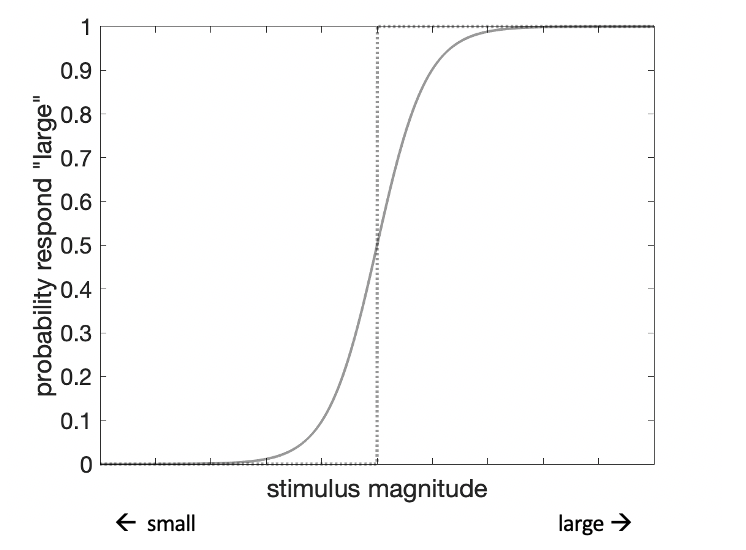
\includegraphics[width=0.7\linewidth]{figures/intro-psychom} 

}

\caption[Psychometric function]{The psychometric function. As an example, an observer may be presented with series of objects of different sizes and asked to categorize each of them as large or small. The x-axis maps the size of each object in the experiment. The y-axis tracks the probability that the observer would categorize a given object as large. The dotted line illustrates a step-wise psychometric function, where all objects above a certain size are always categorized as large and all objects below that size are always categorized as small. By contrast, the solid curve illustrates a typical psychometric function estimated from empirical data.}\label{fig:intro-psychom}
\end{figure}

This characteristic stochasticity of perception posed a puzzle for earlier theories in the field; the advent of signal detection theory \autocite{green1966} ushered in modern thinking about it. Smooth psychometric curves can be explained by the assumption that perceptual choices are based on an internal representation \(\hat{x}\) of the sensory stimulus \(x\) that is corrupted by encoding noise. As suggested by its name, encoding noise arises early on in the processing of a sensory stimulus owing to the intrinsic randomness of neural processes or intrinsic limits on the observability of the stimulus. It is often assumed that encoding noise follows a Gaussian distribution. Consequently, sensory representations may be captured by a random draw from a normal distribution whose mean corresponds to some monotonically increasing function of the magnitude of the true sensory feature and some measure of the variability in the representation:

\begin{equation}
\hat{x} \sim N(f(x),\nu^2) 
\end{equation}

The shape of the transformation \(f(x)\) is classically assumed to follow a logarithmic compression (Weber-Fechner's law for sensory systems), whereby sensitivity to changes in sensory inputs diminishes with the absolute magnitude of stimulation. This phenomenon is ubiquitous across perceptual modalities: the addition of 50g would be easy to notice if we were holding an object weighing 100g; however, we would fail to detect it if the object weighed 1kg. Similarly, we might easily notice the difference between the first and second spoonful of sugar in a cup of tea; noticing the difference between the ninth and tenth would, however, pose a challenge. This characteristic logarithmic compression of sensory magnitudes is an efficient strategy for the neural coding of percepts under the biological capacity constraints of the neural system \autocite{sun2012,wei2017}.

Ideal observer models treat observer choices as inferences about the true stimulus magnitude based on the noisy internal representation (\(\hat{x}\)). An efficient decision rule is a likelihood ratio test against a decision criterion (Neyman-Pearson Lemma). This test compares the ratio of the conditional probability of the observed internal state occurring, given the possible true stimulus magnitudes, against a threshold value.

\hypertarget{optimality-econ}{%
\subsection{Optimality in Economics}\label{optimality-econ}}

In economic analysis, human behavior is explained via the incentives presented by the environment. However, the incentive values of different economic prospects or consumer goods depend on the idiosyncratic preferences of each individual. Thus, compared with psychophysical perception experiments, it is less straightforward to define what the right answer is in any choice situation. Nevertheless, rational choice theory posits that an individual's preferences ought to be transitively ordered and internally consistent.

It is classically assumed that economic decisions elicit decision makers' preferences, which are a fixed function of stimulus characteristics. In the case of uncertain economic prospects (e.g.~gambles with probabilistic outcomes), the expected value is determined by the product of the probability of the event and its magnitude (the monetary outcome). This idea, first introduced by Pascal in the 17th century, provides a benchmark for optimal choice behavior. However, in certain situations, expected value theory leads to choices that appear irrational -- take for instance a lottery ticket offering a 50\% chance of winning £1 million and a 50\% chance of winning nothing. The expected value of this gamble is £500 000 (50\% \(\cdot\) £1 million), and so if someone were to offer to purchase the lottery ticket from us for £499 999, expected value theory dictates we should refuse. Intuitively, however, this choice seems unappealing. In terms of practical changes to our quality of life, the difference between having £499 999 and having nothing (can I afford basic necessities?) is much starker than the difference between having £499 999 and having £1 million (can I afford additional luxuries?).

This idea was formalized by Bernoulli with the example of the St Petersburg paradox \autocite[another hypothetical gamble,][]{dutka1988}, which demonstrates that the \emph{utility} (\(u(x)\), i.e.~subjective value) we attach to economic prospects is a concave function of their expected value \autocite[e.g.~the von Neumann-Morgenstern utility function,][]{vonneumann1944}. Thus, the marginal utility of an additional pound decreases with the total amount of money we have. Expected utility theory has been further refined since to capture the specific rate of decrease of marginal utility as well as risk preferences of individuals \autocite[e.g.~Prospect theory,][]{kahneman1979}. Recent work has demonstrated that the shape of these distortions of expected value constitutes an efficient reward-maximizing strategy under the biological constraints to computational precision in the human brain \autocite{juechems2021}.

These biological constraints are further reflected in the stochastic nature of empirically derived utility functions \autocites[e.g.][]{luce1959,block1960,mcfadden1981}. While traditionally, empirical studies on individuals' choice behavior in economics have used one-off hypothetical scenarios or vignettes \autocite[e.g.][]{kahneman1979}, studies where incentives are varied parametrically have mirrored findings about the stochasticity of choice behavior from perception research \autocite[e.g.][]{mosteller1951}. Therefore, the empirically measured mapping of stimulus features on subjective utility is typically a smooth psychometric curve. The observed smooth, S-shaped psychometric functions can be captured by a stochastic utility representation, where the subjective value function is randomly variable like in sensory perception, \(\hat{u}(x)\) \autocite[as in random utility models,][]{mcfadden1981}. It is usually assumed that, unlike in sensory systems, the source of noise does not stem from early processing stages \autocites[although noise might affect the encoding of both value,][]{bhui2018}[and probability][]{steiner2016}, but rather, from inaccurate retrievals from memory of the true stimulus utility to the individual \autocite[e.g.][]{polania2018}. That is, there is no inaccuracy in the encoding of the identity and characteristics of the option under consideration. Instead, the mapping of the characteristics of the option onto choice is subject to random variability.

\hypertarget{context-dependencies}{%
\section{Context Dependencies}\label{context-dependencies}}

While these normative principles dictate that choices about a target stimulus should be a function of that stimulus alone, human decisions, across perception and economics alike, are often influenced by the context in which they occur.

\hypertarget{perceptual-decisions}{%
\subsection{Perceptual Decisions}\label{perceptual-decisions}}

Human perception is astonishingly context-dependent. A long tradition in perception research has considered that percepts, and the underlying neural responses forming them, are not simply a function of the focal input. Rather, they are a function of the focal input as well as the current background and recent history of stimulation \autocite{webster2015}. The Weber-Fechner law described earlier offers one compelling example of the ubiquity of context dependence. Objectively the exact same stimulus can be more difficult to detect depending on the context in which it occurs. Consider the stars, for instance -- they are practically invisible to us in the daytime under the bright illumination of sunlight, yet at night, in the relative darkness of moonlight, perceiving stars is much easier. Similarly, light pollution in cities, driven for instance by streetlights, makes stargazing a challenge compared to the darker nighttime settings available in the wilderness. Across all those scenarios our perception of the target stimulus (stars) is dramatically affected by the context (illumination provided by sunlight, moonlight or artificial lighting). Below I consider other instances of the influence of temporal or spatial context on our perception.

\hypertarget{temporal-context}{%
\subsubsection{Temporal Context}\label{temporal-context}}

The visual system continuously adapts to the temporal context to ensure that it is maximally sensitive to changes in the inputs that are most likely to occur (i.e.~those close to the mean levels of environmental stimulation). \emph{Adaptation} to contextual levels of stimulation occurs continuously, at multiple time-scales and across multiple domains. Adaptation to light, for instance, can occur at the timescale of seconds and minutes, when moving from outdoors on a sunny day to a dimly lit room, but it also occurs across seasons as the colors dominating our natural environment change \autocite{welbourne2015}, and over the course of the lifetime as the increasing pigment density of the lens in the human eye modifies the spectral composition of light reaching the retina \autocite{webster2015}. The visual system adapts to local low-level stimulus features such as lightness, color and tilt, as well as to more complex, spatially extended characteristics, such as spatial frequency and contrast, and even to composite characteristics, processed at higher levels of the visual hierarchy such as facial attributes and expressions \autocite{webster2011}.

Adaptive effects are canonically repulsive. As the sensory system adapts to the contextual level of stimulation (i.e.~the adaptation level), our experience of incoming stimuli is repelled away from it. Thus, the term repulsion refers to the relationship between our experience of the current stimulus and the properties of context, rather than the interaction between context and stimulus. This independent effect of context means that the same stimulus may be experienced as brighter (or larger) if it were presented following dim (or small) stimuli relative to how it would be experienced when presented following bright (or large) stimuli. Contextual repulsion is typically accompanied by a stimulus-context interaction. The more similar the stimulus to the current adaptation level, the higher the sensitivity of our visual system to changes in the stimulus. That is, small changes in stimulus level close to the contextual expectation are exaggerated.

Computationally, adaptation can be expressed as a shift in the transducer function, linking sensory inputs to neural responses, towards the mean of contextual stimulation (Fig. \ref{fig:intro-adaptation}). The horizontal translation of the transducer illustrates the repulsive influence of context (i.e.~the independent effect of context). This shift, however, also means that the slope of the transducer is steepest around the current environmental expectation, so the neural system is most sensitive to those signals that are most likely to occur (i.e.~the stimulus-context interaction effect). This is an efficient strategy for neurons with limited dynamic range, as it prevents response saturation and maximizes the neural resources dedicated to the processing of the most common signals \autocite{carandini2012}.

Standard place-coding process models of adaptation appealing to this normative principle propose that adaptation impacts the tuning curves of feature-selective populations of neurons (channels), diminishing neural responses to features at (and close to) the adaptation level \autocite[e.g.~for perceptual properties including color contrast, spatial frequency or viewpoint,][]{webster2011}. These diminished responses effectively equate sensitivity across the different channels, such that their average responses are similar within the current context. This outcome can also be achieved through a rate code, where the level of neural responsiveness conveys the stimulus identity \autocite[e.g.~for perceptual properties including saturation, blurriness or facial distortion,][]{webster2011}. Rate-based models of adaptation propose that context neutralizes the intensity of the response, shifting the stimulus level which corresponds to the norm or null point neural response.

\begin{figure}

{\centering 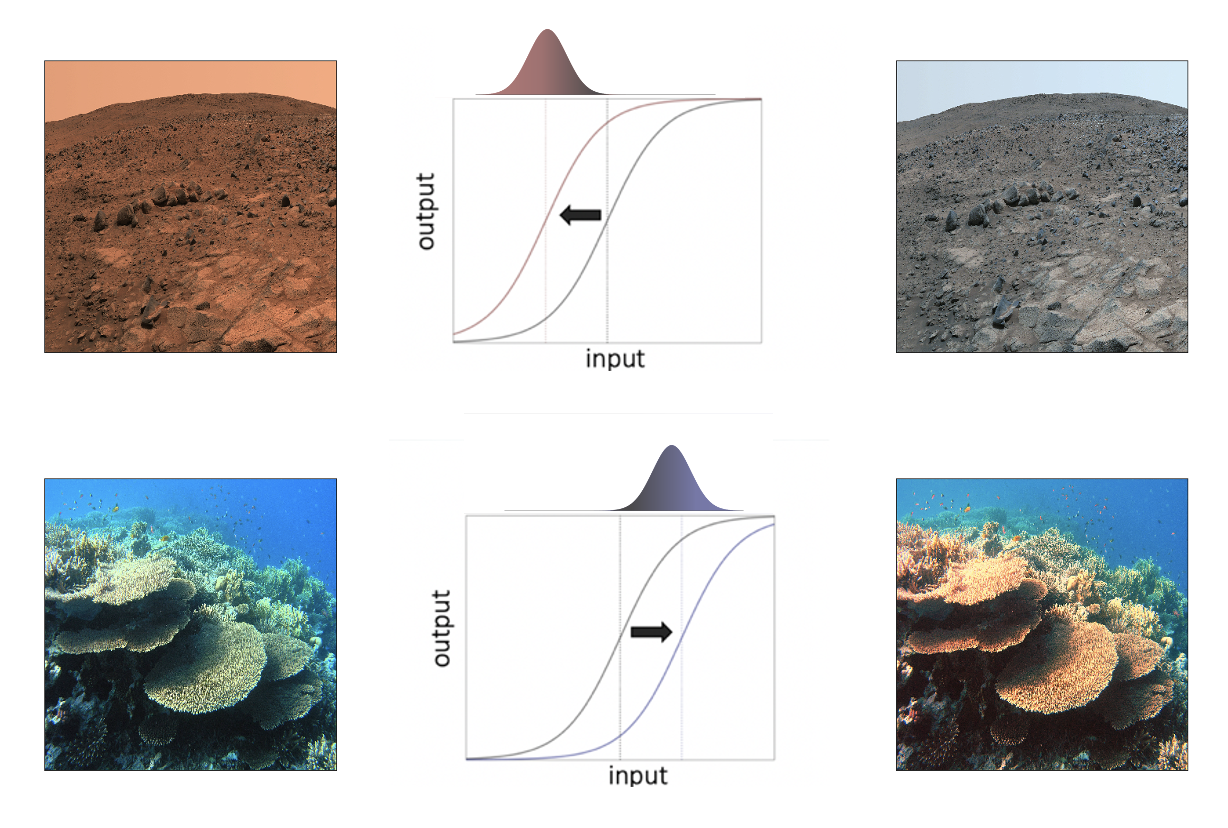
\includegraphics[width=1\linewidth]{figures/intro-adaptation} 

}

\caption[Color adaptation]{Color adaptation. The rightmost column illustrates how the surface of Mars and the sea would appear to a human observer adapted to the landscape of Earth. In the Martian scene, the landscape is dominated by red; in the sea scene -- by blue. The middle column illustrates a neural processing scheme which adaptively shifts the transducer function to track the mean of contextual stimulation (that is, red distribution for Mars; blue distribution for the sea). The leftmost column simulates the appearance of both scenes following adaptation. Both scenes appear more chromatically neutral (adaptive repulsion). Following adaptation to the Martian context, the visual system is fine-tuned to distinguish different shades of red; following adaptation to the sea context -- sensitivity is boosted for change detection in blues. Figure concept adapted from Webster 2015.}\label{fig:intro-adaptation}
\end{figure}

A similar \emph{temporal repulsion effect} is also observed in studies where participants are asked to categorize stimuli according to a perceptual feature (e.g.~as ``big'' or ``small'' according to their size, or as ``heavy'' or ``light'' according to their weight). Regardless of whether participants are given an explicit category boundary (or criterion) against which to compare stimuli \autocites[e.g.][]{lages1998,olkkonen2014} or not \autocites[e.g.][]{helson1947,morgan2000,levari2018}, their choices drift over the course of the experimental session such that the empirical decision boundary effectively tracks the central tendency of the stimulus set. Thus, the same stimulus can be categorized as big or small depending on what other (irrelevant) stimuli the decision maker has recently been exposed to. Beyond the mean, other characteristics of the distribution of stimulus magnitudes, such as its range and skewness, can also sway judgments about sensory stimuli \autocite{parducci1965}. Computational accounts of the repulsive influence of context on categorization judgments have appealed to temporal adaptation \autocite{helson1964,parducci1965}, whereby neural responses to incoming inputs over time are dampened by normalization by the temporal context. An alternative account likens the observed effect to a \emph{contraction bias} in working memory \autocite[also known as central tendency bias,][]{hollingworth1910} affecting the decision maker's reference of the category boundary. This theoretical view proposes that categorization decisions are biased by a drift in the representation of the category boundary towards the prior \autocites[e.g.~midpoint of the stimulus set, contextual expectation, etc.,][]{treisman1984,jou2004,olkkonen2014}. This attractive contextual bias produces a repulsive pattern of behavior, as it affects the categorization criterion against which imperative stimuli are evaluated.

Temporal context effects are not necessarily always repulsive. Indeed, a large literature centers on attractive \emph{serial dependencies} of choice \autocite{kiyonaga2017}. In psychophysical experiments, decisions about a focal stimulus are attracted towards the features of the immediately preceding stimulus, especially if there is a delay between stimulus presentation and response or perceptual ambiguity in the stimulus \autocite{akaishi2014}. This effect is modulated by the degree of similarity between the two sequential stimuli; the more similar the previous stimulus to the current one, the stronger the attraction \autocite{fischer2014}. Normative explanations of this effect appeal to its adaptive role promoting the stability of perception given the statistics of the natural environment \autocite{kiyonaga2017}. The visual world is typically stable over time, so sensory inputs to a given area of the retina are autocorrelated. Thus, in the presence of uncertainty, a Bayesian optimal observer would use previous inputs to resolve the ambiguity \autocite{ashourian2011,olkkonen2014a}. In support of this interpretation, previous work has shown that the stability of environmental statistics can reverse the sign of the sequential dependency effect. For more stable characteristics, such as recognizing the gender of a face, choices are positively associated with the gender of the preceding face, maximizing the stability of perceptions. Conversely, for more changeable characteristics, such as facial expression, choices are negatively associated with the expression of the preceding face, maximizing change detection \autocite{taubert2016}.

\hypertarget{spatial-context}{%
\subsubsection{Spatial Context}\label{spatial-context}}

Some of the most compelling demonstrations of the influence of spatial context come from the domain of color perception, where colors in the spatial vicinity of a focal stimulus can dramatically alter its color appearance. Fig. \ref{fig:intro-constancy} illustrates how the same physical color (i.e.~spectrum of wavelengths emanated from a given region) can be perceived differently depending on what colors surround it. This dependence on spatial context has an adaptive purpose -- it gives rise to \emph{color constancy} or our ability to experience the color of an object (i.e.~the perceptual correlate of spectral reflectance) as unchanging despite changes in the spectral composition of the illuminant. Thus, processing color signals in a relative manner, rather than in isolation, allows the neural system to solve the otherwise mathematically intractable task of interpreting the light signals reaching the retina in a way that separates an object's surface color from the color of lighting \autocite{smithson2005}. While the specific computational mechanisms underlying this phenomenon are still the topic of debate, a popular theme across proposals suggests that cone cell excitation signals in the retina are normalized by a quantity set by the context \autocite{land1983,foster2011}.

\begin{figure}

{\centering 
\includegraphics[width=1\linewidth]{figures/intro-constancy} 

}

\caption[Color constancy]{Color constancy. On the painting on the left, the circled region on the demarcated flower petal appears red, but is actually gray. On the painting on the right, the circled region on the demarcated flower petal appears blue, but is also gray. Painting by Rachel Ruysch, ca. 1680.}\label{fig:intro-constancy}
\end{figure}

Spatial dependencies in visual processing have been documented across a variety of other domains, including the perception of orientation and contrast. A classic example is the \emph{tilt illusion} \autocite{blakemore1970} where the tilt of a central grating is repulsed from the tilt of flanking gratings. Thus, a central horizontally oriented stimulus would appear tilted clockwise, when surrounded by anticlockwise flankers. Similarly, spatial context repels contrast perception. A central texture appears of lower contrast when surrounded by a high contrast texture compared to when surrounded by a uniform background \autocite{chubb1989,xing2001}. The repulsive influences of context across visual attributes have been successfully modeled in a normalization framework, whereby neural responses to target inputs are normalized by the features of context \autocite{carandini2012}.

Another example of spatial dependencies in perception comes from the literature on \emph{lateral interactions} \autocite{stemmler1995}. Psychophysical and electrophysiological evidence converges on a pattern of \emph{contextual facilitation} in visual processing whereby the presence of proximal stimuli lowers thresholds for the detection of \autocite{kapadia1995,freeman2001,freeman2005} and boosts neural responses to \autocite{kapadia1995,ito1999} a collinear target stimulus. Crucially, this contextual effect can reverse its direction. When target stimuli are close to detection thresholds, flanking stimuli often facilitate processing \autocite{polat1993}. For high-contrast targets, on the other hand, lateral interactions are, generally, of a suppressive nature \autocite{stemmler1995}. These characteristics of lateral interactions have been linked with the behavioral relevance of visual context in the real world. Context can be helpful to identify and interpret stimuli near detection thresholds \autocite{gilbert2000}. For example, neighboring visual inputs may be useful when the visual system is trying to make sense of blurry or interrupted lines on a faded photograph. Ambiguity is, however, lower for suprathreshold stimuli, so the visual system need not rely on contextual clues for stimulus identification. Instead, \emph{contextual inhibition} may aid the quick detection of changes in the visual environment through pop out effects for inconsistent stimuli \autocite{stemmler1995}.

\hypertarget{economic-decisions}{%
\subsection{Economic Decisions}\label{economic-decisions}}

Over the past 40 years, the field of behavioral economics has cataloged instances of ``suboptimal'' context-dependent economic behavior \autocite{thaler2015}. From the standpoint of classical economics, these phenomena constituted ``anomalies'' from rational behavior. Despite the many commonalities between context dependence in perception and economics, the interpretations of the observed patterns of contextual influence have been starkly different between disciplines. In perception research, context dependencies have generally been interpreted in an adaptive light, allowing the perceptual system to take advantage of regularities in the environment to enhance efficiency in sensory processing (e.g.~normalization-based neural coding) and resolve perceptual ambiguity (e.g.~Bayesian inference). In economics, they have predominantly been considered as instances of irrationality \autocite{kahneman1991} and normative explanations of context-dependent choice behavior have largely been overlooked till fairly recently \autocite{loewenstein2008}.

\hypertarget{temporal-context-1}{%
\subsubsection{Temporal Context}\label{temporal-context-1}}

Economic choices regarding monetary rewards are characterized by repulsion effects akin to the temporal context biases documented in perceptual categorization discussed above. When the reward context (as defined by the mean of rewards experienced in previous trials) changes, so too does a participant's subjective valuation of rewards (as estimated by their choice behavior) shift. In a high-reward context (e.g.~average reward = £5), participants generally value the same monetary sum (e.g.~£5) less than they do in a low-reward context \autocite[e.g.~when average reward = £3,][]{rigoli2016}. In line with the observed \emph{context-dependent valuation} behavior of humans, electrophysiological evidence from non-human primates \autocite{tremblay1999,padoa-schioppa2009} and fMRI evidence from humans \autocite{cox2014} in tasks where the reward context is manipulated suggests that value is not encoded in an absolute fashion. Rather, neural value signals are consistent with an encoding scheme whereby stimulus value is processed relative to the recent reward history \autocite{rangel2012}. Context-dependent subjective value decisions are affected by the mean \autocite{rigoli2016}, variability \autocite{rigoli2016}, and skewness \autocite{stewart2006} of the distribution of previously experienced rewards in a direct parallel with context-dependent perceptual categorization \autocite{parducci1965}. Accordingly, popular computational accounts of this effect appeal to normalization, whereby target values are divisively normalized by a summary characteristic of the distribution of contextual levels of stimulation, such as the average \autocite[as in divisive normalization,][]{louie2013}, average and variability \autocite[as in the logistic model of subjective value,][]{rigoli2019}, or range \autocite[as in range normalization,][]{padoa-schioppa2009}. A more extreme theory of relative value, decision by sampling, argues that the subjective value of a stimulus is entirely driven by the stimulus' ranked order within the context \autocite{stewart2006,heng2020}.

Outside of the lab, this temporal repulsion effect has been observed in the prices of properties rented by individuals who have recently moved to a new city. In line with reference-dependent valuation, those arriving from relatively cheaper cities rent cheaper properties compared to those arriving from more expensive cities, regardless of movers' objective wealth \autocite{simonsohn2006}. In the marketing literature, a related concept is the so called \emph{perceptual contrast} \autocite{lynchjr.1991,tormala2007,lee2010}, where a consumer's evaluation of a target good is repulsed away from their evaluation of a decoy good with which they were presented immediately before this. For instance, a retail agent might first show a prospective client a very unattractive property in order to boost the subjective value of a subsequent target property for the client \autocite{cialdini1987}. Naive home buyers are far from the only victims of this bias. Experienced financial professionals are also swayed by contrast effects, such that investors' evaluations of today's earnings are inversely proportional to their balance from the previous day \autocite{hartzmark2018}.

Conversely, \emph{anchoring} refers to the systematic assimilation of subjective evaluations of a target stimulus to an immediately preceding, unrelated and arbitrary reference magnitude \autocite{tversky1974}. The induction of an anchoring effect typically requires a comparison between the target evaluation and the anchor. For instance, Ariely and colleagues \autocite*{ariely2003} first asked a cohort of MBA students if they would be willing to purchase a variety of consumer goods, such as wine bottles, computer accessories or books, for a price equal to the last two digits of their social security number (the anchor). Then, the researchers asked participants to report the maximum price they would be willing to pay for each good. Value estimates were strongly influenced by the arbitrary anchor; higher anchors inflated the reported price, while lower anchors diminished it. Anchoring has been observed across a variety of domains, including economic valuation, general knowledge and factual estimates, probability estimates, legal judgments, and negotiations \autocite{furnham2011}.

\hypertarget{spatial-context-1}{%
\subsubsection{Spatial Context}\label{spatial-context-1}}

A classic example of the influence of spatial context in economics is the \emph{decoy effect}. It refers to the finding that consumer choices between two equally preferred options, which vary along two dimensions, can be swayed by the addition of a third, generally inferior, alternative. The introduction of a dispreferred, and hence termed decoy, option should not in theory affect the choice between two better alternatives \autocite{block1960}. However, value judgments are systematically affected by decoys. First described in 1982 \autocite{huber1982}, the \emph{asymmetric dominance} (or attraction) effect is produced by a decoy good which is dominated asymmetrically, that is, it is objectively worse than one of the two target options, but not the other. Consumer choice is attracted towards the dominating alternative. For instance, when choosing between a cheap but slow computer and a pricey but fast one, the addition of an alternative which is slightly more expensive than the cheap one yet just as slow boosts preference for the cheap computer.

In a similar vein, a decoy which is similar to one of the two alternatives repels choice away from it \autocite[\emph{similarity effect}][]{tversky1972} and a decoy which is more extreme than one of the options, but equally preferred, sways choice towards it \autocite[\emph{compromise effect},][]{simonson1989}. All three classic decoy effects have been replicated in the domain of perceptual decisions, using judgments about the area of rectangle stimuli of varying height and width \autocite{trueblood2013}. This finding suggests that the decoy effect is likely driven by a general principle in decision processing across stimulus domains. In line with this explanation, the most recent computational accounts of the decoy effect have proposed normalization in the neural coding of decision inputs as the driver of the observed context dependencies \autocites[e.g.][]{rigoli2017,bushong2021,daviet2021,landry2021}.

Another finding in multialternative choice concerns \emph{value distraction} \autocite{louie2013}. It occurs when choosing between two items, one of which is preferred by the decision-maker, such that \(v(A)>v(B)\). The value of a third option, inferior to the two original alternatives (\(v(D)<v(B)<v(A)\)), affects how often the option with the subjectively highest value is chosen. The probability that both humans and non-human primates would select option A over B falls as the value of the distractor option grows \autocite[in speeded choices as in][]{louie2013} and reaction times rise \autocite[in slower settings in humans as in][]{gluth2020}. This context dependence can be explained in a normalization framework, where choice values are divisively normalized by the (weighted) sum of context. As the distractor value rises, so does the numerator in the normalization procedure, lowering sensitivity to value differences between A and B \autocite{louie2013}. An alternative account, drawing on a sequential sampling tradition, proposes that high value distractors capture the decision maker's attention and thus bias behavior \autocite{gluth2020}.

\hypertarget{parallels}{%
\subsection{Parallels}\label{parallels}}

Perceptual and economic decisions have largely been the focus of two distinct research streams and this separation is reflected in divergences in methodology. Perception research often employs weak or noisy stimuli, striving to measure (changes to) an observer's threshold for stimulus detection or discrimination. Perceptual decision making studies typically involve a long, repetitive sequence of choice trials. The large amount of data from each participant allows researchers to parametrically investigate how different levels of an input of interest affect the choices of the observer. By contrast, economic decisions have traditionally been studied via one-shot hypothetical scenarios or vignettes, where each participant provides one (or very few) data points; although recently, psychophysical investigations have become more common in economics.

Beyond these differences in methodology, by definition, economic and perceptual judgments concern qualitatively vastly different inputs and operations. Perceptual decisions target some existing property of the world, such as the appearance of an object; by contrast, economic decisions deal with the decision maker's preferences, such as their subjective valuation of the object. The sources of uncertainty are therefore different. In perceptual choice, it is largely the inputs that are uncertain (what is there?); in economic choice, it's the value function (how much do I value it?).

Nevertheless, there are also commonalities. Across both domains, the goal of the decision maker is, generally, to compare the available options and select a course of action. The rich, high-dimensional and noisy evidence for each alternative must be integrated and translated into a discrete low-dimensional outcome -- the decision \autocite{summerfield2020}. Indeed, a growing literature attempts to draw bridges between perceptual and economic decisions \autocite{summerfield2012,woodford2020} highlighting commonalities in their behavioral signatures, neural underpinnings and computational models thereof. Another set of parallels between perceptual and economic choices emerges in the ways in which they can be affected by context.

First, the law of diminishing marginal utility strikingly mirrors the Weber-Fechner law of perception. As the absolute magnitude grows, small changes in magnitude become increasingly difficult to notice. These logarithmic compressions, across both perception and valuation, have been linked with the limited capacity of the neural system \autocites[e.g.][]{wei2017,bhui2018}. Calibrating sensitivity to the relevant range of magnitudes in the context makes the most efficient use of the limited dynamic range of neural firing. This parallel suggests that there might be a common principle principle guiding the processing of decision-relevant information across the two domains \autocites{woodford2020}[although interestingly, Max Weber himself was skeptical of this idea,][]{weber1975}. It also gives rise to symmetric contextual biases in the evaluation of magnitudes, effectively scaling percepts and subjective valuations of changes in an imperative stimulus according to its absolute magnitude.

Judgments across perception and economics also exhibit analogous and robust reference dependence. Information in the temporal context of a decision sets the reference against which incoming inputs are judged. In a context dominated by large (or valuable) objects, a focal stimulus may be perceived (or evaluated) as small (or unappealing). That same stimulus can be judged as large (or valuable) in a context of small (or unappealing) objects. Quantitatively, this pattern of results is captured by a drifting psychometric function which tracks the contextual expectation. Across both domains, other features of the statistics of context affect judgments, including the shape, skewness and dispersion of the distribution of feature magnitudes present \autocite{parducci1965,rigoli2019}. Reference-dependent percepts and valuations have commonly been modeled as the result of an adaptive process, whereby neural signals are normalized by the contextual levels of stimulation \autocite{webster2015,rigoli2016}. In line with this theoretical view, across the processing hierarchy neural responses to visual stimuli and economic prospects exhibit contextual adaptation \autocites[e.g.][]{enroth-cugell1973,cox2014}.

Reference-dependent judgments are typically repelled \emph{away} from context. However, another class of contextual biases sways choices across perception and economics \emph{towards} context. In the domain of perception, judgments about a focal stimulus can be attracted towards the stimulus immediately preceding it if the two stimuli are sufficiently similar and located nearby to one another \autocite{liberman2014,st.john-saaltink2016,barbosa2020}. In the domain of economics, a value estimate of a prospect can be attracted towards a preceding irrelevant quantity if a direct comparison has been drawn between the two. This can be done, for instance, by asking if the subjective value of the prospect exceeds the anchor quantity \autocite{tversky1974}. Sequential dependencies across both perceptual and economic judgments can be strengthened in the presence of noise, including increased stimulus-response intervals and scalar variability \autocite{papadimitriou2016,lee2021}.

The influence of spatial context also encompasses repulsive and attractive effects, whose strength and directionality typically interact with the imperative stimulus. For instance, the decoy effect has been documented in multialternative choices about economic prospects and visual stimuli alike \autocite{trueblood2013}. The decoy stimulus can sway choices towards different alternatives depending on the interplay of attribute values of all available options. Similarly, the effect of spatial context on perceptual detection judgments can reverse its direction depending on the characteristics of the focal stimulus \autocite{stemmler1995}. This pattern of results suggests that inputs are processed differently depending on their interrelationship with other information present in the spatial context. This idea has also been formalized in normalization frameworks where neural responses are modulated by context \autocite{xing2001,daviet2021}.

The influence of context on human information processing and decision making extends beyond the realms of perception and economics. As early as the 1960s, research documented the dynamics of contextual repulsion and attraction in human affect, motivation, learning, cognition and interpersonal behavior \autocite{helson1964}. A popular account in perception, adaptation-level theory posits that the human brain processes information across all manner of input domains, including low-level sensory stimulus features and more high-level abstract concepts and characteristics, in a relative, context-dependent manner. The existing parallels in context dependencies across perceptual and economic decision domains lend support to the view that there might be a domain-general information processing mechanism which gives rise to contextual influence.

\hypertarget{the-underpinnings-of-context-dependent-choice}{%
\section{The Underpinnings of Context-Dependent Choice}\label{the-underpinnings-of-context-dependent-choice}}

What drives context dependencies in choice? In biology, there is an important distinction between proximate and ultimate explanations. Proximate causes capture the mechanisms directly driving a behavior (e.g.~observed patterns of neural activity or inferred information processing mechanisms); ultimate causes refer to the evolutionary origins that have selected for and shaped the behavior \autocite{davies2012}. Normative perspectives of decision making serve as clues for the selective pressures shaping choice behavior. For this, I will turn back to normative views of decision making to explore the ultimate causes underlying context-dependent choice. This section redefines what constitutes an optimal decision by incorporating assumptions about constraints to the decision making process, including the limited capacity of the brain \autocite{sims2003} and the inherent noisiness of neural computation \autocite{tsetsos2016}.

\hypertarget{neural-constraints-efficiency}{%
\subsection{Neural Constraints \& Efficiency}\label{neural-constraints-efficiency}}

The discussion in section \ref{optimality} regarding what constitutes an optimal decision assumed that neural systems are, generally, free from processing constraints. While acknowledging that neural representations are noisy, the models described in sections \ref{optimality-perc} and \ref{optimality-econ} neglect the limited capacity of the human nervous system and the metabolic costs associated with information processing. In cognitive science, these constraints would be reflected in the cost function of the processing system, which is minimized in efficient calculations. These efficiency considerations are reflected in the \emph{efficient coding} hypothesis \autocite{barlow1961,simoncelli2003}.

An efficient strategy for the encoding of sensory information postulates that neural representations should follow the environmental statistics \autocite{girshick2011}, resulting in the observed overrepresentation of, for instance, cardinal orientations in early visual cortex \autocite{furmanski2000,li2003}. This strategy, whereby the distribution of possible neural states matches the structure of the environment, ensures that sensitivity is maximized for the features which are most likely to occur.

While the concept of efficient coding is generally associated with evolutionary and developmental neural adaptations to the natural environment \autocite{barlow1961}, similar processes are operating at much shorter time-scales, adapting the neural system to the levels of stimulation available in the local context. Light adaptation offers an example of this -- adaptation to the contextual level of light dedicates the limited neuronal range (typically \textasciitilde2 orders of magnitude) to those light intensities which are present in one's immediate environment, and ensures that visual sensitivity is relatively stable despite changes in light levels of a factor of over 10 billion \autocite[or \textasciitilde10 orders of magnitude,][]{stockman2006}. Adaptation, thus, is an efficient strategy given the biological constraints of the visual system; it does, however, also lead to context dependence in our percepts \autocite{webster2015}. Theoretic approaches from economics, such as bounded rationality \autocite{simon1955} and rational inattention \autocite{sims2003}, have similarly appealed to the constraints of human information processing to explain the mechanisms driving context-dependent economic choice.

Normalization has been put forth as a ``canonical operation'' adapting the neural system to current levels of stimulation and promoting the efficiency of neural computation across the processing hierarchy \autocite{carandini2012}. Generally, normalization theories involve the multiplicative normalization of neural signals by a common factor drawn from, for instance, the activity of a neuronal population. The specific mathematical formulation of the normalization factor is the topic of debate \autocites[e.g.~the weighted sum of inputs as in][]{carandini2012,louie2013}[or the range of inputs as in][]{soltani2012}. However, a commonality across specific accounts is that normalization concentrates the available range of neural responses around some estimate of what inputs are most likely to occur. This, in turn, ensures that various efficiency considerations are met, including maximizing sensitivity to changes in inputs, boosting sensitivity for behaviorally relevant stimuli, avoiding neural saturation and reducing neural redundancy. Divisive normalization occurs across many different stimulus domains and computational operations, including sensory processing, attention modulation, the encoding of value and multisensory inference \autocite{carandini2012}.

Implementation-wise, normalization has been documented across various scales of neural processing. For instance, on the single neuron level, neural responses to a constant stimulus are adapted via inhibiting intrinsic ionic currents based on the neuron's own activity \autocite[inhibitory feedback loop,][]{benda2021}. Normalization-based inhibition can also occur via lateral cortical connections, whereby stimuli outside the classic receptive field of a neuron can adjust that neuron's response to stimulation within its receptive field center \autocite{stemmler1995}. Similar dynamics have also been observed on the population level, for instance, pooled inhibition in the posterior parietal cortex, which may play a role in decision making pertaining to categorical choices \autocite{wang2002}.

\hypertarget{behavioral-relevance}{%
\subsection{Behavioral Relevance}\label{behavioral-relevance}}

Beyond the case for computational efficiency, relative decision making may also confer some behavioral advantages. The idea that evaluating stimuli relative to the local context is an efficient and evolutionary adaptive strategy is a central tenet of \emph{optimal foraging theory} \autocite{stephens1986,kolling2012}. An animal should choose whether to exploit a given resource or explore for other resources, depending on an estimate of the current resource value relative to the expected environmental reward. Relative perception and valuation can similarly be argued to serve an adaptive behavioral function.

Context can also help resolve ambiguities. A popular normative principle for decision making which incorporates the contextual expectation is \emph{Bayesian decision theory} \autocite{mamassian2002,yuille2006}. According to this theoretic account, an ideal observer should evaluate a stimulus taking into account not only the likelihood of the true stimulus magnitude given the noisy internal representation (\(\hat{x}\)), but also the prior expectations about the likelihood of this magnitude occurring. These prior expectations are shaped by context and follow the distribution of signals that are currently present or recently experienced. Thus, signal inferences for the true magnitude of \({x}\) will be biased towards the contextual expectation. A similar theoretical framework underpins dominating accounts of the contraction bias, appealing to Bayesian inference to explain the finding that the influence of the prior grows with the presence of noise in the judgment process \autocite{ashourian2011,olkkonen2014}.

In signal detection theory, prior expectations may be incorporated in the parameter value of the decision criterion, which sets a threshold that needs to be exceeded for a detection judgment to occur \autocite{green1966}. While this can make detection judgments more liberal in a context where the signals of interest dominate, the criterion is classically considered stable over time. \emph{Criterion setting theory} \autocite{treisman1984,lages2010} is an extension of signal detection theory which instead argues that the location of the decision criterion drifts over time according to two opposite mechanisms which both work to further the behavioral goals of the observer. The probability tracking mechanism is driven by the autocorrelated nature of inputs in the natural environment: if a signal was present at \(t-1\), then it is more likely to be present than not at time \(t\). Hence, it leads to cross-trial attractive serial dependencies. The stabilization mechanism, on the other hand, shifts the criterion towards the central tendency of context in order to ensure that positive and negative detection judgments occur equally often, maximizing information transmission. This, in turn, leads to reference-dependent judgments that are repelled from the statistics of local context.

The attractive and repulsive dynamics of contextual influence can, thus, be traced back to the interplay of efficiency considerations and the behavioral relevance of context. In the real world, our visual (and conceptual) environment is stable. The neural system explores this regularity to promote efficient computation and increase sensitivity to small changes in the environment \autocite{mattar2018}. This efficient adaptation of neural coding produces \emph{repulsive} influences of context \autocite{webster2015,fritsche2020}. The spatially and temporally correlated nature of inputs, however, also gives rise to \emph{attractive} contextual effects. A Bayesian observer would exploit the stability of the environment when decoding noisy sensory inputs, with contextual information guiding the prior probability of target signals. Thus, judgments would be attracted towards the statistics of context \autocite{vanbergen2019,fritsche2020}. Taken together, these two opposite efficient strategies can explain the rich (and contradictory) patterns of contextual influence outlined here: negative context dependence is optimal in encoding information, but positive context dependence is optimal when decoding neural signals \autocite{fritsche2020}.

\hypertarget{thesis-outline}{%
\section{Thesis Outline}\label{thesis-outline}}

Human choices often exhibit stereotyped patterns of context dependence. This is true across decisions pertaining to the evaluation of low-level sensory features, such as visual or auditory properties, and high-level features, such as subjective value, propositional statements and abstract concepts. The parallels between context-dependent choices in perception and economics reviewed in this chapter suggest that there might be a common, domain-general decision mechanism underlying these phenomena \autocite{helson1964}. The neural underpinning of such a mechanism could stem from neural efficiency considerations. State-of-the-art psychophysical, electrophysiological and neuroimaging evidence suggests that normalization is a feasible candidate domain-general computational scheme.

This thesis explores specific instances of context-dependent choice behavior. Chapter 2 charts the full parametric space of decoy influence in economic decisions and arbitrates between different formalizations of neural normalization. Chapter 3 investigates and models the functional form of the effect of a distractor stimulus in a perceptual discrimination task. Chapter 4 arbitrates between opposing theoretical accounts of reference-dependent perceptual categorization.

\begin{savequote}
\emph{This chapter is based on the published work:}

Dumbalska, T., Li, V., Tsetsos, K., \& Summerfield, C. (2020). A map of
decoy influence in human multialternative choice. Proceedings of the
National Academy of Sciences, 117(40), 25169-25178.
\qauthor{}\end{savequote}

\hypertarget{decoy}{%
\chapter{A map of decoy influence in multialternative economic choice}\label{decoy}}

\minitoc

\noindent 
\emph{When choosing between two alternatives, the addition of a third inferior option should not affect choices. In practice, however, even though the dispreferred decoy good is rarely chosen, it can systematically sway preference towards one of the two original alternatives. Previous work has identified three classic decoy biases, known as the attraction, similarity and compromise effects, which arise during choices between economic alternatives defined by two attributes. However, the reliability, interrelationship, and computational origin of these three biases has been controversial. Here, a large cohort of human participants made incentive-compatible choices among assets that varied in price and quality. Instead of focusing on the three classic effects, we sampled decoy stimuli exhaustively across bidimensional multiattribute space and constructed a full map of decoy influence on choices between two otherwise preferred target items. Our analysis revealed that the decoy influence map was highly structured even beyond the three classic biases. We identified a very simple model that can fully reproduce the decoy influence map and capture its variability in individual participants. This model reveals that the three decoy effects are not distinct phenomena but are all special cases of a more general principle, by which attribute values are repulsed away from the context provided by rival options. The model helps understand why the biases are typically correlated across participants and allows us to validate a new prediction about their interrelationship. This work helps clarify the origin of three of the most widely studied biases in human decision-making.}

\hypertarget{introduction-1}{%
\section{Introduction}\label{introduction-1}}

Optimal decisions should be driven solely by information that is relevant for the choice. When deliberating among more than two options (``multialternative'' choices) this means ignoring those alternatives that are inferior or unavailable. Hence, the choice between two consumer goods should not be affected when an unaffordable third option is introduced. Similarly, voting preferences between two electoral candidates should not be changed when a third contender with more dubious merit enters the race. This normative principle, which is enshrined in the axiom of regularity \autocite{block1960,rieskamp2006}, has been of significant and long-standing interest to behavioral scientists as it is robustly violated by a variety of animals including humans \autocite{tversky1972a,huber1982,simonson1989}, monkeys \autocite{parrish2015}, amphibians \autocite{lea2015}, invertebrates \autocite{shafir1994}, and even unicellular organisms \autocite{latty2011}. The existing empirical evidence has indicated that where choice alternatives are characterized by two value dimensions (e.g.~the price and the quality of a product or the likability and competence of a political candidate), the introduction of an irrelevant distractor item to the choice set leads to rich and stereotyped biases in decision-making. A key research goal in the fields of psychology and economics has been to identify a simple and elegant computational principle that can explain the biases provoked by an irrelevant ``decoy'' stimulus \autocite{turner2018}.

The existing literature has focused on three decoy effects that can arise during ternary (three-way) choice among alternatives characterized by two independent and equally weighed attributes. The phenomena are illustrated in Fig. \ref{fig:decoy-illustr}. Consider for example a consumer who is choosing between three products that are each characterized by dimensions (attributes) of quality and economy. The axes in Fig. \ref{fig:decoy-illustr} are scaled such that these attributes are perfect substitutions in that the consumer will forego one unit of one attribute for one unit of the other. Two target items, A and B, lie on the line of isopreference which is perpendicular to the identity line. In other words, A is less expensive but lower quality than B, such that the consumer should be indifferent between these options. The empirical phenomena describe how preferences may be biased towards either A or B as a function of a third ``decoy'' item D that lies on or below the isopreference line. The consensus view holds that a bias towards A can be provoked by the inclusion of a decoy \(D_a\) that it dominates, that is where A (but not B) is equivalent or superior on both dimensions (the attraction effect); that a bias towards A occurs in the presence of a more extreme decoy \(D_c\) which is superior in quality but yet more expensive than A, making A the ``compromise'' option (the compromise effect); and that a bias towards A is incurred by a decoy \(D_s\) which is similar to B in price and quality (the similarity effect, Fig. \ref{fig:decoy-illustr}).

\begin{figure}

{\centering 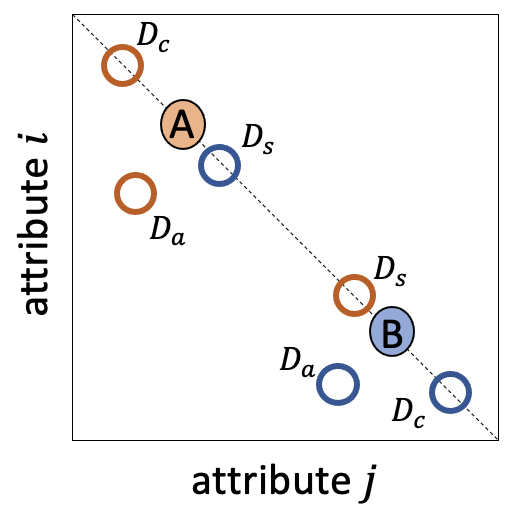
\includegraphics[width=0.5\linewidth]{figures/decoy-illustr} 

}

\caption[Decoy effects]{Illustration of the attraction, compromise and similarity effects. A and B denote two equally preferred stimuli; A is strong on attribute $i$ but weak on attribute $j$ and vice versa. The introduction of decoy stimuli (rings; denoted $D_a$, $D_c$ and $D_s$) can bias preferences towards either A or B. The color of each ring signals the direction of the bias, e.g. for orange rings, A is preferred. Stimuli falling on the dashed line are equally preferred.}\label{fig:decoy-illustr}
\end{figure}

These three phenomena have been a major object of study in psychology and behavioral economics for several decades, with research interest reinvigorated in the last couple of decades after a landmark study that proposed the first unified computational account of the three classic decoy effects \autocite{roe2001}. Since then, a variety of empirical results have been produced and a plethora of computational models have emerged. These include models that rely on loss aversion \autocite{tsetsos2010}, pairwise normalization \autocite{landry2021}, attentional weighing \autocite{hotaling2010,tsetsos2012,bhatia2013,trueblood2014}, lateral inhibition \autocite{hotaling2010}, associative biases \autocite{bhatia2013}, power-law transformation of attribute values \autocite{bhatia2013}, sampling from memory \autocite{noguchi2014,bhui2018}, or various other forms of reference-dependent computation \autocite{soltani2012,li2018,natenzon2019,rigoli2019}. However, there has been a notable lack of consensus about the computational principles that give rise to decoy effects \autocite{turner2018}. There are a number of potential reasons for this, but here we focus on one limitation of past studies: most have tested for decoy effects by selecting fixed attribute values for \(D_a\), \(D_c\) and \(D_s\) and calculating for each the relative choice share (RCS) for target items A and B, with relative deviations from choice equilibrium signalling a bias indicative of the successful detection of a decoy effect. However, reducing the dimensionality of the data in this way (i.e.~to 6 data points) makes it harder to distinguish theoretical accounts, as many models may mimic one another in successfully capturing the phenomena, so that comparisons among models are reduced to questions of a priori plausibility and parsimony. Relatedly, what defines a ``decoy'' of each class is typically left largely to the discretion of the researcher, who is free to choose a priori the values for \(D_a\), \(D_c\) and \(D_s\) -- i.e.~the space over which the attraction, compromise or similarity might occur. This issue, coupled with the fact that the effects are often studied in small participant cohorts, using diverse stimulus materials -- consumer choices \autocite{josiam1995}, text-based vignettes \autocite{yang2014}, or perceptual judgments \autocite{trueblood2013} -- has led to disagreement over the provenance and reliability of the three effects \autocite{trueblood2012,frederick2014,yang2014,trueblood2015}.

In this chapter, we address these issues by reporting a large-scale (\(n>200\)), incentive-compatible study. We systematically mapped the decoy influence across attribute space, calculating the relative choice share \(RCS_{ij}\) for each decoy with attribute values \(i\) and \(j\). This allowed us to explore the dimensionality of the data, with a view to asking whether a single principle can explain the ensemble of observed decoy effects. We found that a remarkably simple model, which draws on a computational framework based on the principle of divisive normalization, can capture the full decoy influence (RCS) map. Importantly, the model suggests that the three canonical decoy effects are not in fact distinct phenomena but rather fall naturally out of previously described dynamics of attraction and repulsion of decision values towards and away from a reference value given by the mean of available options.

\hypertarget{experiment}{%
\section{Experiment}\label{experiment}}

\hypertarget{methods}{%
\subsection{Methods}\label{methods}}

\hypertarget{participants}{%
\subsubsection{Participants}\label{participants}}

A total of 358 US-based participants were recruited via the platform Amazon Mechanical Turk to participate in a three-phase online study. All participants took part in the first phase (rating task), and those who passed a performance threshold (\(n=231\); see below) were invited to join the second and third parts of the study in separate testing sessions (choice task). Of these, 189 met our criteria for inclusion in the analysis, namely \(p<0.001\) of responding randomly during the choice task (binomial test). Phases 2 and 3 (choice task) were identical; phase 3 simply allowed us to gather more data (\(n=149\) completed both phases 2 and 3). Data were collected in two distinct batches. In the first batch, we paid participants \$4 for completing each phase, in addition to a performance-based bonus of up to \$20 for the second and third part of the study (a maximum payment of \$32). To reduce the dropout rate, in the second batch the base payment was increased to \$5 and the bonuses increased to \$12 and \$18 in the second and third phases respectively (a maximum payment of \$45). The study received ethical approval from the Central University Research Ethics Committee at the University of Oxford (approval reference number: R50750/RE001).

\hypertarget{experimental-tasks}{%
\subsubsection{Experimental Tasks}\label{experimental-tasks}}

\hypertarget{rating-task}{%
\paragraph{Rating Task}\label{rating-task}}

The first phase of the study (rating task, Fig. \ref{fig:decoy-methods}a) was introduced as a ``property rental price guessing game''. The task involved estimating the market rental price of residential real estate by viewing an image of the exterior of a series of properties. On each trial, an image of a property was shown along with a horizontal slider for a maximum of 60 seconds. The task was to guess the market rental price of the property, i.e.~the dollar amount that an average person would be willing to pay per month to rent it, and to indicate it on a slider scale. The slider ranged from \$0 to \$2500 and the initial position of the slider was randomized on each trial. There were a total of 250 unique house images, each presented twice in randomized order (for a total of 500 trials per participant). The 250 houses had been selected to have the lowest average choice variability in a pilot study involving 30 distinct participants and a larger set of properties (\(n=450\)), which we conducted before the main experiment. We used participant ratings from the pilot dataset to include/exclude participants. After phase 1, we correlated the 250 ratings for each participant against the average ratings obtained from the pilot study. Participants with a Spearman's rank correlation of \(\rho< 0.7\) were excluded; the rest (\(n\) = 231) were invited to progress to the choice task.

\begin{figure}

{\centering 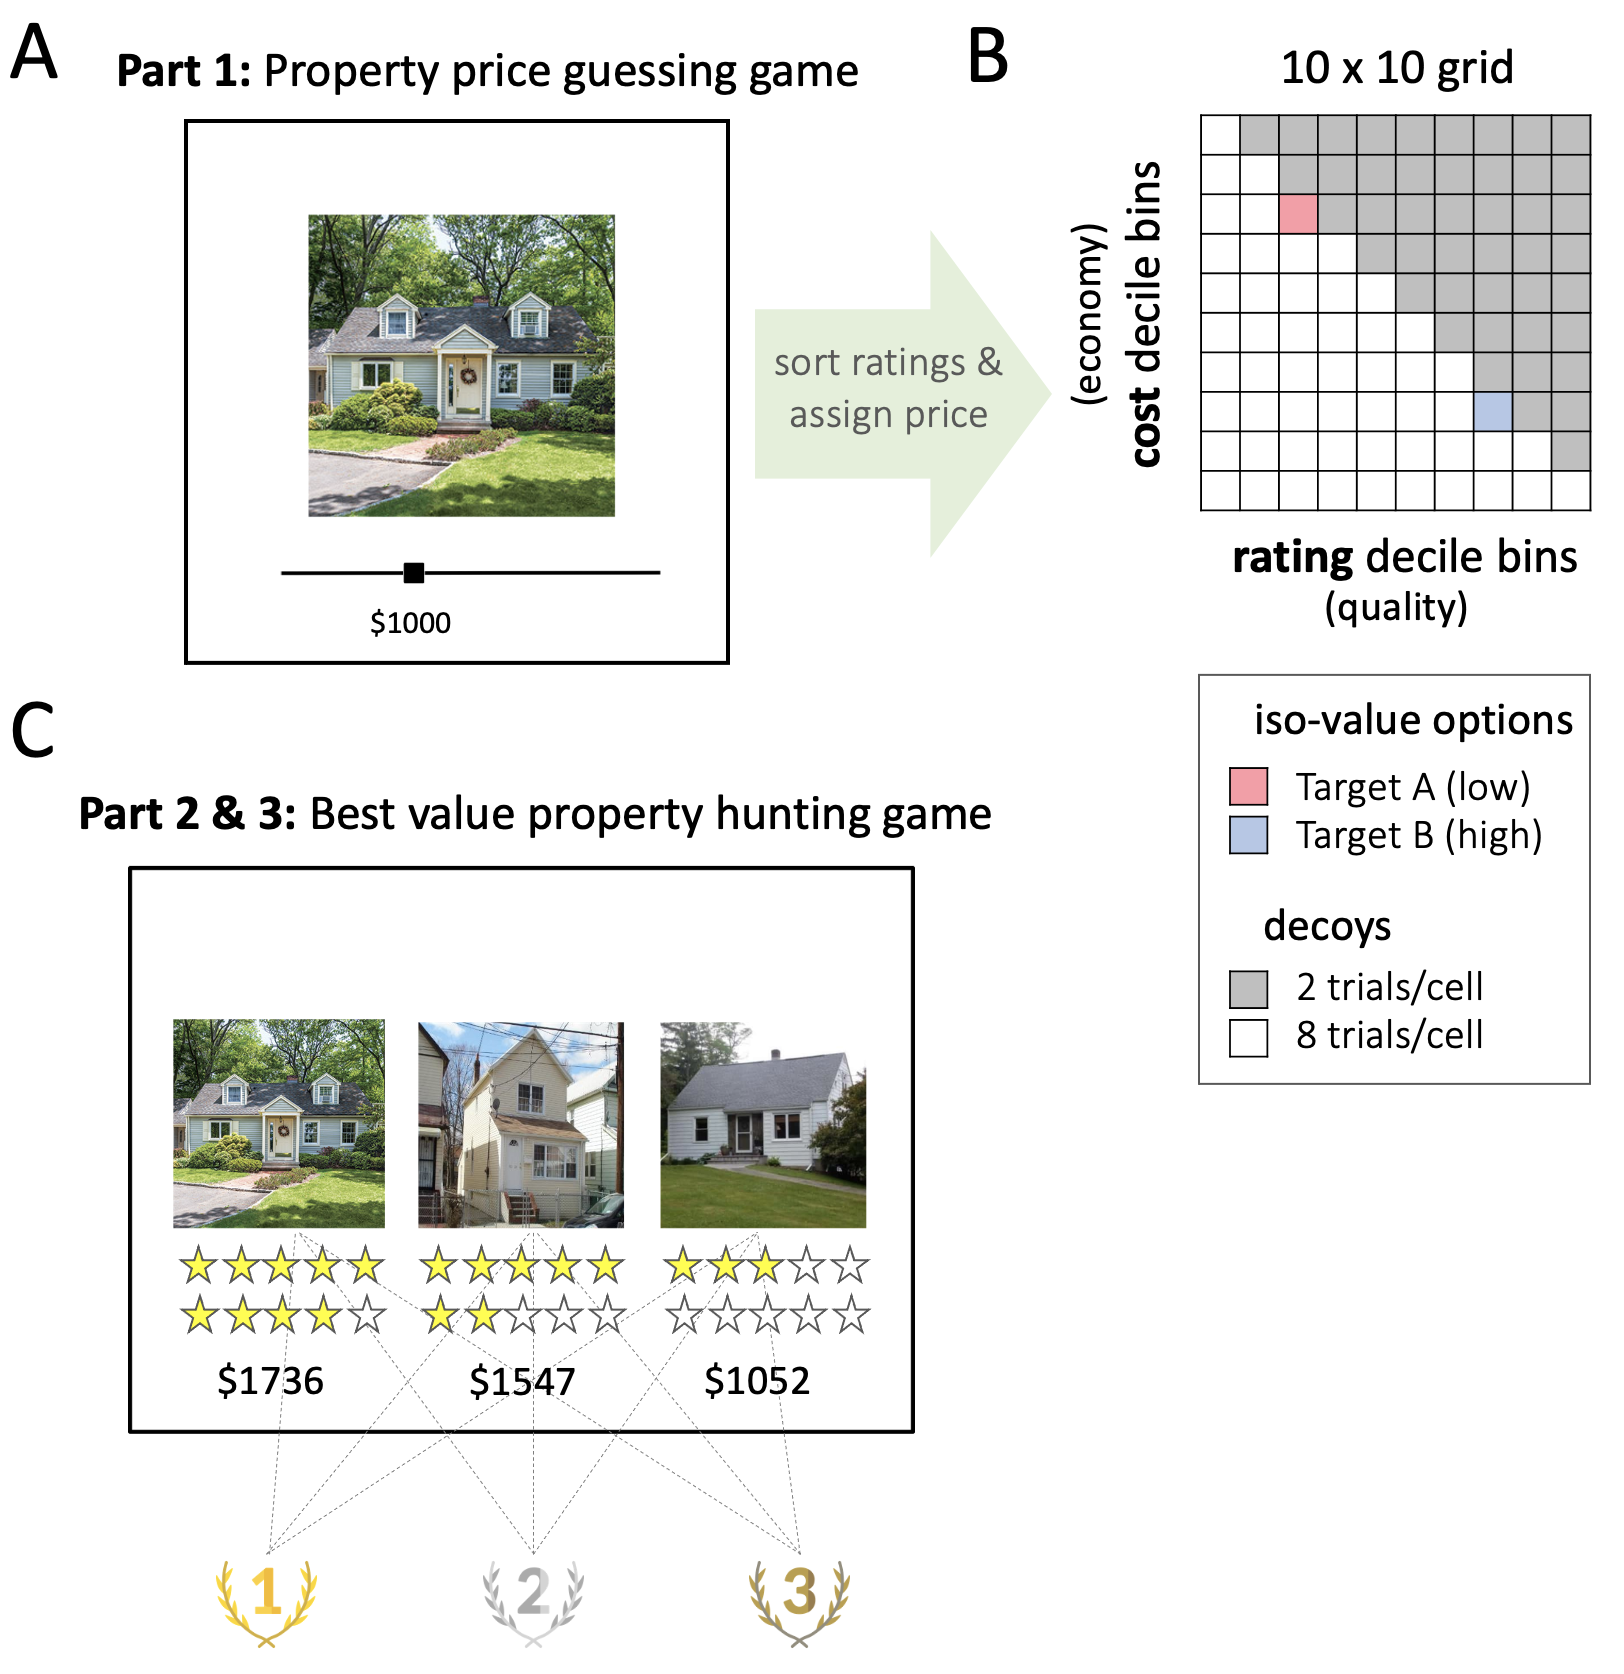
\includegraphics[width=0.9\linewidth]{figures/decoy-methods} 

}

\caption[Experimental design]{Experimental design. $\textbf{A:}$ Participants first played a “property price guessing game”.  On each trial they estimated the monthly rental value (in dollars) of a residential property, using a sliding scale. $\textbf{B:}$ After discarding properties with inconsistent responses, ratings were sorted into deciles for each participant. These bins were used to select stimuli for targets A and B (deciles 3 and 8 of estimated ratings; red and blue squares), and decoy stimuli. Each choice task stimulus was created by matching a property with a given decile estimated value (quality; attribute $j$) to a new rental price (economy; attribute $i$) on a 10x10 grid. Eight property/price combinations were generated for each cell in the grid that lay below the diagonal (white cells), and 2 property/price combinations for each cell above the diagonal (grey cells). $\textbf{C:}$ Participants then played a “best value property hunting game” in which they were asked to rank 3 stimuli according to their economy/quality trade off. Two of the stimuli corresponded to the targets A and B, the third stimulus was the decoy. A star rating system was used as a reminder of their previous price estimation judgment.}\label{fig:decoy-methods}
\end{figure}

\hypertarget{choice-task}{%
\paragraph{Choice Task}\label{choice-task}}

We introduced phases 2 and 3 as a ``best-value property hunting game'' (choice task, Fig. \ref{fig:decoy-methods}c). Here, participants were told to imagine that they were a real estate agent recommending to a client the best value house we, a fictitious real estate company, have on offer. On each trial, 3 properties (i.e.~choice alternatives) were displayed for a maximum of 60 seconds on left, central and right positions on the screen. Underneath each image we displayed an allocated rental cost (in dollars) and a number of stars. The number of stars was proportional to the value given by the participant in the ratings task, and merely served as a reminder. In piloting, we found that this improved choice consistency. Participants were informed that the property images were a subset of those that they had viewed in phase 1, and that that the stars were related to the ratings they themselves had reported. The task asked participants to press three keyboard buttons (left, down, and right arrow buttons) to indicate their ordered preference from the best-valued house to the worst-valued house. Participants were explicitly instructed that the best-valued house was the one with the highest market value but the lowest allocated rental price. At the end of each block, participants were told how many trials' recommendations were correct, given their initial ratings. The bonus payment at the end of each phase was proportional to their accuracy.

Unbeknownst to participants, the options were carefully selected for each participant individually to allow us to test our hypotheses of interest (Fig. \ref{fig:decoy-methods}b). First, for each participant we filtered out the 90 properties with the highest rating variability, i.e.~the highest absolute deviance between the two ratings. Second, the remaining 160 properties were binned into quality deciles (attribute \(i\)) on the basis of each participant's ratings. The binned properties could then be associated with an allocated rental cost that was drawn uniformly from within the range of dollar values that defined each decile (attribute \(j\)). This allowed us to select, on each trial, three stimuli that differed on two dimensions: two targets A and B, and a decoy stimulus. Target A was always a property drawn from the 3rd decile of quality (i.e.~participant rating) and the 8th decile of economy (i.e.~the 3rd decile of cost); target B was always drawn from the 8th decile of quality and the 3rd decile of economy (i.e.~the 8th decile of cost). The decoy stimulus was sampled exhaustively from the full attribute space (any of the 10 quality x 10 economy bins). Thus, targets A and B were equally valued options (A being low quality and low cost, and B being high quality and high cost) and the decoy stimulus could be both superior or inferior in value. Participants completed a total of 530 trials in the second part of the study. The third part constituted an additional 530 trials of the same task.

\hypertarget{analyses}{%
\subsubsection{Analyses}\label{analyses}}

We calculated relative choice share for the ``low'' item A over the ``high'' item B by calculating the proportion of trials for which A was chosen before B across all trials in each decoy decile bin. We were able to do this for both inferior and superior decoys, as participants provided us with ranked preference for all three items. Thus, even if on a given trial they chose the decoy, they still reported whether they preferred A over B or vice-versa. This allowed us to plot the relative preference for A over B across the full attribute space (\(RCS_{ij}\)).

\hypertarget{conventional-decoy-analyses}{%
\paragraph{Conventional Decoy Analyses}\label{conventional-decoy-analyses}}

We first adopted a standard approach from previous studies that have focused on estimating the effects of the three classic decoy effects, that is, calculating RCS for \(D_a\), \(D_c\) and \(D_s\). To this end, we defined portions of the influence map that corresponded to the traditionally defined positions of attraction, compromise and similarity decoys (Fig. \ref{fig:decoy-classic}a). We also included an additional decoy set that we called ``repulsion'' decoys (\(D_r\)): these were mirror-symmetric to the attraction decoys but located in the upper triangle of the influence map where the decoy was the objectively best option (i.e.~a set of ``superior'' decoys). We then calculated the RCS for \(D_a\), \(D_c\), \(D_s\) and \(D_r\), each defined with respect to target A and target B. The strength of each effect was defined as the difference in RCS for each decoy set defined with respect to targets A and B. We tested each effect against zero for statistical significance via a single sample \(t\) test.

\hypertarget{interrelationship-of-effects}{%
\paragraph{Interrelationship of Effects}\label{interrelationship-of-effects}}

To investigate the associations between the three classic decoy effects in our cohort, we calculated Pearson's correlation coefficients. We estimated those pairwise for each of the three possible combinations of effects (\(D_c\)-\(D_a\), \(D_c\)-\(D_s\), and \(D_a\)-\(D_s\)), based on the strength of the effects for each participant in our sample.

\hypertarget{map-of-decoy-influence}{%
\paragraph{Map of Decoy Influence}\label{map-of-decoy-influence}}

Our major goal for this project was to go beyond conventional analyses and chart decoy influence across the attribute space. The ordered RCS for option A over B in each decoy decile bin across all possible attribute combinations constitutes the map of decoy influence. In addition to the decoy map, as a sanity check, we also plotted preferences for the two targets \emph{over} the decoy item. We did this by calculating the RCS for option A over the decoy D (i.e.~in what proportion of trials did the participant choose A before D?), as well as the RCS for option B over the decoy D in each of the 10x10 decoy decile bins.

\hypertarget{map-decomposition}{%
\paragraph{Map Decomposition}\label{map-decomposition}}

The resulting map of decoy influence allowed us to not only ask how the three classic decoy effects are interrelated in our cohort of participants, but to seek structure beyond these three locations in attribute space. Using an exhaustive range of decoy locations allowed us to use dimensionality reduction approaches to examine the (potentially distinct) factors from which the map of decoy influence is composed. We used singular value decomposition (SVD) to identify factors contributing to the map of preference for A \textgreater{} B and calculate the variance explained by these factors. To this end, we flattened the 10x10 decoy map for each participant into a vector of values and constructed a large matrix of RCS, where each row indexed an individual participant and each column -- the decoy location in attribute space. SVD produces a set of basis functions, or factors, and allows us to examine the amount of variance explained by them in the empirical data. This, in turn, illustrates the structure of decoy effects across participants. Knowing this structure can give us clues as to whether distinct mechanisms drive decoy influence across different locations in attribute space, or alternatively, if the general structure of RCS can be explained by a single factor.

\hypertarget{data-code-availability-statement}{%
\subsubsection{Data \& Code Availability Statement}\label{data-code-availability-statement}}

All data and code to reproduce the analyses are available in the OSF repository (\url{https://osf.io/u6br3/}) for this project.

\hypertarget{results}{%
\subsection{Results}\label{results}}

\hypertarget{conventional-decoy-analyses-1}{%
\subsubsection{Conventional Decoy Analyses}\label{conventional-decoy-analyses-1}}

\begin{figure}

{\centering 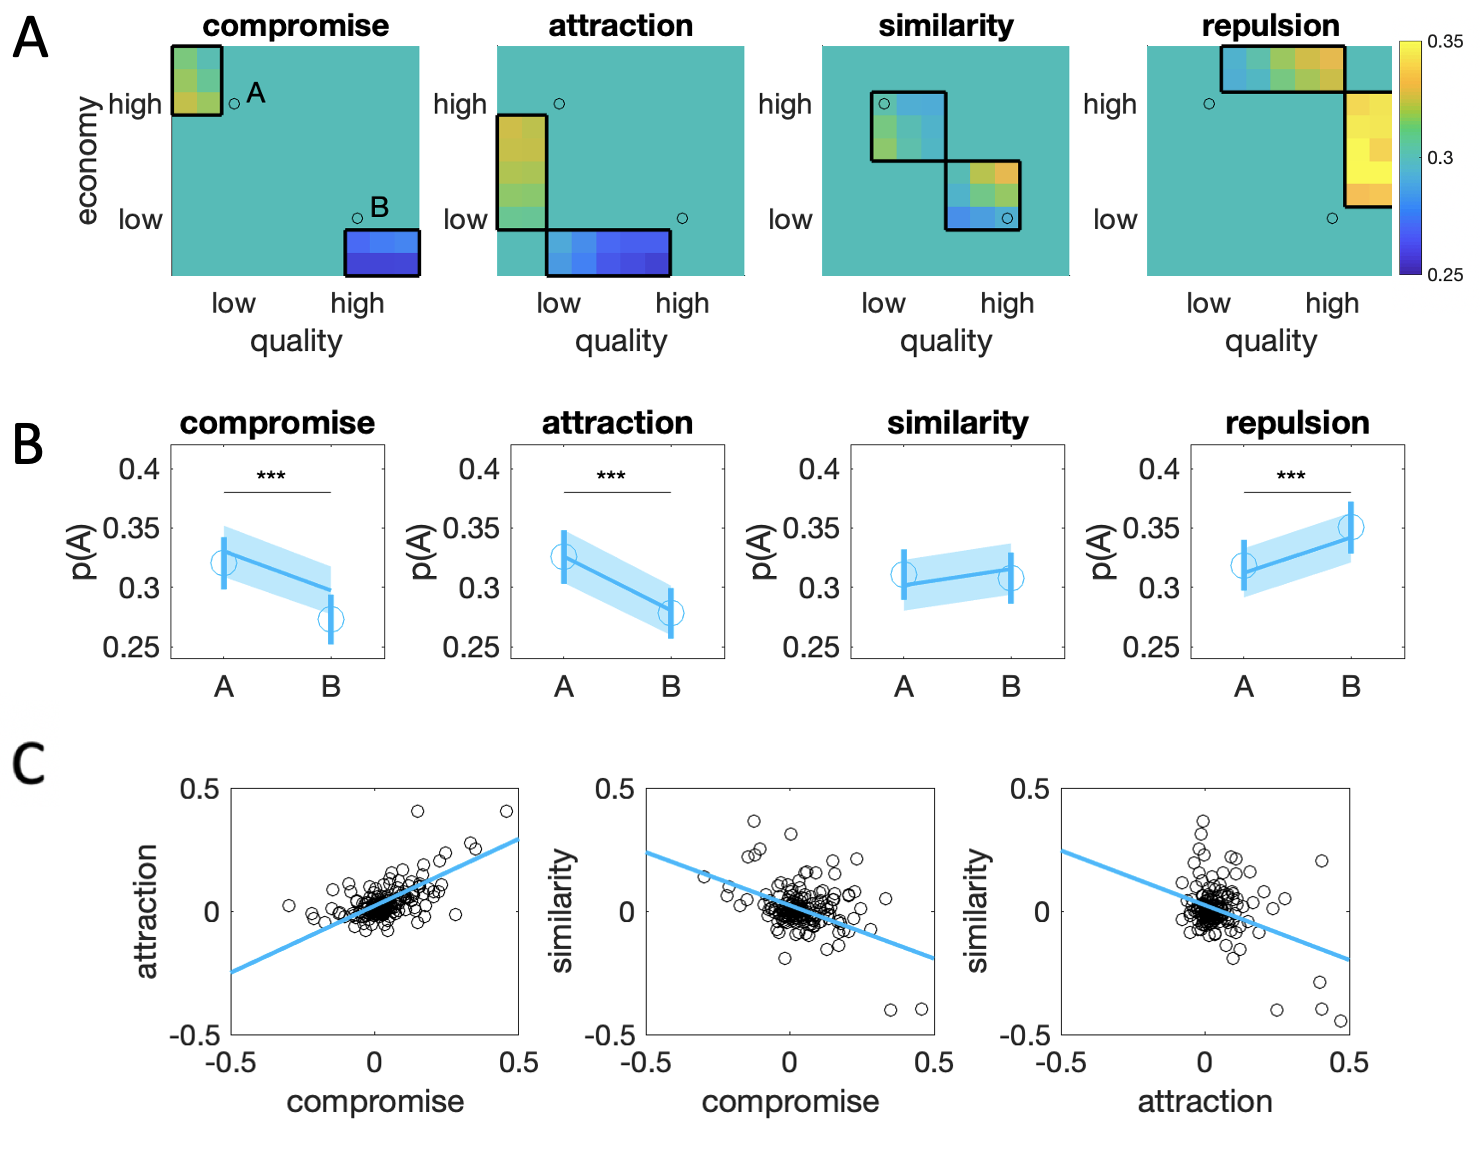
\includegraphics[width=1\linewidth]{figures/decoy-classic} 

}

\caption[Conventional decoy analyses]{Conventional decoy analyses. $\textbf{A:}$ Each panel illustrates the chosen locations in decoy space for compromise ($D_c$), attraction ($D_a$), similarity ($D_s$) and repulsion ($D_r$) decoys (boxes). The blue-yellow color scale illustrates relative preference for target A over B (warmer colors) or vice versa (colder colors) at each location. Black circles indicate the locations of targets A and B.  $\textbf{B:}$ Average choice share for target A as a function of decoy location across $D_c$, $D_a$, $D_s$ and $D_r$. Blue dots are human data, shaded lines are model fit of adaptive gain model (see below). Bars/shaded area signal M±SEM *** indicates p < 0.001. $\textbf{C:}$ Correlations between the attraction, compromise and similarity effects. Each dot is a single participant; the decoy estimate is calculated as the difference between the RCS for given decoy with respect to targets A and B. }\label{fig:decoy-classic}
\end{figure}

Fig. \ref{fig:decoy-classic}b illustrates the difference in choice share driven by decoys in the 4 locations associated with \(D_c\), \(D_a\), \(D_s\) and \(D_r\) (defined in Fig. \ref{fig:decoy-classic}a). As a first general observation, despite the careful sampling of targets that were matched in price/quality ratio according to participants' responses in the valuation phase, and despite the incentives offered for consistent responding, participants exhibited a bias towards the high item B (average RCS \textasciitilde{} 0.7) over the low item A. Despite this additive bias, however, decoys had a clear and robust influence on choice. Participants exhibited clear attraction (\(t_{188}=4.74\), \(p<0.001\)) and compromise (\(t_{188}=6.31, p<0.001\)) effects, which were statistically significant and in the expected direction. There was also empirical support for a repulsion effect (\(t_{188}=3.45\), \(p<0.001\)) from superior decoys. On average, the presence of attraction, compromise or repulsion decoys shifted preferences from A to B by about 3-5\%. However, we failed to replicate the similarity decoy effect (\(t_{188}=0.41\), \(p = 0.68\)).

\hypertarget{interrelationship-of-effects-1}{%
\paragraph{Interrelationship of Effects}\label{interrelationship-of-effects-1}}

We observed a positive association between the attraction and compromise effects (\(r=0.72\), \(p<0.001\)) and a negative relation between the similarity effect and both compromise (\(r=-0.59\), \(p<0.001\)) and attraction (\(r=-0.46\), \(p<0.001\)) effects. Note that the latter correlations were observed despite the fact that in our data, the similarity effect was on average non-significant. These are shown in Fig. \ref{fig:decoy-classic}c.

\hypertarget{map-of-decoy-influence-1}{%
\paragraph{Map of Decoy Influence}\label{map-of-decoy-influence-1}}

\begin{figure}

{\centering 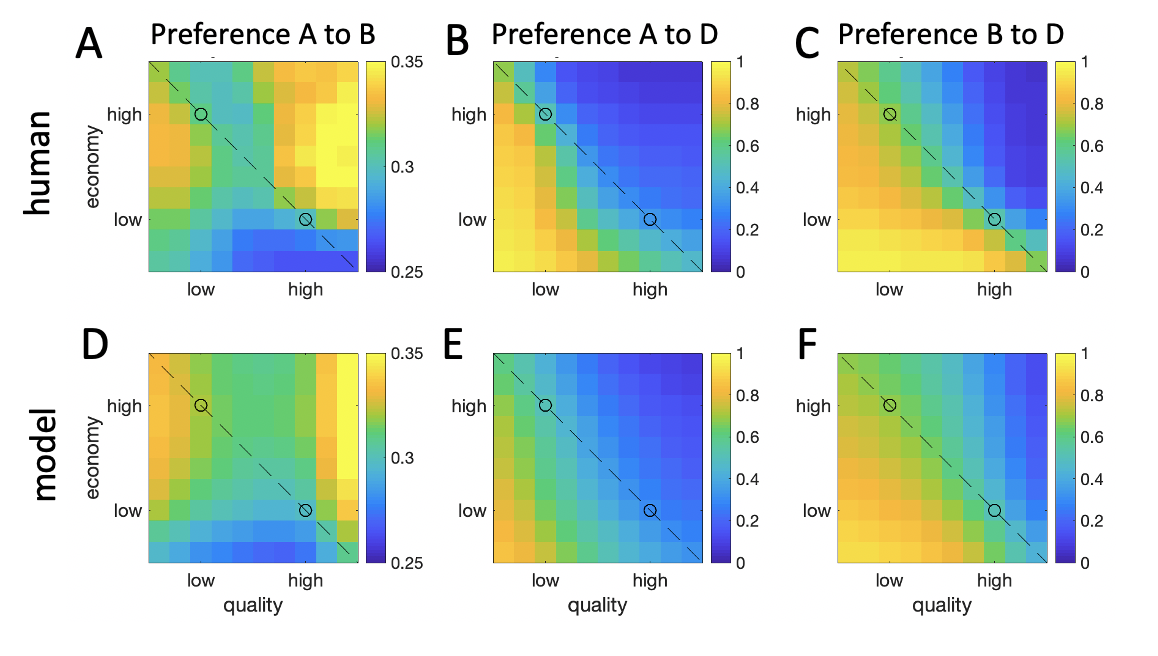
\includegraphics[width=1\linewidth]{figures/decoy-map} 

}

\caption[Map of decoy influence]{Map of decoy influence. $\textbf{A:}$ Decoy influence map showing $RCS_{ij}$ for A over B (left panels), A over D (middle panels) and B over D (right panels). Upper plots are the human data and lower plots are the same data for the simulated adaptive gain model (see below). The dashed line signals isopreference and the black circles are the targets A and B.}\label{fig:decoy-map}
\end{figure}

The full map of decoy influence \(RCS_{ij}\) is shown in Fig. \ref{fig:decoy-map}a. Visual inspection reveals that the map has rich structure beyond the traditional decoy locations. Relative preferences for A and B seem to be driven by a dynamic of attraction and repulsion that depends on the position of the decoy with respect to each target stimulus. Robust attraction effects (whereby the presence of a decoy that is dominated by A shifts preferences towards A) were mirrored by strong repulsion effects (whereby a decoy that dominates A shifts preferences towards B). Attraction and repulsion were observed for both targets in approximate symmetry.

The map charting preference for A \textgreater{} D (Fig. \ref{fig:decoy-map}b) is in line with the expected pattern, whereby inferior decoys, i.e.~those under the left diagonal, or line of theoretical isopreference, are chosen less often (warmer colors) than superior decoys (colder colors). Similarly, the map charting preference for B \textgreater{} D (Fig. \ref{fig:decoy-map}c) adheres to this general pattern. In theory, if A and B were equally preferred, these two maps would be identical. However, in line with the observed preference bias for the high value item B, we see that overall, preferences for A \textgreater{} D appear weaker compared to preferences for B \textgreater{} D.

\hypertarget{map-decomposition-1}{%
\paragraph{Map Decomposition}\label{map-decomposition-1}}

\begin{figure}

{\centering 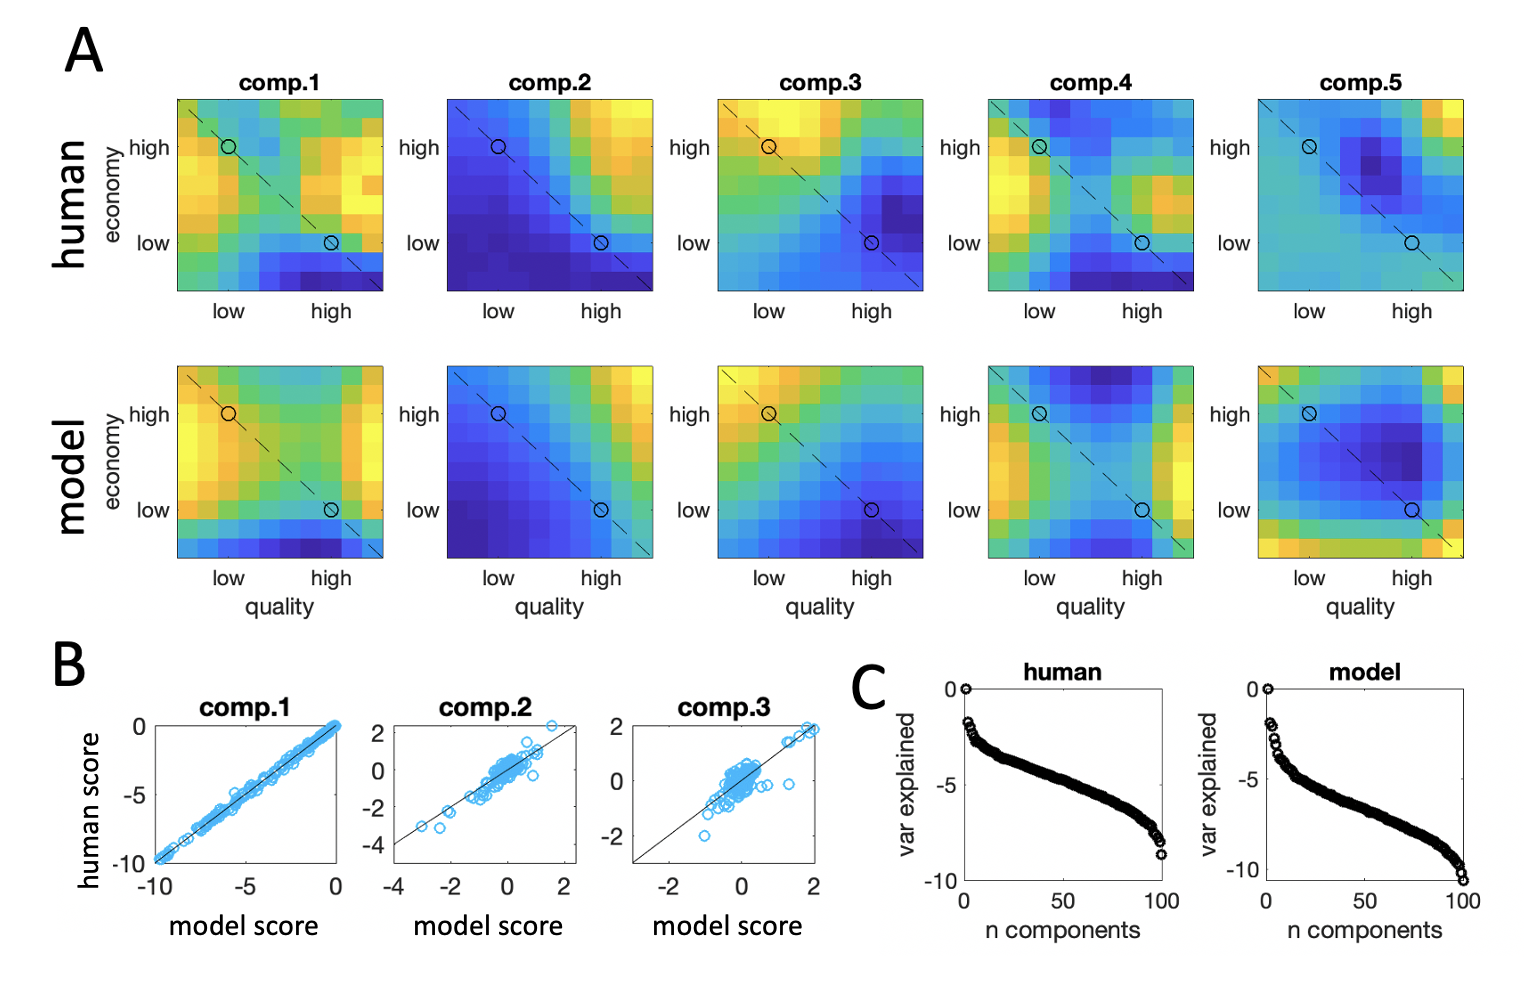
\includegraphics[width=1\linewidth]{figures/decoy-svd} 

}

\caption[Map decomposition]{Map decomposition. $\textbf{A:}$ First five components obtained from singular value decomposition (SVD) of the RCS for A vs. B. Upper plots are the human data and lower plots are the model. $\textbf{B:}$ Correlation between component scores for components 1-3 between the human and the best-fitting model. For components 1-3, this correlation was very high. $\textbf{C:}$ The variance explained by each component obtained by SVD for the humans (left panel) and the model (right panel). Note that the y-axis is on a log scale; the data is dominated by the first component in both cases.}\label{fig:decoy-svd}
\end{figure}

Next, we sought to examine the structure of the map of decoy influence (Fig. \ref{fig:decoy-map}a) via dimensionality reduction. The first 5 factors identified by SVD are visualized in Fig. \ref{fig:decoy-svd}a (top row). The first factor accounted for 95\% of the variance in the data, suggesting that there is a single explanatory variable that drives decoy effects across participants (Fig. \ref{fig:decoy-svd}c, right panel, note the logarithmic scale on the y-axis). This finding is consistent with the correlation results reported above, showing the robust interrelationships between the three classic effects in our participants.

\hypertarget{interim-discussion}{%
\subsection{Interim Discussion}\label{interim-discussion}}

Conventional decoy analyses of our data replicated the previously extensively documented compromise and attraction effects \autocite{huber1982,simonson1989}. However, we failed to replicate the similarity decoy effect in this dataset, consistent with weak or absent similarity effect from other studies \autocite{noguchi2014,berkowitsch2014}. Indeed, while the attraction effect tends to be highly robust and consistent across participants, the compromise effect and similarity effects tend to be more idiosyncratic, with a high proportion of participants showing effects which are inverted with respect to the canonical form. For example, in previous studies only a minority of participants show all three effects (numerically) in the expected direction \autocite[e.g.~only 23\% in][we find a comparable figure of 22\%]{trueblood2015}.

Despite the fact that the similarity effect was on average non-significant in our dataset, its strength inversely correlated with the strength of the compromise and attraction effects. Those two effects were in turn positively associated with one another. This pattern of interrelationships of the decoy effects mirrors previous reports \autocite{noguchi2014} and is further supported by our results on the structure of the full map of decoy influence. In particular, we found that a single explanatory factor is sufficient to capture 95\% of the variability of decoy influence in our dataset.

One interpretation of this data is that the attraction, compromise and similarity effects are not distinct phenomena, but rather they are all driven by a single common computational principle. This principle ensures that decision values of stimuli A and B are repulsed away from proximal decoys on a line which lies perpendicular to the line of isopreference, giving rise firstly to what is traditionally known as the ``attraction'' effect (a potentially confusing nomenclature, given that decision values for a target are repulsed away from those of the decoy) and secondly to its converse identified here for superior decoys, which we have dubbed the ``repulsion'' effect. The compromise and similarity effects can arise because these repulsive effects may vary in strength for targets A and B, and/or for inferior and superior decoys, such that repulsive effects ``spill over'' asymmetrically towards the extremes of the isopreference line (compromise effect) or into the center of the bivariate decoy map (similarity effect). It is the fact that compromise and similarity effects are really driven by asymmetric attraction and repulsion that gives rise to the strong correlations in effects across the cohort observed in this paper and previously \autocite{berkowitsch2014}.

\hypertarget{computational-modeling}{%
\section{Computational Modeling}\label{computational-modeling}}

These findings suggest that it should be possible to identify a simple model that can reproduce the full decoy influence map with parameters that control the putative repulsive principle, as well as additional degrees of freedom that allow for asymmetric scaling of the attribute values (quality and economy). Previous simulation work demonstrated that a gain-control process can provide a unifying explanation for similar choice biases \autocite{li2018}. In this theoretic account, the gain with which alternatives are encoded is adaptively adjusted according to the context provided by other available options. Recent proposals of models for decoy phenomena have also appealed to a similar adaptive framework, whereby decision signals are normalized by context \autocite{rigoli2017,daviet2018}.

\hypertarget{adaptive-gain-model}{%
\subsection{Adaptive Gain Model}\label{adaptive-gain-model}}

The normalization principle in the adaptive gain model assumes that for each attribute (e.g.~quality or economy), a \emph{relative} value estimate is computed that reflects the distance between each item and the mean of the available choice set. We thus begin by defining \(r(A)\), which is the value of target A relative to other items, including the decoy, on a given attribute \(i\):
\begin{equation}
r(A_i) = v(A_i) - v(avg_i^{ABD})
\label{eq:decoy-ag-r}
\end{equation}
where \(v(avg_i^{ABD})\) corresponds to the average value of the three alternatives on attribute \(i\):
\begin{equation}
v(avg_i^{ABD})=\frac{v(A_i)+v(B_i)+v(D_i)}{3}
\end{equation}
The model proposes that the subjective utility \(u(A_i)\) of target A on attribute \(i\) is computed through a logistic transformation of the relative value, as follows:
\begin{equation}
u_i(A_i) = \frac{1}{1+e^{-(r(A_i)-c_i)\cdot s^{-1}}}
\label{eq:decoy-ag}
\end{equation}
Thus, for each attribute, the utility of each target is given by a logistic function with slope \(s\) whose inflection point is the mean value of all items plus an additive bias term \(c\). The additive bias \(c\) can potentially vary across attributes.

The utility of target A is a weighed sum of its attributes \(i\) and \(j\), and the final decision is made by passing the utilities of all three rival stimuli through a softmax function to make a ternary choice:
\begin{equation}
u(A) = w \cdot u_i(A_i) + (1-w) \cdot u_j(A_j)
\label{eq:decoy-item-u}
\end{equation}
\begin{equation}
p(A) = \frac{e^{\tau u(A)}}{e^{\tau u(A)}+e^{\tau u(B)}+e^{\tau u(D)}}
\label{eq:decoy-prob}
\end{equation}
In addition to the softmax temperature \(\tau\), the model potentially has 4 free parameters of interest: the slope \(s\), and inflection points \(c_i\) and \(c_j\) of the logistic function Eq. \eqref{eq:decoy-item-u}, and the weighing parameter \(w\) in Eq. \eqref{eq:decoy-prob}.

\begin{figure}

{\centering 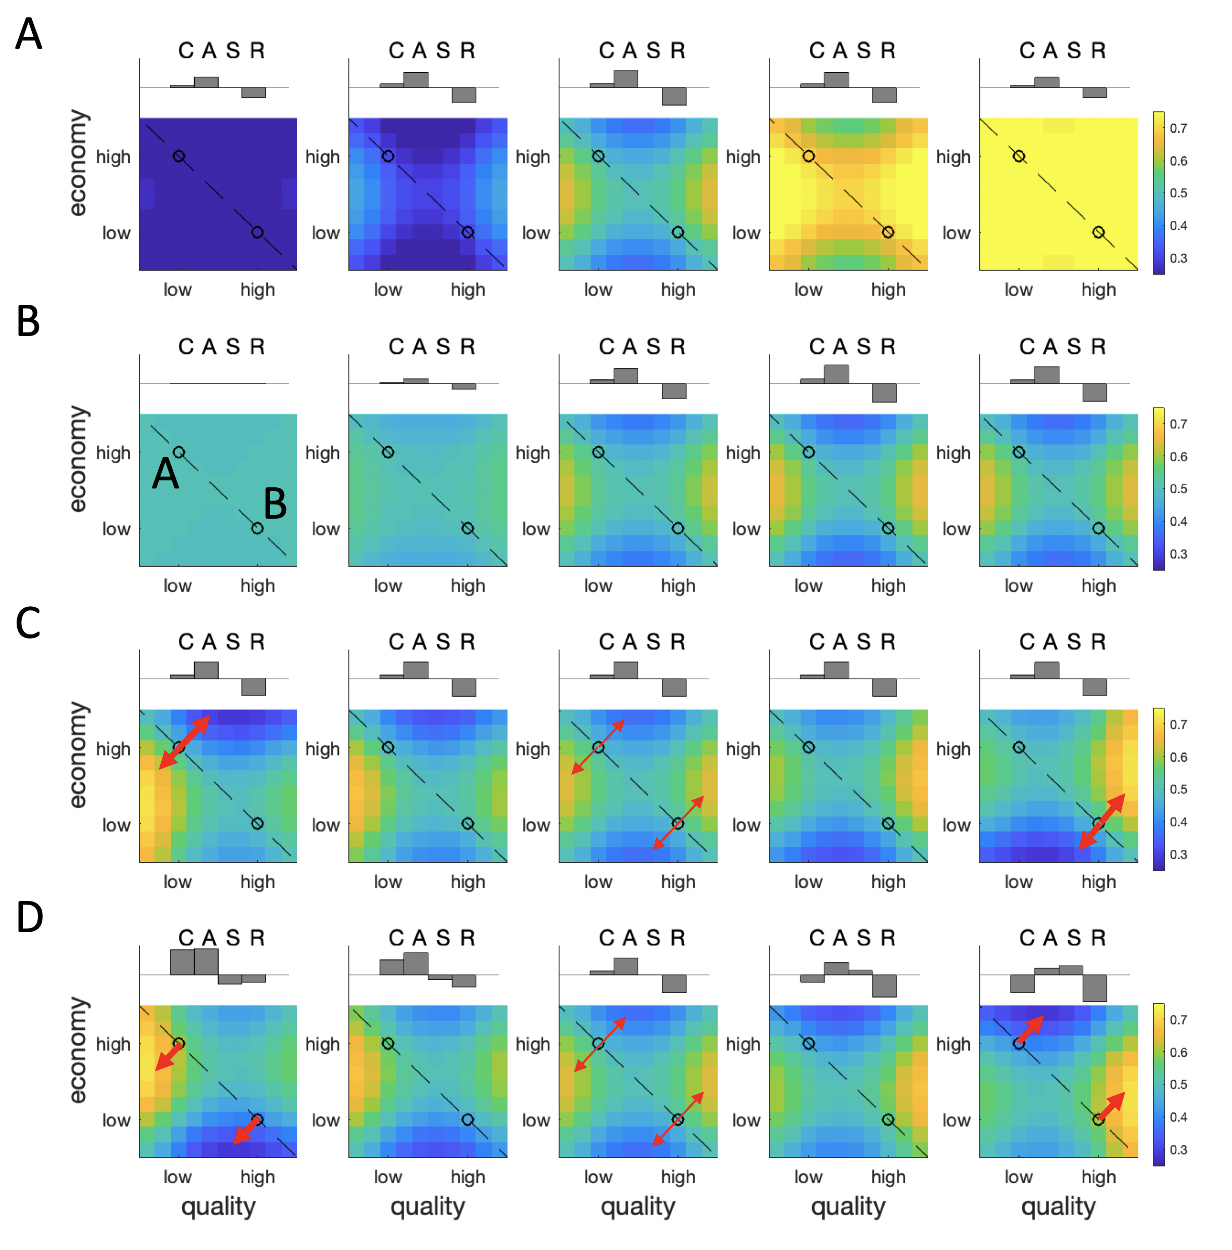
\includegraphics[width=1\linewidth]{figures/decoy-sim} 

}

\caption[Map simulations]{Simulated maps of decoy influence. $\textbf{A:}$ Effect of varying the parameter $w$ from low (left panels) to high (right panels). This parameter controls the relative preference for low price/quality to high price/quality items. $\textbf{B:}$ The effect of varying the parameter $s$ from high to low. This parameter controls whether A and B are equally preferred, or whether there is decoy-like distortion. $\textbf{C:}$  The effect of varying the difference of bias terms $c_i$=$-c_j$ from negative (left panels) to positive (right panels). Varying this difference alters whether the maximal distortion occurs proximal to target A (left) or target B (right). $\textbf{D:}$ The effect of varying the sum of bias terms $c_i=c_j$ from negative (left panels) to positive (right panels). Varying this difference alters whether the maximal distortion occurs for inferior decoys (left) or superior decoys (right). Red arrows highlight directions of repulsion, with arrow width schematically representing the strength of the effect. }\label{fig:decoy-sim}
\end{figure}

\hypertarget{model-simulations}{%
\subsubsection{Model Simulations}\label{model-simulations}}

We explore the effects of manipulating these parameters on the predicted decoy influence map in Fig. \ref{fig:decoy-sim}; a full description of the parameters used is available in Table \ref{tab:decoy-table}. This figure shows how the model can systematically account for not only the pattern observed in the current experiment, but also those from previous (and potentially contradictory) reports. In Fig. \ref{fig:decoy-sim}a we show the effect of manipulating the parameter \(w\). This simply shows how we can tip the balance of preferring A over B according to the relative weight given to each attribute.

In Fig. \ref{fig:decoy-sim}b, with \(w\) now fixed to 0.5 (equal weighing of the two attributes), we show how the decoy effects grow in strength with \(s\). Above each plot the relative positive or negative strength of the compromise (\(D_c\)), attraction (\(D_a\)), similarity (\(D_s\)) and repulsion (\(D_r\)) effects are shown in a bar plot. As can be seen, the attraction and repulsion effects grow as \(s\) grows, including a weak compromise effect but no similarity effect.

Fig. \ref{fig:decoy-sim}c shows the influence of varying \(c_i=-(c_j)\) while \(s\) and \(w\) are fixed. This has the effect of shifting the relative strength of the attraction/repulsion effect for targets A and B. For example, when \(c_i>c_j\) the attraction/repulsion effects are strongest for the target A, whereas when \(c_j>c_i\) they are strongest for B (red arrows). However, because these effects cancel out symmetrically, this does not affect the overall RCS for \(D_c\), \(D_a\), \(D_s\) or \(D_r\).

Finally, varying \(c_i=c_j\) (Fig. \ref{fig:decoy-sim}d) brings about an asymmetric distortion whereby either attraction effects are stronger (i.e.~below the isopreference line) or repulsion effects are stronger (in the superior decoy portion of space). In addition to varying the relative strength of attraction and repulsion, this allows the compromise effect to vary from positive to negative, as described in previous studies; it allows a weak similarity effect to emerge. Combinations of all of these factors give the model systematic flexibility to account for a wide range of observed effects.

\begin{table}

\caption{\label{tab:decoy-table}Parameters for map simulation.}
\centering
\resizebox{\linewidth}{!}{
\begin{tabular}[t]{lllllll}
\toprule
Panel & Constants & Column 1 & Column 2 & Column 3 & Column 4 & Column 5\\
\midrule
A & s=0.1; $\tau=0.1$ & $w=0.4$ & $w=0.45$ & $w=0.5$ & $w=0.55$ & $w=0.6$\\
 & $c_i=0$; $c_j=0$ &  &  &  &  & \\
B & $w=0.5$; $\tau=0.1$ & $s=0.01$ & $s=0.0325$ & $s=0.055$ & $s=0.0775$ & $s=0.1$\\
 & $c_i=0$; $c_j=0$ &  &  &  &  & \\
C & $w=0.5$; $\tau=0.1$ & $c_i=-0.04$ & $c_i=-0.02$ & $c_i=0$ & $c_i=0.02$ & $c_i=0.04$\\
\addlinespace
 & $s=0.1$ & $c_j=0.04$ & $c_j=0.02$ & $c_j=0$ & $c_j=-0.02$ & $c_j=-0.04$\\
D & $w=0.5$; $\tau=0.1$ & $c_i=-0.04$ & $c_i=-0.02$ & $c_i=0$ & $c_i=0.02$ & $c_i=0.04$\\
 & $s=0.1$ & $c_j=-0.04$ & $c_j=-0.02$ & $c_j=0$ & $c_j=0.02$ & $c_j=0.04$\\
\bottomrule
\end{tabular}}
\end{table}

Interestingly, the simulations shown in Fig. \ref{fig:decoy-sim}d allow us to make a new prediction about the human data. As seen in the bar plots accompanying each predicted influence map, when \(c_i\) and \(c_j\) are both negative, the compromise effect is positive and attraction is stronger than repulsion. By contrast, when \(c_i\) and \(c_j\) are both positive, the compromise effect is negative and the repulsion effect is stronger than attraction. The model thus predicts that on average, in the human data there will be a correlation between the (signed) compromise effect and the relative magnitude of attraction vs repulsion. This is plotted in Fig. \ref{fig:decoy-new-rel}, and as can be seen this prediction holds for the data we collected (\(r=0.57\), \(p<0.001\)). Of note, this effect was driven both by a positive correlation between the compromise effect and the strength of repulsion (\(r=0.43\), \(p<0.001\)), as well as the correlation between compromise and attraction effects described above.

\begin{figure}

{\centering 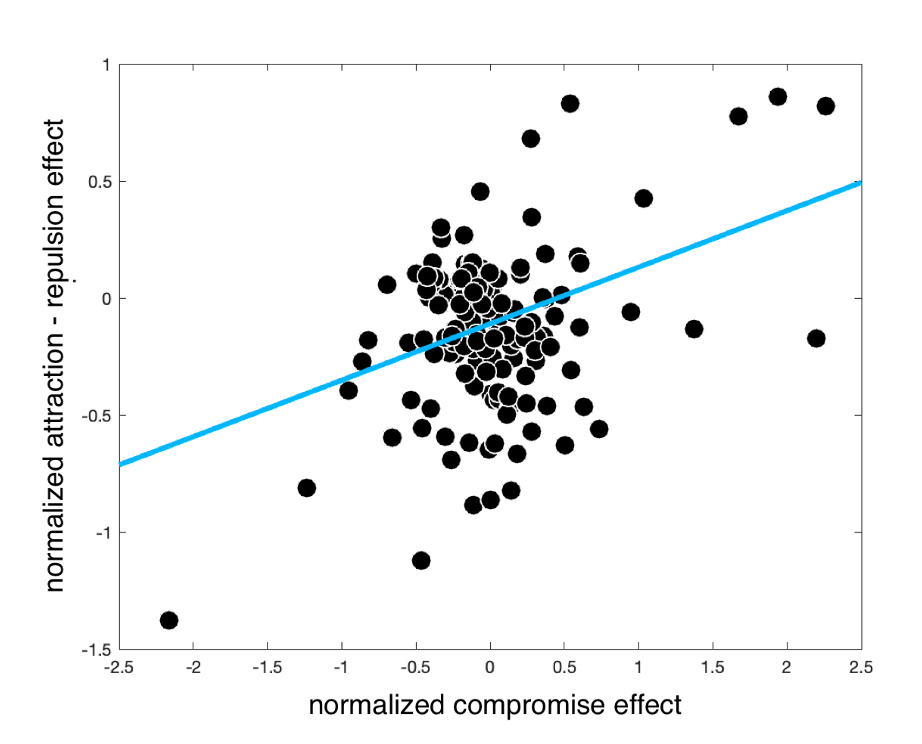
\includegraphics[width=0.5\linewidth]{figures/decoy-new-rel} 

}

\caption[New decoy relationship]{Correlation between the compromise effect and the relative strength of attraction vs repulsion in the human data.  Each dot is a participant; the blue line is the best fitting linear trend.}\label{fig:decoy-new-rel}
\end{figure}

\hypertarget{model-fitting}{%
\subsubsection{Model Fitting}\label{model-fitting}}

Next, we estimated the model parameters which best fit the data for each participant in our experiment to assess whether the model was able to capture the results at the individual as well as aggregate level.

\hypertarget{model-fitting-methods}{%
\paragraph{Model Fitting Methods}\label{model-fitting-methods}}

The model provided predictions about probabilities of choosing option A over B, which allowed us to compute model likelihoods on each trial. Those likelihoods were then used for model fitting and comparison. We estimated the model for each participant individually using gradient descent with the \texttt{globalsearch} function from the MATLAB Optimization Toolbox.

\hypertarget{model-fitting-results}{%
\paragraph{Model Fitting Results}\label{model-fitting-results}}

Fitting this 5-parameter (\(\tau\), \(s\), \(c_i\), \(c_j\), \(w\)) model to human data, we can fully recreate the decoy effects observed in this study using both conventional (Fig. \ref{fig:decoy-classic}b) and novel (Fig. \ref{fig:decoy-map}d-f) analysis methods. Specifically, the model captured almost exactly the pattern of traditional decoy effects, in terms of the relative impact on RCS of \(D_a\), \(D_c\) and \(D_s\), as well as the repulsion decoy \(D_r\) (blue shaded lines in Fig. \ref{fig:decoy-classic}b). The model reproduced the pattern of preferences for target A \textgreater{} target B qualitatively and quantitatively across the decoy space, and when we applied SVD to the model data generated under the best-fitting parametrization for each participant, the first five components that emerged were nearly identical to those for humans, and the first model component explaining 97\% of the variance (Fig. \ref{fig:decoy-svd}c). When we plotted the estimated singular values for the first three components for humans and the best-fitting model, we found them to be very tightly correlated (Fig. \ref{fig:decoy-svd}b). The model also displayed the same pattern of positive association between attraction and compromise effect (\(r=0.86\)) and negative association between the similarity and attraction (\(r=-0.85\)) and similarity and compromise effects (\(r=-0.94\)). In other words, the model captures the human data very closely, both at the individual and the aggregate level.

\hypertarget{model-comparisons}{%
\subsection{Model Comparisons}\label{model-comparisons}}

The adaptive gain model belongs to a class of models which describe contextual biases as arising from normalization among populations of neurons. Normalization models share commitment to the idea that information is divisively normalized by the local context. The precise mathematical formulation of this procedure, however, differs between theoretical accounts. Some models, for instance, use measures of the central tendency of the features present in the local context \autocite[e.g.~the average of attribute values,][]{louie2013}, while other appeal to measures of the dispersion of features \autocite[e.g.~the range of attribute values,][]{soltani2012}. Similarly, models might encode features linearly \autocite[e.g.][]{bushong2021} or compress them prior to normalization \autocite[e.g.~via a logistic operation as in the model described here and in][]{rigoli2019}. Below we highlight several prominent normalization models in the literature. Our aim was to compare our model to a broad space of alternative accounts that similarly assume the value of each target (on each attribute) is encoded relative to its competitors. Thus, we began our model comparison exercise with contrasts with those well established competitors.

The classic formulation of the divisive normalization theoretical tradition (henceforth vanilla divisive normalization, VDN) can be broadly encapsulated in the following expression \autocite{carandini2012,louie2013}:
\begin{equation}
u_i(A_i)^{VDN} = \frac{v(A_i)}{v(avg_i^{ABD})+c_i}
\label{eq:decoy-vdn}
\end{equation}
where \(c_i\) is a small regularization constant. The model assumes that decision inputs are divided by the current contextual expectation, that is, the average of all current options.

In one variant of this model, which has been recently and successfully used to account for decoy effects, this normalization is also ``recurrent'', i.e.~it overweighs the focal item's contribution to normalization \autocite{daviet2018,webb2021}:
\begin{equation}
u_i(A_i)^{RDN} = \frac{v(A_i)}{v(A_i)+v(avg_i^{ABD})+c_i}
\label{eq:decoy-rdn}
\end{equation}

Note that the adaptive gain model (Eq. \eqref{eq:decoy-ag}) is equivalent to a form of the recurrent divisive normalization model in which the values are exponentiated prior to normalization:
\begin{equation}
u_i(A_i)^{AG} = \frac{\exp(\frac{v(A_i)}{s})}{\exp(\frac{v(A_i)}{s})+\exp(\frac{v(avg_i^{ABD})+c_i}{s})}
\label{eq:decoy-rdn}
\end{equation}

Alongside these two models, we also considered a class of contextual normalization, which uses the range (rather than the average) of attribute values being encoded on a given trial to normalize an imperative stimulus:
\begin{equation}
u_i(A_i)^{RN} = \beta \frac{v(A_i)}{v(rng_i^{ABD})}
\label{eq:decoy-rn}
\end{equation}
where \(v(rng_i^{ABD})\) corresponds to the corresponds to the difference between highest and lowest values of attribute \(i\) across all stimuli (target or decoy) in the trial and \(\beta\) is a scaling term \autocite{soltani2012,bushong2021}.

\hypertarget{methods-1}{%
\subsubsection{Methods}\label{methods-1}}

We compared the fit of each of the candidate normalization accounts to adaptive gain in a direct model comparison exercise. To achieve this, we used Bayesian model selection on cross-validated model evidence. Cross-validation involved estimating model parameters from one half of trials (by comparing fits to preferences between target items A and B, as well as preferences between target and decoys) and computing log-likelihoods from the held-out trials. We implemented this using the \texttt{globalsearch} function from the MATLAB Optimization Toolbox. For Bayesian model selection, we used the Statistical Parametric Mapping Toolbox \autocite{stephan2009}.

\hypertarget{results-1}{%
\subsubsection{Results}\label{results-1}}

Comparisons between cross-validated model likelihoods revealed that the exceedance probability for the adaptive gain model over each of the three competitor models (vanilla divisive normalization, recurrent divisive normalization and range normalization) was 0.99, providing decisive evidence for the former over each of the latter.

\hypertarget{charting-normalization-models-of-decoy-influence}{%
\subsection{Charting Normalization Models of Decoy Influence}\label{charting-normalization-models-of-decoy-influence}}

\hypertarget{grandmother-model}{%
\subsubsection{Grandmother Model}\label{grandmother-model}}

To go beyond those established models and compare our model to a broader range of competitors, we also devised and fit a more flexible model which encompassed a large space of possible normalization schemes. This ``grandmother'' model could capture the encoding scheme proposed by the 4 models introduced above, along with a number of other ``hybrid'' models. Thus, exploring the parameter space of the grandmother model allows us to explore the space of putative normalization schemes, including those that are yet to be described in the literature, and chart how different model features translate to predicted patterns of decoy influence.

The model had the general form:

\begin{equation}
u_i(A_i) = \frac{1}{\beta_1 + e^{-(v(A_i)^k - \mu_i^k)(s \cdot k)^{-1}}}
\label{eq:grandmother}
\end{equation}
where
\begin{equation}
\mu_i = c_i+ \beta_2  \cdot v(avg^{ABD}_i)+(1-\beta_2)\cdot v(rng^{ABD}_i)
\end{equation}

We focus on free parameters \(\beta_1\), \(\beta_2\), and \(k\), which respectively encode the tendency to engage in asymmetric weighing of the evaluated (recurrent) item (\(\beta_1\)), the tendency to normalize with respect to the mean vs range (\(\beta_2\)) and the extent to which inputs are compressed before being transduced (\(k\)).

Parameter \(k\) facilitated comparison between the adaptive gain model (which incorporates a logistic transformation) and other normalization models (which do not), by leveraging the following limit:

\begin{equation}
\lim_{k \to 0} \frac{x^k-1}{k} = \log_e x, \forall x>0 
\label{eq:decoy-limit}
\end{equation}

Thus, substituting \(x\) above for our variables of interest, \(v(A_i)\) and \(\mu\), we obtain:

\begin{equation}
\log v(A_i) - \log \mu_i = \lim_{k \to 0} \frac{v(A_i)^k-1}{k}-\frac{\mu_i^k-1}{k} = \lim_{k \to 0} \frac{v(A_i)^k - \mu_i^k}{k}
\label{eq:decoy-limit-eq}
\end{equation}

Thus, \(k\) thus corresponds to the extent to which inputs are compressed before being transduced, with \(k\sim 0\) signifying a logarithmic compression, and \(k=1\) signifying linear input. Simulations revealed that implementing a value of \(k\) as high as 0.001 satisfactorily approximates the natural logarithm (Fig. \ref{fig:decoy-log}).

\begin{figure}

{\centering 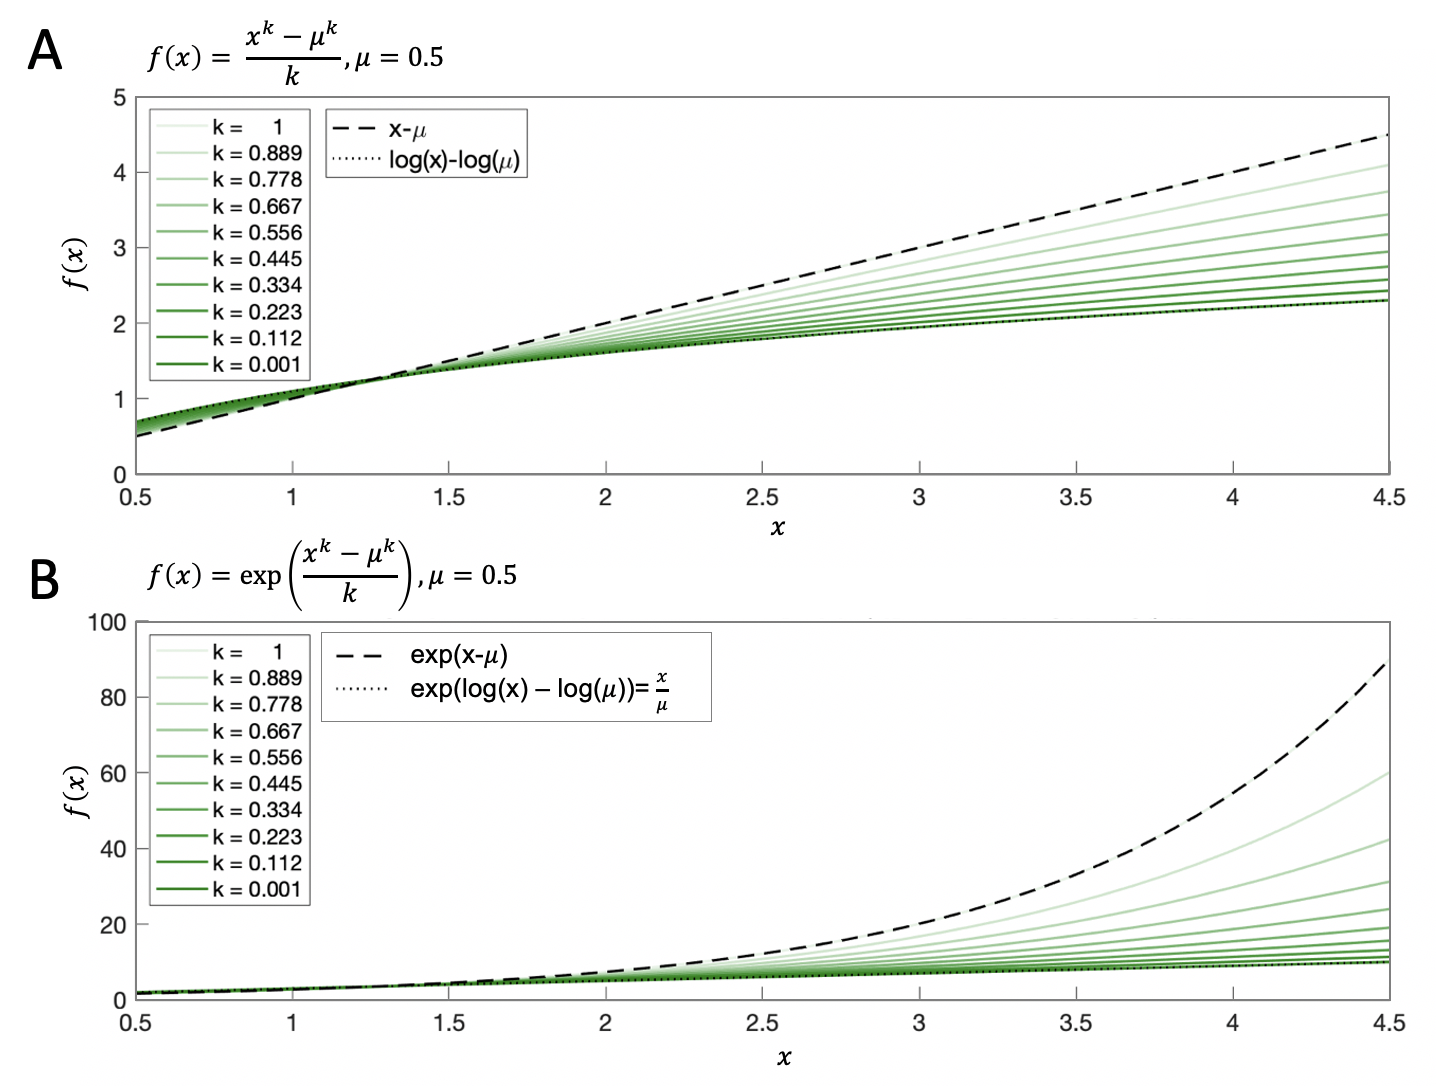
\includegraphics[width=1\linewidth]{figures/decoy-log} 

}

\caption[Model compression approximation]{Illustration of variations in parameter $k$. $\textbf{A:}$ Using parameter $k$ to interpolate between a linear expression and its logarithmic compression. Note that the darkest green curve ($k=0.001$) lies on the dotted line (logarithmic expression), suggesting that implementing a value of $k$ as high as 0.001 satisfactorily approximates the natural logarithm. $\textbf{B:}$ Exponentiating the function from panel A,  as in the logistic formulation of the grandmother model. Note that the darkest green curve ($k=0.001$) lies on the dotted line (linear expression, $\exp(\log(x)-\log(\mu))=\frac{x}{\mu}$). This demonstrates that we can recover both normalization models that rely on logistic compression and normalization models that do not.}\label{fig:decoy-log}
\end{figure}

\hypertarget{grandmother-model-derivations}{%
\subsubsection{Grandmother Model Derivations}\label{grandmother-model-derivations}}

The adaptive gain, vanilla and recurrent divisive normalization, and range normalization models were nested within the grandmother model. This section shows how each of them can be derived from the general grandmother model equation.

Leveraging the limit from Eq. \eqref{eq:decoy-limit}, when we plug in the parameter values for vanilla divisive normalization specified in Table \ref{tab:decoy-table-grandmother} into the general grandmother model, we arrive at the formulation of vanilla divisive normalization (as per Eq. \eqref{eq:decoy-vdn}):

\begin{table}

\caption{\label{tab:decoy-table-grandmother}Parametrizations of grandmother model corresponding to computational schemes proposed in the literature.}
\centering
\begin{tabular}[t]{lllrrll}
\toprule
Model & $c_i$ & $s$ & $\beta_1$ & $\beta_2$ & $k$ & $\tau$\\
\midrule
VDN & $free$ & 1 & 0 & 1 & 0.001 & $free$\\
RDN & $free$ & 1 & 1 & 1 & $0.001$ & $free$\\
AG & $free$ & $free$ & 1 & 1 & $1$ & $free$\\
RN & 0 & 1 & 0 & 0 & 0.001 & $free$\\
\bottomrule
\end{tabular}
\end{table}

\begin{equation}
u_i(A_i) = \frac{1}{e^{-(v(A_i)^{0.001}-\mu_i^{0.001})(0.001)^{-1}}} = \frac{1}{e^{-(\log{v(A_i)}-\log{\mu_i})}} = \frac{1}{\frac{\mu_i}{v(A_i)}} = {\frac{v(A_i)}{\mu_i}} = {\frac{v(A_i)}{v(avg^{ABD}_i)+c_i}}
\end{equation}

Similarly, we may simplify the grandmother model into recurrent divisive normalization (Eq. \eqref{eq:decoy-rdn}) by plugging in the relevant parameter values specified in Table \ref{tab:decoy-table-grandmother}:

\begin{equation}
\begin{aligned}
u_i(A_i) = \frac{1}{1+e^{-(v(A_i)^{0.001}-\mu_i^{0.001})(0.001)^{-1}}} = \frac{1}{1+e^{-(\log{v(A_i)}-\log{\mu_i})}} = \\
\frac{1}{1+\frac{\mu_i}{v(A_i)}} = {\frac{v(A_i)}{v(A_i)+\mu_i}} = {\frac{v(A_i)}{v(A_i)+v(avg^{ABD}_i)+c_i}}
\end{aligned}
\end{equation}

Note that if we allow parameter \(s\) to vary freely, it assumes the role of a power transform for inputs:

\begin{equation}
\begin{aligned}
u_i(A_i) = \frac{1}{1+e^{-(v(A_i)^{0.001}-\mu_i^{0.001})(s \cdot 0.001)^{-1}}} = \frac{1}{1+e^{-(\log{v(A_i)}-\log{\mu_i})^{s^{-1}}}} = \\ \frac{1}{1+\frac{\mu_i^{s^{-1}}}{v(A_i)^{s^{-1}}}} =  {\frac{v(A_i)^{s^{-1}}}{v(A_i)^{s^{-1}}+\mu_i^{s^{-1}}}} = {\frac{v(A_i)^{s^{-1}}}{v(A_i)^{s^{-1}}+(v(avg^{ABD}_i)+c_i)^{s^{-1}}}}
\label{eq:decoy-power-eq}
\end{aligned}
\end{equation}

Similarly, we may obtain the formulation of range normalization (Eq. \eqref{eq:decoy-rn}) by plugging in the relevant parameter values from Table \ref{tab:decoy-table-grandmother} into the general grandmother model:

\begin{equation}
u_i(A_i) = \frac{1}{e^{-(v(A_i)^{0.001}-\mu^{0.001}_i)(0.001)^{-1}}} = \frac{1}{e^{-(\log{v(A_i)}-\log{\mu_i})}} = \frac{1}{\frac{\mu_i}{v(A_i)}} = {\frac{v(A_i)}{\mu_i}} = {\frac{v(A_i)}{v(rng^{ABD}_i)}}
\end{equation}

Finally, we may reduce the grandmother model to adaptive gain (Eq. \eqref{eq:decoy-ag}) by plugging in the relevant parameter values from Table \ref{tab:decoy-table-grandmother}:

\begin{equation}
\begin{aligned}
u_i(A_i) = \frac{1}{1+e^{-(v(A_i)-\mu_i) \cdot s^{-1}}} = \frac{1}{1+e^{-({v(A_i)}-{\mu_i}) \cdot s^{-1}}} = \frac{1}{1+e^{-({v(A_i)}-v(avg^{ABD}_i)-c_i)\cdot s^{-1}}}
\end{aligned}
\end{equation}

\begin{figure}

{\centering 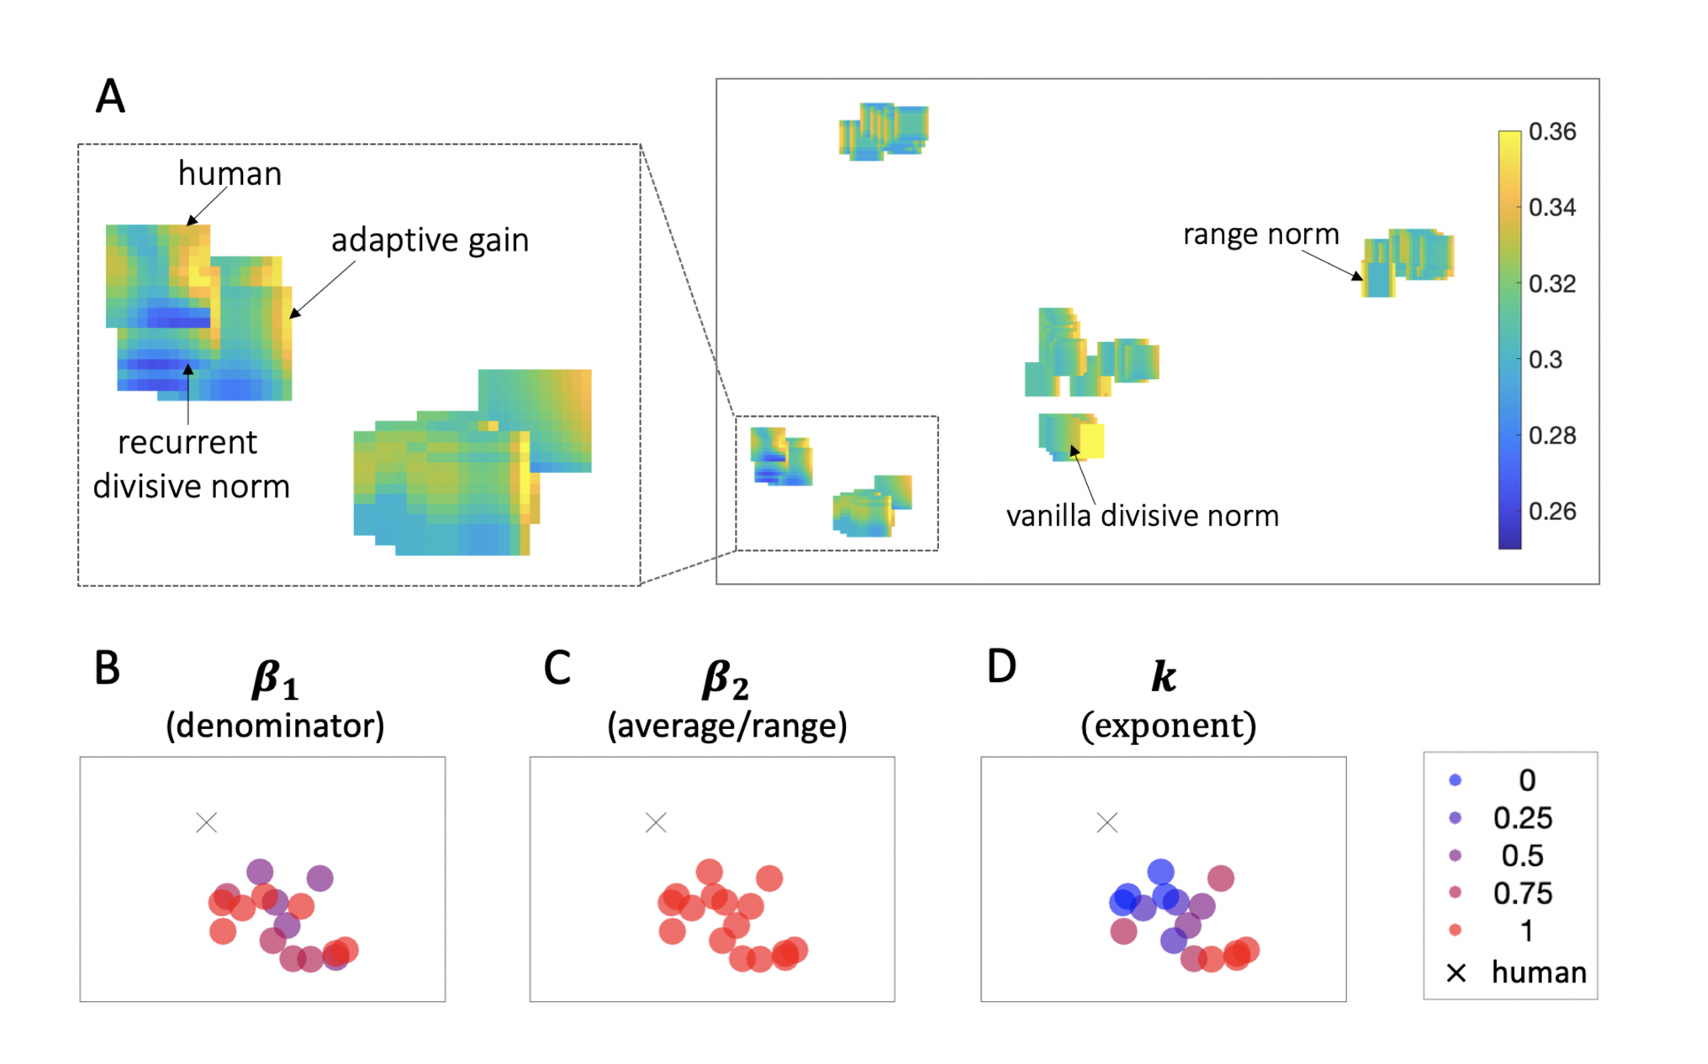
\includegraphics[width=1\linewidth]{figures/decoy-grandmother} 

}

\caption[T-SNE plot of model maps]{Charting decoy models. $\textbf{A:}$ Embedding space for normalization models of decoy effects. A $t$-distributed stochastic neighbour visualization of the maps of decoy influence produced by different variants of the grandmother model. Each map represents a variant of the grandmother model positioned in 2D space such that models with similar decoy influence patterns are nearby, while models with more different decoy patterns are further apart. Heat maps illustrate decoy influence. The rectangle on the left shows a zoomed in version of the denoted subset of embedding space. $\textbf{B-D:}$ These plots depict the zoomed in subset of embedding space presented above. Each model-produced decoy map is denoted as a dot and color coded to indicate parameter value: $\beta_1$ (panel B), $\beta_2$ (panel C), or $k$ (panel D). Human data is represented with a cross.}\label{fig:decoy-grandmother}
\end{figure}

Note that along with those specific models, which have been described in the literature, there exist many more parametrizations of the grandmother model which correspond to ``hybrid'' normalization schemes, combining specific features of the above described accounts.

\hypertarget{fitting-the-grandmother-model}{%
\subsubsection{Fitting the Grandmother Model}\label{fitting-the-grandmother-model}}

\hypertarget{methods-2}{%
\paragraph{Methods}\label{methods-2}}

We fit 125 variations of the grandmother model, by varying \(\beta_1\) and \(\beta_2\) in 5 steps between 0 and 1, and \(k\) in 5 steps between 0.001 and 1, in addition to the four constrained parametrizations of the grandmother model that result in the vanilla divisive normalization, recurrent divisive normalization, adaptive gain and range normalization models (Table \ref{tab:decoy-table-grandmother}). We used the \(t\)-distributed stochastic neighbor embedding (t-SNE) visualization technique \autocite{vandermaaten2008} to calculate relations among the resulting decoy influence maps from the 129 parametrizations. We specified the t-SNE hyperparameter perplexity, which controls the number of expected close neighbors, following guidelines in the literature to balance the trade-off between perplexity and the Kullback--Leibler divergence \autocite{cao2017}.

\hypertarget{results-2}{%
\paragraph{Results}\label{results-2}}

Fitting the grandmother model to human data revealed the different patterns of decoy influence predicted by variations of the general coding scheme. The embedding plot in Fig. \ref{fig:decoy-grandmother}a shows the simulated decoy maps for each of the 129 parametrizations of the grandmother model. Neighboring maps reflect models that produce relatively similar patterns of decoy influence (and vice versa for distant points). In Fig. \ref{fig:decoy-grandmother}b-d the points are colored according to levels of \(\beta_1\), \(\beta_1\) and \(k\), revealing the human data is neighbored by maps generated by models with high values of parameters \(\beta_1\) and \(\beta_2\), i.e.~those that resemble the adaptive gain model.

We note that the precise value of parameter \(k\), which interpolates between models implementing logistic and linear divisive normalization, is less important for fitting human data. This implies that the model is equally well fit with an exponentiated implementation of recurrent divisive normalization (\(k = 1\), such as the adaptive gain model) and with a linear implementation of recurrent divisive normalization (\(k\) \textasciitilde{} \(0\)), where inputs are transformed with a power parameter \(s\) prior to normalization (\(s\neq 0\), see Eq. \eqref{eq:decoy-power-eq}). This latter formulation of recurrent divisive normalization (as in Eq. \eqref{eq:decoy-power-eq}) is conceptually analogous to a form of recurrent divisive normalization in which values are power transformed \autocite[as in][]{daviet2018}:
\begin{equation}
u_i(A_i)^{PRDN} = \frac{v(A_i)^{\alpha}}{v(A_i)^{\alpha}+v(avg_i^{ABD})^{\alpha}+c_i}
\label{eq:decoy-prdn}
\end{equation}

Indeed, Bayesian model selection reveals that this model fits the data equally well as the adaptive gain model (exceedance probability for PRDN = 0.49), suggesting that our dataset cannot arbitrate between an exponential and power transform of attribute values.

Why is the nonlinear compression of attribute values important? To explore the role of this procedure, we compared the maps of decoy influence produced by an implementation of the grandmother model incorporating a logistic (i.e.~exponential) transform of attribute values (equivalent to the adaptive gain model) and an implementation of the grandmother model incorporating attribute values linearly (equivalent to recurrent divisive normalization without a power transform) in Fig. \ref{fig:decoy-nonlinearity}a. The nonlinearity qualitatively changes the form of the decoy map. The model featuring linearly coded attribute values produces stronger contextual effects for decoys of higher attribute values. This result can be traced back to the shape of the transducer function under linear attribute values (Fig. \ref{fig:decoy-nonlinearity}b, red curve), which is a non-symmetric concave function. Consequently, the curve deviates more from the identity line along the higher end of the abscissa and this leads to higher distortions in the translation of higher compared lower attribute values.

\begin{figure}

{\centering 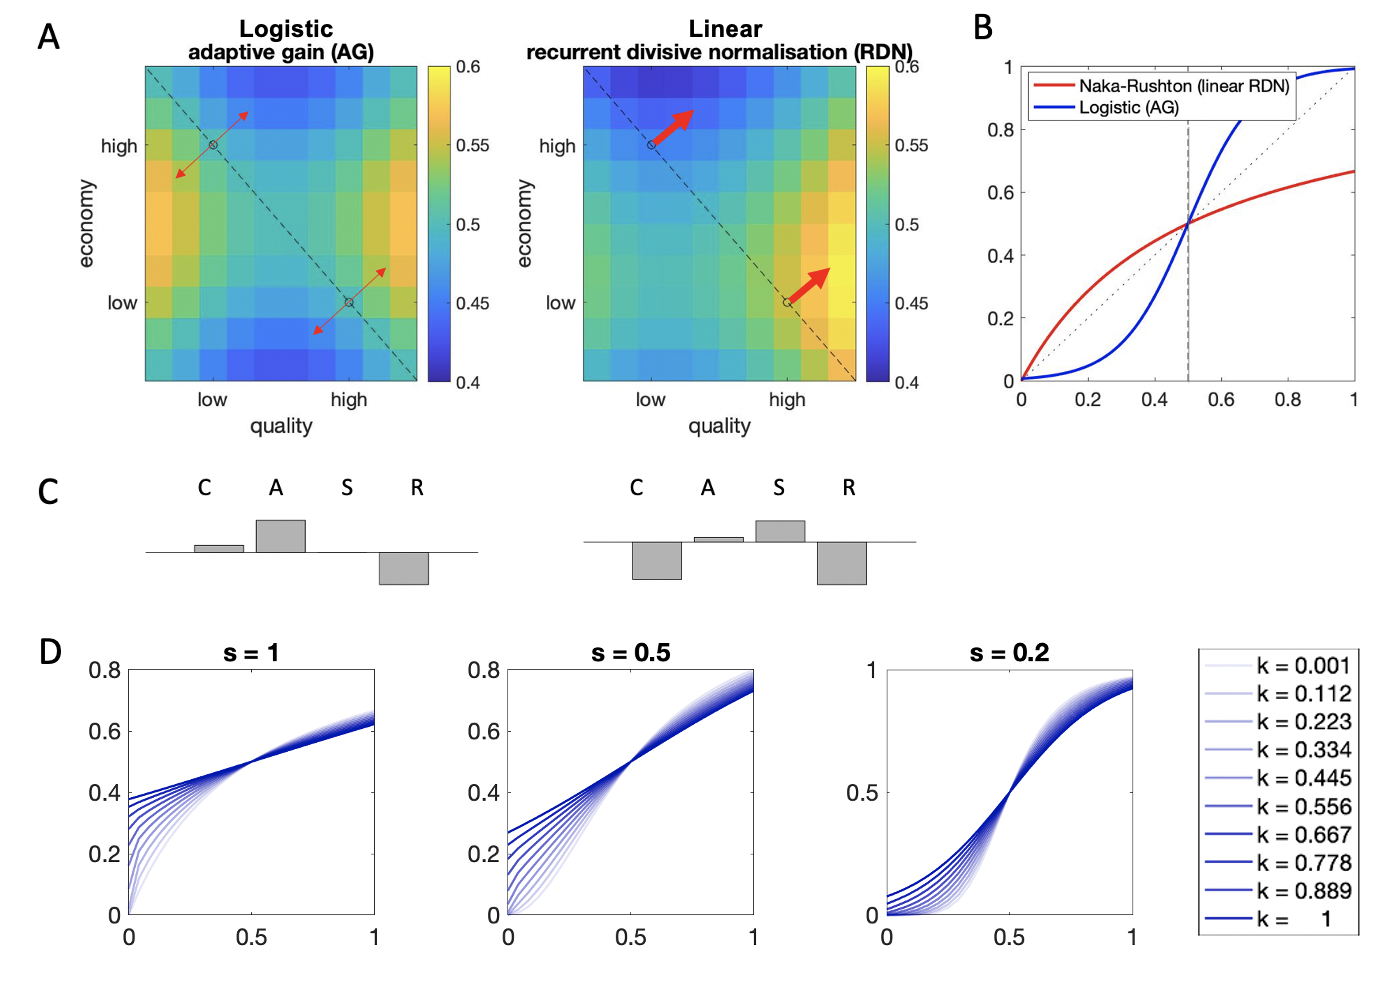
\includegraphics[width=1\linewidth]{figures/decoy-nonlinearity} 

}

\caption[Normalization with compressed inputs]{The role of the compressive nonlinearity. $\textbf{A:}$ Simulated decoy maps for the adaptive gain and recurrent divisive normalization models. It is noteworthy that the adaptive gain model (with bias terms $c_i=c_j=0$) produces symmetric regions of repulsion and attraction around the line of isopreference. By contrast, "linear" recurrent divisive normalization (i.e. RDN without a power transform applied to values prior to transduction) produces stronger repulsion and attraction for superior decoys (i.e. decoys above rather than below the isopreference line). $\textbf{B:}$ The asymmetric pattern of decoy influence seen for linear RDN occurs because the transducer is a (decelerating) Naka-Rushton function. This function is concave, meaning that the derivative is always higher (i.e. curve steeper) for low than high attribute values irrespective of the value of $x$. By contrast, the transducer for AG is sigmoidal and it is thus symmetric around the midpoint (which is itself adjusted to the context; this is the “adaptive” part). This panel plots the transductions applied to inputs by the Naka-Rushton function in red and by the Sigmoidal function in blue, with $v((avg)_i)=0.5$ (dashed line), $s=0.1$. The recurrent divisive normalization framework (without additional nonlinearity) implies that those attribute values which are always relatively smaller (closer to zero) are processed with higher gain. By contrast, the adaptive gain model implies that resources are allocated preferentially to the mean of a context, exaggerating binary distinctions which potentially straddle that midpoint (e.g. “low” vs. “high” value). $\textbf{C:}$ The relative strengths of the compromise, attraction, similarity and repulsion effects per the two decoy maps. $\textbf{D:}$ Illustration of the transfer function of the grandmother model, with $c_i=c_j=0$, $\beta_1=\beta_2=1$, and $v((avg)_i)=0.5$, across different values of $k$ and $s$. Note that with this parametrization, the transducer function is equivalent to a logistic function when $k=1$, and to a Naka-Rushton function when $k \sim 0$ and $s=1$. Power transforming inputs (by setting $s \neq 1$) in the Naka-Rushton definition approximates the sigmoidal shape of the adaptive gain transducer.}\label{fig:decoy-nonlinearity}
\end{figure}

This is in contrast to what happens in the presence of an exponential nonlinearity as in the adaptive gain model. This compression of attribute values produces an S-shaped transducer (Fig. \ref{fig:decoy-nonlinearity}b, blue curve), akin to the sigmoidal shapes of response functions ubiquitous in neural coding. Notably, this transducer is symmetric around the inflection point (which corresponds to the mean of attribute values of the context when \(c_i=0\)) and thus results in equal levels of distortion across the low and high end of attribute space. The bias term \(c_i\) can tip the balance in either direction: it can produce stronger effects for higher attribute values when \(c_i>0\) and stronger effects for lower attribute values when \(c_i<0\) (see Fig. \ref{fig:decoy-sim}d for simulations). Of note, the sigmoidal shape of the transducer here can be approximated by power transforming inputs prior to normalizing them in the recurrent divisive normalization scheme (i.e.~\(s>0\) and \(k\sim 0\), Fig. \ref{fig:decoy-nonlinearity}d lightest blue curve). This result helps clarify why this operation can capture the human data equally well as the exponential nonlinearity in the adaptive gain model.

Finally, we asked whether the adaptive gain model fits better than the full grandmother model after appropriate penalization for complexity. A failure to do so would imply the existence of a ``hybrid'' normalization solution that fits the human data even better, presumably involving some combination of parameters that has yet to be described in the literature. To asses this, we performed Bayesian model selection on complexity-penalized model fit metrics (Bayesian Information Criterion, BIC) which revealed that the exceedance probability for the normalization scheme favored by our empirical data, the adaptive gain model, over the grandmother model is 0.97, offering evidence against a hybrid solution.

\hypertarget{interim-discussion-1}{%
\subsection{Interim Discussion}\label{interim-discussion-1}}

Altogether, the results of our modeling suggest that a very simple computational scheme appealing to the relative encoding of attribute values may capture the full pattern of decoy influence in our dataset. We identified a 5-parameter model, previously termed adaptive gain, which fit the data exceptionally well, both at a fine scale (at the level of effects in individual participants) and on the aggregate level (the average map of decoy influence). We compared this model to related theoretical accounts in the literature, which appeal to a contextual normalization of attribute values, first, via conventional model selection techniques and second, through a comprehensive model comparison exercise for which we devised a flexible ``grandmother'' model encompassing a wide space of putative normalization schemes. The results of our computational work indicated that the rich pattern of decoy influence is best accounted for by information processing schemes that compressively transduce inputs, appealing to normalization by the central tendency of context and recurrently overweighing the contribution of the target input to the normalization.

\hypertarget{discussion}{%
\section{Discussion}\label{discussion}}

Decoy effects have been studied for decades, but substantial controversy has surrounded their replicability, interrelationship, and computational origins. This chapter sheds new light on these debates by gathering and analyzing a large-scale dataset that systematically maps the influence of a decoy stimulus across both the inferior and superior locations of multiattribute space. Conducting our analysis in a conventional fashion, we broadly replicate past studies, in that we find strong attraction effects, strong compromise effects, and a weaker and more variable similarity effect (not significant in our dataset). As in previous studies, the three decoy effects are correlated across the cohort, with a positive relationship observed between attraction and compromise, and a negative relationship between those two and the strength of the similarity effect \autocite{berkowitsch2014}. This finding implies that three decoy phenomena have a single cause, and indeed previous dynamic models (in which information is accumulated over time) have been able to capture the three discrete effects with a single set of parameters \autocite{roe2001,usher2004,bhatia2013,trueblood2014,bhui2018}. Here, we use dimensionality reduction on the full decoy influence map to confirm that indeed, there is a single component that explains the vast majority (\textasciitilde95\%) of the variance in decoy influence, suggestive of a single computational origin for these biases.

To understand the computational origin of decoy effects, we chose to model our data with a framework based on divisive normalization. We made this choice because the normalization model offers a simple, parsimonious account of contextual biases in decision-making based on a rich, neurobiologically grounded tradition in the cognitive sciences \autocite{carandini2012,louie2013,rigoli2019,landry2021,webb2021}. In particular, it allowed us to systematically measure the influence of various candidate computational steps on the predicted decoy map, providing an interpretable mapping from model to data (Fig. \ref{fig:decoy-sim}). On this basis, we were able to establish (for example) that normalization occurs relative to the average of the available values (via a sigmoidal gain function) rather than to the lower end (via a concave gain function) as proposed in some previous models (Fig. \ref{fig:decoy-nonlinearity}). This characteristic sigmoidal shape of the transfer function may be approximated by transforming inputs via a power term (\(\alpha>1\)) in recurrent divisive normalization \autocite{daviet2018,webb2021}.

Overall, out of the models tested here, evidence favored a model that has previously been described in the literature as the \emph{adaptive gain model} \autocite{cheadle2014,li2018}. This account is closely related to other models involving recurrent divisive normalization, especially those proposing that values are nonlinearly transformed beforehand, as well as being very similar to another model known as the logistic model of subjective value \autocite{rigoli2019}. There is a close correspondence between qualitative features of model-simulated and human performance displayed in Fig. \ref{fig:decoy-map}, and in particular, a close correspondence achieved after decomposition of the decoy map into linear components using singular value decomposition (Fig. \ref{fig:decoy-svd}). The adaptive gain model even predicted a new and potentially counter-intuitive relationship between the decoy effects: that when the compromise effect is positive, attraction should dominate over repulsion (and vice versa), a prediction that was satisfied in the data.

Under the adaptive gain control framework described here, decoy effects occur because of contextual biases arising when each target item is transduced via a logistic function whose inflection point lies at the mean of all three items including the decoy. For example, the ``attraction'' effect thus occurs because when the decoy is lower in value than item A, the inflection point is lower than item A, and so A lies at the steepest portion of the sigmoidal gain function and is thus ``overvalued'' or repulsed away from this mean point. The precise converse occurs when the decoy is higher in value than A, as well as for B. Previous work has demonstrated that exactly this mechanism can in principle account for a range of decision biases arising in the presence of distractors, across perceptual, cognitive and economic domains \autocite{li2018}. The brain may have evolved the type of normalization scheme proposed here because it promotes efficient neural coding \autocite{summerfield2015,summerfield2020}.

Whereas the attraction effect tends to be highly robust and consistent across participants, the strength and directionality of the compromise effect and similarity effects tend to be more idiosyncratic. Indeed, the similarity effect did not reach statistical significance in our dataset. In our model, the compromise and similarity effects occur when attractive and repulsive processes are asymmetric due to differential weighing or biasing of the two attributes, causing attraction effects (and their converse for superior decoys) to warp and/or ``spill over'' into locations where compromise and similarity decoys are typically tested. In other words, the fragile nature of the compromise and similarity effects might be at least in part due to heterogeneity in the asymmetric way each attribute is coded or transformed, which in turn might (for example) be due to differing choice concerning stimulus materials. A systematic unpicking of ways in which different classes of stimulus material (e.g.~numerical values in distinct ranges, perceptual stimuli such as rectangles, and vignettes) are encoded, and thus why decoy effects may or may not have emerged in previous studies \autocite{frederick2014,huber2014,spektor2021}, is beyond the scope of our research project here. However, our simulations suggest that a relatively low-dimensional encoding model may be sufficient to capture this variation and thus to pinpoint the source of variation in previous studies.

\hypertarget{conclusion}{%
\section{Conclusion}\label{conclusion}}

Adding a ``decoy'' alternative to a choice set can shift preferences in multialternative economic decisions. A long research tradition focusing on this contextual bias has provided evidence for three classic decoy effects -- the compromise, attraction and similarity effects -- but their replicability, interrelationship and computational origins have sparked controversy. To address these, we carried out a large-scale incentive-compatible study, charting the full two dimensional attribute space of decoy effects. Our analyses indicated that a single explanatory factor can account for the rich pattern of decoy influence we observe. Indeed, a simple process model, appealing to the principle of divisive normalization, can capture our results both at the individual and aggregate level.

\hypertarget{acknowledgements}{%
\section{Acknowledgements}\label{acknowledgements}}

This chapter is based on the published work \emph{Dumbalska, T., Li, V., Tsetsos, K., \& Summerfield, C. (2020). A map of decoy influence in human multialternative choice. Proceedings of the National Academy of Sciences, 117(40), 25169-25178.}

The human data for this chapter was procured by Dr Vickie Li. Dr Vickie Li and Prof Christopher Summerfield jointly designed and Dr Vickie Li built the experiment and administered data collection. Dr Konstantinos Tsetsos provided feedback on code for the modeling simulations.

\begin{savequote}
\emph{This chapter is based on a manuscript under peer review:}

Dumbalska, T., Rudzka, K., Smithson, H. E., \& Summerfield, C. (2021).
How do (perceptual) distractors distract?
\qauthor{}\end{savequote}

\hypertarget{distr}{%
\chapter{How do perceptual distractors distract?}\label{distr}}

\minitoc

\noindent 
\emph{When a target stimulus occurs in the presence of distractors, decisions are less accurate. But how exactly do distractors affect choices? This chapter explores that question using measurement of human behavior, psychophysical reverse correlation and computational modeling. We contrasted two models: one in which targets and distractors have an independent influence on choices (independent model) and one in which distractors modulate choices in a way that depends on their similarity to the target (interaction model). Across three experiments, participants were asked to make fine orientation judgments about the tilt of a target grating presented adjacent to an irrelevant distractor. We found strong evidence for the interaction model, in that decisions were more sensitive when target and distractor were consistent relative to when they were inconsistent. This consistency bias occurred in the frame of reference of the decision, that is, it operated on decision values rather than on sensory signals. Further, it was independent of spatial attention. A normalization framework, where target features are normalized by the expectation and variability of the spatial context, successfully captures the observed pattern of results.}

\hypertarget{introduction-2}{%
\section{Introduction}\label{introduction-2}}

Visual scenes in the real world are typically cluttered, and so perceptual decisions necessarily occur in the context of irrelevant information. For instance, when adjusting a crooked picture frame, a decision maker must focus on its offset from vertical, ignoring the tilts of surrounding paintings, as those are irrelevant to the task. A long line of research across psychology and neuroscience has investigated humans' ability to focus on an imperative stimulus in the context of distracting input. A classic laboratory analogy of the above scenario asks participants to judge a cued item in a multi-element array. For example, participants might be asked to discriminate the tilt of a (cued) target grating presented among one or more irrelevant gratings (distractors). Empirical work has focused on understanding how the cue impacts behavior and modulates neural signals, informing models of how target processing is prioritized in the face of distraction \autocite{reynolds2004,carrasco2011}. These models have, for example, produced detailed predictions about how tuning functions in visual neurons vary according to whether the neuron's preferred stimulus is attended or unattended \autocite{moran1985,mcadams1999,treue1999,reynolds2009}.

However, we know remarkably little about how distraction itself influences decisions. When (a cued) target and (an uncued) distractor occur together, how exactly does the distractor affect choices? This question lies at the intersection of several distinct literatures in psychology and neuroscience which are rarely discussed together. Firstly, it is sometimes argued the effects of spatial cueing can be understood through the normative lens provided by Bayesian inference. The cue provides probabilistic information about which of two locations is decision-relevant; an ideal observer will combine this with noisy signals arising from target and distractor locations, weighted by their likelihoods \autocites[according to the probabilistic cue,][]{dayan1999,eckstein2009}. In other words, the distractor and target hold independent sway over decisions, with the job of the observer being to weigh them appropriately according to prior information. Similar models have sometimes tried to subsume the literature on attention within the normative framework given by decision theory \autocite{anderson2011}.

A related view of distraction can also be found in a popular theoretical framework proposing that stimuli effectively compete for neural resources. Attention serves as controller that can bias processing towards percepts which are more relevant for ongoing behaviors \autocite{desimone1995}. While this view does not clearly translate onto decision theory, it nevertheless implies that decision variables are derived from admixtures of independent (relevant and irrelevant) sensory signals, with their relative weighing determined by the strength of control, for example arising in prefrontal cortex \autocite{miller2001,egner2005}. Alternative but related views posit that relevant and irrelevant features race independently to drive decisions \autocite{bundesen1990} or contribute to the differential weighing of mutually inhibitory sources of evidence in an accumulation-to-bound model, a framework known as decision field theory \autocite{busemeyer1993}. One specific instance of this class of theory argues that when humans choose between a preferred and a less preferred item, inputs to the decision process are given by a subtractive mixture of the two stimulus values, with a higher weight given to the currently fixated item \autocite{krajbich2010}.

What the aforementioned models share is the central idea that target and distractor contribute independently to choice. Broadly, we can view decisions as driven by a process such as:
\begin{equation}
y^{ind} = \beta_0 + \beta_1\theta_T + \beta_2\theta_D + \epsilon
\end{equation}
where \(y^{ind}\) is the decision variable, \(\theta_T\) and \(\theta_D\) are the features of the target and distractor respectively, \(\beta_1\) and \(\beta_2\) are their respective weights, and \(\epsilon\) is an error term. We can consider the application of the weights to be outside voluntary control, so that distraction is at least in part inevitable. Here, we call this the ``independent'' model of distraction. For the most part, assuming that accuracy is above chance, we can expect \(\beta_1>\beta_2\). Some theories posit special downstream mechanisms that attempt to eliminate the effect of \(\beta_2\) altogether, known as distractor suppression \autocite{geng2014,chelazzi2019}.

However, a different proposal is that target and distractor do not wield independent sway over \(y\) but rather:
\begin{equation}
y^{int} = \beta_0 + \beta_1\theta_T + \beta_2\cdot f(\theta_T|\theta_D) + \epsilon
\end{equation}
We use the term \(f(\theta_T|\theta_D)\) in this equation to refer to some unspecified process by which target and distractor interact. For instance, this could be a straightforward multiplicative process or it could involve rectification or discretization operations; e.g.~target processing could be stronger or weaker when the distractor is similar/dissimilar \autocite{blakemore1970} or congruent/incongruent \autocite{eriksen1974}. Importantly, what this implies is that the influence of the distractor on the decision occurs only by virtue of how the distractor modulates or interacts with the target. Thus, we call this the ``interaction'' model of distraction.

This class of model has also been popular at various times and in various guises. For instance, one well-known body of literature discusses the phenomenon of contextual facilitation, whereby in the extrastriate visual cortex, neuronal responses to the receptive field center are biased by stimulation of the surround \autocite{krause2014}. At the neural level, this area has been amply explored but fewer studies have examined how spatial context may modulate behavior. Still, previous work has established that detection thresholds for a grating are lowered if it is flanked by collinear gratings \autocite{polat1994,kapadia1995,ito1999,gilbert2013}. Here, the distractors influence the decision by virtue of their similarity to the target. Another example involving visual stimuli is the tilt illusion whereby the tilt of a central grating is perceived as repulsed away from a ring of flanking distractors \autocite{blakemore1970}. Again, the distractors do not influence the decision directly; for instance, decisions about the target are less repulsed if the distractors are more dissimilar, contrary to the predictions of the independent model. These sensory level interaction effects have been successfully modeled in a divisive normalization framework, where individual neural responses are scaled by the population response \autocite{carandini2012}.

Indeed, the family of normalization models discussed in the previous chapter, which successfully capture decoy effects in decisions about economic prospects, also constitute specific instances of the interactive model. In this class of models, known as divisive normalization, \(f(\theta_T|\theta_D)\) may be viewed as a divisive operation, following the general form \(y \sim \frac{\theta_T}{r+\theta_T+\theta_D}\), where \(r\) is a regularizer \autocite{louie2013,landry2021}. Through the years, alternative explanations of the phenomenon have sometimes instead appealed to the independent account \autocite{busemeyer1993}. However, it is difficult to reconcile those theories with findings that the modulation strength of a decoy depends on its proximity in conceptual space to the target \autocite{soltani2012,landry2021}, echoing results from the perceptual literature about the effect of target-distractor similarity on choice.

Relatedly, in the cognitive domain, perception of quantities (e.g.~the number of African nations) or value (the price of bottle of wine) can be anchored by irrelevant prior information \autocite{ariely2003}. However, anchoring by an irrelevant quantity also seems to diminish with distance between the anchor and the target value \autocite{wegener2001}, indicative of an interaction between target and distractors. Together, these effects from diverse literatures imply a view whereby distractors and targets interact. Indeed, a recent paper showed how a version of the interaction model can explain a range of distractor-mediated phenomena in perceptual, cognitive, and value-based decision tasks \autocite{li2018}.

This chapter describes three experiments in which participants made a fine discrimination judgement about a target grating that is presented concurrently with an irrelevant distractor grating. We combined computational modeling and reverse correlation analysis to probe how the distractor influences choices. This approach allowed us to directly compare variants of the independent and interaction models as explanations of our data. Our experiments addressed three related questions. Firstly, how does the distractor influence decisions? Secondly, does it do so at the perceptual or decision level? And thirdly, how does spatial attention mitigate (or otherwise) the effect of distraction?

\hypertarget{experiment-1}{%
\section{Experiment 1}\label{experiment-1}}

To investigate the influence distractors wielded on choice, we presented participants with brief flashes of a pair of Gabor patches embedded in smoothed noise. We analyzed participants' reports of the tilt of the target grating on each trial, using information about the features of the orientation signal of both target and distractor stimuli, as well as information about the signal-like fluctuations in the noise of each stimulus.

\hypertarget{methods-3}{%
\subsection{Methods}\label{methods-3}}

\hypertarget{participants-1}{%
\subsubsection{Participants}\label{participants-1}}

Twenty-six participants (aged 25.33 ±4.38) took part in Experiment 1. Two participants were excluded from the main analyses as the accuracy of their responses for one of the possible stimulus locations was at chance level (\textbar accuracy - 50\%\textbar\textless5\%). Our exclusion strategy took into account that 75\% accuracy (the staircase target and approximately the average performance in the experiment) could be achieved if participants only focused on one side of the screen (and achieved near 100\% accuracy for stimuli there) while guessing on the other side (achieving near 50\% accuracy for stimuli there). To ensure that such a strategy was not driving the observed level of accuracy, we excluded participants who performed at chance level for stimuli on either side of the screen. The study received ethical approval from the Central University Research Ethics Committee at the University of Oxford (approval reference number: R51752/RE001). All participants provided written informed consent and were compensated £10 per hour for their time.

\hypertarget{apparatus}{%
\subsubsection{Apparatus}\label{apparatus}}

Participants were seated in a dark room approximately 60cm away from a computer monitor (120Hz refresh rate, 1280x1024 resolution, 21' CRT) with linearized output light intensities. Visual stimuli were created and presented with Psychophysics Toolbox Version 3 \autocite[PsychToolbox-3,][]{brainard1997} for MATLAB.

\hypertarget{stimuli}{%
\subsubsection{Stimuli}\label{stimuli}}

The experimental stimuli were noisy gratings, each of which consisted of a Gabor pattern and smoothed Gaussian noise. The Gaussian envelope of the Gabor patterns had a standard deviation of 1° of visual angle. The phase of each Gabor pattern was sampled from a uniform distribution; orientation was drawn from a uniform distribution with range --10° to 10° rotation from a vertical decision boundary. Noise was generated independently for each stimulus by sampling pixel values from a Gaussian distribution and passing the resulting pixel values through a smoothing Gaussian filter. The dimension of the filter, 0.083° of visual angle, was chosen to maximize the trial-to-trial variability of the convolution between the smoothed noise and Gabor signal \autocite{wyart2012}. Stimuli were presented at full contrast. The ratio of the contrast of the Gabor pattern to the contrast of the noise of a stimulus was adaptively determined for each participant (see procedure for staircase details). The average value of the contrast ratio produced by the staircase across participants was 0.35 (i.e.~35\% of the contrast of the stimulus was dedicated to the signal and 65\% to the smoothed noise). Stimulus size spanned 4° visual angle and stimulus position was centered at 4° of visual angle to the left and right of fixation.

\hypertarget{experimental-procedure}{%
\subsubsection{Experimental Procedure}\label{experimental-procedure}}

Each participant completed the experiment in a single hour-long session. The experimental session consisted of 2 training blocks and up to 9 test blocks (100 trials each). The training blocks served to familiarize participants with the task and calibrate participant performance. To this end, during training we employed an adaptive staircase procedure, accelerated stochastic approximation \autocite{lu2013}, to titrate the contrast ratio for the noise in the stimuli for a target participant performance of 75\% correct. The training and test trials followed the same structure; the only difference was in the contrast ratio of the stimuli. During training blocks, the contrast ratio was adjusted in each trial according to the staircase, which varied the step size of the change in contrast adaptively after each response. The training blocks had a variable trial count. Each training block ended after the staircase converged and took on average between 5-10 minutes. We used the contrast ratio estimate from the second training block to generate stimuli for the test blocks.

\begin{figure}

{\centering 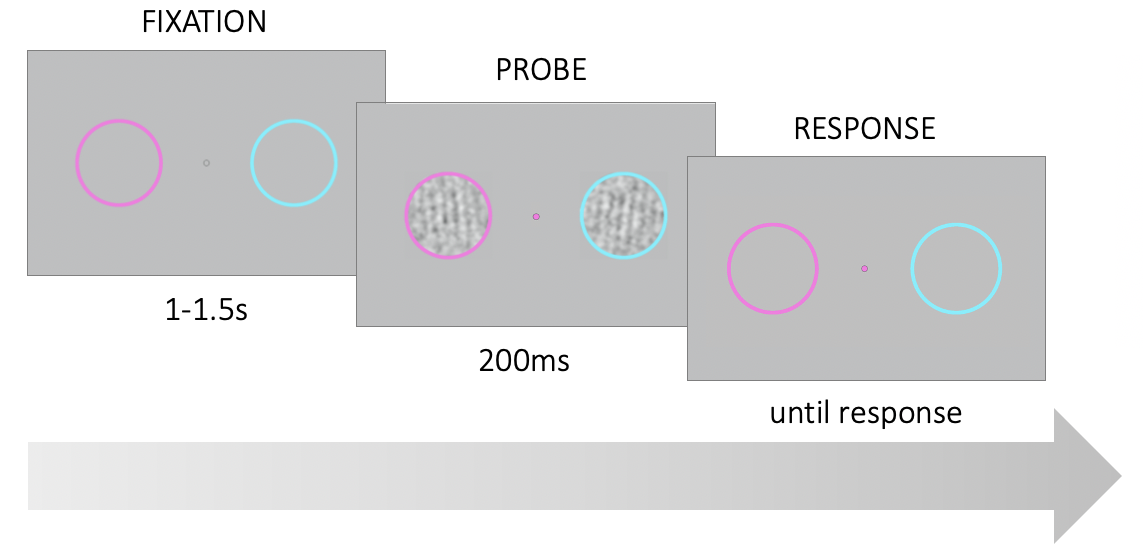
\includegraphics[width=1\linewidth]{figures/distr-trial-a} 

}

\caption[Experiment 1, Trial structure]{Trial structure. Participants were asked to fixate on a point in the center of the screen. Two noisy gratings appeared briefly within the colored rings on the left and right of the fixation point. At stimulus onset, the fixation point changed color and served as a probe. Participants had to report the tilt (CW or CCW) of the probed grating relative to vertical.}\label{fig:distr-trial-a}
\end{figure}

Each test block lasted approximately 5 minutes and participants were invited to take short breaks between blocks. During the experiment, participants were asked to fixate their gaze at the center of the screen on a fixation point between two colored rings (Fig. \ref{fig:distr-trial-a}). The rings were located at 4° of visual angle to the left and right of center. The left ring was magenta and the right ring was cyan. In each trial, after a uniformly variable interval between 1-1.5s, two noisy gratings appeared within the colored rings for 200ms. At stimulus onset, the fixation point assumed the color of one of the two rings until the end of the trial. The color of the fixation point served as the probe indicating which of the two stimuli was the target. Participants had to report whether the target was tilted clockwise or counterclockwise (CW or CCW) relative to a vertical decision boundary. Participants reported their responses via keyboard presses (left and right arrow keys) and instantaneously received fully informative auditory feedback (correct: a high 880Hz tone, incorrect: a low 440 Hz tone).

\hypertarget{analyses-1}{%
\subsubsection{Analyses}\label{analyses-1}}

In our analyses, we asked how the distractor stimulus affects participant choices. We addressed this question with both regression-based and reverse correlation analytic approaches.

\hypertarget{stepwise-regression}{%
\paragraph{Stepwise Regression}\label{stepwise-regression}}

We first took a regression-based approach to identify the contributions of the target and distractor to choice. We defined the decision-relevant features of the target \(\theta_T\) and distractor \(\theta_D\) as their respective angular offsets from the decision boundary on each trial. We assumed that choice probabilities were a logistic function of a decision variable \(y\), computed from both target and distractor features:
\begin{equation}
p(CW) = \frac{1}{1+e^{-y}}
\label{eq:distr-y}
\end{equation}
where \(p(CW)\) corresponds to the probability to respond clockwise on a given trial.

In order to ascertain the nature of the relationship between distractor features and choice, we utilized a forward and backwards stepwise regression approach for including predictors. Due to the way we have framed the question above, there is some liberty in specifying the nature of the target-distractor interaction. The hierarchical factor knock-in and knock-out approach of the stepwise regression allowed us to consider a number of possible definitions of the interactive relationship \(f(\theta_T|\theta_D)\) and empirically evaluate each of them. The predictor variables we considered included:

\begin{itemize}
\tightlist
\item
  \(\theta_T\), the independent effect of the target angular offset
\item
  \(\theta_D\), the independent effect of the distractor angular offset
\item
  \(|\theta_D|\), the absolute value of the distractor angular offset
\item
  \(congruency\), a binary indicator whether the angular offsets of the target and distractor fall on the same side of the category boundary
\item
  \(\theta_T \cdot \theta_D\), the (unsigned) multiplicative interaction between the target and distractor angular offsets
\item
  \(\theta_T \cdot |\theta_D|\), the multiplicative interaction between the target angular offset and the absolute value of the distractor angular offsets
\item
  \(\theta_T \cdot |\theta_T - \theta_D|\), the interaction between target angular offset and the consistency between the target and the distractor angular offsets
\end{itemize}

We estimated separate models for each individual participant. We used the \texttt{stepwise} algorithm from the MATLAB Statistics and Machine Learning Toolbox for the backward and forwards stepwise regression analysis and the Statistical Parametric Mapping Toolbox for Bayesian model selection. We used Bayesian model selection \autocite{stephan2009} to compare the cross-validated log likelihoods of the model identified with the stepwise regression against nested competitor models.

To further explore the effect of the distractor on choices, we used logistic regression to estimate target sensitivity across different values of the distractor. We sorted distractors into 6 bins, each bin spanning 3.33°, and regressed choices within each distractor bin on target offset, \(\theta_T\):
\begin{equation}
y = \beta_0 + \beta_1\theta_T
\end{equation}

Running this regression model separately for each distractor bin allowed us to estimate the influence of \(\theta_T\) given different values for \(\theta_D\) and detect distractor-dependent changes to target sensitivity.

\hypertarget{reverse-correlation}{%
\paragraph{Reverse Correlation}\label{reverse-correlation}}

The regression analysis describes each target and distractor with a scalar quantity that indexes the disparity between its orientation signal and the boundary. However, the target and distractor stimuli constituted images containing multidimensional information about a full range of orientations. In particular, the energy at each orientation varied from trial to trial for both target and distractor because of the smoothed noise we applied. This allowed us to carry out a reverse correlation analysis to examine how the signal-like fluctuations in signal energy at each orientation influence choices, and thus to plot decision kernels in orientation space for both target and distractor.

\hypertarget{stimulus-energy-profiles}{%
\subparagraph{Stimulus Energy Profiles}\label{stimulus-energy-profiles}}

\begin{figure}

{\centering 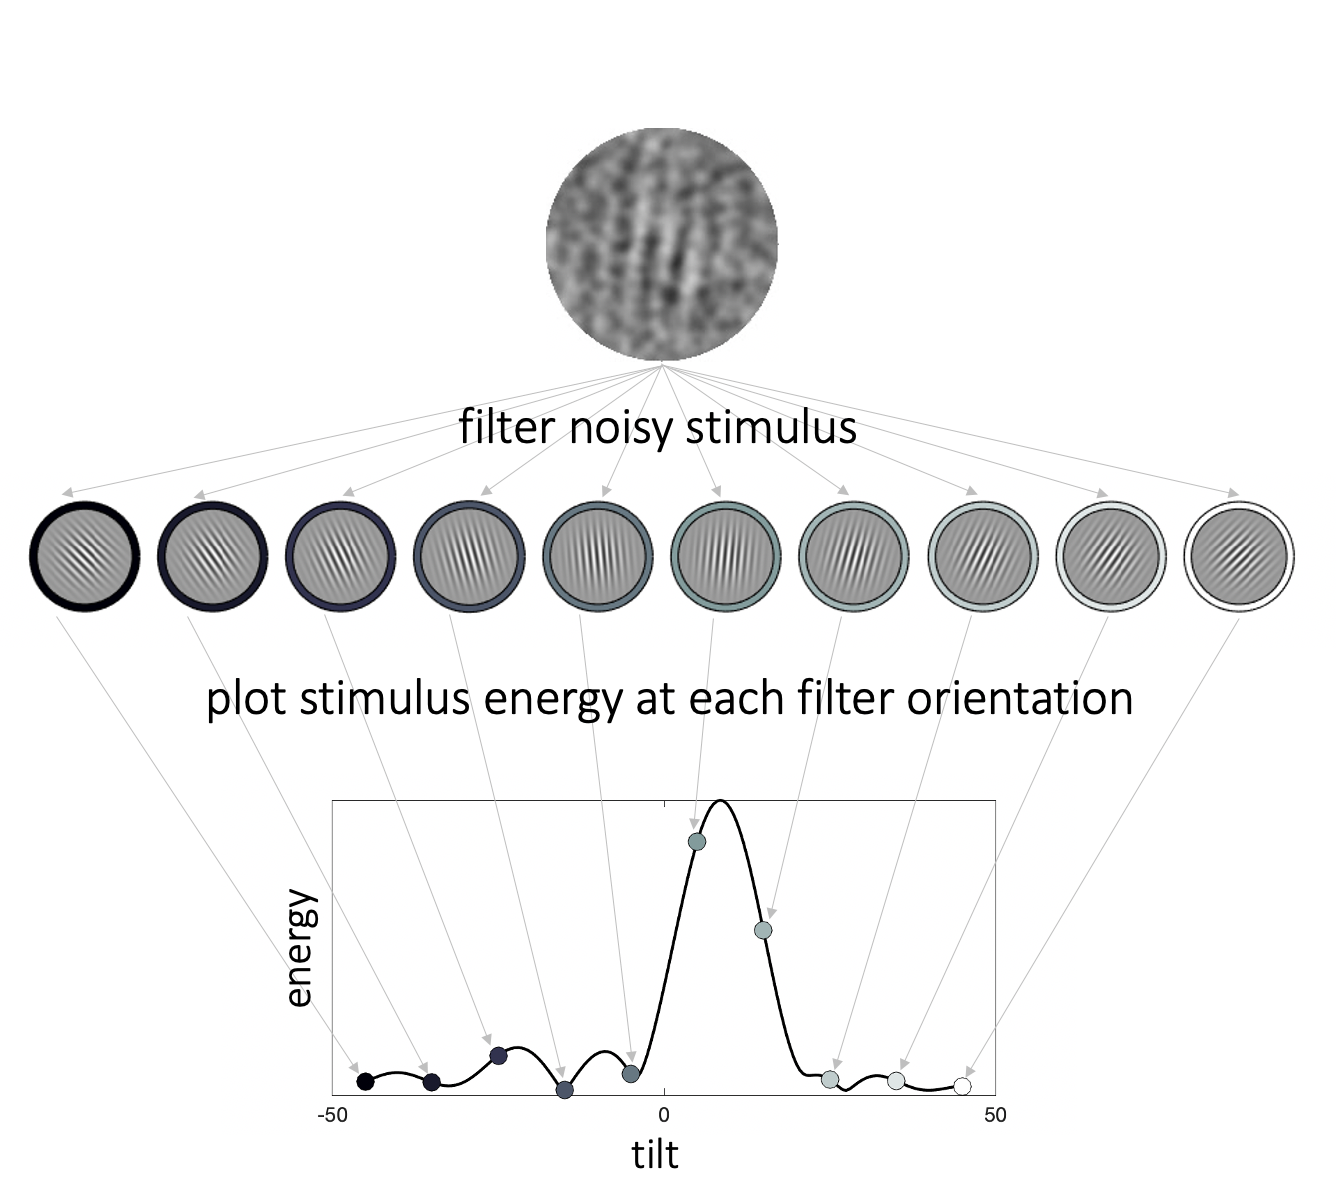
\includegraphics[width=0.75\linewidth]{figures/distr-methods-energy} 

}

\caption[Reverse correlation analysis, Stimulus energy]{Stimulus energy profiles. We filtered each noisy stimulus through a pool of oriented Gabor patches to calculate energy across orientation space. The higher the stimulus energy at a given orientation, the more the noisy stimulus resembles a Gabor patch of that orientation. The collection of energies of a given stimulus across orientation space constitutes the energy profile of that stimulus. }\label{fig:distr-methods-energy}
\end{figure}

To quantify the relationship between trial-to-trial signal-like fluctuations in the noise of each stimulus and participant decisions, we first characterized the filter energy of each stimulus \(S\) across orientation space using an ordered set of Gabor filters \(F^{\theta}_{\phi_n}\) (Fig. \ref{fig:distr-methods-energy}). The spatial frequency of the filters matched the spatial frequency of the Gabor patterns. Filter orientation (\({\theta}\)) ranged between -45° and 45° in increments of .5°. To correct for differences between the phase of the stimuli (sampled uniformly between \([0,1] \cdot 2\pi\)) and the filters, we specified 5 filter phases \({\phi_n}\) (\([0.1,0.9] \cdot 2\pi\), in steps of \(0.2 \cdot 2\pi\)). We calculated stimulus response to each filter \(R(S|F^{\theta}_{\phi_n})\) as the amount of variance in the filter that was explained by the covariance of the filter and stimulus. We then estimated the filter phase \(\phi^{max}\) (which can take any value between \([0,1] \cdot 2\pi\)) at which the highest response would be obtained for that orientation, by fitting the following mathematical model:
\begin{equation}
R(S|F_n^{\theta}) = E(S|\theta) \cdot \cos(\phi_n - \phi^{max})
\end{equation}
where \(E(S|\theta)\) corresponds to the energy of the stimulus \(S\) at orientation \(\theta\), and \(\phi_n\) to the phase of filter \(n\) (\(n\) ranges from 1 to 5). Thus, the model assumes that the relationship between filter response and filter phase follows a cosine function. We can use gradient descent to identify the value of \(\phi^{max}\) that would produce the strongest filter response, as well as predict the magnitude of that response, i.e.~signal energy at that orientation, \(E(S|\theta)\).

Calculating the energy profiles in this manner, that is, via convolution with Gabor filters of the same parametric specification as the target signal, ensures that we are obtaining orientation energy at the spatial scale of the target. This operation is more specific than, for instance, a Fourier transform in that it takes into account the expectation for the target (and distractor) signals. Thus, the energy profile lends itself to an intuitive interpretation -- the more a noisy stimulus resembles a signal grating with a given orientation, the higher the filter energy of the stimulus at that orientation.

\hypertarget{decision-kernels}{%
\subparagraph{Decision Kernels}\label{decision-kernels}}

\begin{figure}

{\centering 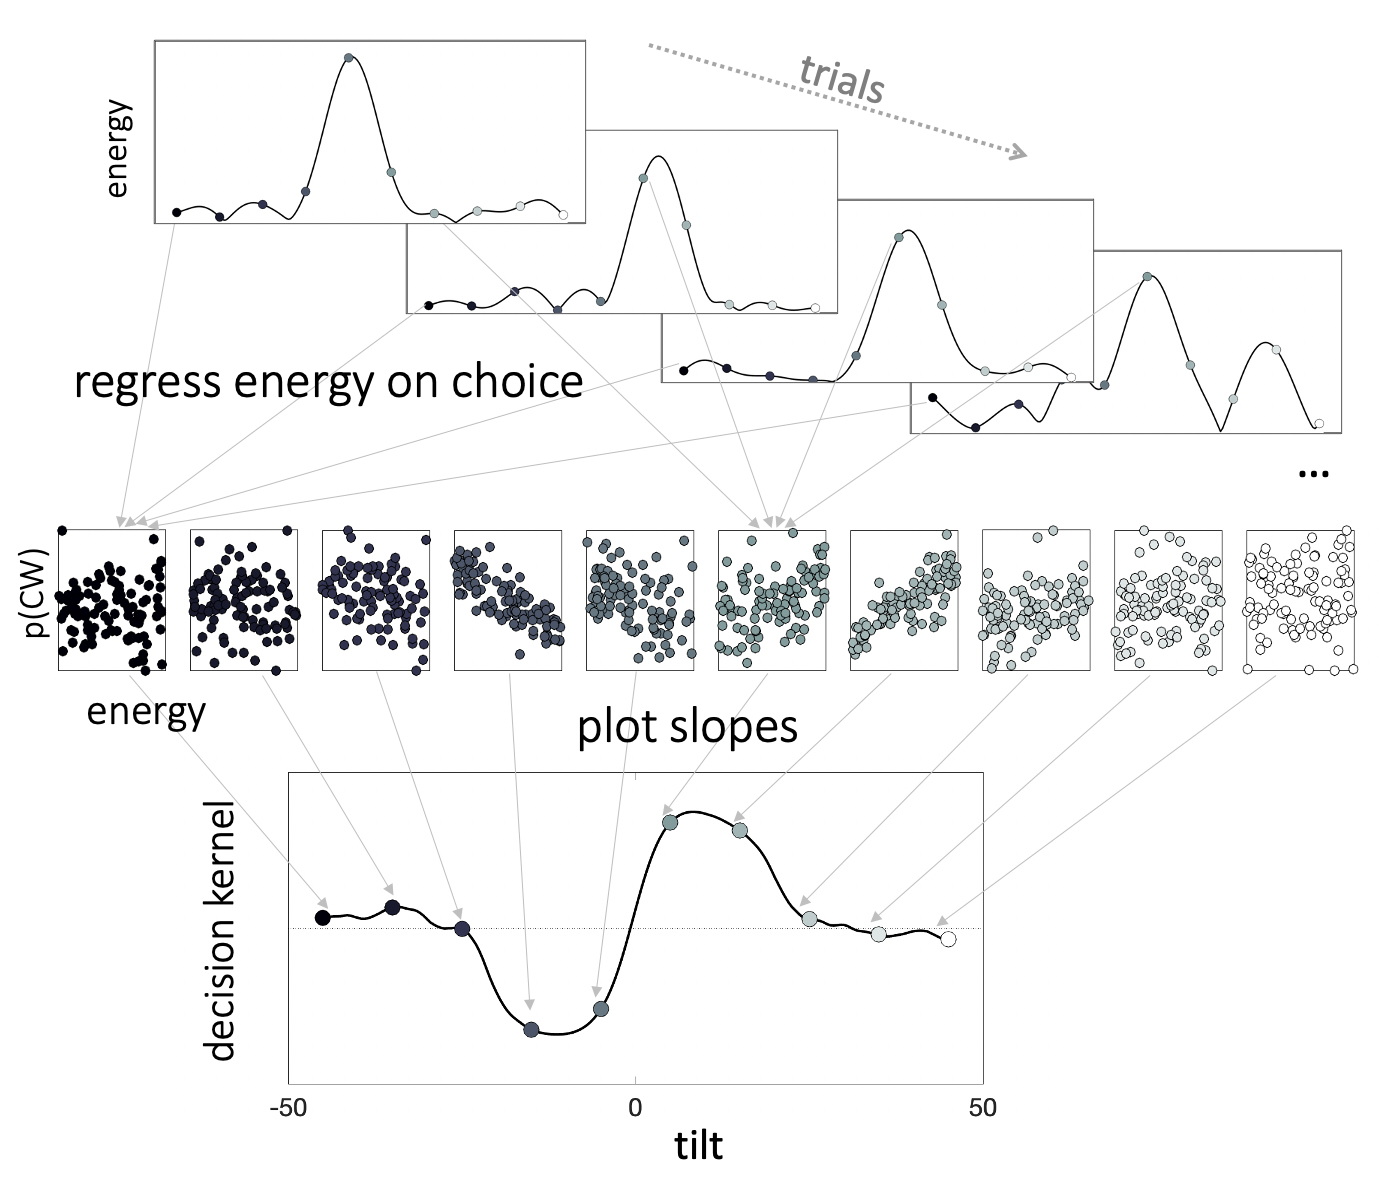
\includegraphics[width=0.8\linewidth]{figures/distr-methods-kernels} 

}

\caption[Reverse correlation analysis, Decision kernels]{Decision kernels. We regressed choices ($p(CW)$) on $z$-scored stimulus energy via separate binomial regressions in each orientation bin. The resulting beta coefficients make up the decision kernel. Thus, the decision kernel indexes the relationship between energy at a given orientation and choice. Positive kernel values suggest that the more a stimulus resembles a Gabor patch of that orientation, the more likely is a participant to make a clockwise choice.}\label{fig:distr-methods-kernels}
\end{figure}

Next, we related fluctuations in energy at each orientation in each trial to participant choices to calculate the decision kernel, i.e.~estimate of the latent function mapping stimulus features on choice (Fig. \ref{fig:distr-methods-kernels}). We did this via a series of parallel binomial regressions, one per each filter orientation, with participant choice (CW or CCW) as the outcome variable and target energy \(E(T_i|\theta)\), standardized within each orientation bin as a \(z\) score, as the predictor variable. The resulting beta coefficients capture the relationship between choice and energy at each orientation, and when plotted together constitute the decision kernel. The reverse correlation approach we describe has been used previously to investigate the effects of feature expectation and attention, as well as spatial attention to target stimuli on choice sensitivity \autocite{wyart2012,barbot2014,cheadle2015}.

In addition to the kernel quantifying the relationship between target energy and choice, we calculated a kernel quantifying the direct effect of the distractor energy on choice (as in the independent model). We estimated the distractor influence by adding distractor energy as a competitive regressor in the model above. We assessed the independent effect of the distractor on choices by testing whether the average absolute values of the distractor kernel deviate from zero at different angles relative to the category boundary. To reduce the number of multiple comparisons, we divided orientation space into angles near the decision boundary (\(|\theta|<22.5\)°) and angles far from the boundary (\(|\theta|>22.5\)°) and averaged the absolute value of the decision kernel within those two bins. Our choice of median split of orientation space was guided by simulations of the theoretical decision kernels (i.e.~simulated responses based on ground truth tilt corrupted by Gaussian noise). We compared the resulting kernel values in the two bins across participants to zero via a single sample \(t\) test.

\hypertarget{kernel-decomposition}{%
\subparagraph{Kernel Decomposition}\label{kernel-decomposition}}

The decision kernel is smooth, so statistical tests conducted at different orientation bins are not independent. To tackle this issue, we reduced the dimensionality of the data via singular value decomposition (SVD). This approach allowed us to derive a set of basis functions (components) from the data itself, and to assess their relative weighing in driving choices. We carried out SVD on a matrix containing the energy profiles of all stimuli, both targets and distractors, from the experiment. The rows of the matrix indexed individual stimuli and the columns indexed orientation bins. The SVD analysis produced a set of components and assigned component scores for each stimulus, which correspond to the variance in the stimulus explained by a given component.

Next, we identified the (number of) components \(V^i\) which explained 95\% of the variance in the data and assessed which of them contained information about the tilt of the stimulus relative the decision boundary via visual inspection. We then used the component scores \(U^i\) for the tilt-informative component(s) of the target and distractor stimuli as predictor variables in a regression model. The model was analogous to the regression model identified through the stepwise algorithm. The only difference was that we used the component scores for the target \(U_T^i\) and distractor \(U_D^i\) instead of their angular offsets, \(\theta_T\) and \(\theta_D\), as predictor variables.

\hypertarget{data-code-availability-statement-1}{%
\subsubsection{Data \& Code Availability Statement}\label{data-code-availability-statement-1}}

All data and code to reproduce the analyses are available in the OSF repository (\url{https://osf.io/54rf2/}) for this project.

\hypertarget{results-3}{%
\subsection{Results}\label{results-3}}

\hypertarget{regression-results}{%
\subsubsection{Regression Results}\label{regression-results}}

\begin{figure}

{\centering 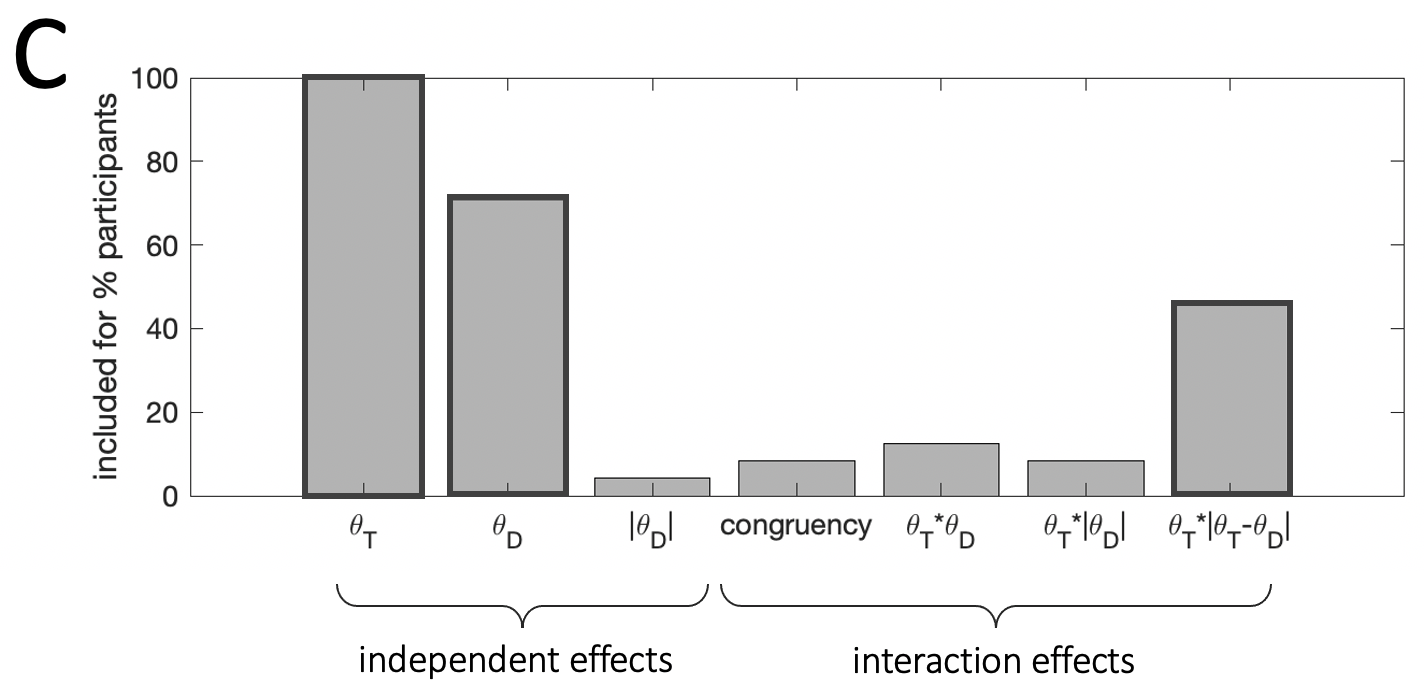
\includegraphics[width=0.8\linewidth]{figures/distr-stepwise-a} 

}

\caption[Experiment 1, Stepwise regression results]{Results from stepwise regressions estimated individually for each participant in the experiment. Bar height indicates the percentage of participants for whom a parameter was included in the final model. Darker bar outlines indicate predictors we included in the final model.}\label{fig:distr-stepwise-a}
\end{figure}

Fig. \ref{fig:distr-stepwise-a} illustrates the proportion of participants whose data was best explained by a model including each of the predictor variables we considered. The model variant that best fit the human data among the candidates we considered was the following:
\begin{equation}
y = \beta_0 + \beta_1\theta_T + \beta_2\theta_D + \beta_3(\theta_T\cdot|\theta_T-\theta_D|)
\label{eq:reg-stepwise}
\end{equation}

This model provided a better explanation of human choices compared to models that included a different functional form for the interaction \(f(\theta_T|\theta_D)\). It also provided a better fit to models that omitted either the independent \(\theta_D\) or interaction effect \(f(\theta_T|\theta_D)\) of the distractor. Bayesian model selection on cross-validated model log likelihoods produced exceedance probabilities of \(p=0.80\) and \(p=0.99\) for this model over an independent effect only model (i.e.~\(\beta_3=0\)) and over an interaction effect only model (i.e.~\(\beta_2=0\)), respectively.

In Eq. \eqref{eq:reg-stepwise} the coefficients \(\beta_1\) and \(\beta_2\) encode the influence (weight) of the target and distractor on choice. The third coefficient \(\beta_3\) encodes the influence of the target-distractor interaction. The functional form of the interaction term indicates a consistency bias -- the influence of the target on choices depends on the degree of consistency between the target and distractor features. That is, choice sensitivity to \(\theta_T\) varies with the similarity between \(\theta_T\) and \(\theta_D\).

\begin{figure}

{\centering 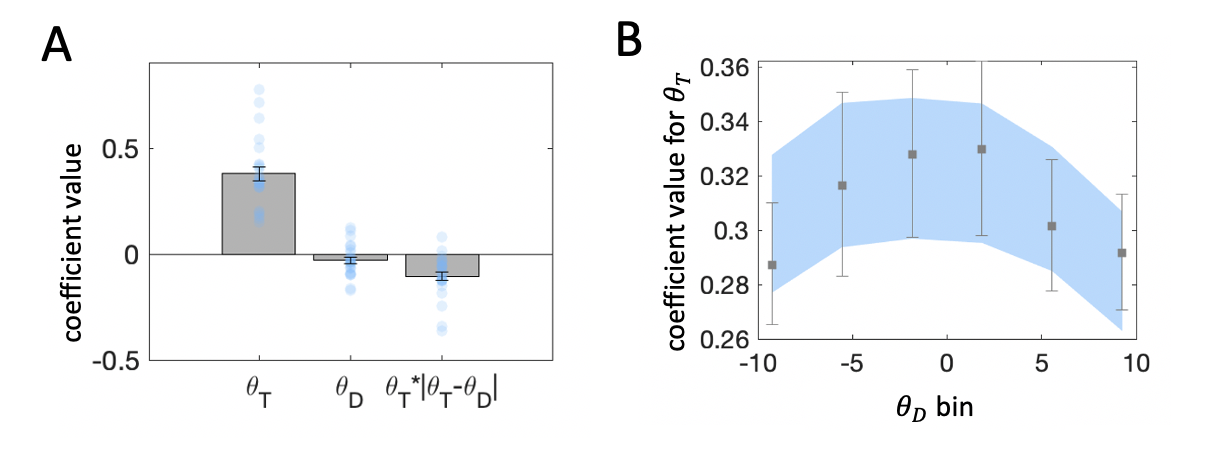
\includegraphics[width=1\linewidth]{figures/distr-regr-a} 

}

\caption[Experiment 1, Regression results]{$\textbf{A:}$ Beta coefficients from regression of choices on target and distractor orientation. Note that the interaction term is divided by 10, to ensure that unit changes in each predictor variable are reported in consistent terms. Grey bars denote averages, error bars denote standard error of the mean, blue dots represent individual participants. $\textbf{B:}$ Beta coefficients for target orientation from binned regressions. Distractor orientation was divided in 6 equally spaced bins. Within each bin we estimated a binomial regression of choices on target orientation. Grey squares denote regression with human choice as the outcome variable, and error bars denote standard error of the mean. Blue region denotes standard error from the same regression, but with choice estimates derived from the regression model (from panel A) fit to human data.}\label{fig:distr-regr-a}
\end{figure}

The best-fitting coefficients \(\beta_1\), \(\beta_2\) and \(\beta_3\) are shown in Fig. \ref{fig:distr-regr-a}a. Firstly, \(\theta_T\) holds significant sway over decisions (\(t_{23}=11.41\), \(p<0.001\)). This is expected because participants were instructed to discriminate the target item. Secondly, the effect of consistency, indexed by \(\beta_3\), was statistically significant at the group level (\(t_{23}=-5.09\), \(p<0.001\)). The negative sign of the coefficient means that the influence of the target on choices was greater when the target-distractor consistency was greater (i.e.~a positive consistency bias).

Thirdly, the effect of \(\theta_D\) was more variable. It appears that the direction of influence of the distractor varied from individual to individual (\(\beta_2 = -0.03 \pm 0.075\)) and a \(t\) test conducted on \(\beta_2\) at the group level failed to reach significance at an \(\alpha\) level of \(.05\), (\(t_{23}=-1.99\), \(p=0.06\)). Although this coefficient was nonsignificant at the group level, the fits of the regression model to data from individual participants suggested that the inclusion of \(\theta_D\) was warranted by the variance it explained.

Fig. \ref{fig:distr-regr-a}b illustrates the results of the binned regression analysis estimating the influence of the target on choices across different distractor values. Sensitivity to the target was reduced for more extreme distractor orientations, across both clockwise and counterclockwise orientations. This finding is expected from the consistency effect, because target and distractor are necessarily more different on average when one of them is at the extreme. This pattern of results is also captured by the predicted choices from the stepwise regression-identified model (Eq. \eqref{eq:reg-stepwise}).

\begin{figure}
 
 {\centering 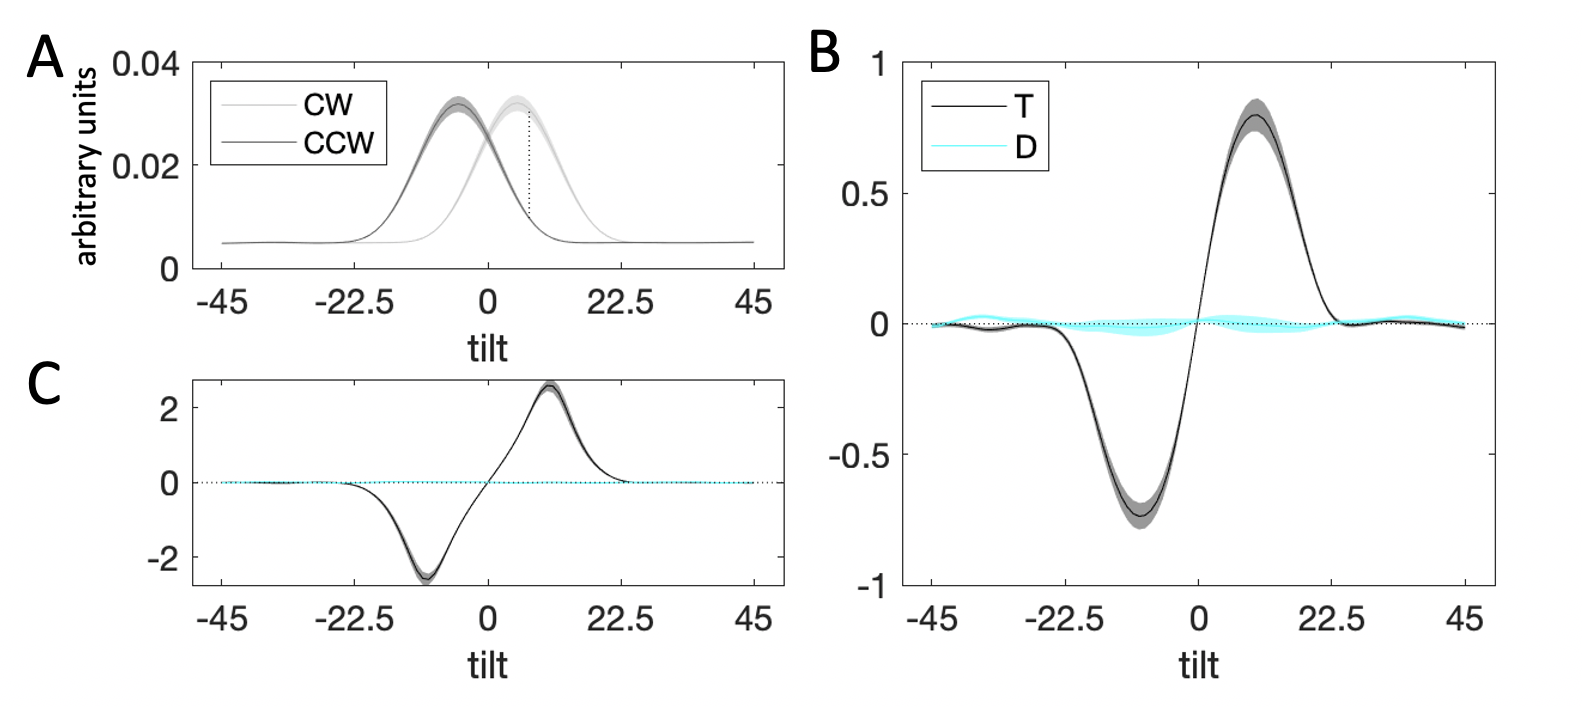
\includegraphics[width=1\linewidth]{figures/distr-kernels-a} 
 
 }
 
 \caption[Experiment 1, Decision kernel results]{Decision kernel results. $\textbf{A:}$ Average stimulus energy profiles. Dark grey curve denotes CCW stimuli, light grey curve -- CW stimuli. Shaded regions correspond to M±SEM. The dashed line denotes maximum signal-to-noise ratio between the distribution for CW and CCW stimuli. $\textbf{B:}$ Decision kernel based on participant choices. Black curve denotes the kernel for the target stimulus, cyan curve -- the kernel for the distractor. Shaded regions correspond to M±SEM. $\textbf{C:}$ Decision kernel based on ground truth stimulus tilts. Black curve denotes the kernel for the target stimulus, cyan curve -- the kernel for the distractor. Shaded regions correspond to M±SEM.}\label{fig:distr-kernels-a}
 \end{figure}

\hypertarget{reverse-correlation-1}{%
\subsubsection{Reverse Correlation}\label{reverse-correlation-1}}

Fig. \ref{fig:distr-kernels-a}b illustrates the decision kernel for the target (black curve) and distractor (cyan line) stimuli averaged over all trials of the experiment. Positive kernel values indicate that an increase in energy at a given orientation is associated with higher probability of responding CW and negative kernel values -- with responding CCW. The peak of the target kernel is on the CW side of orientation space, close to the maximum signal-to-noise ratio of the CW and CCW energy distributions (Fig. \ref{fig:distr-kernels-a}a, dashed line). Note that the kernel tapers towards zero beyond the range of -10° and 10° degrees from which stimulus orientations were sampled. A statistical test confirmed that while the average absolute value of the target kernel was significantly different from zero at orientations close to the decision boundary (i.e.~\(|\theta|<22.5\)°, \(t_{23}=15.57\), \(p<0.001\)), it was not so at orientations far from the decision boundary (i.e.~\(|\theta|>22.5\)°, \(t_{23}=1.78\), \(p=0.09\)). This pattern is also present in a decision kernel calculated based on the ground truth (whether the true stimulus orientation is CW/CCW) rather than participant responses (Fig. \ref{fig:distr-kernels-a}c, near the boundary: \(t_{23}=17.20\), \(p<0.001\), far from the boundary: \(t_{23}=0.99\), \(p=0.33\)).

In Fig. \ref{fig:distr-kernels-a}b, it can be seen that the decision kernel for the distractor was completely flat throughout orientation space. A statistical test on the average of the absolute values of the distractor kernel near the decision boundary (\(t_{23}=0.16\), \(p=0.87\)) and far from the boundary (\(t_{23}=-0.54\), \(p=0.59\)) confirmed that the kernel for the distractor did not deviate from zero. This is consistent with the fact that on its own, the angular offset of the distractor had an inconsistent impact on choices (\(\beta_2\) in the Eq. \eqref{eq:reg-stepwise} regression).

To assess the interaction effect of the distractor, we next turn to the SVD results. The top 4 components derived from the target and distractor stimuli on each trial, which collectively accounted for 96\% of the variance in filter energy (the first component captured 75\% and the second -- 16\%), are shown in Fig. \ref{fig:distr-svd-a}a. Of these 4 components, only component 2 had a different profile for the CW and CCW side of orientation space. Components 1, 3 and 4 were symmetric around the decision boundary. To confirm this intuition, we examined the component scores for each of the 4 components. A negative component score means that the variance in the stimulus is best captured by a mirror image of the component, flipped around the horizontal axis. In line with our visual inspection observations, on average, stimulus scores associated with components 1, 3 and 4 did not differ across CW and CCW oriented stimuli. By contrast, the stimulus scores for the second component appear to contain information pertaining to the tilt of the stimulus -- they were predominantly positive for CW stimuli, and predominantly negative for CCW stimuli. Thus, we chose to use component 2 for our kernel regression analyses.

We regressed participant choices on the stimulus scores for the second component for the target \(U_T^2\) and distractor \(U_D^2\) on each trial, following the Eq. \eqref{eq:reg-stepwise} regression model:
\begin{equation}
y = \beta_0 + \beta_1U_T^2 + \beta_2U_D^2 + \beta_3(U_T^2\cdot|U_T^2-U_D^2|)
\label{eq:reg-svd}
\end{equation}

\begin{figure}

{\centering 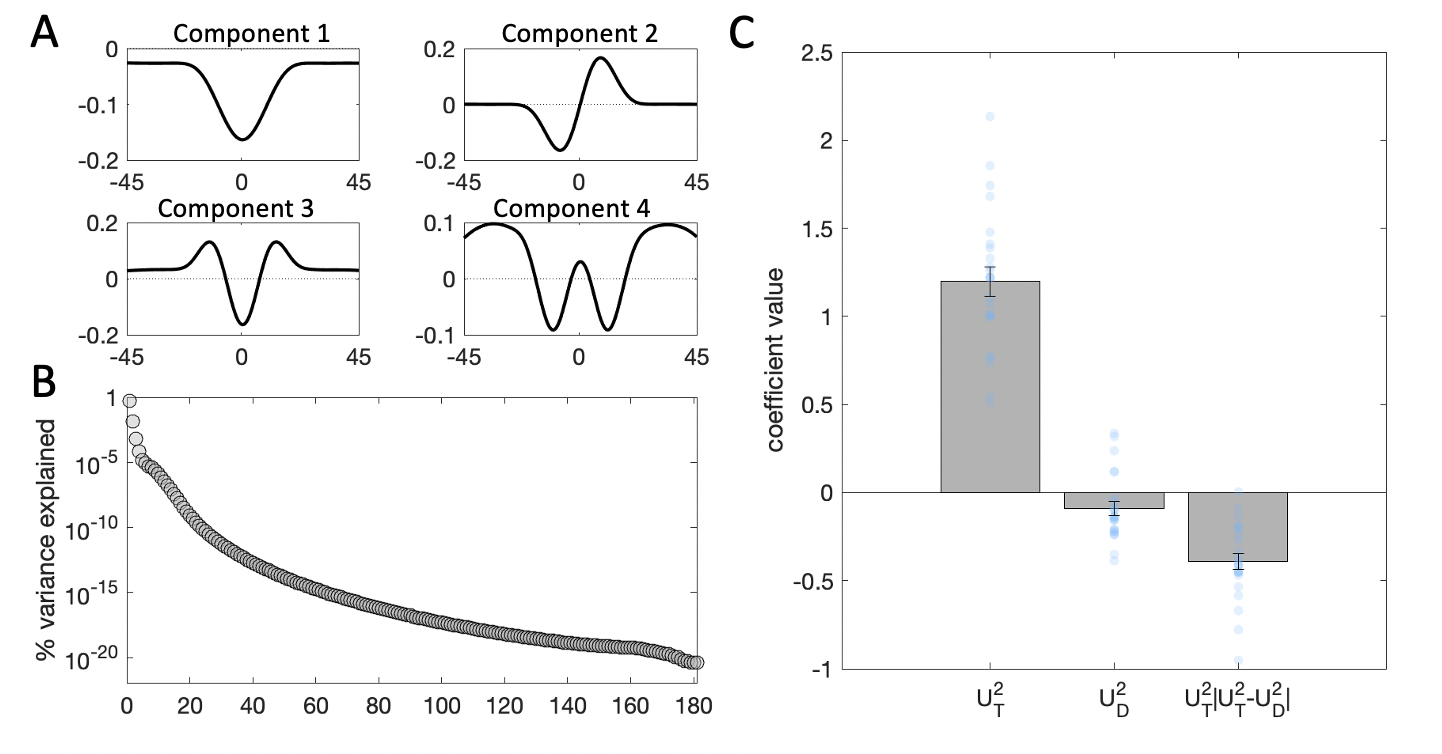
\includegraphics[width=1\linewidth]{figures/distr-svd-a} 

}

\caption[Experiment 1, Kernal decomposition results]{Kernel decomposition results. $\textbf{A:}$ Illustration of the first four components yielded by singular value decomposition (SVD). $\textbf{B:}$ Percentage of variance in the stimulus energy profile explained by each of the SVD components. Note that the y-axis is in logarithmic scale. $\textbf{C:}$ Beta coefficients from a binomial regression of participant choices on stimulus scores for the second component and interactions with distractor signals. Grey bars denote averages, error bars denote standard error of the mean, blue dots represent individual participants.}\label{fig:distr-svd-a}
\end{figure}

Thus, the coefficient \(\beta_1\) reflects the independent effect of the target energy profile (as captured by component 2) on choices, \(\beta_2\) -- the independent effect of the distractor profile, and \(\beta_3\) -- the modulatory (interaction) effect of the distractor on sensitivity to the target, based on the consistency between target and distractor profiles. As expected, the main effect of the target profile on choices was strongly positive (\(t_{23}=14.67\), \(p<0.001\)). In this more sensitive analysis, however, distractor profiles now exerted a small direct repulsive effect on choices (\(t_{23}=-2.34\), \(p=0.03\)). Moreover, as expected from the analyses above, the distractor profile modulated the relationship between target profiles and choices (\(t_{23}=-8.80\), \(p<0.001\)), such that the more consistent the target and distractor profile, the stronger the relationship between target profile and choice.

\hypertarget{interim-discussion-2}{%
\subsection{Interim Discussion}\label{interim-discussion-2}}

Taken together, the results from both our classic and reverse correlation analyses suggest that the effect of distraction is primarily interactive, i.e.~distractors modulate choices by virtue of the way they interact with targets. There may also be a more idiosyncratic independent effect of the distractor on choice. However, this effect was much weaker than the interactive effect and indeed nonsignificant on the group level in our classical regression analysis. The independent distractor effect identified in the reverse correlation analysis was repulsive, meaning that it pushed choices away from the orientation indicated by the distractor. We take these data to mean that the primary way in which distractors influences choices is interactive rather than independent.

\hypertarget{experiment-2}{%
\section{Experiment 2}\label{experiment-2}}

We next asked whether the interactive effect of distraction operates at the perceptual level or at the decision level. That is, is the contextual influence of the distractor driven by its sensory features or by its decision information? The interaction model has been proposed to operate across both sensory domains \autocite[e.g.~in visual cortex,][]{kapadia1995} and in more abstract decision processes \autocite[e.g.~about value-based information,][]{louie2013}. Our task features a low level visual property (orientation), suggesting that interactions between raw sensory information could be driving the effect. However, sensory level interactions have been documented at comparably closer locations in retinotopic space \autocite{polat1994} relative to our task here, which positioned target and distractor in opposite visual hemifields. Thus, the effects we observe might instead be driven by interactions at later stages of processing of decision inputs.

To disentangle the perceptual and decision level information in our task, we orthogonalized the decision boundaries for target and distractor stimuli. Thus, in Experiment 2, target and distractor stimuli that share the same tilt relative to their respective boundary would be offset by 90° in terms of their raw tilts. We reasoned that if the contextual influence of the distractor occurred at the perceptual level and thus depended on similarity in terms of raw tilt, then the interaction effect would be null in Experiment 2 where this similarity is all but destroyed. Hence, any interaction effect that survives this manipulation must be due to encoding of information at the decision level (i.e.~similarity of tilt relative to the boundary).

We analyzed the data from Experiment 2 in the frame of reference of the decision boundary. That is, we used stimulus tilt relative to the respective boundary rather than raw stimulus orientation in all our analyses. This allowed us to first, avoid wrap around effects in sensory similarity due to the circular nature of orientation space, and second, compare directly the magnitude of the \emph{decision level} interaction effects between Experiments 1 and 2. If we see equivalent consistency effects in both experiments, this would indicate that the influence of the distractor occurs at the decision level.

\hypertarget{methods-4}{%
\subsection{Methods}\label{methods-4}}

\hypertarget{participants-2}{%
\subsubsection{Participants}\label{participants-2}}

Thirty-two participants (aged 24 ±4.75) took part in Experiment 2. Eight participants were excluded from the main analyses as the accuracy of their responses for one of the possible stimulus locations was at chance level (defined as in Experiment 1). The study received ethical approval from the Central University Research Ethics Committee at the University of Oxford (approval reference number: R51752/RE002). All participants provided written informed consent and were compensated £10 per hour for their time.

\hypertarget{apparatus-1}{%
\subsubsection{Apparatus}\label{apparatus-1}}

Participants were seated in a dark room approximately 60cm away from a computer monitor (60Hz refresh rate, 1080x1290 resolution, 23' Dell LCD) with linearized output light intensities. As in Experiment 1, visual stimuli were created and presented with Psychophysics Toolbox Version 3 \autocite[PsychToolbox-3,][]{brainard1997} for MATLAB.

\hypertarget{stimuli-1}{%
\subsubsection{Stimuli}\label{stimuli-1}}

Experimental stimuli were as in Experiment 1; the only difference was in stimulus orientation. In one of the two stimulus locations, the decision boundary was vertical like in Experiment 1. In the other location, the decision boundary was horizontal. In line with this, Gabor pattern orientation was drawn from a uniform distribution with range --10° to 10° offset from vertical or horizontal for the two respective stimulus locations. The average value of the contrast ratio for the noise in the stimuli produced by the staircase across participants was 0.42. This relatively higher signal contrast in Experiment 2 (versus 0.32 in Experiment 1) indicates that, on average, participants found the task harder when using two different decision boundaries. This is in line with the relatively higher number of participants excluded due to chance-level performance in this experiment (8 versus 2 in Experiment 1).

\hypertarget{experimental-procedure-1}{%
\subsubsection{Experimental Procedure}\label{experimental-procedure-1}}

\begin{figure}

{\centering 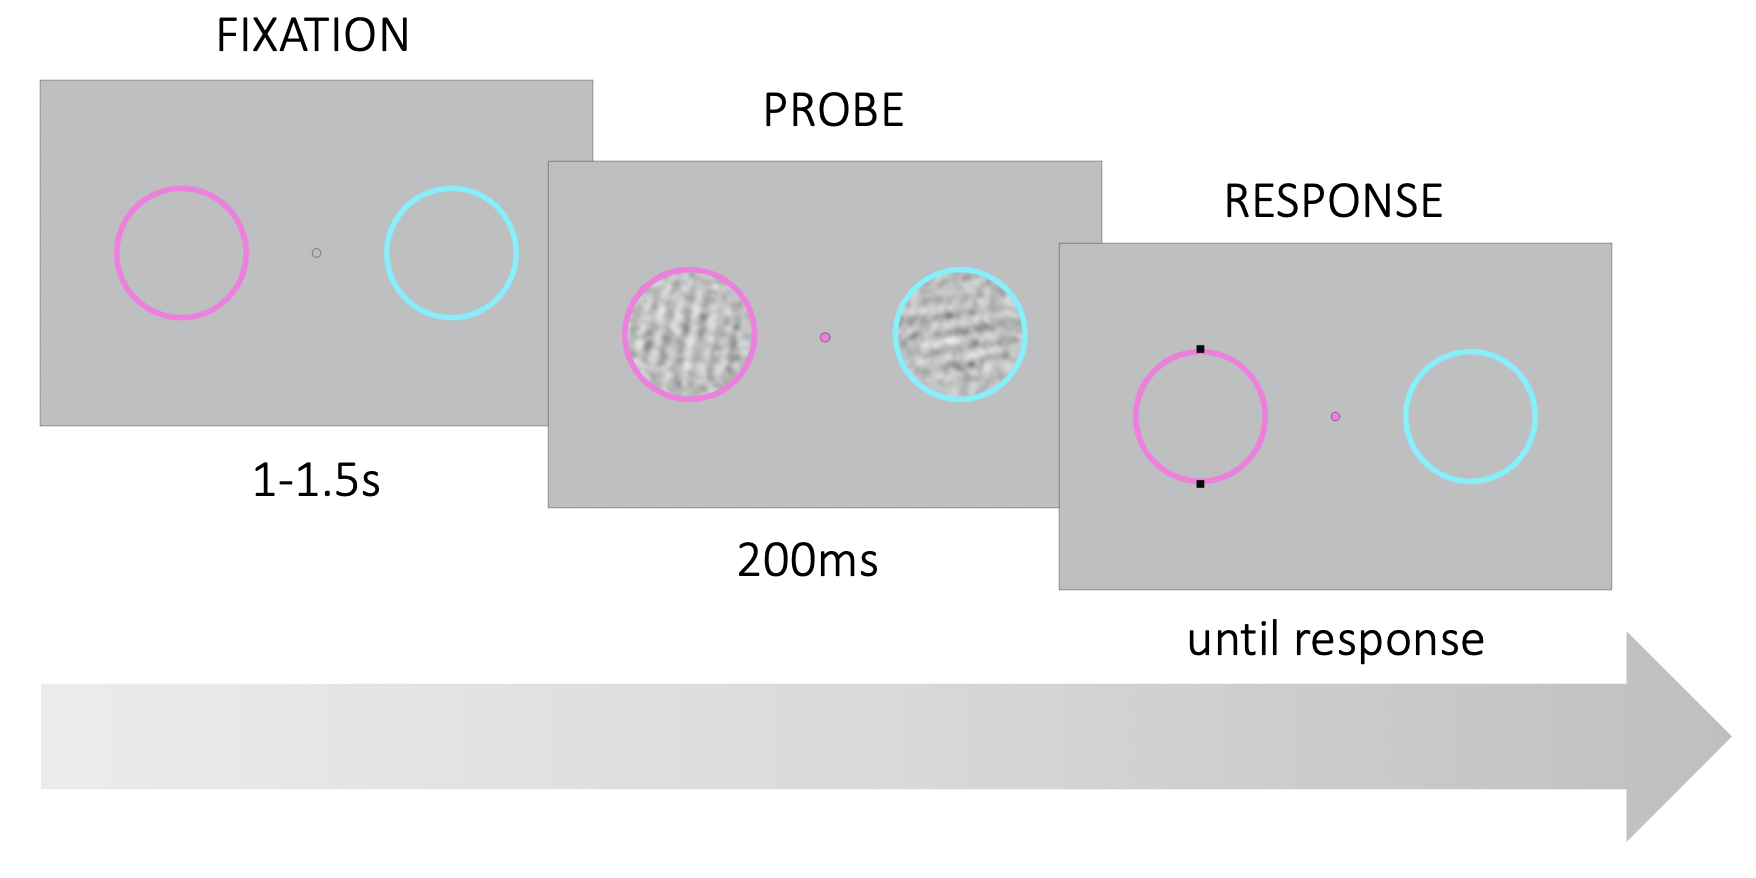
\includegraphics[width=1\linewidth]{figures/distr-trial-b} 

}

\caption[Experiment 2, Trial structure]{Trial structure followed Experiment 1. However, the two colored rings had different reference orientations. In the example here, the decision boundary for the pink ring was vertical, and horizontal for the cyan ring.}\label{fig:distr-trial-b}
\end{figure}

The experimental procedure followed that of Experiment 1 (Fig. \ref{fig:distr-trial-b}). The only difference between the two experiments was in decision boundaries. In Experiment 2, for one of the colored rings the decision boundary was vertical, and for the other -- horizontal. The decision boundaries were fixed for the duration of the experiment and ring-boundary combinations were counterbalanced between participants. Participants were reminded of the relevant decision boundary by two dots (oriented vertically or horizontally) overlayed over the target ring on each trial.

\hypertarget{analyses-2}{%
\subsubsection{Analyses}\label{analyses-2}}

We followed the same analysis plan as for Experiment 1. As stimulus features were coded as angular offset from the relevant decision boundary, all analyses were conducted in decision space rather than in the raw sensory orientation space.

\hypertarget{data-code-availability-statement-2}{%
\subsubsection{Data \& Code Availability Statement}\label{data-code-availability-statement-2}}

All data and code to reproduce the analyses are available in the OSF repository (\url{https://osf.io/54rf2/}) for this project.

\hypertarget{results-4}{%
\subsection{Results}\label{results-4}}

\hypertarget{regression-results-1}{%
\subsubsection{Regression Results}\label{regression-results-1}}

\begin{figure}

{\centering 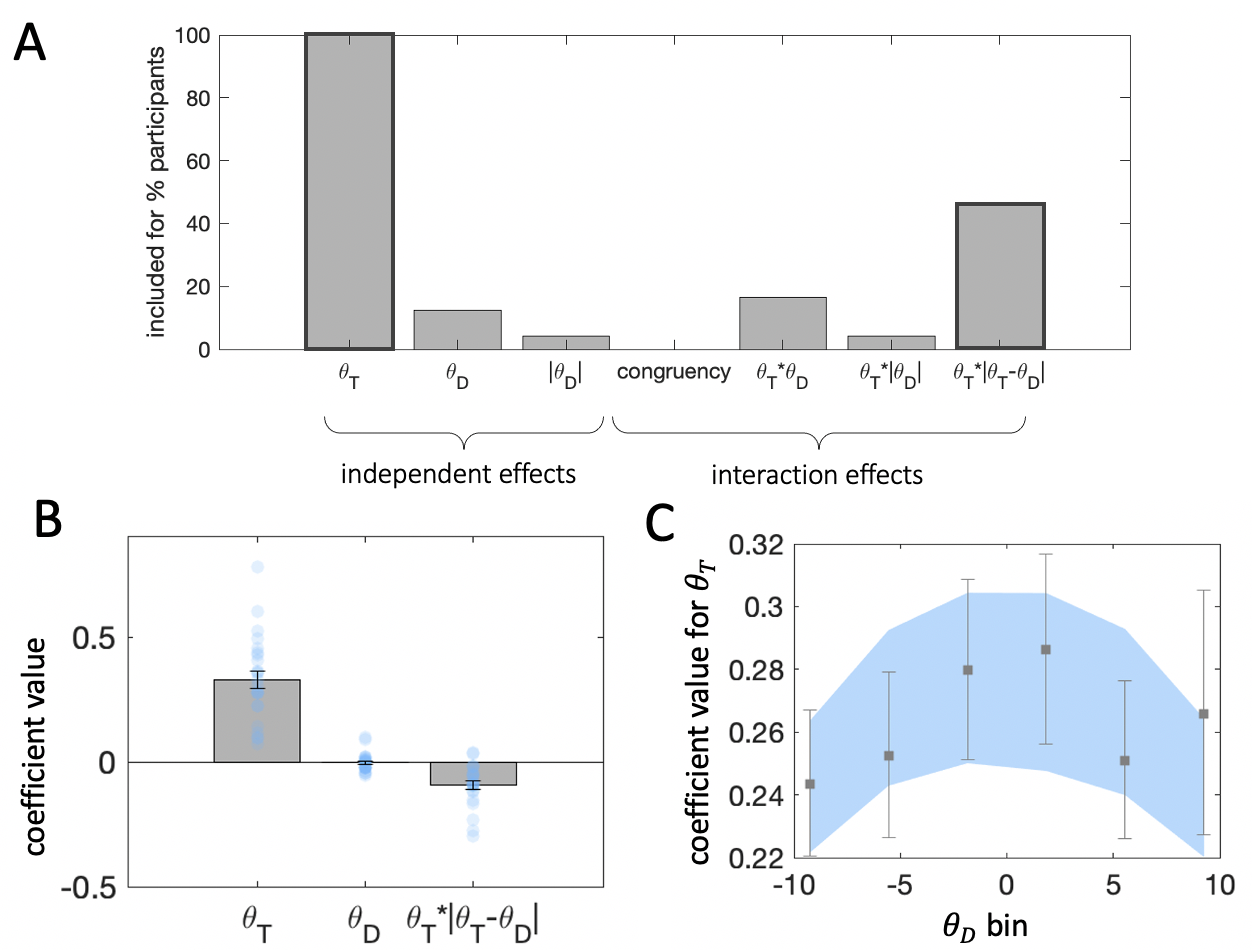
\includegraphics[width=1\linewidth]{figures/distr-regr-b} 

}

\caption[Experiment 2, Regression results]{Regression results. Plots are as in Experiment 1. $\textbf{A:}$ Results from stepwise regressions estimated individually for each participant in the experiment. Darker bar outlines indicate predictors we included in the final model. $\textbf{B:}$ Beta coefficients from regression of choices on target and distractor orientation. $\textbf{C:}$ Beta coefficients for target orientation from binned regressions.}\label{fig:distr-regr-b}
\end{figure}

Fig. \ref{fig:distr-regr-b}a illustrates the results of the stepwise regression on participant choices. Interestingly, while the independent effect of the target and the interaction effect of distraction mirrored the findings from Experiment 1, the independent effect of the distractor explained a sufficient amount of variance to be included in the final model for only 3 out of 24 participants. Thus, the best fitting model for the choice data in Experiment 2 was:
\begin{equation}
y = \beta_0 + \beta_1\theta_T + \beta_3(\theta_T\cdot|\theta_T-\theta_D|)
\label{eq:reg-stepwise-b}
\end{equation}

As expected, the target had a strong positive influence on choices (\(t_{23}=9.89\), \(p<0.001\)) and the coefficient for the interaction effect of distraction was negative (\(t_{23}=-5.13\), \(p<0.001\)). For consistency with Experiment 1, we also report the results for the Eq. \eqref{eq:reg-stepwise} model (Fig. \ref{fig:distr-regr-b}b). The results for the target (\(t_{23}=9.40\), \(p<0.001\)) and the interaction effect of distraction (\(t_{23}=-5.43\), \(p<0.001\)) follow the same pattern. The coefficient for the independent effect of the distractor failed to reach statistical significance (\(t_{23}=-0.51\), \(p=0.62\)). Thus, in this experiment, the direction of the independent influence of the distractor again varied from individual to individual (\(\beta_2=-0.004 \pm 0.037\)), however, its inclusion in the model was not warranted by the amount of variance it explained in participant choices.

As can be seen from Fig. \ref{fig:distr-regr-b}c, the results of the binned regression analysis followed closely those from Experiment 1. Across both participant and regression model-predicted choices, sensitivity to the target was reduced for more extreme distractor orientations, across both clockwise and counterclockwise orientations. This pattern of results is in line with the observed consistency bias.

\hypertarget{reverse-correlation-2}{%
\subsubsection{Reverse Correlation}\label{reverse-correlation-2}}

\begin{figure}

{\centering 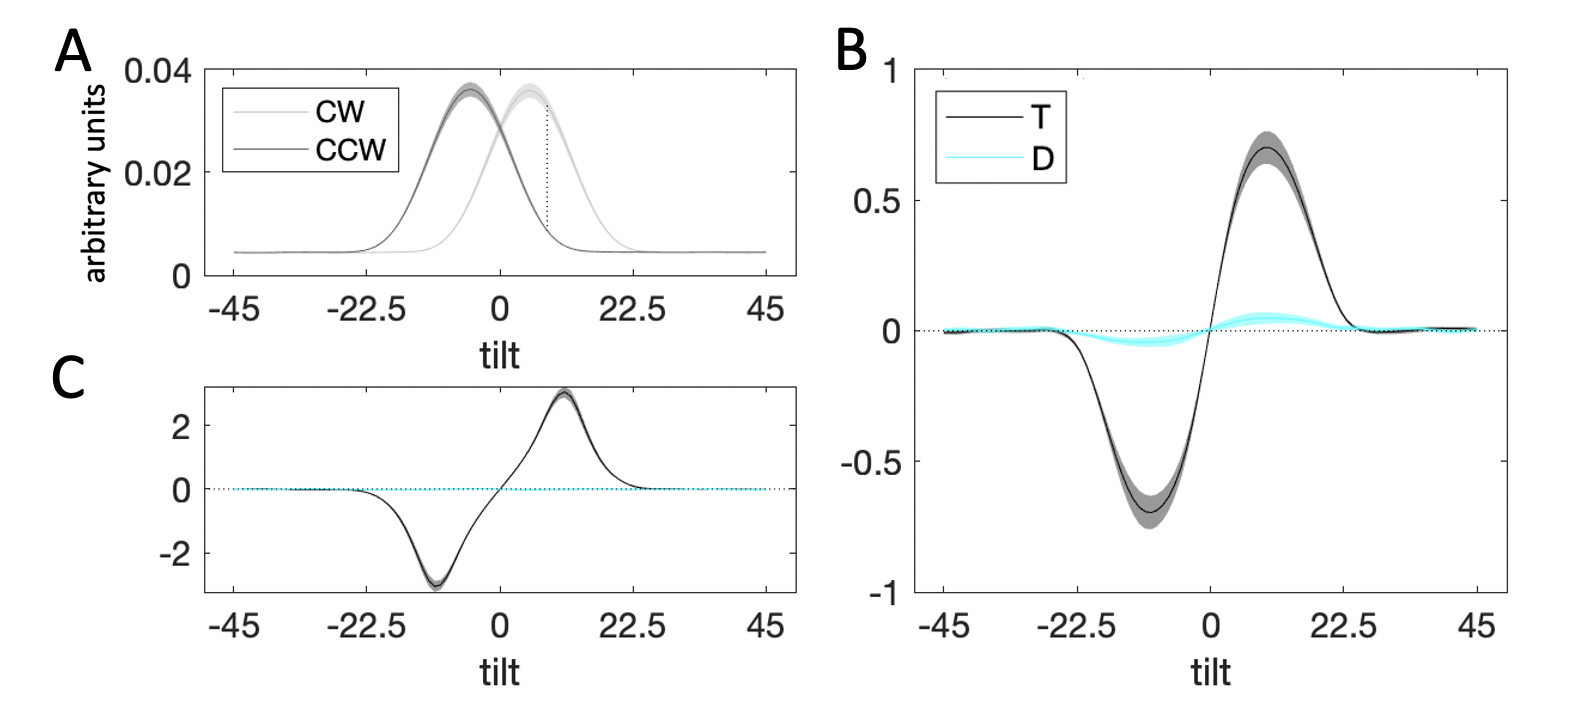
\includegraphics[width=1\linewidth]{figures/distr-kernels-b} 

}

\caption[Experiment 2, Decision kernel results]{Decision kernel results. Plots are as in Experiment 1. $\textbf{A:}$ Average stimulus energy profiles. $\textbf{B:}$ Decision kernel based on participant choices. $\textbf{C:}$ Decision kernel based on ground truth stimulus tilts.}\label{fig:distr-kernels-b}
\end{figure}

Fig. \ref{fig:distr-kernels-b}b illustrates the decision kernel for the target and distractor. The target kernel follows the same pattern as in Experiment 1, with a peak on the CW side of feature space and a trough on the CCW side. Again, it tapered off to zero for angles away from the decision boundary (close to the boundary: \(t_{23}=13.06\), \(p<0.0001\), far from the boundary: \(t_{23}=1.27\), \(p=0.22\)). Interestingly, the distractor kernel appears slightly peaked in a way that follows the target kernel. Indeed, the average absolute value of the kernel at orientations close to the category boundary was significantly different from zero (\(t_{23}=2.47\), \(p=0.02\)), but further from the category boundary it was nonsignificant (\(t_{23}=0.17\), \(p=0.86\)). This suggests that participant choices were attracted, albeit rather weakly, towards the signal-like energy in the distractor.

\begin{figure}

{\centering 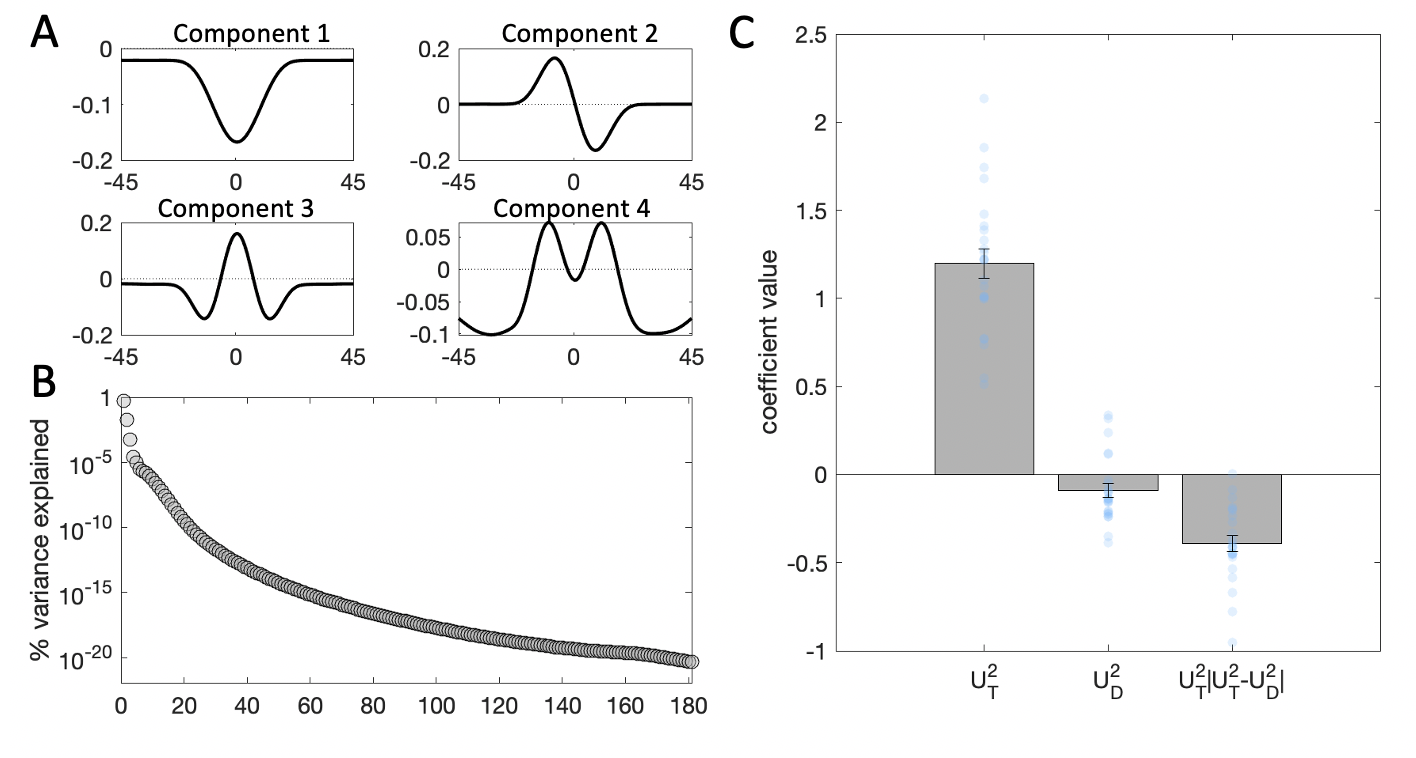
\includegraphics[width=1\linewidth]{figures/distr-svd-b} 

}

\caption[Experiment 2, Kernel decomposition results]{Kernel results. Plots are as in Experiment 1. $\textbf{A:}$ Illustration of the first four components yielded by SVD. Note that the second component is a mirror image of the component resulting from Experiment 1. For ease of interpretability and consistency between the two experiments, we flipped the sign of the component scores for component 2 in the following analyses. $\textbf{B:}$ Percentage of variance in the stimulus energy profile explained by each of the SVD components. $\textbf{C:}$ Beta coefficients from a binomial regression of participant choices on stimulus scores for the second component and interactions with distractor signals. Grey bars denote averages, error bars denote standard error of the mean, blue dots represent individual participants.}\label{fig:distr-svd-b}
\end{figure}

The SVD regression analysis yielded analogous components as in Experiment 1 (Fig. \ref{fig:distr-svd-b}a-b). This is perhaps unsurprising, as we followed the same stimulus generation procedure. The second component, however, was flipped compared to the second component derived from the stimuli in Experiment 1, suggesting that here, positive component scores would be associated with CCW stimuli, and negative component scores with CW stimuli. Thus, for ease of interpretability and consistency with Experiment 1, we multiplied \(U^2\) by \((-1)\) prior to fitting the Eq. \eqref{eq:reg-svd} regression model (Fig. \ref{fig:distr-svd-b}c). The results followed those from Experiment 1. We found a positive independent effect of the target (\(t_{23}=10.84\), \(p<0.001\)) and a negative interaction effect of target-distractor consistency (\(t_{23}=-7.94\), \(p<0.001\)). The independent effect of the distractor failed to reach statistical significance in this analysis, where, unlike in the simple \(t\) test above, we controlled for the interaction effect of the distractor (\(t_{23}=-1.19\), \(p=0.24\)).

\hypertarget{interim-discussion-2}{%
\subsection{Interim Discussion}\label{interim-discussion-2}}

Overall, the results of Experiment 2 replicate the main findings from Experiment 1. The effect of target-distractor consistency was similar across the two experiments despite the fact that here the decision boundaries for target and distractor were orthogonal (horizontal and vertical). This implies that the relevant features for target and distractor interact at the decision rather than at the perceptual level, i.e.~at a stage in which they have been placed in a frame of reference that is relative to the decision boundary. The independent effect of the distractor was more elusive. Unlike Experiment 1, here the independent effect of the distractor was not included in the best fitting model. It also produced nonsignificant coefficients in regression analyses based on distractor tilt and distractor energy. Interestingly, while in Experiment 1 there were suggestions that the distractor may exert a weak repulsive influence on choices, here a small attraction effect was apparent in the distractor kernel.

Perhaps counter-intuitively, this pattern of results is actually in line with the direct repulsive influence of the distractor reported in Experiment 1 if the direct effect of the distractor occurs at the perceptual level. As analyses for Experiment 2 were carried out on the tilt offset of the two stimuli relative to two orthogonal boundaries, inputs that are close in decision space (e.g.~tilt offsets 10° and 9° = 1° distance in decision space) are actually further in sensory space (respectively 10° and 99° = 89° distance in orientation space) compared to inputs that are more distanced in decision space (e.g.~tilt offsets 10° and -9° = 19° distance in decision space, respectively 10° and 81° = 71° distance in orientation space). Thus, to interpret these results in the same frame of reference as the findings from Experiment 1, we should swap the sign of the effect. The relatively weaker direct effect here could be owing to the fact that target-distractor tilt pairs used in Experiment 2 were much more distant in orientation space compared to those in Experiment 1.

\hypertarget{experiment-3}{%
\section{Experiment 3}\label{experiment-3}}

Focusing attention on a decision-relevant location promotes target processing at the expense of distractors, and leads to heightened accuracy and faster reaction times \autocite{posner1980,hawkins1990,carrasco2011}. This naturally raises the question of how the interactive effect of distraction described here changes when targets are, or are not, the focus of spatial attention. In Experiment 3, thus, we manipulated spatial attention by probabilistically cueing participants to focus on either the target or distractor stimulus in order to asses interactions with distraction.

\hypertarget{methods-5}{%
\subsection{Methods}\label{methods-5}}

\hypertarget{participants-3}{%
\subsubsection{Participants}\label{participants-3}}

Twenty participants (aged 24.3 ±3.69) took part in the Experiment 3. The study received ethical approval from the Central University Research Ethics Committee at the University of Oxford (approval reference number: R64927/RE001). All participants provided written informed consent and were compensated £10 per hour for their time.

\hypertarget{apparatus-2}{%
\subsubsection{Apparatus}\label{apparatus-2}}

Participants were seated in a dark room approximately 60cm away from a computer monitor (60Hz refresh rate, 1024x768 resolution, 17' LCD) with linearized output light intensities. Visual stimuli were created and presented with Psychophysics Toolbox Version 3 \autocite[PsychToolbox-3,][]{brainard1997} for MATLAB. Throughout the experiment, participants' eye gaze position was monitored via eye-tracking using SR Research EyeLink 1000.

\hypertarget{stimuli-2}{%
\subsubsection{Stimuli}\label{stimuli-2}}

Experimental stimuli were generated as described in Experiment 1.

\hypertarget{experimental-procedure-2}{%
\subsubsection{Experimental Procedure}\label{experimental-procedure-2}}

Each participant completed the experiment in a single session, lasting approximately three hours. The experimental session consisted of 2 training mini-blocks of 50 trials each, an adaptive staircase and 9 test blocks of 200 trials each with a short break midway through each test block. The 2 training mini-blocks served to familiarize the participant with the task and the staircase followed the same procedure as in Experiments 1 and 2.

\begin{figure}

{\centering 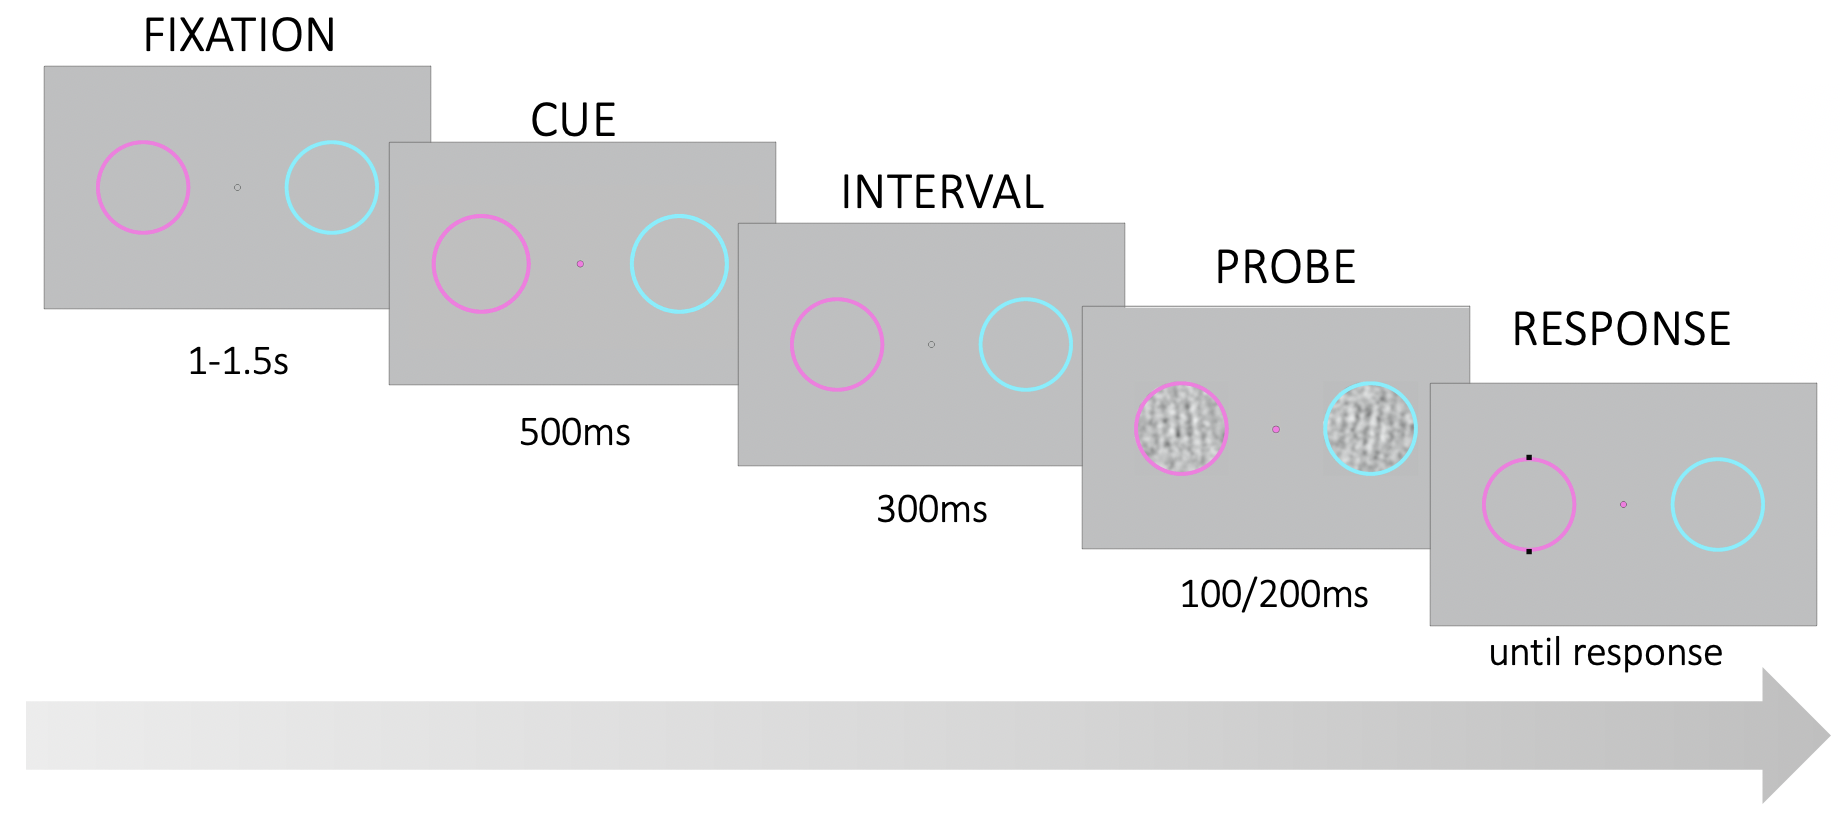
\includegraphics[width=1\linewidth]{figures/distr-trial-c} 

}

\caption[Experiment 3, Trial structure]{Trial structure followed Experiment 1. However, here, 800ms prior to stimulus presentation, the fixation point assumed the color of the ring which was more likely to be probed for 500ms. Note that on each trial stimulus duration was randomly determined as either 100ms or 200ms.}\label{fig:distr-trial-c}
\end{figure}

We adjusted the trial sequence in the test blocks to manipulate spatial attention via a spatial cue component (Fig. \ref{fig:distr-trial-c}). The cue provided information about which stimulus was more likely to be the target. In 2 of the test blocks, the cue was neutral, and thus, trials were in practice equivalent to Experiment 1 (other than some small differences in trial timing). Participants were informed at the start of the neutral blocks that the cue would not be informative and the color of the fixation point (white) reflected this. In the remaining 7 blocks, the cue assumed the color of the ring which was more likely (70\%) to be probed.

Each trial began with the probabilistic cue -- the fixation point assumed the color of one of the two rings (or white in the neutral condition) for 500ms. 300ms following cue offset, two noisy gratings appeared within the colored rings for either 100ms or 200ms. Stimulus timings were randomized across trials to maximize the effect of cue validity on choice. At stimulus onset, the fixation point assumed the color of one of the two rings until the end of the trial. The color of the fixation point served as the probe indicating which of the two stimuli was the target. At stimulus offset, two dots were overlaid over the target ring. These dots corresponded to the vertical decision boundary relative to which participants had to report the tilt of the target. Participants reported their responses via keyboard presses (left and right arrow keys) and instantaneously received fully informative auditory feedback (correct: high tone, 880Hz and incorrect: low tone, 440Hz). Responses were not accepted on trials where the participant failed to maintain fixation, defined as gaze location further than 2° in radius from fixation. The experimenter remained in the same room as the participant to re-calibrate the eye tracker in between experimental blocks. Auditory feedback was delivered to the participant via headphones.

\hypertarget{analyses-3}{%
\subsubsection{Analyses}\label{analyses-3}}

We adapted the analytic strategy from Experiments 1 and 2, to assess the influence of spatial attention and its interaction with the effect of the distractor.

\hypertarget{manipulation-checks}{%
\paragraph{Manipulation checks}\label{manipulation-checks}}

First, we conducted manipulation checks to confirm that our spatial attention manipulation was successful. We coded each trial in the experiment into three cueing conditions: 1) valid, where the probabilistic cue correctly signaled the target stimulus, 2) invalid, where the probabilistic cue incorrectly signaled the distractor stimulus, and 3) neutral, where the cue provided no information. We compared accuracy rates (converted to log odds to avoid violating the normality assumption) and response times (log transformed to again avoid violating the normality assumption) across these three cueing conditions via a GLM, controlling for the nonindependence of data points from the same observer. We followed up the results of the GLM with pairwise comparisons via \(t\) tests.

\hypertarget{regression-analyses}{%
\paragraph{Regression Analyses}\label{regression-analyses}}

Collapsing across cueing condition, we followed the analytic pipeline from Experiments 1 and 2. To assess interactions with spatial attention, in addition to the predictors identified via the stepwise approach, we added cueing condition as an interaction term to each of the predictors. Valid, neutral and invalid cueing conditions were coded as 1, 0 and -1 respectively.

\hypertarget{reverse-correlation-3}{%
\paragraph{Reverse correlation}\label{reverse-correlation-3}}

We repeated all reverse correlation analyses from Experiments 1 and 2, collapsing across cueing condition. To assess interactions with attention, we plotted kernels for each cueing condition separately. For the SVD regression analyses, we followed the same strategy as above -- we included cueing condition as an interaction term to each of the predictors in the regression model.

\hypertarget{data-code-availability-statement-3}{%
\subsubsection{Data \& Code Availability Statement}\label{data-code-availability-statement-3}}

All data and code to reproduce the analyses are available in the OSF repository (\url{https://osf.io/54rf2/}) for this project.

\hypertarget{results-5}{%
\subsection{Results}\label{results-5}}

\begin{figure}

{\centering 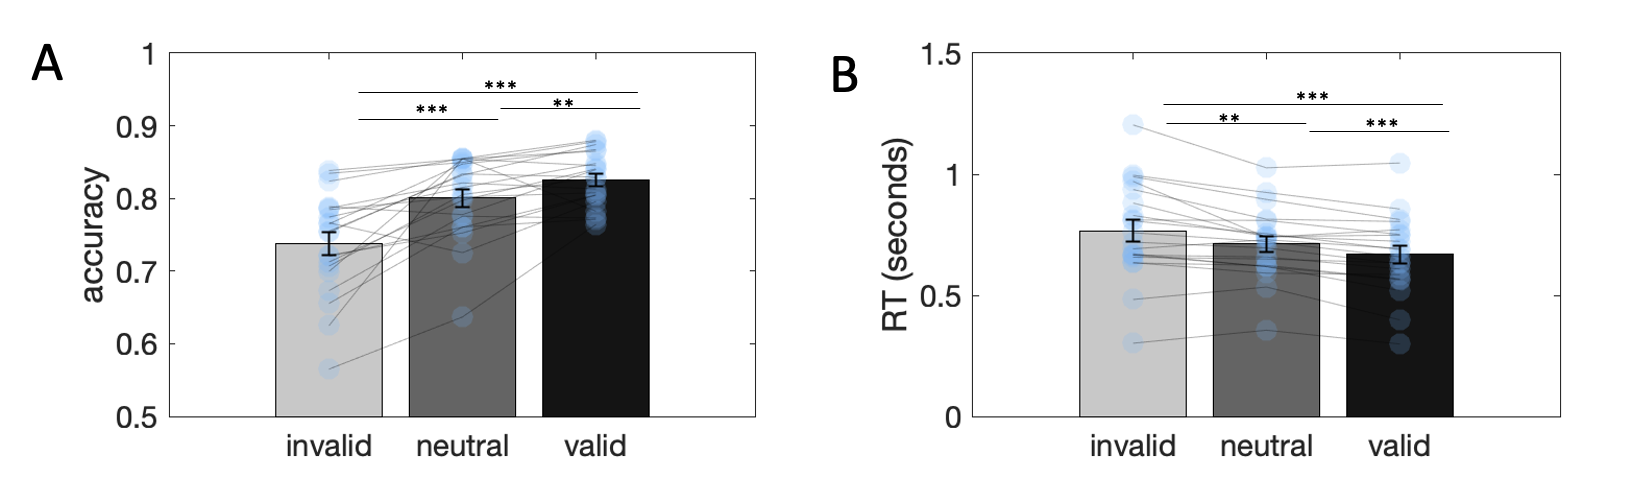
\includegraphics[width=1\linewidth]{figures/distr-man-check} 

}

\caption[Experiment 3, Attention manipulation check]{Attention manipulation check. $\textbf{A:}$ Accuracy across invalid, neutral and valid trials. Statistical tests were performed on odds ratio transformed measures. $\textbf{B:}$ Response times across invalid, neutral and valid trials. Statistical tests were performed on log transformed measures. Stars denote statistical significance: ** = p<0.01, *** = p<0.001.}\label{fig:distr-man-check}
\end{figure}

\hypertarget{manipulation-checks-1}{%
\subsubsection{Manipulation checks}\label{manipulation-checks-1}}

Fig. \ref{fig:distr-man-check} shows accuracy rates and response times across the three cueing conditions. As expected, accuracy was highest for valid trials and lowest for invalid trials, while response times followed the opposite pattern, indicating that our attention manipulation was successful. Log-transformed response time showed a valid \textless{} neutral \textless{} invalid pattern (GLM coefficient \(\beta=-0.07\), \(p<0.0001\); pairwise comparisons: valid \textless{} invalid: \(t_{19}=-8.76\), \(p<0.0001\), valid \textless{} neutral: \(t_{19}=-4.34\), \(p<0.0001\), neutral \textless{} invalid: \(t_{19}=-2.61\), \(p<0.02\)) and accuracy (transformed into log odds) showed a valid \textgreater{} neutral \textgreater{} invalid pattern (GLM coefficient \(\beta=0.26\), \(p<0.0001\); valid \textgreater{} invalid: \(t_{19}=6.07\), \(p<0.0001\), valid \textgreater{} neutral: \(t_{19}=3.00\), \(p<0.01\), neutral \textgreater{} invalid: \(t_{19}=4.82\), \(p<0.0001\)).

\hypertarget{regression-results-2}{%
\subsubsection{Regression Results}\label{regression-results-2}}

\begin{figure}

{\centering 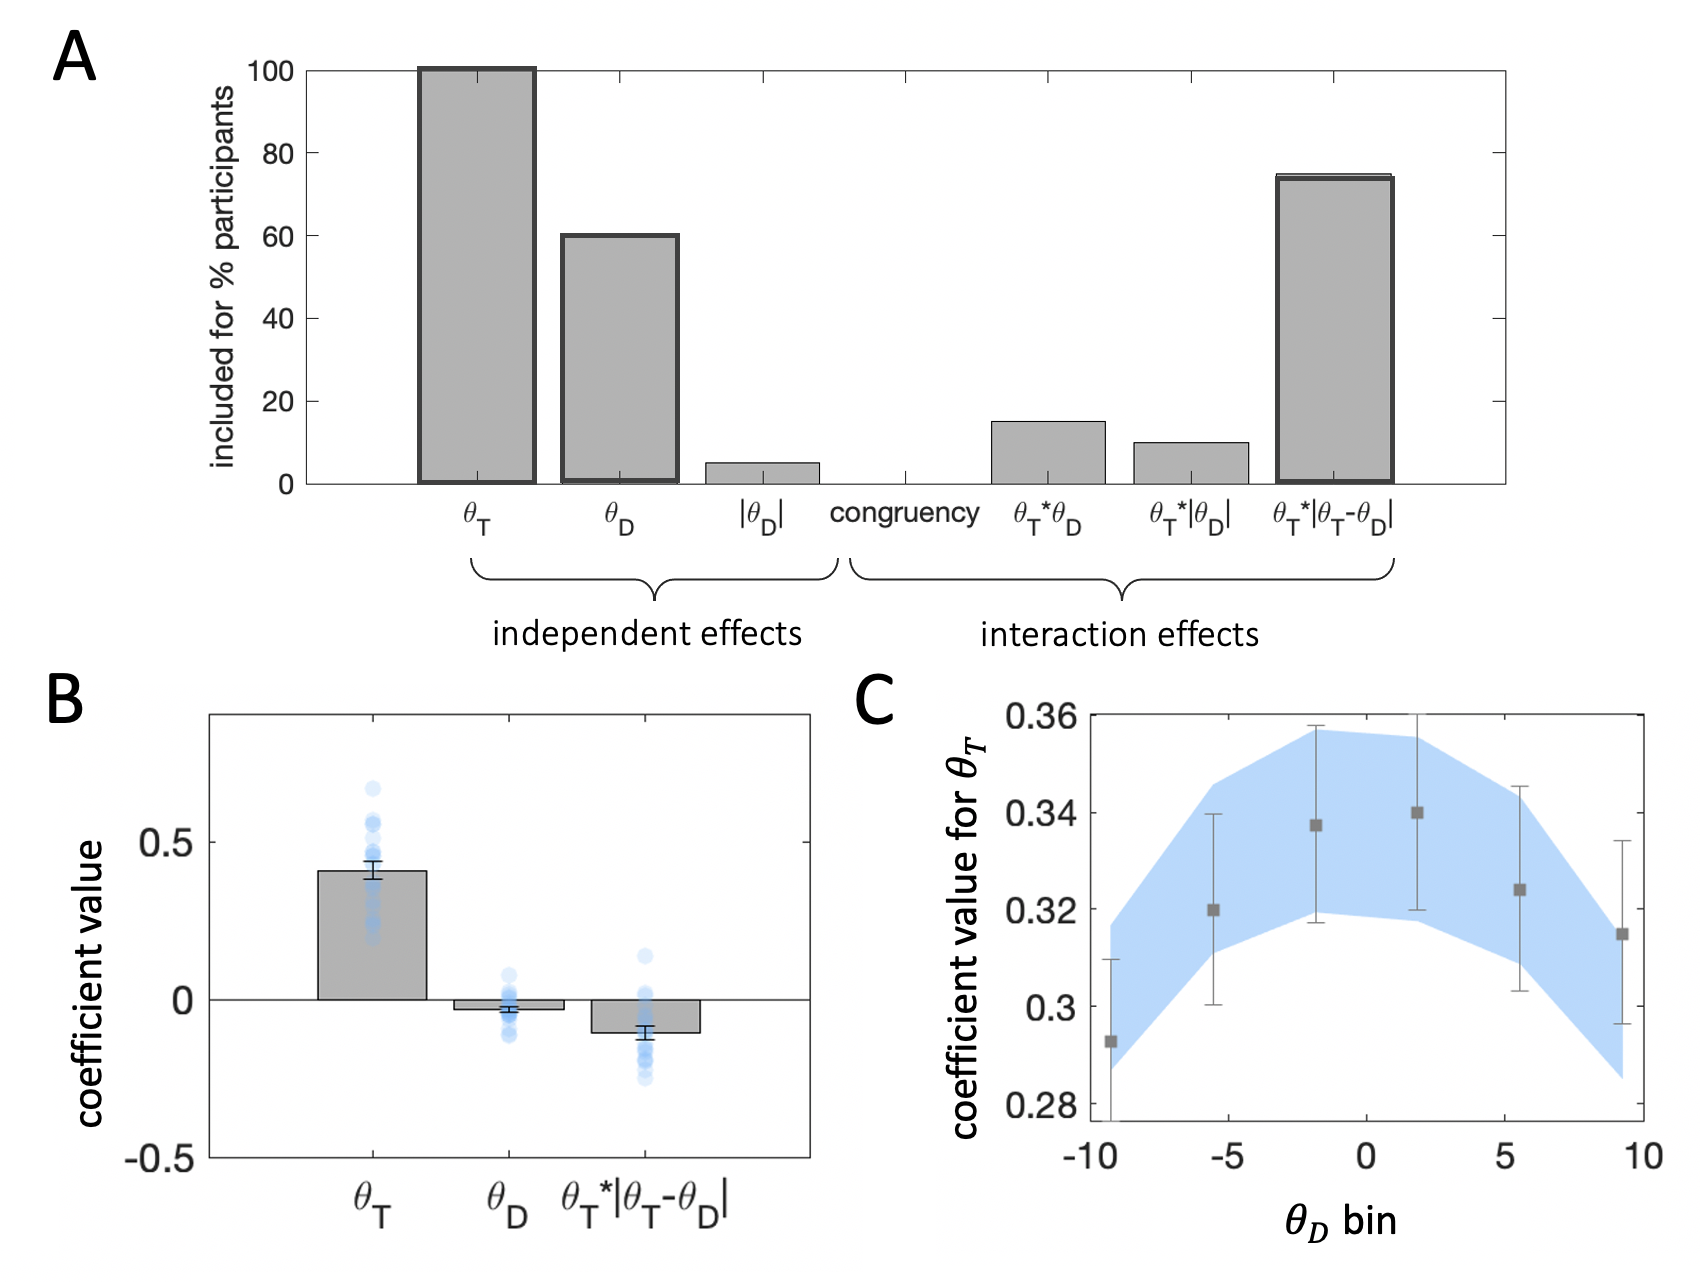
\includegraphics[width=1\linewidth]{figures/distr-regr-c} 

}

\caption[Experiment 3, Regression results]{Regression results collapsing across cueing condition. Plots are as in Experiment 1. $\textbf{A:}$ Results from stepwise regressions estimated individually for each participant in the experiment. Darker bar outlines indicate predictors we included in the final model. $\textbf{B:}$ Beta coefficients from regression of choices on target and distractor orientation. $\textbf{C:}$ Beta coefficients for target orientation from binned regressions.}\label{fig:distr-regr-c}
\end{figure}

First, we attempted to replicate the regression analyses from Experiments 1 and 2 collapsing across cueing condition. As can be seen from Fig. \ref{fig:distr-regr-c}a, the stepwise regression identified the same predictors as in Experiment 1. Fitting Eq. \eqref{eq:reg-stepwise} to the choice data from Experiment 3 replicated the strong sway of targets on choice (\(t_{19}=14.17\), \(p<0.001\)) and the target-distractor consistency effect (\(t_{19}=-5.00\), \(p<0.001\)). Here, the distractor had a statistically significant repulsive effect (\(t_{19}=-3.17\), \(p=0.005\)). The binned regressions produced the same pattern of results as in Experiments 1 and 2. Target sensitivity in participant and model-produced choices was reduced at more extreme distractor orientations, in line with the observed consistency bias.

Next, to assess the impact of target and distractor (and their interaction) under different attentional cueing conditions, we again used logistic regression (Fig. \ref{fig:distr-attention}b), but now including interaction terms with attention (cueing) condition:
\begin{equation}
y = \beta_0 + \beta_1\theta_T + \beta_2\theta_D + \beta_3(\theta_T\cdot|\theta_T-\theta_D|) + \beta_4A\cdot\theta_T + \beta_5A\cdot\theta_D + \beta_6A\cdot(\theta_T\cdot|\theta_T-\theta_D|)
\label{eq:reg-stepwise-att}
\end{equation}

This expression looks a little complicated but in fact builds naturally from Eq. \eqref{eq:reg-stepwise}. The first three terms (associated with \(\beta_1\),\(\beta_2\) and \(\beta_3\)) are identical to those in Eq. \eqref{eq:reg-stepwise}. The final three terms are new predictors that encode the extent to which \(\theta_T\), \(\theta_D\) and their interaction influence choices as a function of cueing validity. In Eq. \eqref{eq:reg-stepwise-att} thus \(A\) is an indicator variable coding cueing validity.

The results for \(\beta_{(1-3)}\) restate those described above (\(\beta_1\): \(t_{19}=13.57\), \(p<0.001\), \(\beta_2\): \(t_{19}=-2.68\), \(p=0.02\), \(\beta_3\): \(t_{19}=-4.69\), \(p<0.001\)). Attention modulated sensitivity to target orientations (\(\beta_4\): \(t_{19}=4.80\), \(p<0.001\)), as expected from previous work in the attention literature. Surprisingly, however, attention did not impact the direct effect of the distractor (\(\beta_5\): \(t_{19}=-1.46\), \(p=0.16\)), nor its modulatory influence on target sensitivity (\(\beta_6\): \(t_{19}=0.71\), \(p=0.49\)).

\begin{figure}

{\centering 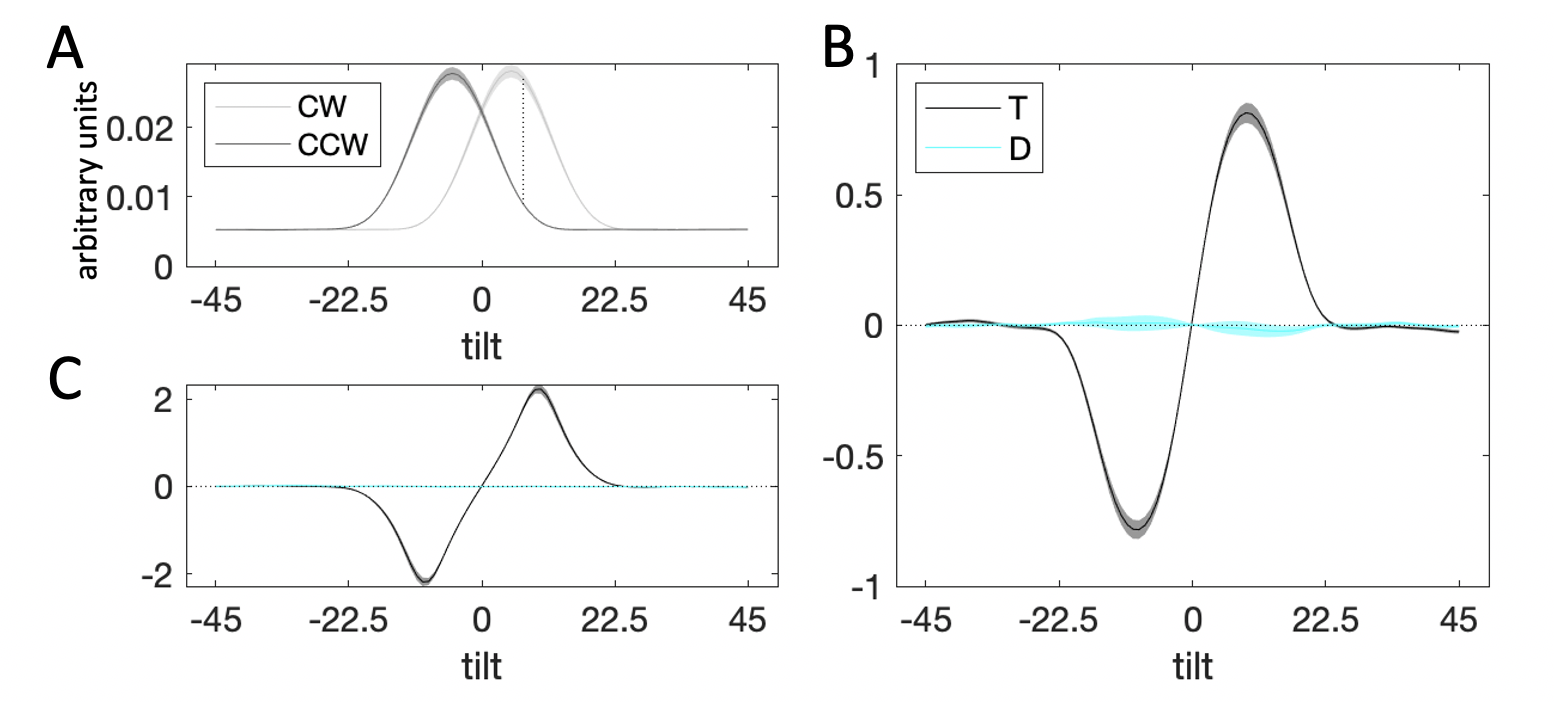
\includegraphics[width=1\linewidth]{figures/distr-kernels-c} 

}

\caption[Experiment 3, Decision kernel results]{Decision kernel results collapsing across cueing condition. Plots are as in Experiment 1. $\textbf{A:}$ Average stimulus energy profiles. $\textbf{B:}$ Decision kernel based on participant choices. $\textbf{C:}$ Decision kernel based on ground truth stimulus tilts.}\label{fig:distr-kernels-c}
\end{figure}

\hypertarget{reverse-correlation-results}{%
\subsubsection{Reverse Correlation Results}\label{reverse-correlation-results}}

Again, we started by attempting to replicate the reverse correlation results from Experiments 1 and 2 collapsing across cueing condition. The kernel results were consistent with those above (Fig. \ref{fig:distr-kernels-c}). The target kernel significantly drove choices close to the category boundary (\(t_{19}=23.80\), \(p<0.001\)) and tapered off to zero for orientations further away from the boundary (\(t_{19}=-1.43\), \(p=0.17\)). The distractor kernel was flat throughout orientation space (near the category boundary: \(t_{19}=-0.55\), \(p=0.59\), far from the category boundary: \(t_{19}=0.09\), \(p=0.92\)).

\begin{figure}

{\centering 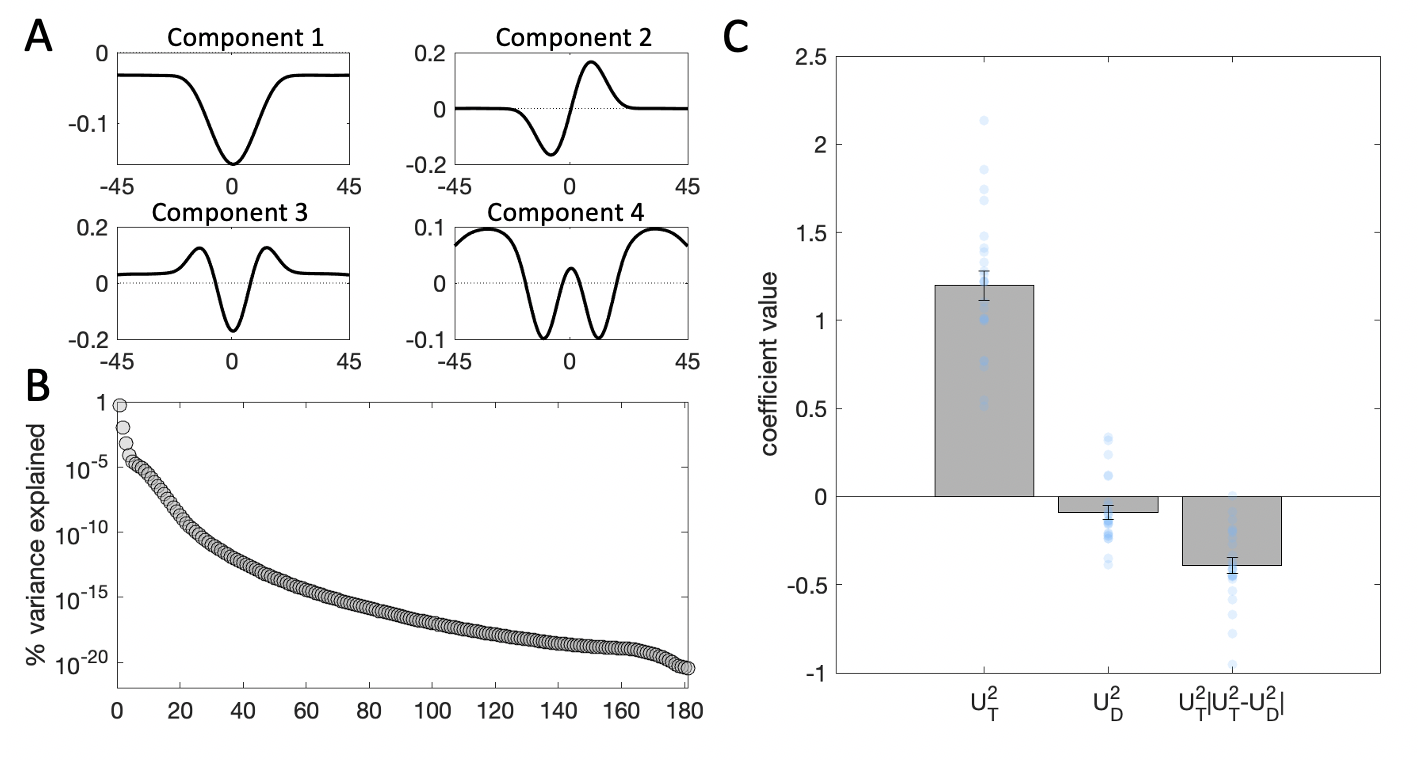
\includegraphics[width=1\linewidth]{figures/distr-svd-c} 

}

\caption[Experiment 3, Kernel decomposition results]{Kernel decomposition results collapsing across cueing condition. Plots are as in Experiment 1.  $\textbf{A:}$ Illustration of the first four components yielded by SVD.  $\textbf{B:}$ Percentage of variance in the stimulus energy profile explained by each of the SVD components.  $\textbf{C:}$ Beta coefficients from a binomial regression of participant choices on stimulus scores for the second component and interactions with distractor signals. Grey bars denote averages, error bars denote standard error of the mean, blue dots represent individual participants.}\label{fig:distr-svd-c}
\end{figure}

The SVD results (Fig. \ref{fig:distr-svd-c}) and the regression based on component 2 replicated the findings from Experiment 1. The direct effect of the target profile on choices was strongly positive (\(t_{19}=18.72\), \(p<0.001\)) and we again observed the interaction effect of the consistency of target and distractor profiles on choice (\(t_{19}=-8.80\), \(p<0.001\)). Like in Experiment 1, we also observed a small direct repulsive effect of the distractor on choices (\(t_{19}=-3.29\), \(p=0.004\)).

Next, we considered these effects under different cueing conditions. Fig. \ref{fig:distr-attention}a shows that there appears to be an attention-induced enhancement of target sensitivity in the decision kernels for the three different attention conditions. To quantitatively assess this, we re-ran the attention-inclusive regression model from Eq. \eqref{eq:reg-stepwise-att} using the scores for component 2 as the predictor variables:
\begin{equation}
y = \beta_0 + \beta_1U_T^2 + \beta_2U_D^2 + \beta_3(U_T^2\cdot|U_T^2-U_D^2|) + \beta_4A\cdot U_T^2 + \beta_4A\cdot U_D^2 + \beta_6A\cdot(U_T^2\cdot|U_T^2-U_D^2|)
\label{eq:reg-svd-att}
\end{equation}

The results of this model replicated the results from the model based on angular offset \(\theta\) (Eq. \eqref{eq:reg-stepwise-att}). The the target profile held a significant sway on decisions (\(\beta_1\): \(t_{19}=17.44\), \(p<0.001\)), the distractor profile exerted a repulsive influence (\(\beta_2\): \(t_{19}=-2.73\), \(p=0.01\)) as well as a negative interactive effect driven by its consistency with the target profile (\(\beta_3\): \(t_{19}=-9.63\), \(p<0.001\)). Crucially, cueing condition modulated sensitivity to the target (\(\beta_4\): \(t_{19}=5.12\), \(p<0.001\)), but had no impact on the direct effect of the distractor (\(\beta_5\): \(t_{19}=-1.66\), \(p=0.14\)), nor its modulatory influence on target sensitivity (\(\beta_6\): \(t_{19}=-1.15\), \(p=0.27\)).

\begin{figure}

{\centering 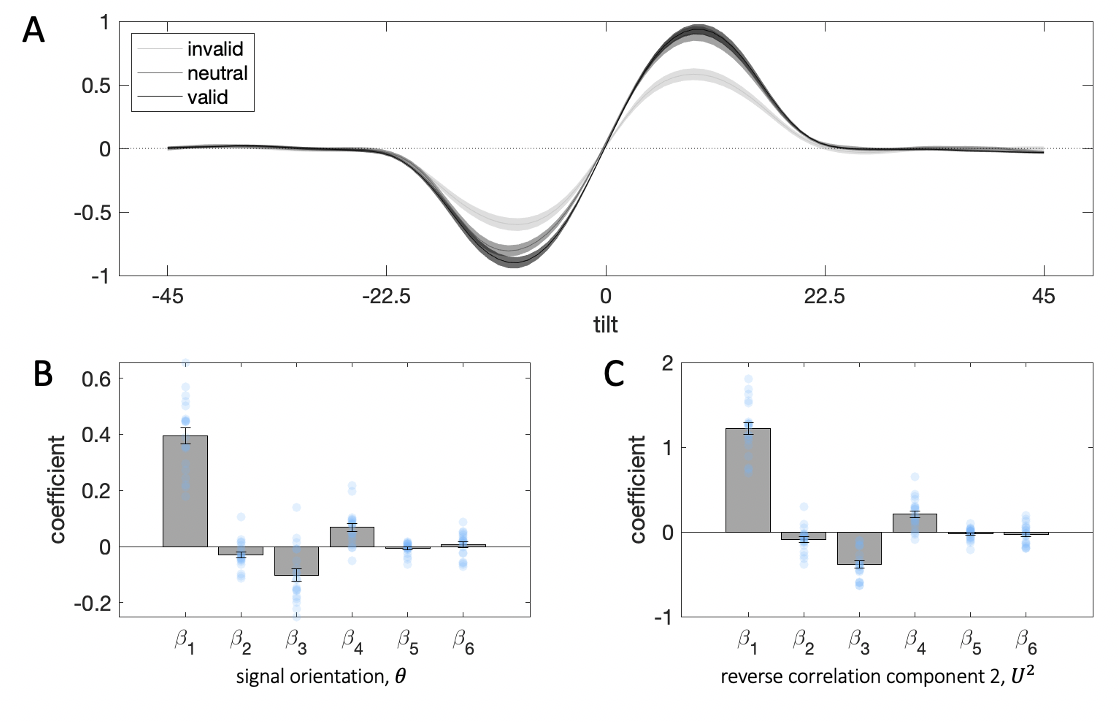
\includegraphics[width=1\linewidth]{figures/distr-attention} 

}

\caption[Experiment 3, Results per cueing condition]{Results per cueing condition. $\textbf{A:}$ Decision kernels for the target kernel in invalid, neutral and valid trials. Lightest grey denotes invalid, mid-grey -- neutral and darkest grey -- valid trials. $\textbf{B:}$ Beta coefficients from a binomial regression on signal orientation. Grey bars denote averages, error bars denote standard error of the mean, blue circles denote individual participants. $\beta_1$ is the coefficient for the target stimulus, $\beta_2$ – the distractor, $\beta_3$ – the interaction between target and the consistency between target and distractor, $\beta_4$ – the interaction between target and cueing condition (coded as -1=invalid, 0=neutral, 1=valid), $\beta_5$ – the interaction between the distractor and cueing condition, $\beta_6$ – the three-way interaction between target, target-distractor consistency and cueing condition. $\textbf{C:}$ As in B, but dependent variables in the regression correspond to the score for SVD component 2 from the reverse correlation analysis.}\label{fig:distr-attention}
\end{figure}

\hypertarget{interim-discussion-3}{%
\subsection{Interim Discussion}\label{interim-discussion-3}}

Collapsing across cueing condition, the results of Experiment 3 again replicate the interactive influence of the distractor. Here, we also observe a direct repulsive influence of distractors on choice, which we detected in only some of the analyses in Experiment 1. The observed contextual effects of irrelevant information do not differ across valid, invalid and neutral trials. This implies that directing attention heightens sensitivity to the imperative target stimulus, but, perhaps counter-intuitively, does not impact the contextual effects of irrelevant information.

\hypertarget{computational-modeling-1}{%
\section{Computational Modeling}\label{computational-modeling-1}}

The regression models above (Eq. \eqref{eq:reg-stepwise}-\eqref{eq:reg-svd-att}) were an analytic tool designed to partition variance in choice between independent predictors (\(\theta_T\) and \(\theta_D\)) and an interaction term \(f(\theta_T|\theta_D)\). However, there is a perhaps more elegant way to model the data, and one that, although closely related, makes more direct links to models of attention and contextual biasing that rely on normalization \autocite{reynolds2009}:
\begin{equation}
y = \frac{(x-\rho\cdot\mu)}{r+\tau\cdot\sigma}
\end{equation}

\begin{figure}

{\centering 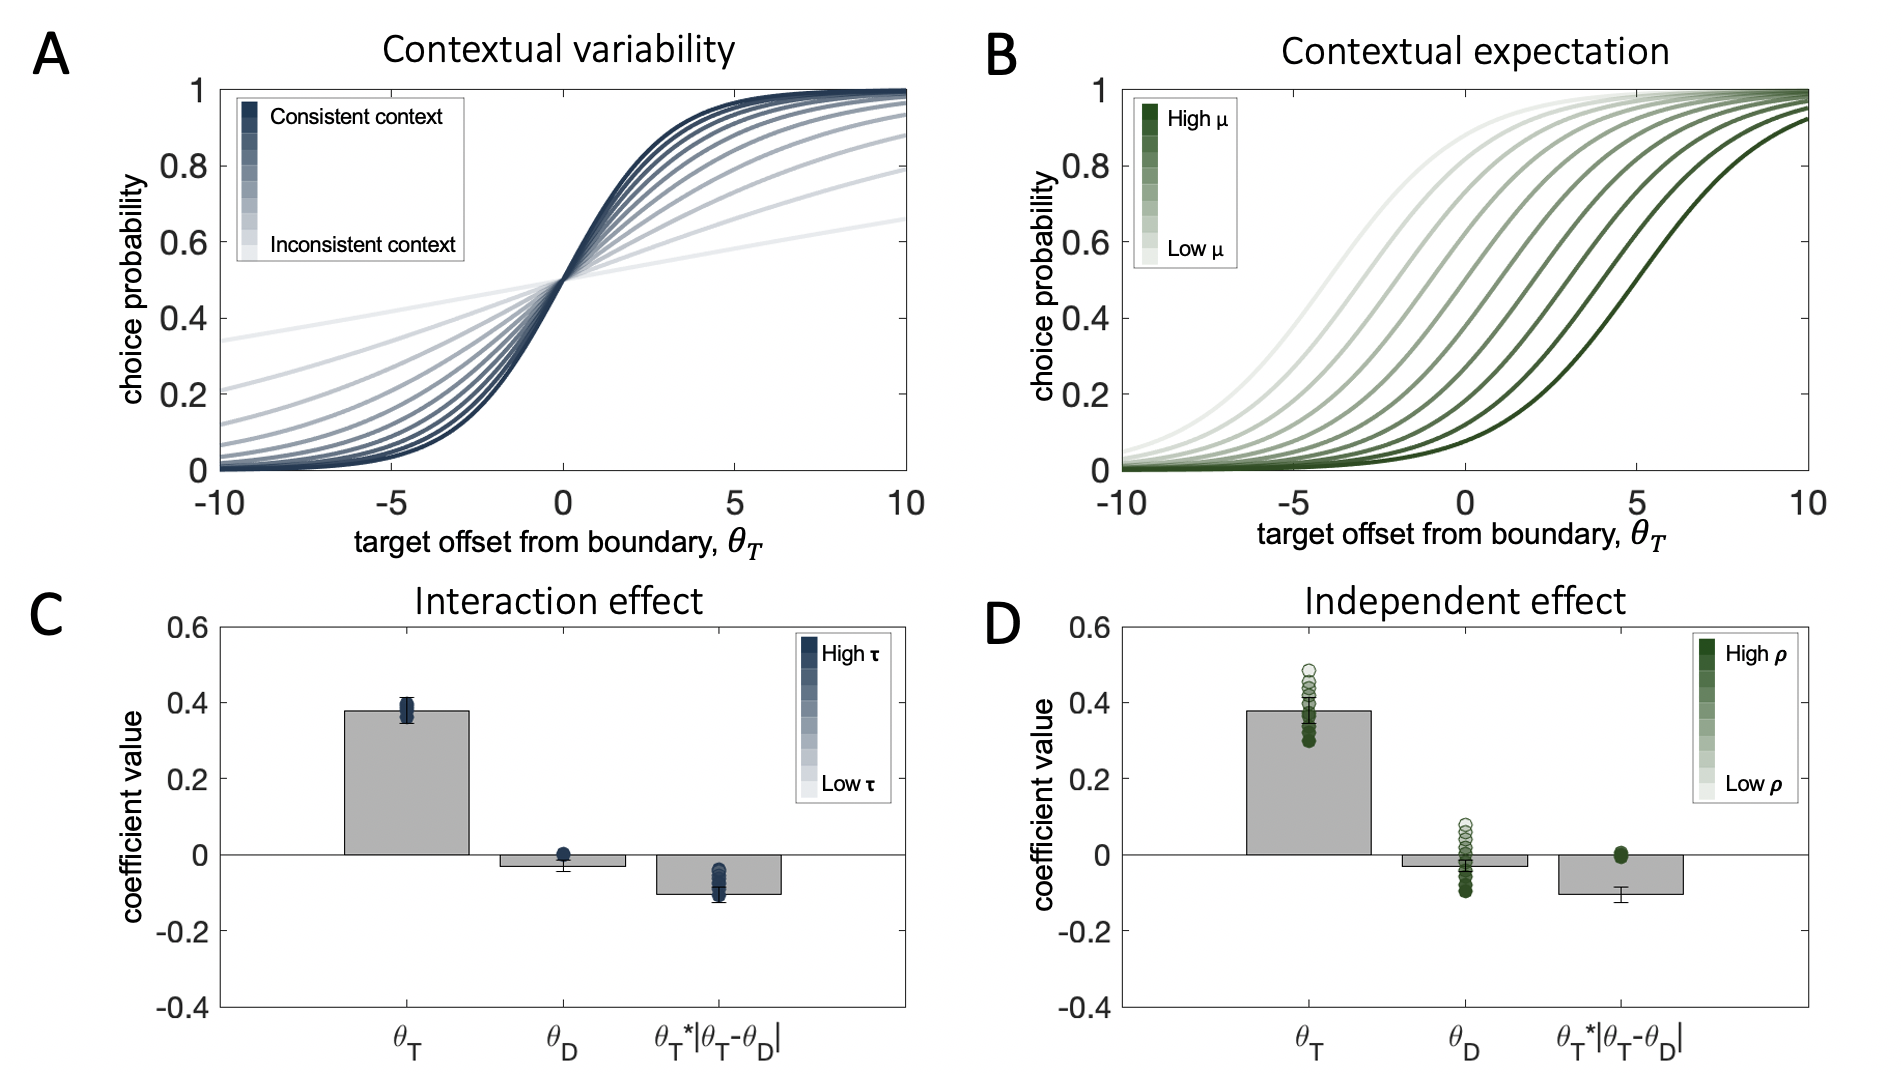
\includegraphics[width=1\linewidth]{figures/distr-model} 

}

\caption[Computational model, Simulations]{Model simulations of the effects of context on the transducer function translating decision inputs into choice probabilities (top) and on the distractor effects in choice behavior (bottom). $\textbf{A:}$ The consistency of context changes the slope of the transducer. Lower contextual variability leads to steeper slope (darker blue curves) and vice versa for high variability (lighter blue curves). $\textbf{B:}$ The contextual expectation changes the location of the inflection point of the transducer. A high contextual average leads to a transducer shifted rightwards along the x-axis (darker green curves) and vice versa for low contextual average. $\textbf{C:}$ Contextual variability leads to an interaction effect of the distractor (target-distractor consistency). Bars correspond to coefficients from a regression on human choices from Experiment 1, filled circles correspond to an analogous regression on model simulations where we varied parametrically the value of $\tau$, while keeping $\rho$ and $r$ constant. The higher the value of the multiplicative free parameter $\tau$, the stronger the consistency effect (darker circles). $\textbf{D:}$ The contextual expectation leads to an independent effect of the distractor. Bars correspond to coefficients from a regression on human choices from Experiment 1, filled circles correspond to an analogous regression on model simulations where we varied parametrically the value of $\rho$, while keeping $\tau$ and $r$ constant. The higher the value of the multiplicative free parameter $\rho$, the stronger the repulsion from the distractor (darker circles). Note that manipulations to $\rho$ do not lead to an interaction effect (overlapping circles on last bar).}\label{fig:distr-model}
\end{figure}

Here, \(y\) is the decision variable (as in Eq. \eqref{eq:distr-y}). A stimulus \(x\) is additively/subtractively modulated by the contextual biasing term \(\mu\) (in the attention literature this is sometimes known as a contrast gain effect, especially where the task involves detection) and multiplicatively/divisively normalized by a context variability term \(\sigma\) (similar to a multiplicative response gain effect). The degree of each type of gain control is respectively modulated by \(\rho\) and \(\tau\), and \(r\) is a regularizer; these 3 parameters are free to vary. Mapping this framework onto our experiment, the target feature \(x=\theta_T\), the context mean \(\mu=\frac{\theta_T+\theta_D}{2}\) and the context variability \(\sigma=|\theta_T-\theta_D|\), i.e.~it is given by the range of the two targets. We chose this measure of contextual dispersion over the more commonly used standard deviation, as our experimental manipulation comprised only two stimuli (target and distractor).

This compact formulation of the model allows us to visualize how changes to context affect the (sigmoidal) transducer function linking decision inputs to choice (see Eq. \eqref{eq:distr-y}). Changes in contextual variability adjust the slope of the transducer -- the more consistent the target and distractor, the steeper the slope (Fig. \ref{fig:distr-model}a), and consequently, the higher the gain of processing (Fig. \ref{fig:distr-model}c). The parameter \(\tau\) controls the degree of this change. As Fig. \ref{fig:distr-model}c shows, as \(\tau\) grows, the interaction effect of the distractor (target-distractor consistency) increases. By contrast, the contextual expectation shifts the transducer function along the abscissa (Fig. \ref{fig:distr-model}b). This impact translates into an independent effect of the distractor -- for negative values of \(\rho\) we observe an attraction towards the distractor, and for positive values of \(\rho\) we observe a repulsion (Fig. \ref{fig:distr-model}d). This rich pattern of distractor influence maps onto the variability of the independent effect observed in human participants across the three experiments (the coefficient estimates for \(\beta_2\) in Eq. \eqref{eq:reg-stepwise}).

\begin{figure}

{\centering 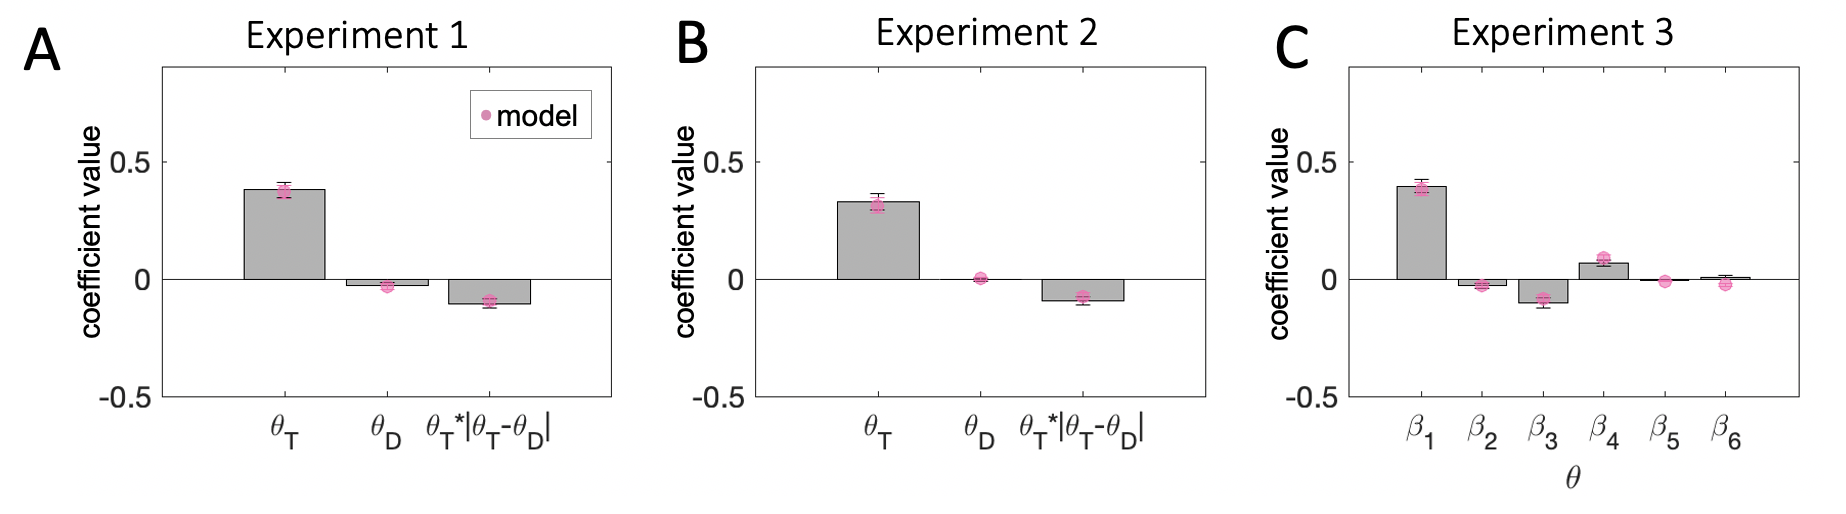
\includegraphics[width=1\linewidth]{figures/distr-model-fit} 

}

\caption[Computational model, Fits to human data]{Model fits to human data. $\textbf{A:}$ Experiment 1. $\textbf{B:}$ Experiment 2. $\textbf{C:}$ Experiment 3. Across all three experiments bars correspond to coefficients from a regression on human choices and pink circles correspond to model-simulated choices with free parameters estimated to best fit human data. Error bars correspond to standard errors of the mean. Coefficient labels in Experiment 3 are as in the regression analysis plot.}\label{fig:distr-model-fit}
\end{figure}

We fit this 3-parameter normalization model (\(r\), \(\tau\), and \(\rho\)) to human data from the first two experiments through gradient descent at the single trial level. Best fitting parameters were estimated for each participant individually by minimizing negative log likelihood. The model captures the pattern observed in the human data remarkably well (Fig. \ref{fig:distr-model-fit}a-b). It recreates both the independent and interaction effect of the distractor. It is also quantitatively favored over a static model (where \(\tau=\rho=0\)) by Bayesian model selection on cross-validated model likelihoods (exceedance probabilities: Exp.1: \(p=0.99\), Exp.2: \(p=0.99\)).

To account for the observed effect of attention in Experiment 3, we allowed the parameter \(r\), which captures the baseline slope of the transducer above and beyond the impacts of contextual consistency, to vary freely across cueing conditions. Thus, in our process model, the spatial attention manipulation does not affect the strength of contextual normalization indexed by parameters \(\tau\) and \(\rho\). Rather, it changes the overall sensitivity to the target, as evidenced by the estimated parameter values: the slope of the transducer was steepest (i.e.~lowest value for parameter \(r\)) in valid trials and shallowest (i.e.~highest value for parameter \(r\)) in invalid trials (valid \textless{} invalid: \(t_{19}=3.94\), \(p<0.001\), valid \textless{} neutral: \(t_{19}=3.79\), \(p=0.001\), neutral \textless{} invalid: \(t_{19}=2.46\), \(p=0.02\)). Indeed, incorporating attention in this manner in the normalization model reproduced the observed changes in sensitivity to target orientation (Fig. \ref{fig:distr-model-fit}c - \(\beta_4\)). Moreover, it captured the attention-independent effects of the distractor (\(\beta_2\) and \(\beta_3\)), as well as the lack of interaction of those with cueing condition (\(\beta_5\) and \(\beta_6\)).

\hypertarget{discussion-1}{%
\section{Discussion}\label{discussion-1}}

Across all three experiments, we found consistent evidence that distractors mainly influence choices by modulating the influence that targets have on choices. Our experiment involved a classic perceptual task -- discrimination of noisy gratings -- and our stimuli were spatially separated across the two hemifields, minimizing retinotopic visual interactions in the sensory encoding of target and distractor. Yet, our modelling suggests that targets have a stronger effect on choices when they are similar to distractors. This result was consistent using both conventional regression-based modeling and an approach based on reverse correlation analysis across all three experiments. This finding does not necessarily contradict, but does potentially nuance, previous accounts of distraction. For example, a standard model assumes that targets and distractors compete independently to influence choice, with the job of control processes being to upweigh targets at the expense of distractors.

In a different study, which is notable for applying a very rigorous modelling approach to a large body of data gathered from tasks that broadly resemble our own, the authors \autocite{shen2019} characterize the effect of distractor as being a generalized decrement to precision, or an increase in overall lapses of judgment (i.e.~guess rate). However, their analysis does not attempt to ask how the features of target and distractor impact choices, but rather compares experimental conditions that have different levels of distraction, which might have led to their overlooking any interaction between target and distractor that is present in that data.

Relatedly, this finding is not consistent with a familiar framework for understanding decisions based on multiple, potentially noisy, sources of information with variable decision-relevance -- that which is formalized by Bayesian inference \autocite{dayan1999,eckstein2009}. In our experiment, a Bayesian ideal observer would weigh the target and distractor according to how relevant they were judged to be for the decision. How this relevance was determined would have to depend on some assumptions about the likely sources of error in the task, but in general, this class of explanation would point to decisions being determined exclusively by a weighted mixture of independent target and distractor features. This is not what we observed.

The form of the interactive effect we did observe seems related to a phenomenon has been previously described as a consistency bias \autocite{cheadle2014}. A consistency bias occurs when stimuli that resemble the local context are processed with heightened gain, and so have greater impact on choices. Previous work has reported a bias for decisions to be consistent with the recent temporal context, which is captured by a normalization model analogous to the one we discuss here \autocite{cheadle2014}. A closely related paper showed that a range of phenomena relating to spatial context -- from across the subfields of perceptual, cognitive and economic decision-making -- can be explained with a gain control model that also resembles the one described here \autocite{li2018}. Thus, seemingly unrelated phenomena such as the tilt illusion \autocite{blakemore1970}, congruency effects in a Flanker task \autocite{eriksen1974} and the distracting effect of decoy food items \autocite{louie2013} can all be captured by a closely related interactive model in which items that are similar to the context are processed with higher gain.

We observed an interaction between target and distractor decision values (tilt relative to the boundary) rather than perceptual values (raw tilt). This implies that the distractor, as well as the target, is placed in a frame of reference that expresses tilt relative to the category boundary. Consistent with this finding, a previous study using EEG found evidence from neural encoding that both target and distracting signals are placed in a decision-based frame of reference \autocite{wyart2015}, although of course it is likely that the extent to which selection occurs early or late depends on both the nature of the task and the available resources \autocite{lavie1994}. The data described here suggest that the interaction between target and distractor occurs at this later stage, beyond immediate sensory perception. This perhaps surprising result is in line with previous reports on the consistency bias \autocite{cheadle2014} which also found that this effect occurred at a later stage of processing by dissociating sensory and decision inputs (via asking participants to make a decision based on the cardinality or diagonality of grating orientations). The finding that the contextual influence of perceptual distractors operates on decision level signals could perhaps also be anticipated from the many reports of contextual effects for stimuli that share an abstract property (such as value) but not a low level property (such as tilt), for example, in the literature on decoy effects discussed in the previous chapter.

We found limited evidence that the distractor impacted choices directly. The independent effect of the distractor appeared to largely vary idiosyncratically between participants both in terms of strength and direction. On the group level, this independent effect seemed to be reliable in Experiment 3, but was weaker in Experiment 1. Of note, these are the tasks for which the category boundary is the same for target and distractor, so it seems likely that any such effect (unlike the contextual consistency bias) operates at a perceptual, not a decision level. It is notable that the direction of the effect is repulsive, meaning that the more clockwise the distractor is, the less likely participants are to respond ``clockwise''. The observed repulsion of choices from the sensory features of the distractor across Experiments 1 and 3 is also consistent with the weak independent effect we found in Experiment 2 (see section \ref{interim-discussion-2}).

Indeed, contextual effects in sensory processing, such as adaptation over time \autocite{webster2015} and the tilt illusion \autocite{blakemore1970}, typically follow a repulsive pattern. The tilt illusion features grating stimuli similar to the ones we use here, however, the distracting flankers are closer to the target compared to in our set up. The higher degree of spatial separation can account for the weak and inconsistent nature of the sensory level effects we observe. Similar spatial interactions are documented in contrast perception \autocite{chubb1989,xing2001}, where a central texture appears of lower contrast when surrounded by a high context texture compared to when surrounded by a uniform background. These psychophysical effects have previously been modeled in a normalization framework \autocite{carandini2012}. Here, we also demonstrate that the observed repulsive effect of the distractor can be captured by a model in which decision inputs are normalized by the contextual expectation. The direction of this effect cannot, however, be explained by a model in which target and distractor compete for attention and/or processing resources.

Finally, our findings also speak to the large literature which has explored the effect of attention on decisions made about a target stimulus in the face of distraction. In Experiment 3, we included a cueing manipulation that allowed us to test how attention might be deployed to mitigate the effect of distraction. Although we saw that spatial attention enhanced target processing -- as demonstrated by both conventional and reverse correlation approaches -- it did not seem to have any impact on the consistency bias. In other words, both target and distractor were elaborated into the frame of reference of the decision (Experiment 2) and then apparently interacted in a way that drove choices, but at no point (as far as we can see) did spatial attention intervene to facilitate or inhibit this process (Experiment 3). This finding seems hard to reconcile with physiological work with non-human primates, which shows that when spatial attention is directed towards a target stimulus, contextual modulation of neural responses by irrelevant stimuli in extra-striate area V4 is reduced by approximately 50\% \autocite{sundberg2009}. This discrepancy might be related to the fact that the consistency bias appears to operate on the decision level rather than on the raw sensory signals likely captured by electrophysiological work in visual areas. In our data, spatial attention appeared to multiplicatively increase the gain with which a target stimulus is encoded \autocite{carandini2012}, but it did not modulate the independent or contextual effect of the distractor.

This pattern of results parallels findings on feature-based attention, which is known to operate broadly and independently of spatial attention \autocite{liu2007}, and which has been associated with a feature-similarity gain control process not dissimilar from the consistency bias reported here. For example, when attention is cued towards a visual feature -- such as downwards motion -- in one part of the visual field, neurons sensitive to downwards visual motion (but with receptive fields at different locations) show heightened responses \autocite{treue1999}. In attention studies, feature gain similarity also affects performance, albeit as potentially nonmonotonic function of target-distractor feature disparity \autocite{stormer2014,liu2019}. However, in our study there was no overt cueing of features. One possibility is that there is an automatic feature-similarity gain process that depends on the context provided by the distractor. Future work can shed light on the relationship between the phenomena reported here, and the established literature on feature-based attention.

\hypertarget{conclusion-1}{%
\section{Conclusion}\label{conclusion-1}}

Perceptual decisions often occur in the presence of irrelevant information. Studies on attention have contributed greatly to our understanding of the behavioral signatures and neural underpinnings of focusing attention onto a target stimulus and away from irrelevant distractors. However, we know remarkably little about the influence distractors wield on choice. This chapter examined the functional relationship between the features of a distractor stimulus and perceptual decisions. Across three experiments, we found consistent evidence that distractors affect perceptual decisions primarily through an interactive effect, whereby consistency between target and distractor features boosts sensitivity to the target. This effect appears to operate on the level of the decision, rather than on raw sensory inputs, and is independent of attention. A simple normalization framework, where the dispersion of features present in the local context determines the gain of processing of decision-relevant information, can capture the behavioral signatures of distraction in our results, across all three experiments.

\hypertarget{acknowledgements-1}{%
\section{Acknowledgements}\label{acknowledgements-1}}

This chapter is submitted for publication and available as a preprint \emph{Dumbalska, T., Rudzka, K., Smithson, H. E., \& Summerfield, C. (2021). How do (perceptual) distractors distract?.}

Experiment 3 formed part of Katarzyna Rudzka's final year undergraduate research project. Data collection for this experiment was carried out in its entirety by Katarzyna Rudzka. I am grateful for constructive feedback on an early draft of this chapter from my transfer of status assessors, Prof Jill O'Reilly and Dr MaryAnn Noonan. I also thank Prof Marisa Carrasco, members of her research group, and the participants in the Symposium on Biology of Decision Making (2019) for comments on presentations of this work.

\hypertarget{cat}{%
\chapter{Context-dependent categorization}\label{cat}}

\minitoc

\noindent 
\emph{Categorization decisions are repelled away from the characteristics of temporal context. This pattern of results is consistent across the realm of perception, cognition and economics; yet the underlying computational mechanisms that produce it remain elusive. This chapter arbitrates between putative sources of contextual bias in categorization decisions based on the lightness, size or numerosity of visual stimuli, across two experiments. Our experimental design allowed us to rule out response bias as a driver of the effect. We considered two alternative explanations: contextual shifts in the category boundary (contraction bias) and contextual changes in our encoding and experience of the current stimulus (adaptation). We used changes in suprathreshold sensitivity to estimate the contribution of adaptation. Our results suggest that adaptive changes to the appearance of the to-be-categorized stimulus can account for up to half of the contextual bias in lightness categorization, and for \textasciitilde10\% and \textasciitilde30\% of the contextual bias in categorizations of stimulus size and numerosity.}

\hypertarget{introduction-3}{%
\section{Introduction}\label{introduction-3}}

Sensory information is continuous, yet the choices we make based on it are necessarily discrete. In daily life, we seamlessly sort sensations into meaningful categories to guide our actions and behaviors. We do this by drawing boundaries through sensory space that divide the continuum of our experiences into distinct classifications. The location of those boundaries, however, is not static. It shifts over the course of our lifetime, starting with early cognitive development \autocite{gopnik1987,slawinski1998}, through our lived experiences \autocite{pollak2002} and domain-specific expertise \autocite{chi1981,shafto2003}. As we learn about the world, or a particular corner or field within it, our standards about what constitutes a particular category evolve, perhaps becoming more fine-tuned and consistent \autocite{slawinski1998,shafto2003}.

Interestingly, category boundaries may also shift on a much finer time-scale, depending on our most recent experiences. In the domain of visual perception, for instance, the same square stimulus can be categorized as small or large depending on the size of the squares that precede it (Fig. \ref{fig:cat-intro}a). If it happens to occur after several large squares, it would, on average, be more often categorized as small than if it happens to occur after several small squares. In the laboratory, this phenomenon has been examined by asking participants to categorize (or label) series of visual stimuli, presented one after the other. The experimenter would manipulate the distribution of stimulus characteristics: in some blocks, the participant may be presented with predominantly large stimuli; in others, they may be presented with predominantly small stimuli. The location of the category boundary in each experimental condition can then be quantified based on participant responses by estimating what stimulus size would lead to an equal proportion of ``large'' and ``small'' categorizations (known as the threshold or point of subjective equivalence/indifference point). The results of these experiments indicate the dynamic malleability of our categorization decisions. The location of the category boundary shifts predictably, tracking the central tendency of the distribution of stimulus characteristics present in the temporal context.

\begin{figure}

{\centering 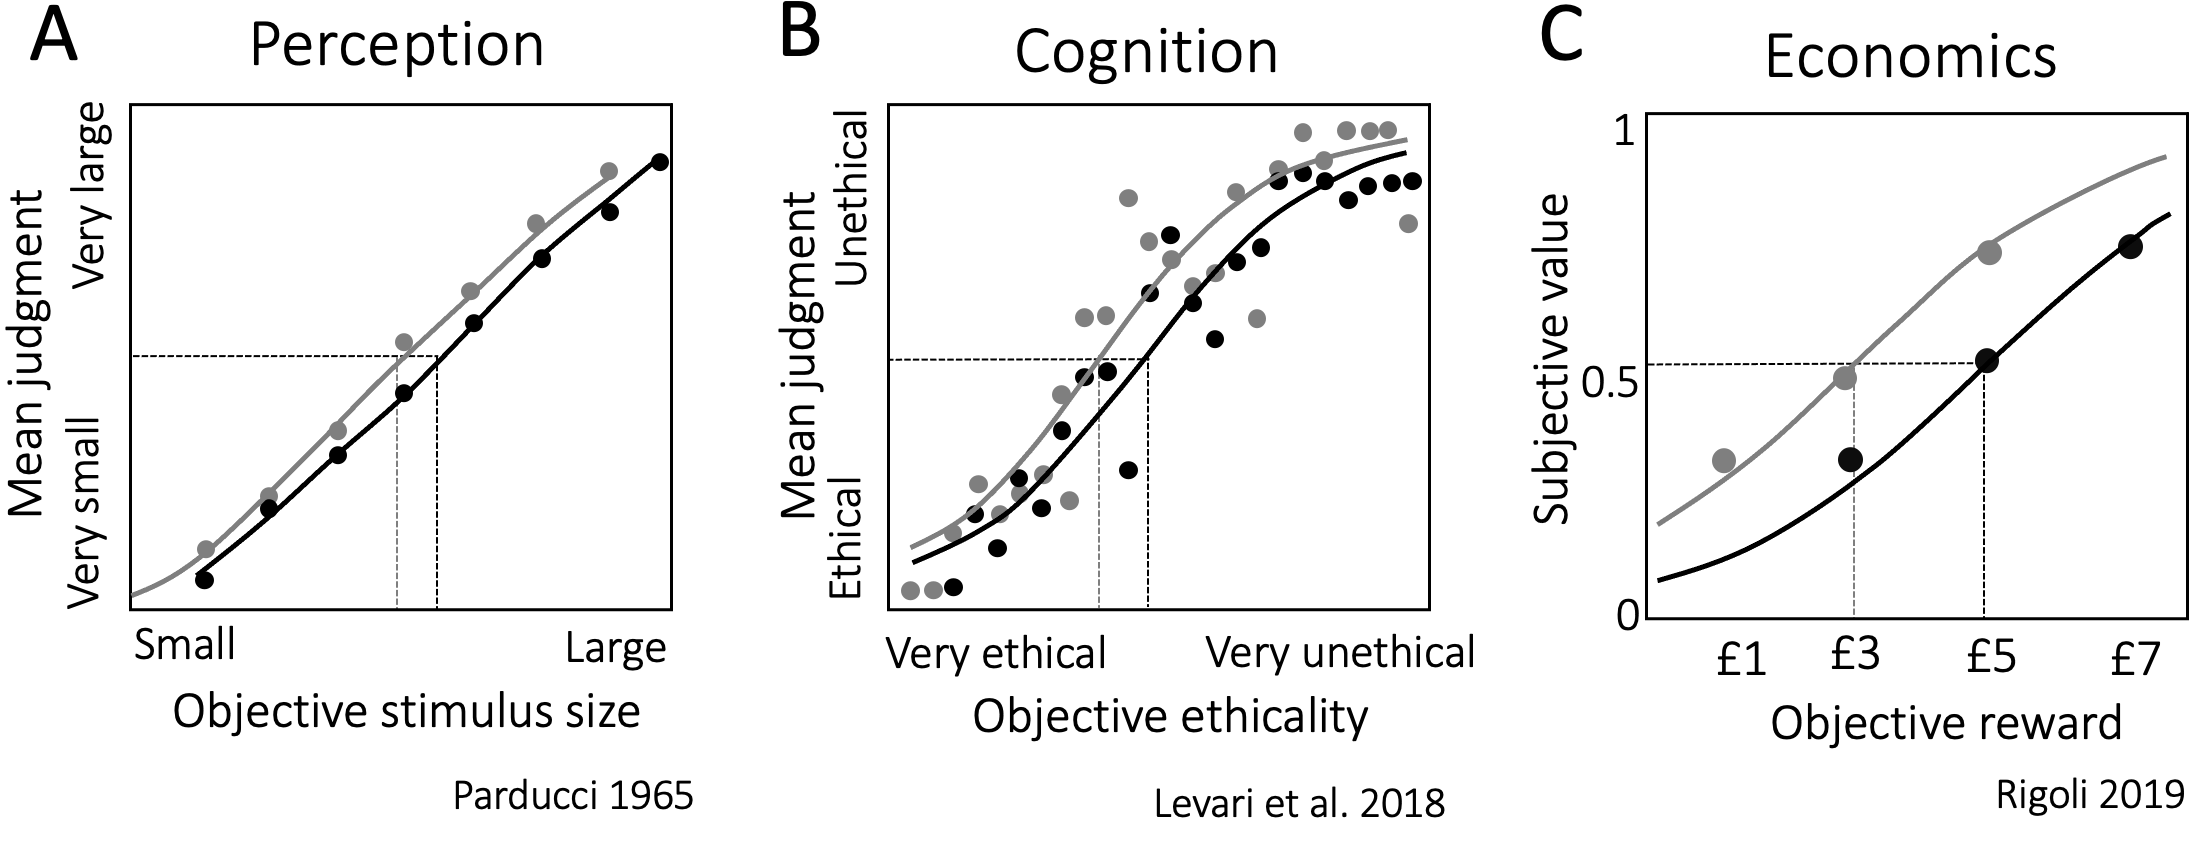
\includegraphics[width=1\linewidth]{figures/cat-intro} 

}

\caption[Context-dependent categorization across domains]{Context-dependent categorization across domains. Across all panels, the x-axis indexes the objective stimulus property and the y-axis -- categorization decisions. $\textbf{A:}$ Perception. Participants were asked to rate square stimuli on a scale between very large and very small. The psychometric curves depict participants' categorization decisions across two contexts. The grey curve tracks judgments in a context dominated by objectively smaller stimuli, the black curve tracks judgments in a context dominated by objectively larger stimuli. Data from Parducci 1965, Fig. 7. $\textbf{B:}$ Cognition. Participants were asked to accept or reject proposals for scientific studies that varied on a continuum of very ethical to very unethical (according to an independent group of raters). The shading of the curve again tracks context (grey: low prevalence of unethical studies, black: high prevalence of unethical studies). Data from Levari et al. 2018, Fig. 3b. $\textbf{C:}$ Economics. The psychometric functions here depict participants' subjective values estimated from choice behavior. Shading again tracks context (grey: low value context, black: high value context). Data from Rigoli 2019, Fig. 3a.}\label{fig:cat-intro}
\end{figure}

This pattern of results is robust. It generalizes across tasks that feature different types of visual stimuli \autocites[e.g.~spatial frequency,][]{lages1998}[distance,][]{morgan2000}[hue,][]{olkkonen2014}[facial expression,][]{levari2018} or engage other sensory modalities \autocites[e.g.~weight perception,][]{helson1947}[interval timing,][]{jazayeri2010}. It holds regardless of whether participants are asked to use their ``internal concept'' of the category \autocite{levari2018}, whether they are provided with an explicit or implicit standard for categorization, or with feedback on the accuracy of their judgments \autocite{morgan2000}. It also extends beyond perception, when we need to abstract away from sensory information to evaluate, for instance, scenarios based on their ethicality \autocite[Fig. \ref{fig:cat-intro}b,][]{levari2018} or economic prospects based on their subjective value \autocite[Fig. \ref{fig:cat-intro}c,][]{rigoli2019}. Temporal context sways judgments across perception, cognition and economics in a predictable fashion. Category boundaries track the frequency and dispersion of recently experienced stimulus properties \autocite{parducci1965,rigoli2019}, and so categorizations are repulsed away from recent experience. The smaller the squares we just saw, the more likely we would be to categorize a medium square as large. The more unethical the scenarios we just heard, the more likely we would be to judge an ambivalent scenario as ethical. The smaller the financial rewards we just experienced, the more likely we would be to perceive a moderate sum as valuable.

What drives this pattern of context dependence? One possibility is that it is driven by a response bias, whereby we calibrate our categorization judgments, such that the relative frequency of our actions remain stable across contexts. For instance, if we were faced with the choice of whether to accept or reject a proposal based on its ethicality, we might accept about half the proposals we encounter. But if the ethicality of proposals is particularly low in a given context (as it would be in the above described experimental manipulations) and we are compelled to accept half, this would naturally lead us to exhibit a lower threshold for (acceptable) ethicality. This is particularly likely in the laboratory, where response biases abound \autocite{poulton1989,bonnet1990}, as participants bring their priors (how likely is this category?), expectations of experiment demands \autocite[how would the experimenter like me to categorize this?,][]{rosenthal1976}, and misperceptions of randomness \autocite[can chance produce this sequence of categories?,][]{bar-hillel1991}. All of these factors may give rise to a response bias, producing the observed context-dependent behavior. It is difficult to rule out this possibility based on the empirical data, as the ground truth response frequency is necessarily confounded with the experimental manipulation of context. Response bias can, however, be minimized by careful experimental design; we took this route in the present study.

\begin{figure}

{\centering 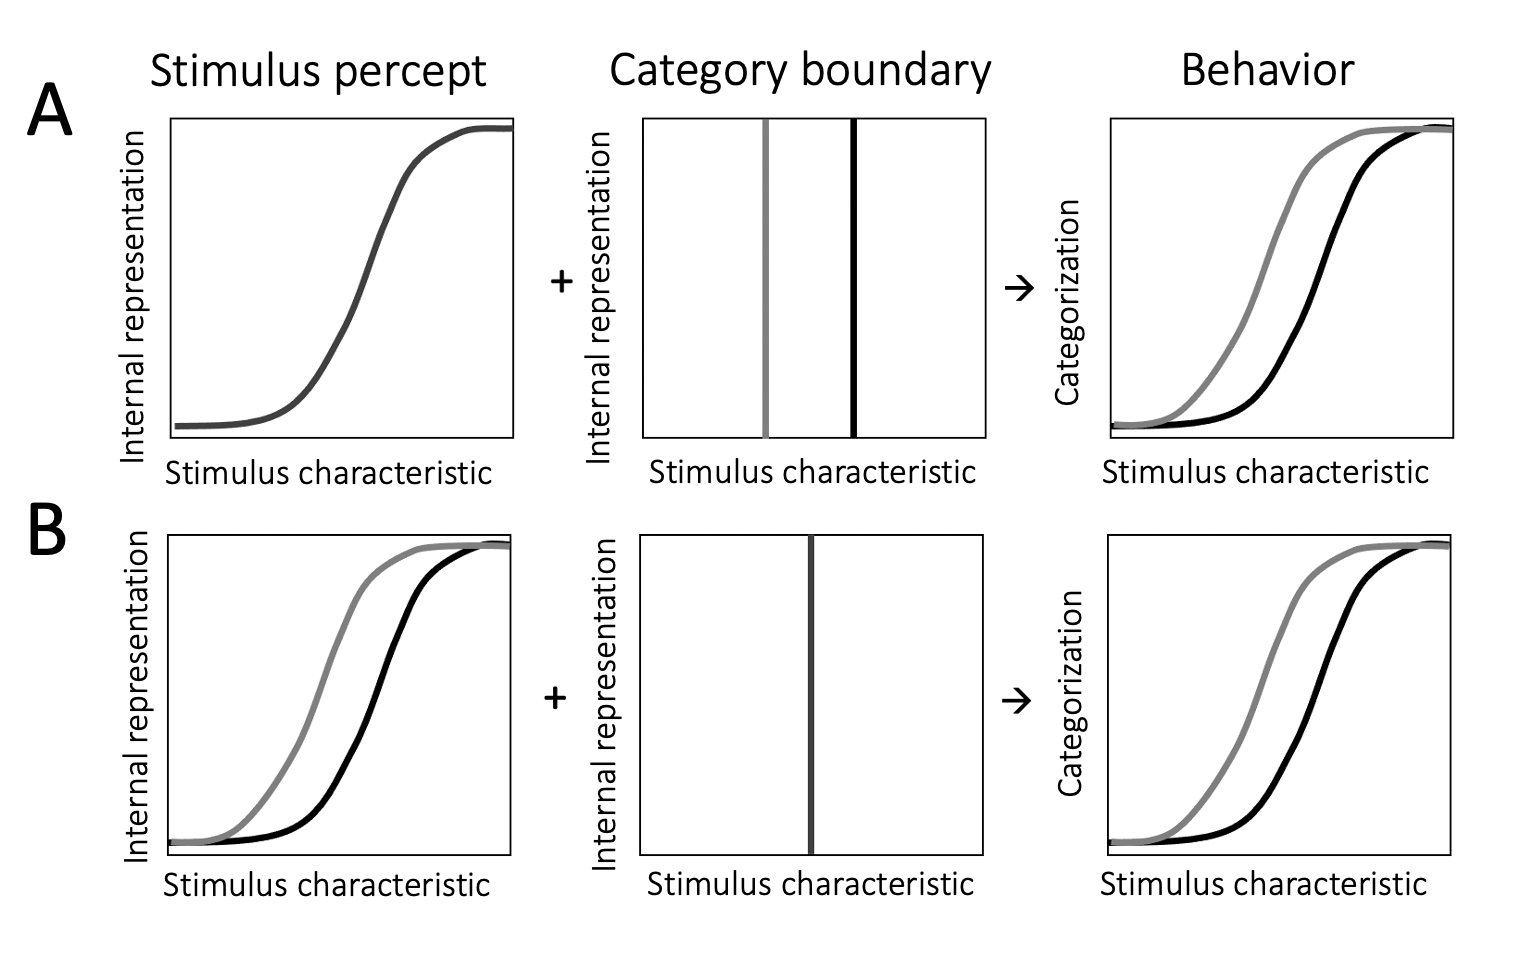
\includegraphics[width=0.8\linewidth]{figures/cat-expl} 

}

\caption[Sources of context dependence]{Possible sources of context dependence. $\textbf{A:}$ Participants' internal representation (left panel) of the stimulus is stable across contexts. Their representation of the category boundary (middle panel), however, changes such that it is lower in a context dominated by low stimulus property values (grey line) and higher in a context dominated by high stimulus property values (black line). This may be driven by a Bayesian process incorporating the prior distribution of stimulus characteristics in a noisy representation of the category boundary. It can lead to the observed context dependence in categorization decisions (right panel). $\textbf{B:}$ Participants' internal representation of stimulus property space shifts across contexts (left panel). This change may be driven by neural adaptation to contextual levels of stimulation. Participants' representation of the category boundary, however, remains stable (middle panel). This can also lead to the observed context dependence in categorization decisions (right panel). Note that both of these two processes can occur at the same time and influence categorizations together.}\label{fig:cat-expl}
\end{figure}

An alternative account, popular in the literature, argues that the internal representation of the standards we use to draw category boundaries is noisy. To make categorization judgments, we draw on a working memory reference for those standards. The precision of the reference, however, decays in memory \autocite{jou2004,ashourian2011,olkkonen2014a}. To resolve the uncertainty about its precise location in sensory (or conceptual) space, the neural system uses information available in the temporal context. It draws on the distribution of stimuli that have been recently experienced to form a prior; this prior then informs the standard. As a result, the category boundary differs across contexts -- it is biased towards the central tendency of context (contraction bias), and so, behaviorally, our categorizations exhibit the observed context dependence (schematic illustration in Fig. \ref{fig:cat-expl}a). A Bayesian account of this process, whereby the prior weighs more heavily in the presence of noise, is consistent with data showing that increasing the noisiness of the representation increases the contextual bias in categorizations. This can be done by, for instance, introducing cognitive demands \autocite{ashourian2011,allred2016} or manipulating delays between the reference and the to-be-categorized stimulus or the presentation quality of the reference \autocite{olkkonen2014}.

While this proposal puts the emphasis on our internal representation of the category boundary, context may also affect how we experience the current stimulus. Neural systems adapt to the levels of stimulation present in the environment. Visual adaptation to light, for instance, changes our sensitivity to stimulus brightness. After some minutes in darkness, we might be able to detect a faint light that would be indistinguishable to us in a bright room. These adaptive processes help calibrate the range of possible neural responses to the distribution of behaviorally relevant characteristics of the environment \autocite{webster2015} through normalization of each neural response by the pooled neural responses to context \autocite{carandini2012}. Adaptation can lead to changes in the appearance of stimuli, such that the neutral point (i.e.~the stimulus that would be considered neutral) is shifted towards the central tendency of context. For instance, adapting to a face exhibiting an angry facial expression, would alter how we perceive subsequent faces: objectively neutral faces will cease to feel neutral and objectively angry facial expressions will appear less angry and more neutral \autocite{webster2011}. This process may be illustrated as a recentering of the internal representation of sensory space towards the characteristics that dominate the temporal context (Fig. \ref{fig:cat-expl}b). This recentering would lead to the same stimulus being encoded and experienced differently depending on the temporal context in which it is encountered. Thus, even if the internal representation of the category boundary remains stable, adaptation can capture the observed context-dependent categorization behavior.

In addition to changes to the category boundary, normalization-based adaptive processes also bring about changes in sensitivity. The sigmoid shape of the transducer function, mapping sensory space onto an internal representation, is ubiquitous in neural systems; sensitivity is highest near the inflection point of the transducer. If the transducer shifts between contexts, tracking the distribution of features, then sensitivity would necessarily change too -- it would be highest for those stimulus characteristics that dominate the temporal context. Temporal context in adaptation, however, does not only encompass preceding task-relevant information. While the prior in a Bayesian process (as the one which might affect the location of the category boundary) is shaped by previously experienced instances of task-relevant stimuli, contextual influences on adaptation are less specific. Light adaptation, for instance, is driven by the overall light levels in the context, regardless of what light source is producing them (e.g.~light from a lamp + moonlight = overall level of light). By contrast, our prior for the brightness of moonlight would be driven by moon brightness on previous nights, and not by our previous experiences with lamplight.

In this chapter, we set out to examine the underlying mechanisms driving context-dependent categorizations across two experiments. First, we disentangled response frequencies from the frequencies of stimulus characteristics in our contextual manipulation to rule out response bias as a driver of context-dependent categorization (Experiment 1). Second, we used the specificity of contextual influences on categorizations (Experiment 1) and changes in sensitivity (Experiment 2), to probe whether and how much adaptation contributes to the observed context dependencies across categorizations based on sensory (Experiments 1 \& 2) and more abstract (Experiment 2) stimulus features.

\hypertarget{experiment-1-1}{%
\section{Experiment 1}\label{experiment-1-1}}

Experiment 1 measured the impact of temporal context on categorizations, controlling for biases in response frequencies introduced by the experimental manipulation. We did this by asking participants to complete one of two possible tasks on each trial. On some trials, participants had to categorize the lightness of a circle stimulus; on other trials, participants had to instead categorize its size. We manipulated the size context on trials asking about lightness categorizations only (and vice versa for lightness context manipulations). This ensured that participants were exposed to a biased set of stimulus sizes, but that they would not have to respond to disproportionately many objectively large stimuli in one context, and to disproportionately many objectively small stimuli in another. This eliminated the possibility that context-dependent categorizations could be driven by a bias, whereby participants might be striving for an equal number of ``large'' and ``small'' categorizations across contexts. At the same time, it also made it so that any such bias would act in opposition of the contextual effect. That is, in our design, responding ``large'' as equally often as ``small'' would lead to a stable categorization boundary across the different contexts, as size trials are composed of an equal number ``large'' and ``small'' ground truth categorizations in all contexts.

Experiment 1 also manipulated the timing of trials to examine two additional research questions. First, is the contextual bias in categorization decisions stronger when participants have had the opportunity to experience (and potentially, adapt to) each stimulus for longer? To address this question, we compared the contextual effect on category boundaries between a short (200ms) and long (1000ms) stimulus presentation condition. And second, how specific is the contextual effect? Is it just the context provided by task-relevant stimuli that impacts categorizations, or does the visual environment more generally also influence the location of the category boundary? The timing manipulation allowed us to examine this as participants' visual environment, and consequently exposure to task-irrelevant properties, differed between the two stimulus timing conditions.

\hypertarget{methods-6}{%
\subsection{Methods}\label{methods-6}}

\hypertarget{participants-4}{%
\subsubsection{Participants}\label{participants-4}}

Ten participants (aged 22.3 ±4.37) with normal or corrected-to-normal vision took part in Experiment 1. The study received ethical approval from the Central University Research Ethics Committee at the University of Oxford (approval reference number: R58531/RE001) and took part in the Perception Laboratory at the Department of Experimental Psychology. All participants provided written informed consent and were compensated with either course credit or £10 per hour for their time.

\hypertarget{apparatus-3}{%
\subsubsection{Apparatus}\label{apparatus-3}}

Participants were seated in a dark room approximately 175cm away from a computer monitor (1080x1080 resolution, 32' Display++ LCD monitor) with linearized output light intensities. Visual stimuli were created and presented with ViSaGe, CRS Toolbox (Cambridge Research Systems) for MATLAB.

\hypertarget{stimuli-3}{%
\subsubsection{Stimuli}\label{stimuli-3}}

Stimuli in the experiment consisted of grayscale circles presented on a light yellow background (CIE X=.372, Y=.400, Z=76.1\(cd/m^2\)). We followed previous work in lightness perception in choosing a chromatic background to minimize background-anchoring effects (e.g.~to the minimum lightness available -- black background, the maximum -- white background, mean -- half-contrast grey, etc.). For the contextual manipulation, we constructed 3 types of stimulus sets (low, neutral and high) for 2 stimulus property dimensions (lightness and size). For each of the two stimulus dimensions we first generated an array of 16 possible property values. Those values corresponded to the radius of the circle in pixels, and the lightness of the circle in 10-bit pixel values. We then sorted those values into two biased sets (low set: the lowest 10 values, high set: the highest 10 values) and a neutral set (the middle 10 values).

We constructed the full arrays of property values using a perceptual difference scale of lightness and size, which we estimated with a pilot group of participants (n=6, following same ethics protocol R58531/RE001) via maximum likelihood difference scaling \autocites[MLDS,][see Experiment 2 for details on this method]{maloney2003,knoblauch2008}. We took this approach to ensure that the stimuli we employed in the experiment would all be equally discriminable. The size array ranged from 90 to 210 pixels in steps of 8 pixels (corresponding to approximately \(1.09\)° to \(2.54\)° of visual angle at the viewing distance of the display). Note that linear step sizes in terms of radius are quadratic in terms of circle area. The lightness array ranged from 24 to 75\(cd/m^2\) in steps of 3.4\(cd/m^2\). The linear perceptual spacing of lightness we observed in piloting mirrors past results for this luminance range, \autocites[e.g.][]{wiebel2017,rogers2016}.

\hypertarget{experimental-procedure-3}{%
\subsubsection{Experimental Procedure}\label{experimental-procedure-3}}

Each participant completed the experiment in a single hour-long session. The experiment consisted of 2 practice blocks and 30 test blocks of 60 trials each. Each block started with an example circle stimulus whose lightness and size corresponded to the median of the overall stimulus set. Participants were advised that they could use this circle as a reference for neutral (or medium) size and lightness.

The first practice block served to familiarize participants with the experiment. Stimuli were presented for up to 4 seconds, until a categorization response was registered. The block continued until the participant achieved an average response time of 1.5 seconds or below. The length of the first practice block was constrained to be of a minimum of 80 trials and a maximum of 150 trials. The second practice block comprised 100 trials and introduced a shorter stimulus duration -- 200ms.

\begin{figure}

{\centering 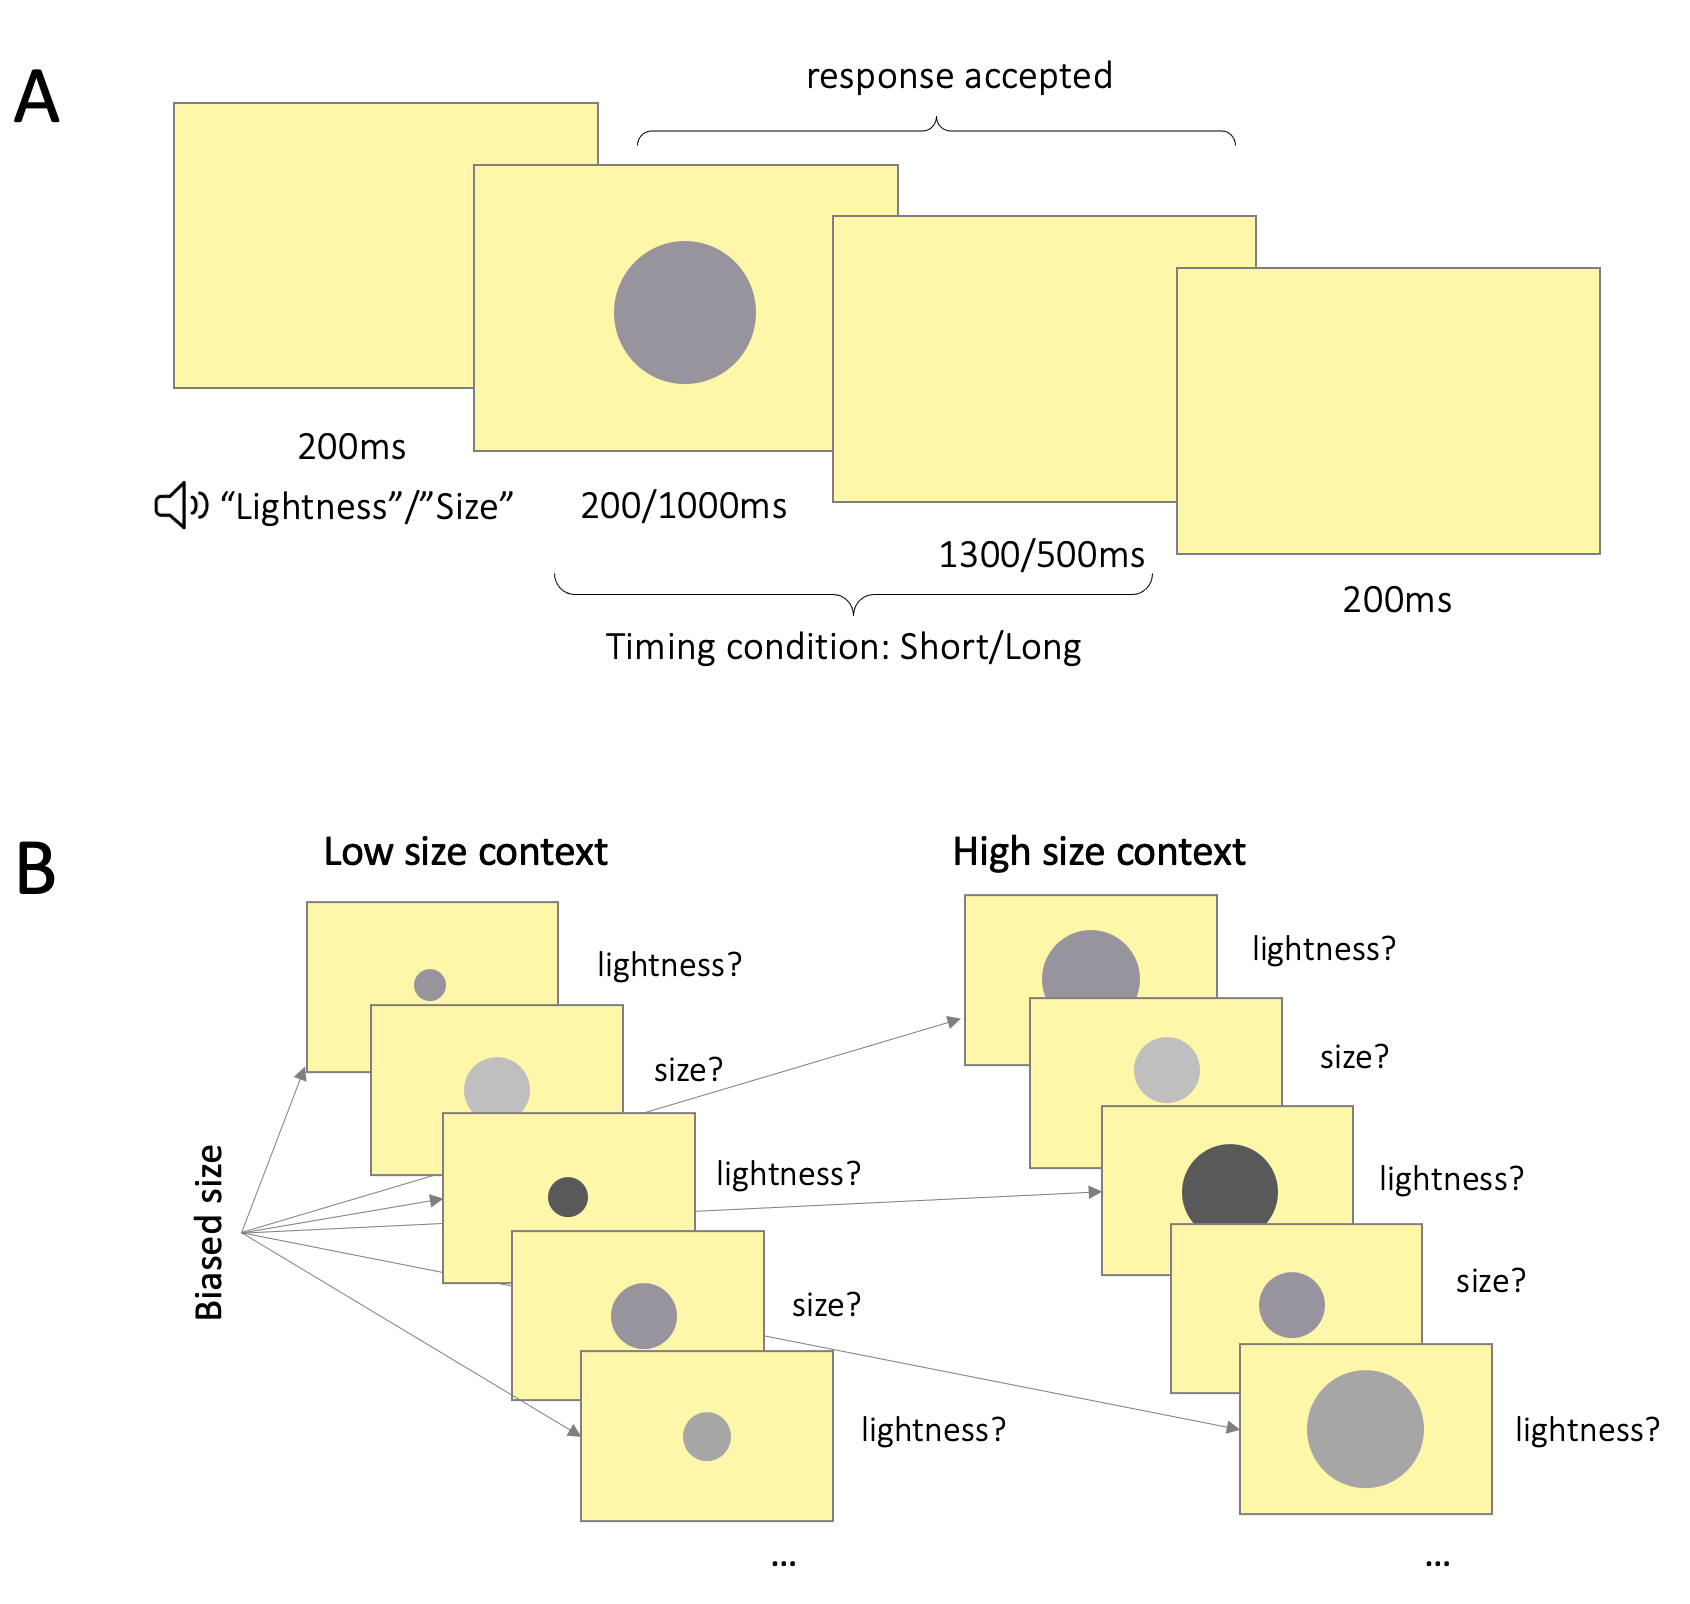
\includegraphics[width=1\linewidth]{figures/cat-trial-a} 

}

\caption[Experiment 1, Trial structure]{$\textbf{A:}$ Trial structure. Participants first heard a computer generated voice announce the trial type. 200ms following this, a circle stimulus was presented in the center of the screen for either 200ms or 1000ms. In size trials, participants had to categorize the stimulus as small or large; in lightness trials, as light or dark. Responses were accepted for 1.5s starting from stimulus onset. The stimulus remained on the screen for the full stimulus duration even if the participant responded prior to stimulus offset. There were 200ms breaks between trials. $\textbf{B:}$ Contextual manipulation. The left panel illustrates a sequence of 5 trials in a low size context, the right panel -- in a high size context. Across both panels, in trials asking about size, stimulus size was drawn from a neutral set, such that half the stimuli would be objectively small and half the stimuli -- objectively large. In trials asking about lightness, stimulus size was drawn from biased sets, such that stimulus size would on average be lower in the low context, and higher in the high context.}\label{fig:cat-trial-a}
\end{figure}

In each trial (Fig. \ref{fig:cat-trial-a}a), the participant first heard a computer-generated voice (Google Text-to-Speech API, gender neutral voice) announce the type of trial, by producing either the word ``lightness'' or ``size''. 200ms after the onset of the voice, a circle appeared on the screen. In size trials, participants had to categorize the circle as either large or small; in lightness trials, participants had to categorize the circle as either light or dark. Responses were accepted until the end of the trial, 1.5 seconds post stimulus onset. There was a 200ms interval between trials.

The experiment followed a 2x5 factor design. The first factor was timing -- in half of the blocks, stimuli were presented for 200ms (brief condition), and in the other half of the blocks -- for 1000ms (long condition). The timing manipulation allowed us to test whether the contextual effect is stronger when the participant has had the opportunity to adapt to the stimulus set for longer. That is, is there an interaction between stimulus duration and the contextual manipulation? The timing manipulation also allowed us to test another question -- how specific is the contextual effect? Are categorization decisions impacted only by the context provided by previous \emph{task-relevant stimuli}, or do other, task-irrelevant inputs also affect categorizations? In the brief condition, participants were exposed to the background for longer than in the long stimulus presentation condition. As the luminance of the background (76\(cd/m^2\)) was higher than that of the stimuli (24--75\(cd/m^2\)), in the brief condition, participants were exposed to a lighter visual environment compared to in the long condition. If participants' categorization decisions were influenced by the properties of the task-relevant stimuli only, lightness categorizations should not differ between the brief and long conditions (since the relative frequencies of stimulus lightness values are matched across the long and short conditions). But if the contextual effects were driven by a more general adaptive process which is not specific to the imperative stimuli, we would expect lightness categorizations to differ between the two timing conditions (with higher thresholds in the brief condition). For size, as participants were seated in a dark room, the only obvious size reference available in the gaps between stimulus presentations was the size of the screen itself. By contrast, during stimulus presentations, the size environment included both the size of the monitor and the (relatively smaller) size of the current stimulus. Thus, the size environment was on average smaller in the long condition (where stimuli were presented for longer) that in the brief condition. We reasoned that, according to the adaptation hypothesis, this might lead to the same pattern of contextual bias for size as for lightness -- higher categorization thresholds in the brief condition.

The second experimental factor was the contextual manipulation. In each block, we manipulated the context for only one stimulus dimension by using a biased set (i.e.~either the low or high stimulus set) in the trials that asked about the \emph{other} stimulus dimension (Fig. \ref{fig:cat-trial-a}b). For instance, in a ``high size'' block, stimulus size was drawn from the high size stimulus set only on trials that asked participants to categorize the lightness of the circle; on trials where the participant had to categorize the size of the circle, stimulus size was drawn from the neutral size stimulus set. This ensured that our contextual manipulation would not introduce a confounding response bias, i.e.~it would not skew the ground truth number of `large' responses. In each block, we manipulated the context for only one stimulus dimension, the context for the other stimulus dimension remained neutral (neutral stimulus set). This resulted in 4 combinations of context conditions (size-lightness: high-neutral, low-neutral, neutral-high, neutral-low), to which we added a fifth neutral condition (neutral-neutral).

Responses were registered via button presses on a hand-held number keyboard. Participants were instructed to hold the keyboard with both hands and respond with their left thumb on size trials, and right thumb on lightness trials (or vice versa, counterbalanced across participants). Categorizing a stimulus as ``large'' or ``light'' was associated with the press of an upper button; categorizing a stimulus as ``small'' or ``dark'' was associated with the press of a down button. As the timings of the trials were fixed, nothing changed on the screen upon participant response; instead, participants heard a click to confirm their choice was registered.

\hypertarget{analyses-4}{%
\subsubsection{Analyses}\label{analyses-4}}

First, we estimated psychometric functions separately for each participant and each condition in the experiment, using the Psignifit toolbox for MATLAB \autocite{schutt2015}. We tested whether the contextual manipulation biased participants' categorization decisions on the group level with a general linear model (GLM) of participant thresholds (normalized as a \(z\) score). The GLM quantified the impact of the contextual manipulation (coded as -1, 0, 1 for low, neutral and high), timing condition, and their interaction, controlling for the nonindependence of threshold measurements from the same observer. We followed up the results of the GLM with pairwise comparisons with paired samples \(t\) tests.

As a complementary approach for probing the effect of temporal context, we regressed participant choices on each trial on the relevant property of the stimulus on the current trial, as well as on the value of that same property on the previous 3 trials. Thus, for each participant we built two logistic regression models, one for lightness and one for size. In the model for size, the outcome variable comprised the responses to all trials asking the participant to categorize the size of the stimulus; the predictor variables included the size of the stimulus on the current trial \(t\), as well as the size of the stimuli on the immediately preceding 3 trials, \(t-1\), \(t-2\) and \(t-3\) (all predictors were \(z\)-scored). This approach allowed us to quantify the effect of stimulus history (size on previous trials, \(t-1\), \(t-2\) and \(t-3\)), controlling for the effect of the imperative stimulus (size on current trial, \(t-1\)). Note that as trial types (lightness or size categorizations) were interleaved, the predictor variables in the regression included both types of trials. For instance, in a regression on lightness categorizations, we included as predictors the lightness of stimuli on the preceding three trials; on some of those trials, the participant was likely asked to judge the size (and not lightness) of the stimulus. We assessed the statistical significance of the beta coefficients from the regression on the group level via one sample \(t\) tests.

\hypertarget{data-code-availability-statement-4}{%
\subsubsection{Data \& Code Availability Statement}\label{data-code-availability-statement-4}}

All data and code to reproduce the analyses are available in the OSF repository (\url{https://osf.io/vxh3n/}) for this project.

\hypertarget{results-6}{%
\subsection{Results}\label{results-6}}

\begin{figure}

{\centering 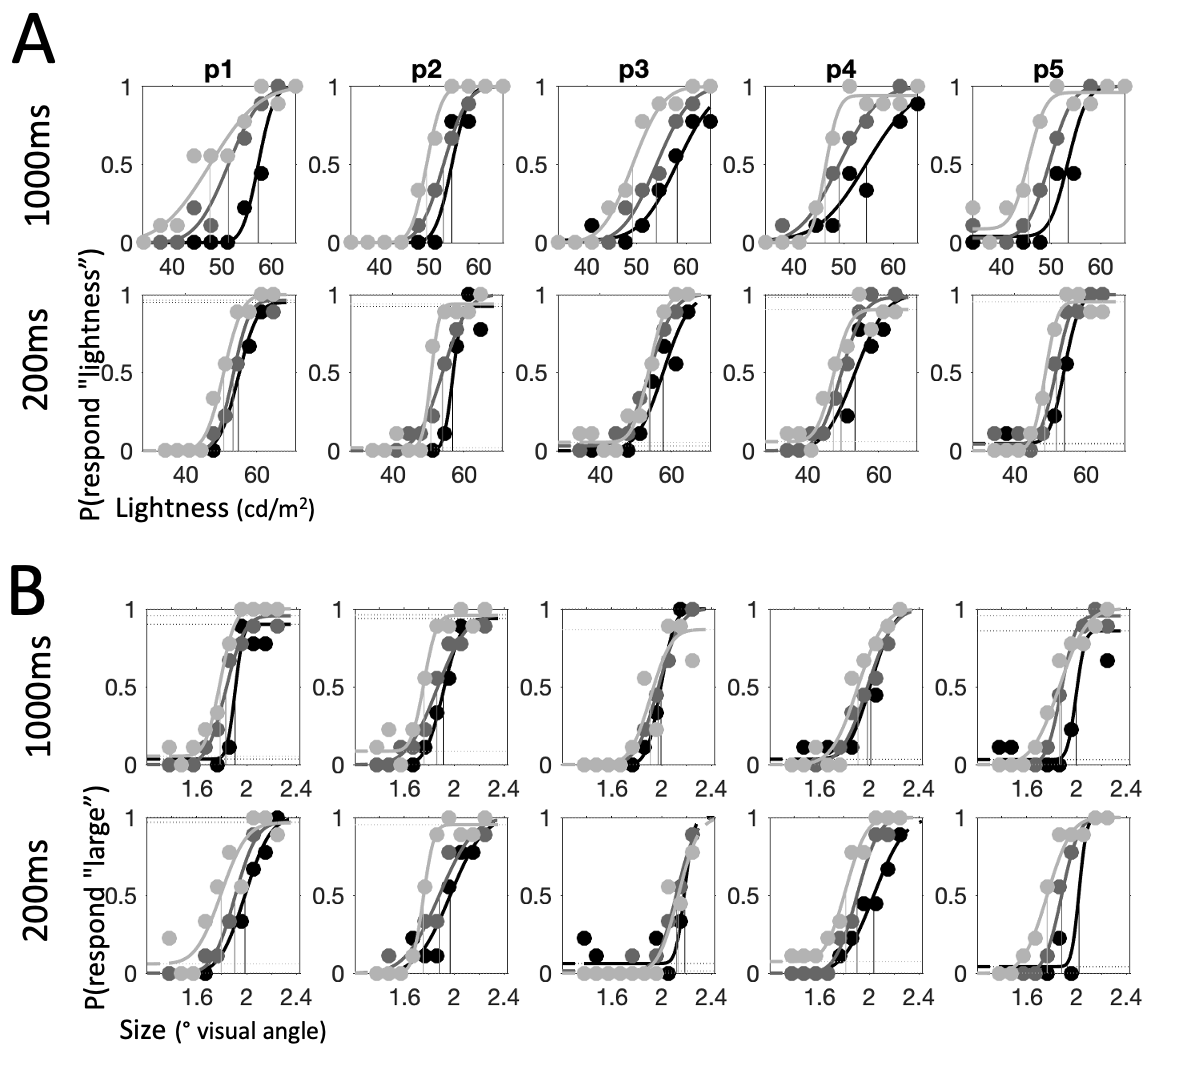
\includegraphics[width=0.9\linewidth]{figures/cat-psychom-ppt-a} 

}

\caption[Experiment 1, Psychometric functions, part 1]{Psychometric functions for each individual participant: first half of participants, continued in the next figure. Across all panels, columns depict individual participants (p1-p10). Shading tracks context (light grey: low, dark grey: neutral, black: high). Points show raw data, curves -- cumulative Gaussian functions fit to data. Vertical lines show threshold value estimates for each condition. $\textbf{A:}$ Psychometric functions for lightness trials. Top row shows long condition (1000ms) and bottom row -- short condition (200ms). $\textbf{B:}$ Psychometric functions for size trials. Top row shows long condition (1000ms) and bottom row -- short condition (200ms). }\label{fig:cat-psychom-ppt-a}
\end{figure}

\begin{figure}

{\centering 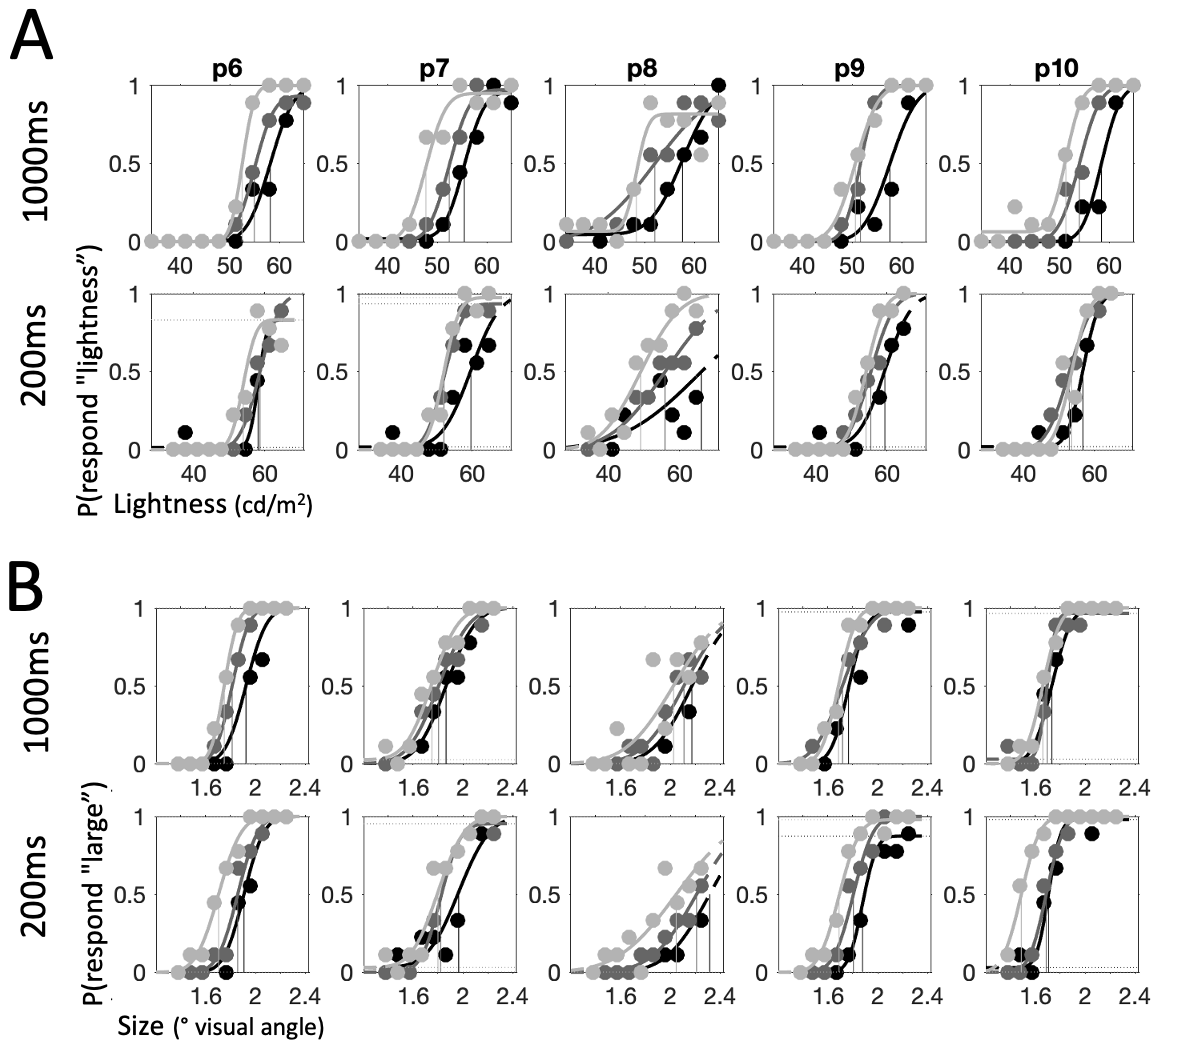
\includegraphics[width=0.9\linewidth]{figures/cat-psychom-ppt-b} 

}

\caption[Experiment 1, Psychometric functions, part 2]{Psychometric functions for each individual participant: second half of participants, continued from previous figure}\label{fig:cat-psychom-ppt-b}
\end{figure}

The psychometric functions for each participant are presented in Fig. \ref{fig:cat-psychom-ppt-a} and Fig. \ref{fig:cat-psychom-ppt-b} where each column represents one participant. While there is considerable variability in performance, there is also a clear pattern of dissociation of psychometric functions between the different context conditions. Generally, the psychometric function for the low condition (light grey) is shifted to the left and the psychometric function for the high condition (black) is shifted to the right relative to the psychometric function for the neutral condition (dark grey). These horizontal shifts in the psychometric function are captured by the parameter \(threshold\), which tracks the stimulus property value that corresponds to an equal probability of categorizing a stimulus as ``large'' or ``small'' (/``light'' or ``dark''). Threshold values are visualized in Fig. \ref{fig:cat-psychom-ppt-a} as vertical lines projecting downwards from the inflection point of each psychometric function.

The average values of the thresholds across participants are presented in Fig. \ref{fig:cat-psychom-a}. We quantitatively assessed the influence of context and stimulus timing on threshold values via a GLM, controlling for individual influences on thresholds. The contextual manipulation significantly influenced categorizations (lightness: \(\beta=0.81\), \(p<0.0001\), size: \(\beta=0.63\), \(p<0.0001\)), such that thresholds increased from low to neutral, and neutral to high conditions. Pairwise comparisons confirmed this pattern of results (lightness low\textless neutral: \(t_9=6.78\), \(p<0.001\), lightness neutral\textless high: \(t_9=8.66\), \(p<0.001\); size low\textless neutral: \(t_9=7.02\), \(p<0.001\), size neutral\textless high: \(t_9=7.97\), \(p<0.001\)).

Stimulus timing impacted lightness thresholds (\(\beta=-0.45\), \(p<0.001\)), with higher thresholds for lightness judgments in the brief presentation condition. Shorter stimulus timing also increased thresholds for size judgments (\(\beta=-0.21\), \(p=0.01\)), albeit the effect was weaker than for lightness. This pattern of results suggests that categorization decisions are subject to contextual influences going beyond the immediately task-relevant stimuli. In the brief condition, the relatively high lightness of the background provided a lighter visual environment across all context conditions, resulting in higher categorization thresholds for lightness. Similarly, the brief condition provided, on average, a larger size reference, leading to increased categorization thresholds for size. This result suggests that the visual environment (beyond the immediately task-relevant inputs) contributes to the contextual bias in categorization decisions.

\begin{figure}

{\centering 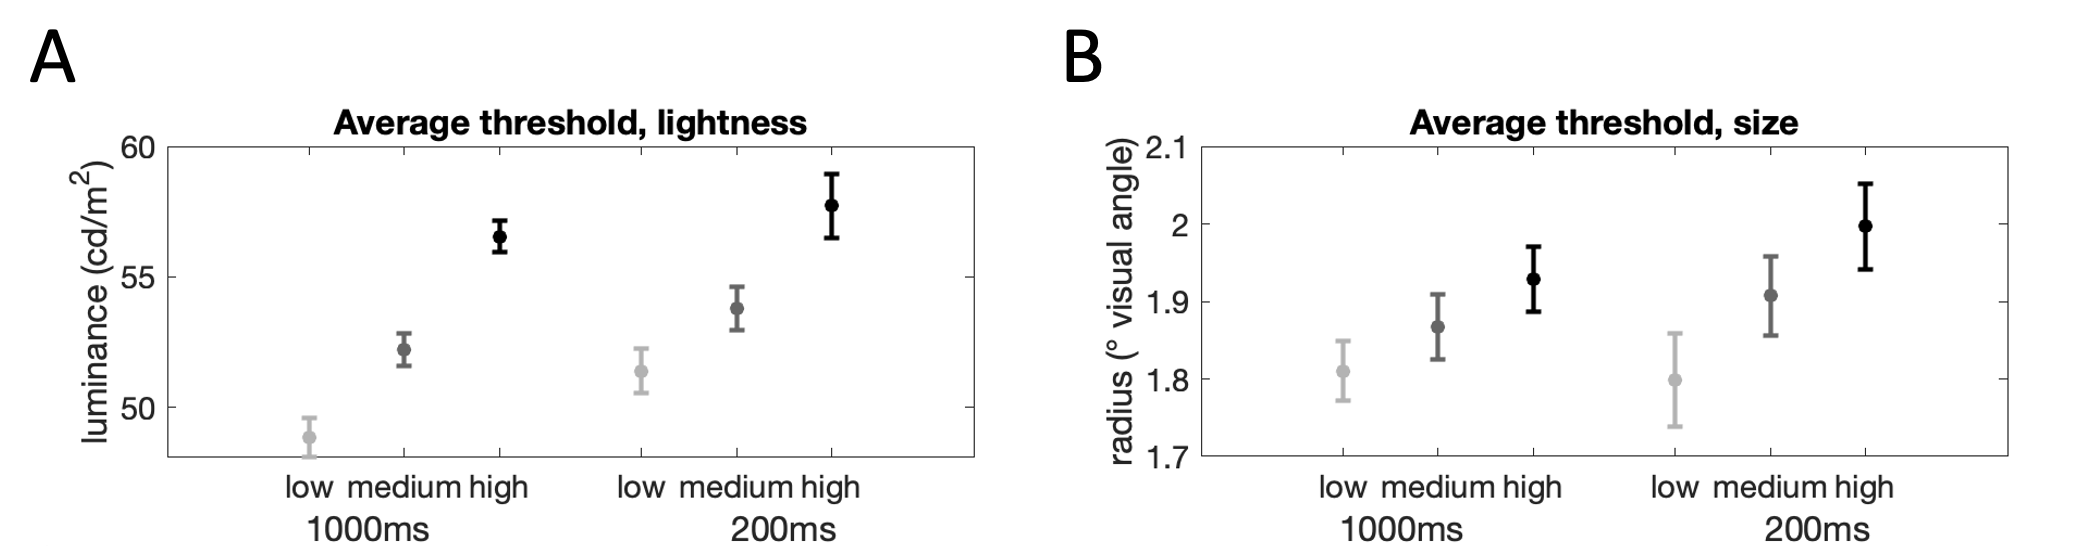
\includegraphics[width=1\linewidth]{figures/cat-psychom-a} 

}

\caption[Experiment 1, Threshold values]{Threshold values for each context condition (light grey: low, dark grey: neutral, black: high) and timing condition (left: long, right: short). $\textbf{A:}$ Lightness judgments. $\textbf{B:}$ Size judgments.}\label{fig:cat-psychom-a}
\end{figure}

Finally, the interaction between timing and context was not statistically significant for lightness (\(\beta=0.18\), \(p=0.20\)). This null result indicates that the contextual effect for lightness did not increase when participants were exposed to stimuli for longer (1000ms vs 200ms). The interaction between stimulus duration and context for size, however, was significant (\(\beta=-0.26\), \(p=0.01\)) indicating that the contextual effect \emph{decreased} when participants were exposed to stimuli for longer (1000ms vs 200ms). Note that this effect goes in the opposite direction of the adaptation prediction; an adaptive process should lead to stronger context-dependencies as stimulus duration increases.

We explored the effect of temporal context further by quantifying the influences of recent stimulus history on choice via a logistic regression. The resulting beta coefficients for the decision-relevant stimulus property on the most recent 4 trials are available in Fig. \ref{fig:cat-reg-a}. As expected, the lightness (\(t_9=14.31\), \(p<0.001\)) and size (\(t_9=14.95\), \(p<0.001\)) of the stimulus on the current trial were both strongly associated with a higher likelihood of categorizing it as light and large, respectively. Categorizations were, however, repulsed away from the properties of the stimulus on the preceding trials. Higher stimulus lightness on the previous trial(s) led to a lower likelihood of categorizing the stimulus on the current trial as light (trial \(t-1\): \(t_9=-5.00\), \(p<0.01\); trial \(t-2\): \(t_9=-10.10\), \(p<0.001\); trial \(t-3\): \(t_9=-7.24\), \(p<0.001\)). Similarly, higher stimulus size on the previous trial(s) led to a lower likelihood of categorizing the stimulus on the current trial as large (trial \(t-1\): \(t_9=-5.31\), \(p<0.001\); trial \(t-2\): \(t_9=-5.39\), \(p<0.001\); trial \(t-3\): \(t_9=-4.80\), \(p=0.001\)). Exploratory analyses (by adding more predictor variables to the logistic regression) indicated that the effect of stimulus history extended as far back as to the preceding 13 trials for lightness (trial \(t-13\): \(t_9=-3.17\), \(p=0.01\)), and the preceding 8 trials for size (trial \(t-9\): \(t_9=-4.13\), \(p<0.01\)).

\begin{figure}

{\centering 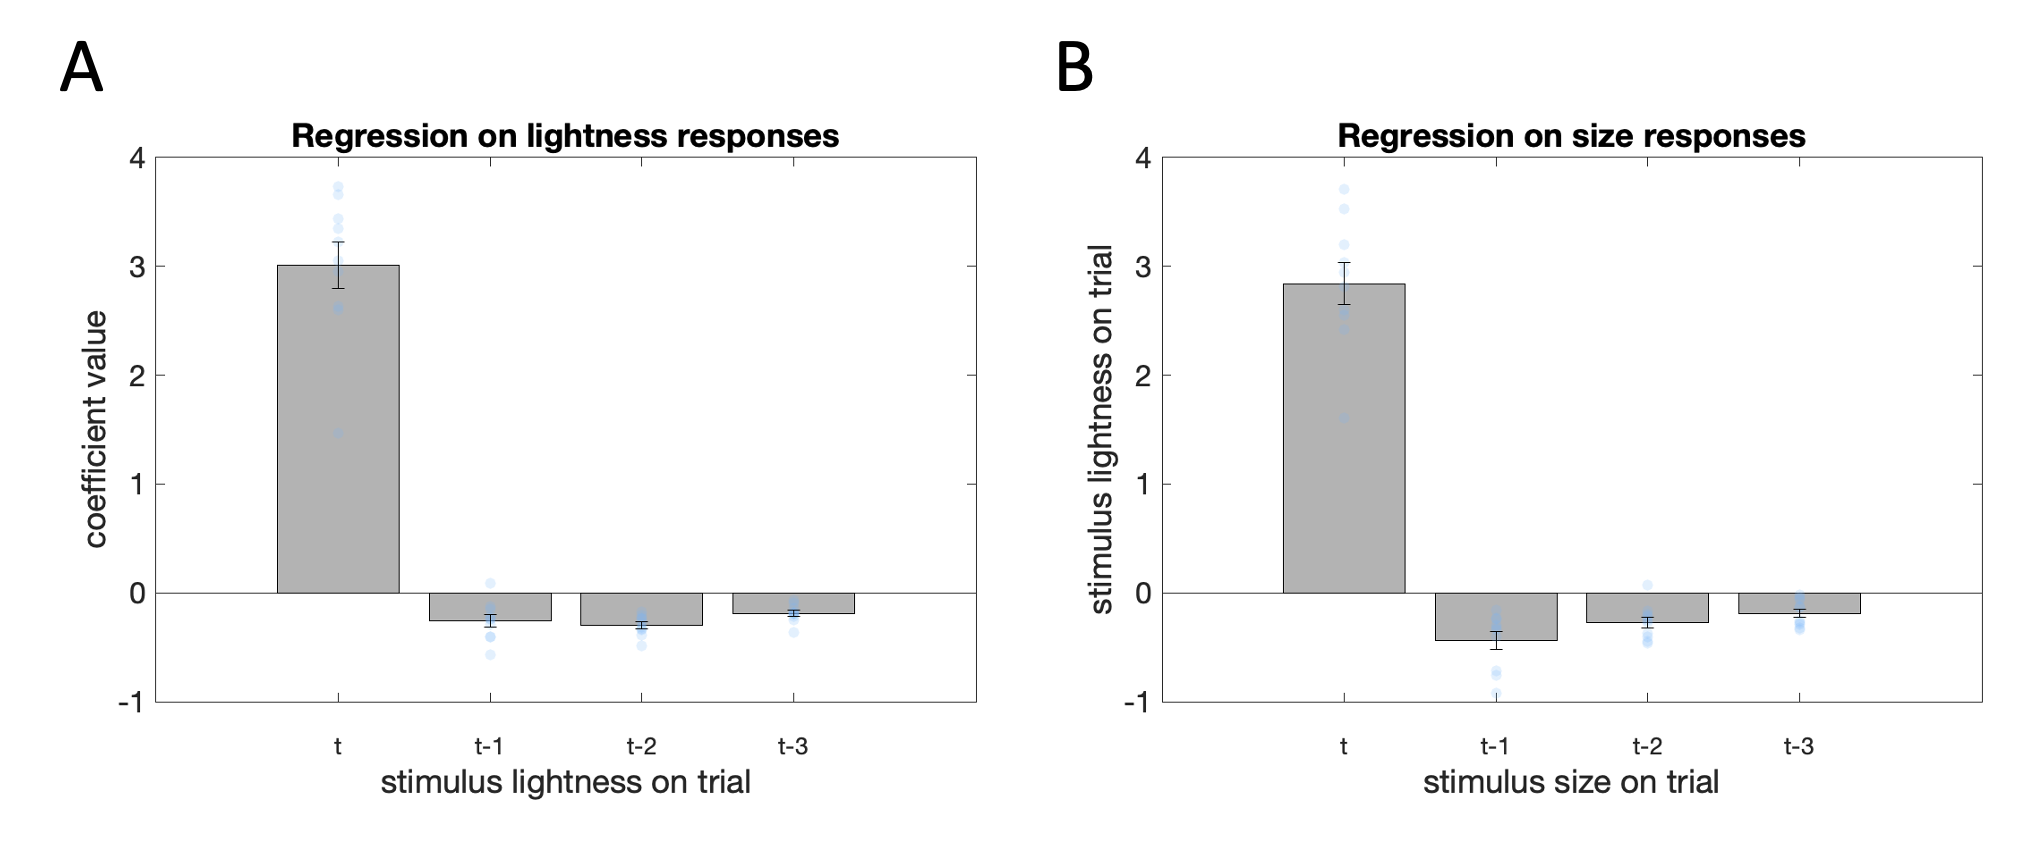
\includegraphics[width=1\linewidth]{figures/cat-reg-a} 

}

\caption[Experiment 1, Regression of responses on stimulus history]{Regression on stimulus history. Across both panels, the height of the bar depicts the average standardized coefficient value for the stimulus property value on the current trial (first bar: trial t), the stimulus property value on the immediately preceding trial (second bar: trial t-1), the stimulus property value on trial before last (second bar: trial t-2), and the stimulus property value three trials ago (second bar: trial t-3). Error bars depict SEM, blue dots show coefficient values for individual participants. $\textbf{A:}$ Coefficients for lightness responses. $\textbf{B:}$ Coefficients for size responses.}\label{fig:cat-reg-a}
\end{figure}

\hypertarget{interim-discussion-4}{%
\subsection{Interim Discussion}\label{interim-discussion-4}}

Temporal context yielded a significant influence on categorizations in Experiment 1. Category boundaries for size and lightness were higher when the temporal context was dominated by larger and lighter stimuli; categorization judgments were also repulsed from the task-relevant characteristics of the stimuli on preceding trials. The smaller the size of the preceding stimuli, the more likely the current stimulus to be categorized as large. Our experimental design allowed us to rule out response bias as a driver of the observed effects. In fact, temporal context biases decisions even when this would lead to a distortion in the relative frequency of actions. This is because in our design, the relative frequency of ground truth ``high'' and ``low'' judgments was carefully counterbalanced. Thus, context-dependent categorization necessarily skews the distribution of ``high'' vs ``low'' responses.

We did not find evidence that the contextual effect increases when each stimulus is presented for 1000ms versus 200ms. We predicted that longer stimulus durations would allow for additional adaptation to the stimulus set. Contrary to our prediction, for size, we found that \emph{shorter} stimulus durations led to stronger contextual biases. This finding may speak to the literature on the effect of noise on context-dependencies; shorter stimulus durations made the task more demanding. A Bayesian perspective dictates that this should lead to heavier reliance on the prior and consequently, stronger contextual biases. Interpreted in this light, our results appear to provide support for a Bayesian contraction bias mechanism driving the observed context dependence.

However, we did also find evidence that the contextual effect is not isolated to task-relevant information. Contrary to the predictions of a Bayesian process, which incorporated the distribution of recently experienced stimulus properties in a prior, we found that participants were also biased by task-irrelevant visual information. Categorization thresholds were higher in the brief condition where the task-irrelevant visual environment was lighter and larger. This suggests that a more automatic, sensory visual adaptation process, acting on our perception of the current to-be-categorized stimulus, likely contributes to the observed contextual dependencies. In Experiment 2, we follow up on these findings and assess more directly the contributions of adaptation.

\hypertarget{experiment-2-1}{%
\section{Experiment 2}\label{experiment-2-1}}

In Experiment 2, we aimed to disentangle the two putative sources of contextual influence -- changes to our representation of the category boundary (Fig. \ref{fig:cat-expl}a) versus changes to our experience of the current stimulus (Fig. \ref{fig:cat-expl}b). We took advantage of the fact that adaptation processes, which impact our perception of incoming input, are characterized by changes in sensitivity to the dominating characteristics in the environment. Thus, we estimated the contribution of adaptation to context-dependent categorization judgments by comparing participants' sensitivity to stimulus characteristics across two temporal contexts. We did this separately for the two visual properties from Experiment 1, size and lightness, as well as for a more abstract stimulus property -- numerosity. Computing numerical magnitudes engages later stages of processing compared to low-level visual properties, such as lightness, contrast or orientation \autocite{heng2020} and has been linked with various higher-level cognitive processes, which rely on an `approximate number system' \autocite{piazza2007,nieder2009}. Imprecision in the estimation of numerical magnitudes has also been put forth as the driver of biases in value-based decisions about economic prospects \autocite{woodford2020}. Consequently, including numerosity in this experiment allows us to link the current chapter more closely with context dependencies in economic decisions.

\hypertarget{methods-7}{%
\subsection{Methods}\label{methods-7}}

While Experiment 1 was conducted in the Perception Laboratory at the Department of Experimental Psychology, the pandemic prevented onsite data collection for Experiment 2. Thus, all data for this experiment were collected remotely.

\hypertarget{participants-5}{%
\subsubsection{Participants}\label{participants-5}}

Twenty participants (aged 28.3 ±8.63) with normal or corrected-to-normal vision took part in Experiment 2. The study received ethical approval from the Central University Research Ethics Committee at the University of Oxford (approval reference number: R55652/RE005). All participants provided written informed consent and were compensated with £10 per hour for their time.

\hypertarget{aparatus}{%
\subsubsection{Aparatus}\label{aparatus}}

Participants completed the experiment on their personal computers. The study was programmed using PsychoPy \autocite{peirce2007} and PsychoJS and was hosted on Pavlovia. The output (combined RGB) light intensities of all monitors were calibrated with a perceptual calibration method \autocite[half tone pattern matching,][]{xiao2011} or with a photometer (ColorCal, Cambridge Research Systems). Participants were instructed to set their monitors to the lowest brightness setting and to disable any automatic brightness adjustment or light filtering applications on their computers. We chose to conduct the perceptual calibration procedure at low brightness for two reasons. First, increasing the brightness settings on a monitor, might introduce a brightness offset (i.e.~requested 0\% lightness does not correspond to black pixel output, but produces some light), which would render the gamma model (\(y=x^{\gamma}\)) of the electro-optical transfer function of the monitor inaccurate. Second, human visual sensitivity to changes in brightness decreases with absolute brightness levels, and so, we can minimize variability in brightness matches by conducting them at a low brightness setting. This in turn ensures that our perceptual estimate of the electro-optical transfer function of the monitor, which is based on the brightness matches, is reliable.

Viewing distance was determined individually for each participant. We asked participants to adjust the size of a rectangle on their screen to match the size of a standard bank card \autocite{yung2015}. We used the size of the rectangle in pixels to calculate the required visual distance such that 1 pixel would subtend \(57''\) of visual angle; this ensured that the size of the stimuli in visual angle would be approximately the same for all participants.

\hypertarget{stimuli-4}{%
\subsubsection{Stimuli}\label{stimuli-4}}

The experiment consisted of three parts, each of which followed the same structure, but concerned a different stimulus property -- size, lightness or numerosity. In the size part of the study, the stimuli comprised grayscale circles presented against a black background. In the lightness part of the study, the stimuli comprised grayscale circles presented against a yellow background (as in Experiment 1). In the numerosity part of the study, the stimuli comprised clouds of black and white dots of varying sizes against a grey (half contrast) background. The color (white or black) was randomly selected for each dot, ensuring that the brightness of the stimulus would not be informative for the numerosity judgment. Following previous work, we also constrained the average dot radius or the total area covered by the dots to be the same across dot clouds in each trial \autocite{izard2008,vandenberg2017,heng2020}. For each trial, we randomly chose whether to hold dot radius or total area constant. This manipulation ensured that stimulus size neither on the level of individual dots nor on the level of the entire dot cloud would be informative for the numerosity judgment.

As in Experiment 1, for each of the three properties, we constructed an array of possible property values. The full arrays consisted of 10 possible values; the lowest 7 of those constituted the low stimulus set, and the highest 7 -- the high stimulus set. For size, the values ranged from 69 to 195 pixels in steps of 4 (corresponding to approximately \(1.1\)° to \(3.1\)° of visual angle). For lightness, the pixel values ranged between 0.35 and 0.65 in steps of 0.033 (assuming 0-1 range on an 8-bit monitor with linearized output intensities). For numerosity, the number of dots ranged from 8 to 52 in logarithmic steps, using a multiplier of 1.232.

\begin{figure}

{\centering 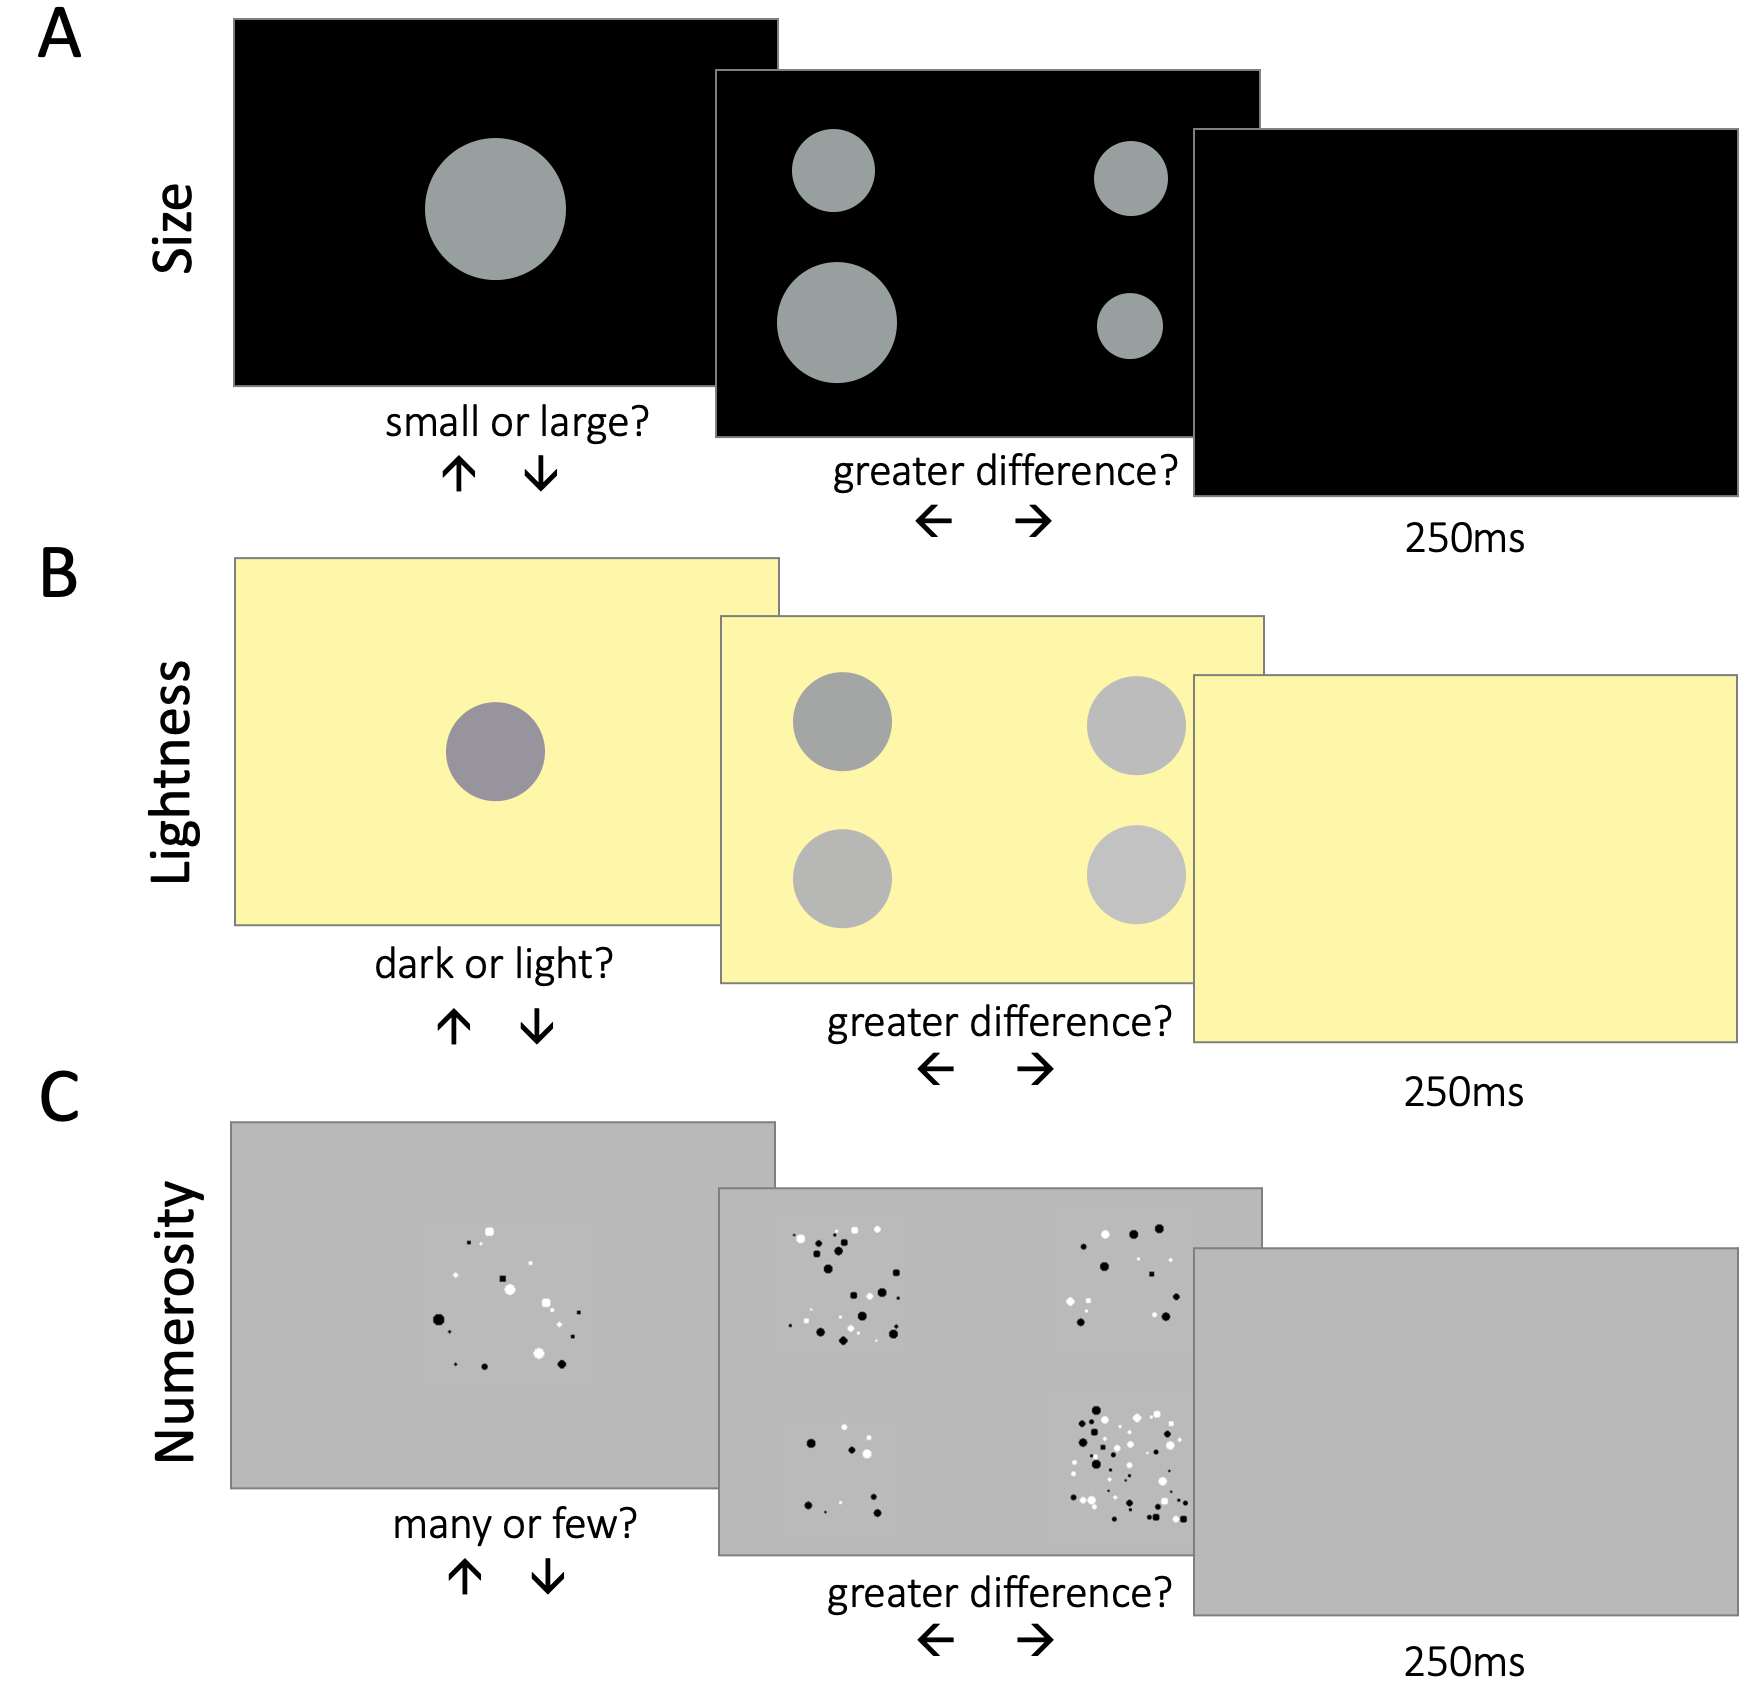
\includegraphics[width=1\linewidth]{figures/cat-trial-b} 

}

\caption[Experiment 2, Trial structure]{Trial structure. Across all parts of the experiment, categorization and difference comparison trials were interleaved. On categorization trials, participants saw a single stimulus in the center of the screen. On difference comparison trials, participants saw two pairs of stimuli, two stimuli on the left and two on the right size of the screen. $\textbf{A:}$ Part 1, size task. In categorization trials, participants had to categorize circle stimuli as large or small. They responded by pressing the up or down arrow key. In difference comparison trials, participants had to compare the difference in size between the two pairs of stimuli. If they considered the difference between the stimuli on the left larger than the difference between the stimuli on the right, they responded by pressing the left arrow key (and vice versa for right). $\textbf{B:}$ Part 2, lightness task. Participants had to categorize circle stimuli as light or dark, and compare the difference in lightness between the two pairs of stimuli. $\textbf{C:}$ Part 3, numerosity task. Participants had to categorize clouds of dots as many or few, and compare the difference in number between the two pairs of clouds.}\label{fig:cat-trial-b}
\end{figure}

\hypertarget{experimental-procedure-4}{%
\subsubsection{Experimental Procedure}\label{experimental-procedure-4}}

The experiment took approximately 3 hours, which participants were invited to complete over three shorter sessions. Links to the online experiments are available in the OSF repository (\url{https://osf.io/vxh3n/}) for this study. We did not counterbalance the order of the parts across participants, as the subjective difficulty of the tasks in the three parts increased progressively from size through lightness to numerosity.

Across all parts of the experiment, participants had to complete two types of tasks: categorization and difference comparisons. Participants' difference comparisons allowed us to estimate suprathreshold sensitivity. In categorization trials, participants saw a single stimulus in the center of the screen. In the size part, their task was to categorize the circle as large or small; in the lightness part -- to categorize the circle as light or dark; and in the numerosity part -- to categorize the number of dots in the cloud as many or few. Participants registered their choice via button press (up or down arrow). In difference comparison trials, participants saw two pairs of stimuli on the left and right side of the screen. Participants had to compare the two stimuli on the left, and decide whether the difference between them was larger than the difference between the two stimuli on the right. Thus, participants had to indicate which pair of stimuli was most different from one another. Again, they registered their choice via button press (left or right arrow). The stimuli remained on the screen for the full duration of the trial. The trial ended only when the participant provided a response.

Each part of the experiment comprised 4 blocks. Each block began with a series of 10 categorization trials, followed by 210 comparison and 210 categorization trials, presented in an interleaved fashion. We implemented the contextual manipulation during the categorization trials. In half of the blocks, the stimulus in categorization trials was drawn from the high stimulus set, and in the other half -- from the low stimulus set. This resulted in two contextual bias conditions -- low and high. Across all blocks, the stimuli in the difference comparison trials were drawn from the full stimulus set (i.e.~the 10 value array).

\hypertarget{analyses-5}{%
\subsubsection{Analyses}\label{analyses-5}}

First, we analyzed categorization trials. We estimated psychometric functions for the categorization decisions of each participant for each condition (low and high context) and each stimulus type (size, lightness and numerosity). As a sanity check, we confirmed that the contextual manipulation impacted categorizations, by comparing the threshold values for the low and high context conditions via paired samples \(t\) test.

Next, we analyzed difference comparison trials. We estimated sensitivity in the two conditions via maximum likelihood difference scaling \autocites[MLDS,][]{maloney2003,knoblauch2008}. MLDS constitutes a stochastic model of suprathreshold perceptual differences. The model assigns each of the 10 stimuli in the experiment a value on a latent perceptual scale, \(\psi_1\) to \(\psi_{10}\), such that the absolute differences between scale values (corresponding to the stimuli on a given trial) maximize the likelihood of the participant's response (the reported difference comparison). Since any linear transformation of the perceptual scale produces the same pattern of results, the model constrains the scale to span values between 0 and 1, (i.e.~\(\psi_1=0\) and \(\psi_{10}=1\)). Thus, there are 8 free \(\psi\) parameters (\(\psi_2\) to \(\psi_9\)) plus one additional free scaling term, \(\sigma\), which tracks the variability of participant responses. To assess whether the temporal context manipulation led to changes in suprathreshold sensitivity, we compared the perceptual scales estimated based on responses in the low condition (\(\psi_2^l\) to \(\psi_9^l\)) and responses in the high condition (\(\psi_2^h\) to \(\psi_9^h\)). More specifically, an adaptive process should lead to higher sensitivity for low stimulus magnitudes in the low context condition and higher sensitivity for high stimulus magnitudes a in the high context condition. We tested this prediction on the group level with a GLM, which quantified the impact of the contextual manipulation on participants' scale values (\(\psi_{2-9}^l\) and \(\psi_{2-9}^h\)), controlling for the nonindependence of scale values from the same observer and for the effect of stimulus level (2-9). To ascertain whether the effect of context was localized to a portion of stimulus space (e.g.~the lower of higher end of stimulus values), we also assessed the statistical significance and direction of the coefficient for the interaction between context and stimulus level via a GLM.

\hypertarget{computational-modeling-2}{%
\subsubsection{Computational Modeling}\label{computational-modeling-2}}

Finally, to bridge the results from categorical and difference comparison trials, we built one common model encompassing both tasks. At the heart of the model is the assumption depicted in Fig. \ref{fig:cat-expl}. That is, the model assumes that categorization decisions are based on the participant's representation of the stimulus (Fig. \ref{fig:cat-expl}b) and the participant's representation of the category boundary (Fig. \ref{fig:cat-expl}a), both of which might differ between contexts:
\begin{equation}
\begin{aligned}
r_{cat}^l = \frac{1}{1+\exp(-((x-c^l)-b^l) \cdot s^{-1})}\\
\\
r_{cat}^h = \frac{1}{1+\exp(-((x-c^h)-b^h) \cdot s^{-1})}
\end{aligned}
\end{equation}
where \(r_{cat}\) refers to the categorization decision, which is a logistic function of the stimulus property \(x\); the superscripts \(h\) and \(l\) denote the relevant context (high and low). The model comprises 2 free parameters tracking changes to the stimulus representation (\(c^l\) and \(c^h\)), and 2 free parameters tracking changes to the category boundary (\(b^l\) and \(b^h\)). The former two parameters determine the location of the transducer function along stimulus space, the latter two free parameters determine the location of the category boundary along stimulus space. A further free parameter, \(s\), determines the slope of the transducer which may differ between participants.

If the model were fit to categorization decisions only, the parameters tracking the contextual shift in the transducer would trade off with the parameters tracking the contextual shift in category boundary, and so, it would not be possible to reliably estimate both. However, difference comparison trials are based on the participant's representation of the stimulus \emph{only}, and not on the representation of the category boundary:
\begin{equation}
\begin{aligned}
y_i^l = \frac{1}{1+\exp-((x_i-c^l) \cdot s^{-1})} \\
\\
y_i^h = \frac{1}{1+\exp-((x_i-c^h) \cdot s^{-1})} \\
\\
r_{diff}^l = |y_1^l - y_2^l| - |y_3^l - y_4^l| \\
\\
r_{diff}^h = |y_1^h - y_2^h| - |y_3^h - y_4^h|
\end{aligned}
\end{equation}
where \(r_{diff}\) refers to the difference comparison decision, \(y_i\) refers to the representation of stimulus \(x_i\) and the subscript \(i\) tracks each of the four stimuli on a difference comparison trial. Thus, feeding information about participants' difference comparisons into the model allowed us to disentangle contextual changes to the representation of the stimulus (\(c^l\) versus \(c^h\)) from contextual changes to the representation of the category boundary (\(b^l\) and \(b^h\)).

We fit the model to empirical data from the experiment individually for each participant and each condition via gradient descent, implemented using the \texttt{globalsearch} algorithm from the MATLAB Optimization Toolbox. The best fitting parameter values allowed us to estimate the relative contributions of the two putative sources of influence to the contextual bias in categorizations. We did this by, first, calculating the contextual difference in the representation of the category boundary (\(\Delta(b)=b^h-b^l\)) and the contextual difference in the representation of the stimulus (\(\Delta(c)=c^h-c^h\)), as well as their sum (\(\Delta(total)=\Delta(b)+\Delta(c)\)); we then estimated their relative strengths (\(\frac{\Delta(c)}{\Delta(total)}\)).

\hypertarget{data-code-availability-statement-5}{%
\subsubsection{Data \& Code Availability Statement}\label{data-code-availability-statement-5}}

All data and code to reproduce the analyses are available in the OSF repository (\url{https://osf.io/vxh3n/}) for this project.

\hypertarget{results-7}{%
\subsection{Results}\label{results-7}}

Psychometric functions for categorization decisions are available in Fig. \ref{fig:cat-results-b}a; there is clear separation between low and high context conditions. Paired samples \(t\) tests on participants' threshold values for the two contexts confirm that categorization boundaries were higher in the high context across size (\(t_{18}=10.18\), \(p<0.0001\)), lightness (\(t_{18}=7.41\), \(p<0.0001\)), and numerosity (\(t_{18}=5.95\), \(p<0.0001\)) judgments (Fig. \ref{fig:cat-results-b}b). We excluded one participant from the main analyses, as visual inspection of their psychometric function indicated that they responded randomly on the categorization task for numerosity. We confirmed this by estimating the impact of the numerosity of each stimulus on that participant's categorization judgment via logistic regression (coefficient in the low condition \(b=0.04\), \(p=0.49\), coefficient in the high condition: \(b=0.05\), \(p=0.32\)).

\begin{figure}

{\centering 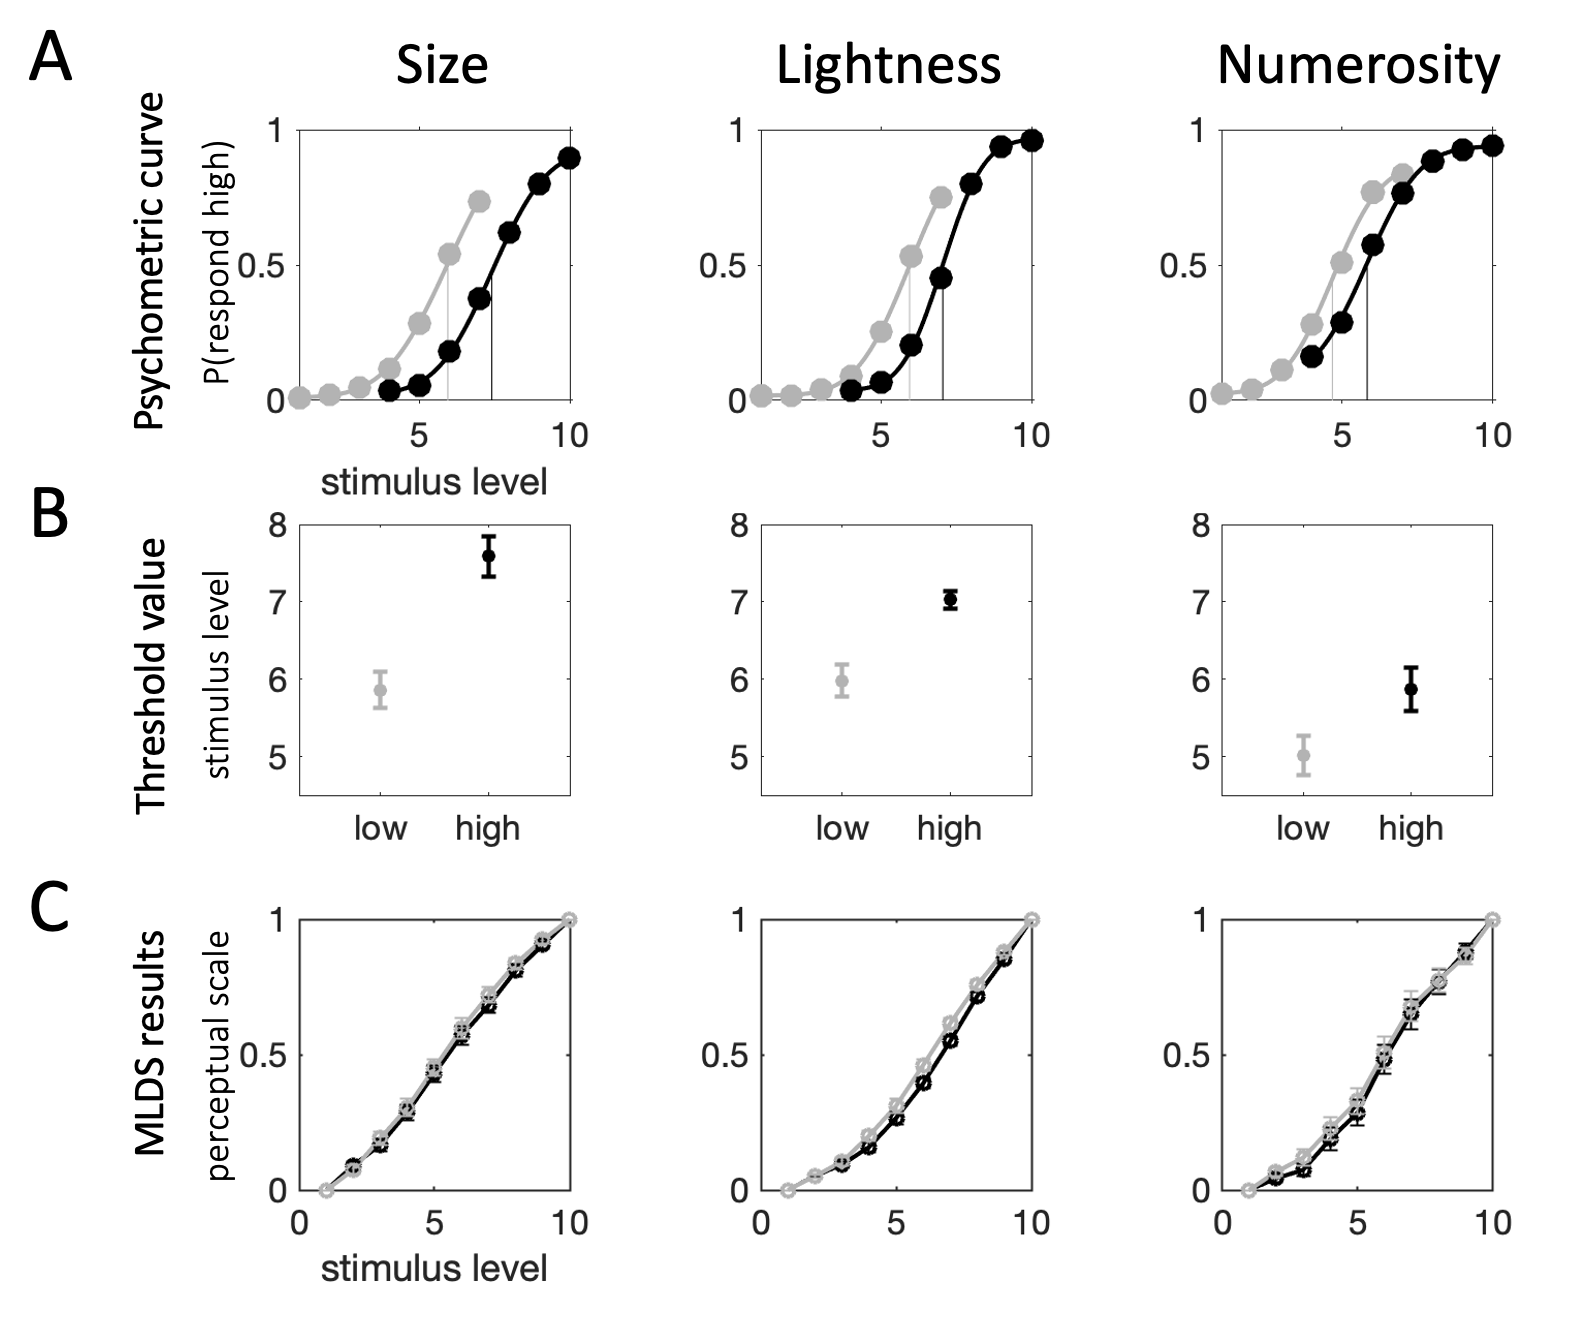
\includegraphics[width=1\linewidth]{figures/cat-results-b} 

}

\caption[Experiment 2, Psychometric functions and perceptual scales]{Experiment 2 results. Columns show results for each of the three different parts (left: size, middle: lightness and right: numerosity). $\textbf{A:}$ Psychometric functions based on aggregate data collapsed across participants. Points show raw data, curves -- cumulative Gaussian functions fit to data. Vertical lines show threshold value estimates for each condition. Shading indexes context condition (grey: low, black: high). Note that these average curves are for illustration purposes only, they are not necessarily representative of any one participant in the experiment. $\textbf{B:}$ Average threshold values (across all participants) for the two conditions (grey: low, black: high). Error bars depict SEM. $\textbf{C:}$ Perceptual scales for the two conditions (grey: low, black: high). Dots depict average scale value across participants, error bars depict SEM.}\label{fig:cat-results-b}
\end{figure}

Perceptual scales estimated from participants' difference comparison decisions are depicted in Fig. \ref{fig:cat-results-b}c.~The plots show the average estimates of perceptual scale values of all participants, error bars track SEM, shading denotes context. The distance between scale values (on the same perceptual scale) illustrates the estimated sensitivity -- the further away two points are, the more easily the participant can distinguish the stimuli they refer to. Thus, if the perceptual scale lay on the identity line (i.e.~all points were equidistant along the y-axis) then all stimuli would be equally discriminable, and so, participants would be equally sensitive to changes along stimulus space. Distortions to the perceptual scale, on the other hand, illustrate differential sensitivity. For instance, the more convex the perceptual scale, the higher the relative sensitivity for higher values of the stimulus property compared to lower values of the stimulus property. This means that the directionality of the dissociation between perceptual scales in the two contexts is important. An adaptive process should lead to higher sensitivity to high stimulus property values in the high context, and to low stimulus property values in the low context. Consequently, we would expect to see a more convex perceptual scale for the high context (i.e.~black curve below the grey curve).

The trends depicted by the average perceptual scales (Fig. \ref{fig:cat-results-b}c) seem to, on the whole, conform to this pattern. However, the effect appears small. Statistical tests confirmed that the contextual effect on sensitivity was reliable on the group level across all three stimulus types (size: \(\beta=0.10\), \(p<0.0001\), lightness: \(\beta=0.08\), \(p<0.0001\), numerosity: \(\beta=0.10\), \(p<0.0001\)). We did not find evidence that this effect was localized to the lower or higher end of stimulus space; the interaction between context and stimulus level was not statistically significant (size: \(\beta=-0.004\), \(p=0.20\), lightness: \(\beta=-0.005\), \(p=0.09\), numerosity: \(\beta=0.006\), \(p=0.22\)).

Finally, we estimated the relative contributions of the two putative sources of influence on context-dependent categorizations using our common model for the two types of tasks. Fig. \ref{fig:cat-model} shows the results of the model fitting exercise. The three values plotted on each panel depict the average estimates for the difference in parameter values for the internal representation of the stimulus (diamond dot: \(\Delta(c) = c^h - c^l\)), the difference in parameter values for the internal representation of the category boundary (square dot: \(\Delta(b) = b^h - b^l\)), and their sum (hexagonal dot: \(\Delta(total) = \Delta(c) + \Delta(b)\)), which tracks the contextual difference in categorization behavior between the two contexts.

Generally, model estimates are consistent with the results reported above. As can be seen from the plots in Fig. \ref{fig:cat-model}, for size and numerosity, the total contextual difference in categorization judgments (\(\Delta(total)\)) was driven primarily by changes to the representation of the category boundary (\(\Delta(b)\)). On average, differences in the representation of the category boundary explained 89\% and 73\% of the difference in categorization judgments for size and numerosity stimuli, respectively. For lightness, changes in the representation of the category boundary (\(\Delta(b)\)) contributed approximately 54\% of the difference in categorization judgments, suggesting that adaptation accounts for about half of the contextual bias in lightness categorizations.

\begin{figure}

{\centering 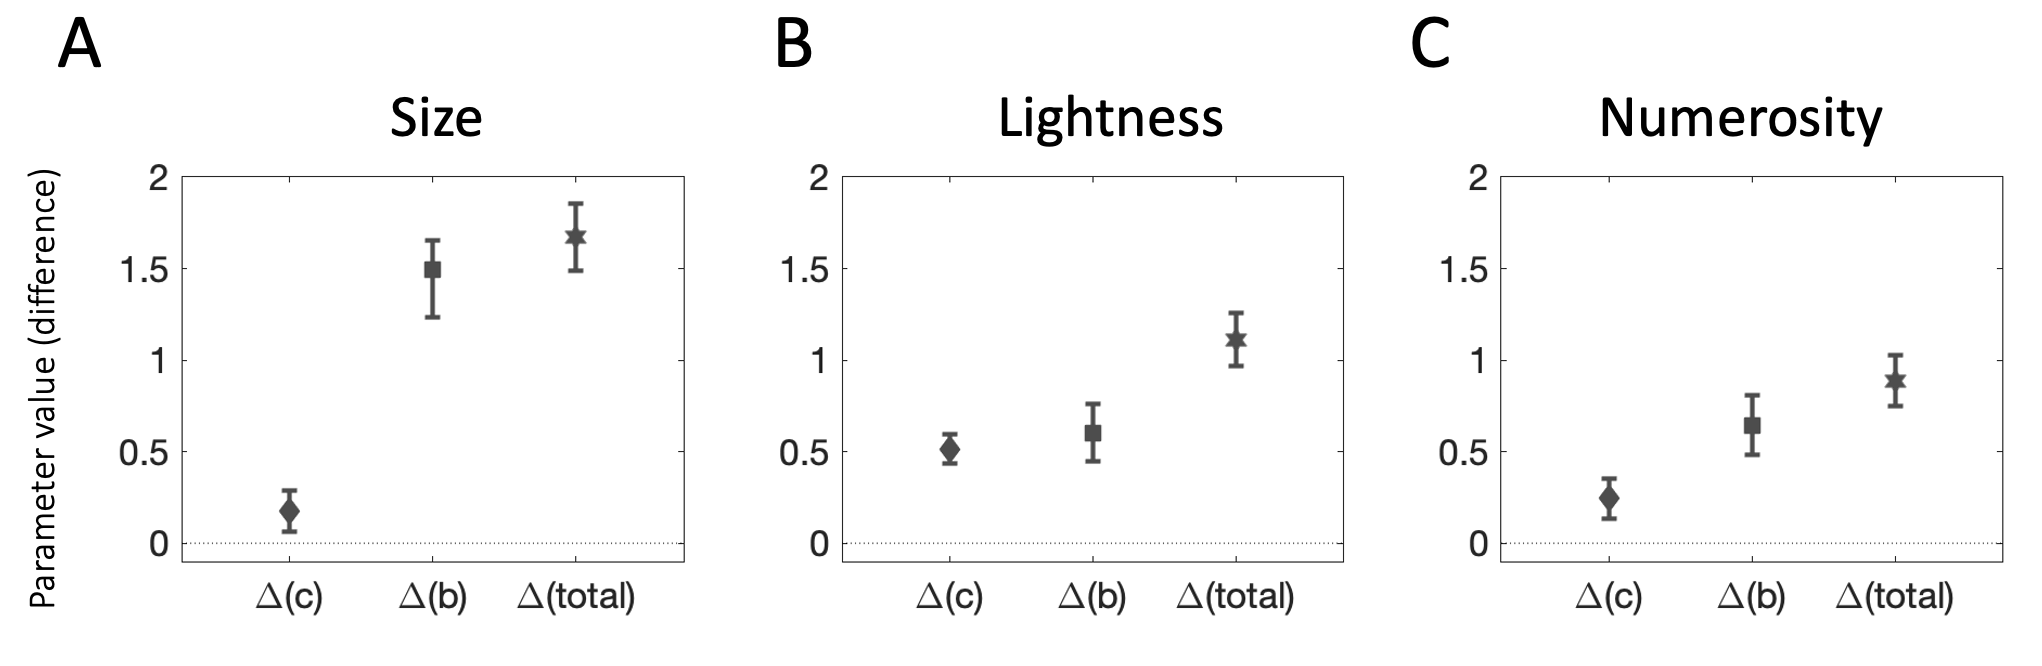
\includegraphics[width=1\linewidth]{figures/cat-model} 

}

\caption[Experiment 2, Model results]{Model results. Each panel depicts the difference in parameters between the high and low context conditions. The diamond-shaped dot corresponds to the difference between the parameters for the representation of the stimulus ($\Delta(c)$). The square dot corresponds to the difference between the parameters for the representation of the category boundary ($\Delta(b)$). The hexagonal dot corresponds to the total difference between parameters in the two conditions ($\Delta(total)$). Error bars track SEM. $\textbf{A:}$ Size task. $\textbf{B:}$ Lightness task. $\textbf{C:}$ Numerosity task.}\label{fig:cat-model}
\end{figure}

\hypertarget{interim-discussion-5}{%
\subsection{Interim Discussion}\label{interim-discussion-5}}

Experiment 2 also provided evidence for the robust influence of temporal context on categorization judgments. The effects held across all three properties we tested. When the context was dominated by larger, lighter and more numerous stimuli, category boundaries were pushed towards higher levels of size, lightness and numerosity. We found evidence that adaptation contributes to the observed context dependencies. On average, participants exhibited changes in sensitivity; however, those changes were modest in magnitude and differed between stimulus types. For lightness judgments, approximately half of the contextual bias can be captured by adaptation. For size and numerosity judgments, adaptation may account for 11\% and 28\% of the contextual bias. This pattern of results is consistent with the extensive literature on visual adaptation to light levels \autocite{reuter2011,barlow1972}, and the sparser literature on adaptation to size \autocite{blakemore1969,zimmermann2016} and higher level ``cognitive adaptation'' processes \autocite{palumbo2017a}. These results suggest that an adaptive encoding process adjusting the perception of a to-be-categorized stimulus contributes to the observed context dependencies in categorization.

\hypertarget{discussion-2}{%
\section{Discussion}\label{discussion-2}}

The temporal context in which a stimulus is situated affects how we choose to categorize it. Across two experiments, we replicate the robust contextual biases in categorization documented in the literature. When the temporal context is dominated by larger, lighter and more numerous stimuli, participants are more likely to categorize an objectively neutral stimulus as small, dark and low in number. We probed the computational origins of this bias.

The results of Experiment 1 demonstrated that context-dependent categorizations cannot be explained by a response bias driving an equal distribution of actions across contexts. Both experiments provide evidence that adaptation contributes to context dependencies in categorization decisions. Experiment 1 shows that contextual judgments are influenced by the visual environment beyond immediately task relevant inputs, consistent with the predictions of visual adaptation. Experiment 2 provides evidence that sensitivity to changes in stimulus characteristics shifts in a direction predicted by a normalization-based adaptive encoding process. The magnitude of the observed adaptation varies -- it is strongest for lightness, accounting for about half of the contextual bias in categorization decisions, and more modest in magnitude but significant for size and numerosity.

This adaptation process, however, does not lead to stronger contextual biases when each stimulus is experienced for 1000ms versus 200ms. This result speaks to the rich literature on the time courses of adaptation. Visual adaptation, for instance, has been documented to occur on timescales ranging between milliseconds to years over the course of an individual's lifetime \autocite{webster2015}. The dynamics of adaptation in the mammalian visual system vary with the past history of stimulation; the discriminability of changes to the stimulus characteristics as well as their statistical properties can also change the observed timescale of adaptation \autocite[measured over the course of seconds and minutes,][]{wark2009}. It is likely that all of these factors contribute to the adaptation effects we observe here. In Experiment 1, we manipulate context on the level of an experimental block (lasting \textasciitilde5 minutes), yet each stimulus is presented on the screen for a much briefer duration (\(\leq\) a second). Crucially, stimulus duration also varied on the block level, allowing the visual system to adjust to the timings of incoming stimuli and update the timescale of adaptation.

We found that shorter stimulus presentation led to \emph{more} context-dependent performance for size judgments. This finding is in line with a Bayesian hypothesis \autocite{olkkonen2014}, where reducing the duration of the stimulus increases task demands -- the participant has to remember the to-be-categorized stimulus as well as the category boundary in order to respond. This would lead participants to rely more heavily on the prior and so the contextual bias would be stronger, as in our size results. In Experiment 2, we estimated that contextual changes to the category boundary, akin to a Bayesian drift towards the stimulus characteristics dominating the temporal context, account for approximately the half of the context dependence observed in lightness judgments and the majority of the contextual influence in size and numerosity decisions.

Somewhat counter-intuitively, this Bayesian process produces an anti-Bayesian pattern of behavior. Typically, we might expect Bayesian influences on behavior to lead to judgments which are positively associated with the features present in the temporal context. In fact, this is exactly what happens in the commonly documented phenomenon of serial dependence, whereby choices concerning a typically noisy stimulus are attracted towards (or positively influenced by) the properties of the preceding stimulus \autocite{fischer2014,kiyonaga2017}. This effect makes sense in our temporally autocorrelated sensory (and conceptual) environment. Input on time \(t\) is typically strongly correlated with input on time \(t-1\). For instance, visual scenes tend to be relatively stable over time, so if there is uncertainty about the identity of an input, previous stimulation would serve as a useful cue as to its identity. In the laboratory, however, trials are randomized and carefully counterbalanced, and so, any such adaptation effect would lead to suboptimal choice behavior biased towards an objectively unrelated and irrelevant stimulus on the preceding trial.

Here, we see the opposite pattern. In our experiments, categorization decisions are repulsed away from the properties of the stimuli on preceding trials (Fig. \ref{fig:cat-reg-a}) as well as from the properties dominating the temporal context more generally (Fig. \ref{fig:cat-psychom-a}). This discrepancy in results is driven by a difference in task demands. In tasks where participants exhibit serial dependence, there is typically some uncertainty concerning the imperative stimulus -- e.g.~it has been presented prior to a short delay and so participants need to rely on a memory of the sensory experience, rather than on the sensory experience directly \autocite{hollingworth1910,kiyonaga2017}. To resolve that uncertainty, the neural system uses information from the temporal context like, for instance, the identity of the immediately preceding stimulus or some prior distribution of stimulus properties shaped by recent experience. The task we consider here is different. Participants need to categorize (or label) a stimulus that is currently available to them. Thus, there is no uncertainty about the imperative stimulus, the uncertainty lies in the category boundary -- i.e.~what should be the criterion for categorization? Thus, the prior distribution is incorporated in the standard \emph{against} which participants judge the stimulus, and so, the observed effects on behavior are repulsive.

The reach of these context dependencies extends far beyond the laboratory. This is because we base our actions on how we evaluate or categorize a given stimulus or situation. If our judgments are affected by information in the temporal context, then so too will our actions exhibit robust context dependencies. According to behavioral ecology, context dependence in judgments relating to sustenance maximizes an organism's chance for survival \autocite{stephens1986,kolling2012}. When deciding whether to stick to the current resource or forage for something better, it only makes sense to expend valuable energy on foraging if it is likely that better resources would be available in the environment. Thus, our definition of an acceptable banana should change depending on context. If the available bananas are predominantly unripe, we might happily eat a banana that is a bit on the green side. Conversely, a spotted, overripe banana might make the cut in a context dominated by rotting, brown bananas.

Context, however, impacts our judgments far beyond these evolutionarily relevant realms where context dependence may serve an adaptive, fitness-maximizing purpose. For instance, an ethics review committee should maintain stable standards for the ethicality of research proposals. Yet, we know that when student volunteers are faced with this task, their decisions to accept or reject a research proposal are significantly impacted by the levels of ethicality currently dominating the context \autocite{levari2018}. In the realm of political science, the context dependence of human judgment is encapsulated in the Overton window, a term coined in the 1990s by political commentator Joseph Overton. It refers to the range of ideas that are acceptable to the public, and it can shift and expand with the evolution of public opinion. Recently, analyses have highlighted how manipulating what information dominates the public sphere can be used to alter what the general public considers acceptable \autocite{greenhill2018,bobric2021}. Research into the mechanisms underlying the context dependence of human judgments, such as our study described here, bears implications for this line of work. Cognitive neuroscience can help inform the social sciences about when and how context affects behavior and what can be done to counteract it.

\hypertarget{conclusion-2}{%
\section{Conclusion}\label{conclusion-2}}

Context consistently sways categorization decisions across perception, cognition and economics. This chapter examined the computational mechanisms underlying this effect. We found that context dependencies in categorization behavior cannot be explained by a response bias, aiming to maintain the distribution of actions stable across contexts. Instead, our results suggest that context dependencies are driven by a combination of two complementary processes. The first process affects our representation of the category boundary, pushing it towards the central tendency of the context (Bayesian contraction bias). The second process affects our perception of the to-be-categorized stimulus, repelling it away from the properties of temporal context (adaptation). These two processes appear to contribute equally to the context dependence of lightness categorizations; however, the role of adaptation is weaker, yet significant, for judgments of stimulus size and numerosity.

\hypertarget{discussion-3}{%
\chapter{Discussion}\label{discussion-3}}

\minitoc

The optimality of our actions is constrained by the accuracy of our judgments. Yet, our percepts and evaluations often appear inaccurate. Depending on the context, the exact same alternatives might lead to different choices -- seemingly irrelevant contextual information biases our judgments in a consistent and systematic manner. This robust context dependence, thus, poses a puzzle. Why has evolution sculpted the neural system to process information in a manner that reduces the apparent accuracy of our judgments? I argued for the adaptive role of such a mechanism. Adjusting neural responses based on contextual information boosts the efficient encoding and processing of information; contextual information also helps resolve ambiguities in the face of noise and uncertainty.

In this discussion, I will summarize the findings from my doctoral work and highlight their implications for and connections with phenomena outside the scope of perception and economics, and outside the laboratory. My thesis considered three different instances of context-dependent choice across the realms of perception and economics. Each study combined careful experimental investigation of human behavior with simulations using mathematical models of hypothesized computational mechanisms. This approach allowed me to first, chart the parametric influence of context on human choices, and second, arbitrate between different theoretical accounts of the drivers of the observed context dependencies. On the behavioral level, the studies revealed rich patterns of contextual influence spanning interactive, attractive and repulsive effects. On the algorithmic level, my computational work provided evidence that normalization schemes of neural processing can account for many of the observed contextual effects.

\hypertarget{overview-of-results}{%
\section{Overview of Results}\label{overview-of-results}}

Chapter 2 introduced decoy effects in economic multialternative choice. It went beyond existing work in the field, which has traditionally focused on three well established decoy effects (attraction, compromise and similarity), and mapped the strength and directionality of decoy influence across the full two-dimensional attribute space. Computational simulations revealed that the rich structure of decoy influence can be produced by a simple, general principle of relative encoding, where attribute values are repulsed away from the context of rival options. In the chapter, I further explored the space of putative normalization schemes and charted their predicted behavioral signatures in the multialternative choice task. Evidence from the choice behavior of a large cohort of human volunteers converged with normalization theories that compressively transduce inputs, appealing to normalization by the central tendency of context and recurrently overweighing the contribution of the target input to the normalization.

Chapter 3 considered the role of this information processing scheme in the domain of perceptual choices along a single visual dimension -- orientation. Evidence from three psychophysical experiments indicates that perceptual distractors exert an interactive influence on choices, biasing the accuracy of judgments according to their consistency with target input. This result is in stark contrast with the classic model of distractor influence, which proposes that distractors compete with targets for processing resources and attract choices as a function of the observer's attention. Instead, I find that focusing attention enhances sensitivity to target stimuli, but does not ameliorate the contextual influence of the distractor. This counter-intuitive finding is consistent with an attention-independent normalization coding scheme, where the gain with which target signals are processed is boosted in consistent contexts, a mechanism which presumably lies outside of voluntary control.

Finally, chapter 4 delved into the computational mechanisms of context-dependent categorization decisions. Through rigorous experimental design, I provide evidence that the observed contextual bias is driven by the combined influence of a normalization-based information processing scheme, continuously adapting to the temporal context of the decision maker, and a Bayesian process, pushing the categorization standards towards the central tendency of context. This finding holds across three distinct stimulus dimensions -- lightness, size and numerosity -- highlighting the domain-generality of the mechanisms underlying the observed context dependence, and bridging our results with related work on context dependence in evaluations of propositional statements and subjective value.

\hypertarget{interpretation}{%
\section{Interpretation}\label{interpretation}}

Taken together, the results of the three studies in this thesis contribute a unifying account of context dependencies across perceptual and economic decisions. Across all chapters, normalization emerged as a common theme, offering a compelling computational account of the behavioral results. It is perhaps somewhat counter-intuitive that a common neural mechanism would drive context dependencies across all the scenarios I consider here. They do, after all, concern very different stimulus characteristics, spanning visual appearance and subjective value, and pose distinct task demands, including comparing, categorizing and ordering alternatives. Yet, divisive normalization has been identified as a ``canonical neural computation'', repeated across brain regions and modalities \autocite{carandini2012}. It might, thus, form part of an arsenal of operations that the neural system has evolved to apply across the processing hierarchy for a variety of problems.

The existence of a common computational mechanism underlying relative judgment has long been hypothesized in the psychological literature. Adaptation-level theory \autocite[ALT,][]{helson1964}, for instance, posits that the human brain processes all manner of information in a relative manner. According to ALT, inputs are evaluated against the current adaptation level of the individual, which is shaped by the stimulation present in the temporal and spatial context (residual and background stimuli, respectively, in ALT). ALT strove to provide a unified account of context dependencies across perception, affect, motivation, learning, cognition and interpersonal behavior. Research on contextual effects across these areas has since, however, splintered off into distinct and largely theoretically unrelated research streams, like for instance, work on adaptation and perceptual constancy in perception \autocite{smithson2005,webster2015} and work on the hedonic treadmill in well-being research \autocite{diener2009a}. The parallels between the underpinnings of context dependencies in perceptual and economic choices highlighted in this thesis signal that there is merit in considering the relativity of human judgment holistically and renewing the search for a domain-general computational mechanism of contextual influence.

\hypertarget{zooming-out}{%
\section{Zooming Out}\label{zooming-out}}

\hypertarget{context-dependence-in-the-wild}{%
\subsection{Context Dependence in the Wild}\label{context-dependence-in-the-wild}}

The instances of context dependence I considered here differ in their definitions of context. Chapters 2 and 3 considered the influence of information present in the spatial context of a decision. In chapter 3, this information was completely irrelevant to the choice problem; the contextual input constituted a distractor stimulus which the decision maker was asked to ignore. In chapter 2, this information formed part of the choice set; the decision maker was asked to evaluate the contextual (decoy) input and assign a preference rank to it. Chapter 4, on the other hand, considered temporal context. The contextual input consisted of stimuli on previous trials. The task demands in the laboratory rendered context ``irrelevant'' for the evaluation of the imperative stimulus across all three of these definitions. Yet, outside the artificial laboratory setting, where stimuli and trials are independently and randomly sampled, the irrelevance of context is not so clear cut.

Context may provide useful cues for the interpretation of information. The Kuleshov effect, for instance, refers to a phenomenon whereby the same (ambiguous) facial expression can be interpreted as showing different and potentially contradictory emotions depending on the context in which it is encountered. Popularized by filmmaker Lev Kuleshov over a century ago, the effect emerged when the same clip of an actor was stitched together with oppositely valenced scenes, a scene of a funeral or a scene of a child playing. In the former case, the actor's emotional state was interpreted as melancholy, in the latter -- as happiness \autocite{mobbs2006}. It is easy to see why using context as a cue in this situation would be compelling. In daily life, the emotions of the people around us do usually covary with the context in which they are situated. It is primarily in artificial settings, like the psychology laboratory, that facial expressions may be divorced from their surroundings and need to be interpreted following \emph{unrelated} emotionally charged clips \autocite{mobbs2006} or photographs \autocite{mullennix2019}.

Context is, thus, useful to make sense of the world. In fact, its role in helping us interpret inputs is so crucial that it features prominently in attempts to construct artificial brains. Context dependencies are inbuilt in various state-of-the-art artificial neural networks. Convolutional networks (CNNs) incorporate information from the spatial context of inputs to analyze and classify images. The base operations of CNNs largely mirror the structure of the visual system, with convolutional and pooling layers serving an analogous computational role as simple and complex cells \autocite{lindsay2021}. Similarly, recurrent networks (RNNs) incorporate information from the temporal context of inputs to interpret information sequences. Analogous processes, where signals are dynamically fed back to processing units, are commonly found in biological brains \autocite{goulas2021}. Context dependence is, hence, ubiquitous and crucial across both biological and artificial information processing operations.

\hypertarget{context-dependence-as-a-tool}{%
\subsection{Context Dependence as a Tool}\label{context-dependence-as-a-tool}}

Reliance on context is a compelling strategy in the real world, but it can also lead to inconsistent and inaccurate behavioral outcomes. The same processes that I describe in this thesis -- decoy \autocite{wu2020} and repulsive ``contrast'' effects \autocite{levin2002} -- are often applied by marketing professionals to influence consumer choices. Artificially constructing choice contexts that can tip consumer preferences towards a desired alternative is a lucrative avenue for private companies; recent estimates show that decoy effects can increase sales by as much as 15\% \autocite{wu2020}. There is, thus, a clear financial incentive to understand and take advantage of contextual influences on decisions.

Beyond purchasing choices, unintended contextual biases can arise in various social settings, like for instance, the selection of candidates in hiring and admissions decisions \autocite{highhouse1996,norton2004,simonsohn2013}. Raising the stakes does not seem to eliminate the influence of context. Context dependencies sway even the (arguably) most consequential decisions in society concerning policy choices \autocite{herne1997} and political leadership \autocite{chang2019}. Archival electoral data and experimental surveys demonstrate that voting choices in American electoral races systematically violate the normative principle of independence of irrelevant alternatives \autocite{sueocurry1995,chang2019}.

Over the past decade, a movement to harness these robust context dependencies ``for good'' has garnered momentum \autocite{thaler2008}. The central idea of the movement is that policy makers can ``nudge'' individuals towards better decisions about, for instance, their retirement savings and health care, by designing choice contexts which bias people towards the desired outcomes. This approach is often called libertarian paternalism: manipulating the decision context (e.g.~how choice alternatives are ordered or presented) would not affect decision makers' freedom to choose. It would, however, ensure that if the decision makers were to behave in a context-dependent manner, they would choose the intended option determined by a presumably benevolent entity.

Translating research on choice context dependencies into nudges has been the focus of governmental nudge units, such as the the UK's Behavioural Insights Team and (previously) the USA's Social and Behavioral Sciences Team. Economically, nudging approaches are estimated to be several times more cost-effective than traditional public policy interventions, such as tax incentives and other financial inducements \autocite{benartzi2017}. In the domain of retirement savings, for instance, nudging has been implemented to boost enrollment rates, prompt individuals to choose more appropriate retirement plans and increase their savings contributions \autocite{benartzi2007,iyengar2010}. More recently, there has been an increased interest in applying contextual choice biases to prompt individual action in response to the climate crisis \autocite{schubert2017,zaneva2020,carlsson2021}.

The success of green nudges and other similar choice interventions, however, is constrained by our understanding of context dependence in human choice. Despite their ever growing popularity, little is actually known about why and how nudging interventions work \autocite{marteau2020}. Rigorous methodological evaluations, which are largely missing from the field \autocite{marchiori2017,vankleef2018}, and controlled experiments, like the ones presented in this thesis, are necessary to develop a theoretical understanding of the observed behaviors and mechanisms underlying them. Building that understanding is key for the optimization of choice architecture interventions and the maximization of their impact.

\hypertarget{conclusion-3}{%
\section{Conclusion}\label{conclusion-3}}

Why do people do what they do? The behavioral sciences aim to address this big question. The study of decision making is crucial for this endeavor, since our actions are, generally, guided by our decisions. It is particularly important to understand the decision process in those cases when our actions appear inconsistent or inaccurate. Oftentimes, inconsistencies can be traced back to reliance on irrelevant contextual information. Uncovering why context matters for our decisions is important not only as a theoretical venture (e.g.~what are the neural mechanisms?, are humans rational?, etc.), but also has important translational implications. Context dependence can be wielded as a tool to protect our best interests, as is the goal of the nudge movement. It may, however, also be applied against those interests. It is, thus, crucial to understand and be aware of manipulations to the choice context.

This thesis contributes to a body of work that aims to further our collective understanding of precisely those processes. My doctoral work compiled evidence on context-dependent choice across the domains of perception and economics. Through careful experimental manipulations, I mapped the behavioral signatures of contextual effects. I combined this data with computer simulations to shed light on the information processing mechanisms underlying context-dependent choice. Taken together, these tools can help uncover the factors and processes driving context dependencies in decision making, bringing us one small step closer to answering the big question.


%%%%% REFERENCES
\setlength{\baselineskip}{0pt} % JEM: Single-space References


{\renewcommand*\MakeUppercase[1]{#1}%
\printbibliography[heading=bibintoc,title={\bibtitle}]}


\end{document}
